\documentclass[a4paper,10pt]{article}

\usepackage{color}
\usepackage{xcolor}
\usepackage{tikz}
\usepackage{amsmath}
\usepackage{amssymb}
\usepackage{amsthm}
\usepackage{graphicx}
\usepackage{mathtools}
\usepackage{wrapfig}
\usepackage{multirow}
\usepackage{comment}
\usepackage{natbib}
%\usepackage{float}
\usepackage{appendix}
\usepackage{enumitem}
\usepackage{newfloat}
\usepackage{subcaption}
\usepackage[utf8]{inputenc}
\usepackage{floatrow}
\usepackage{bm}
\usepackage{hyperref}
\usepackage{tcolorbox}
\usepackage{chngcntr}

\usetikzlibrary{calc}
\usetikzlibrary{fit}
\usetikzlibrary{decorations.shapes,shapes.misc,calc, positioning, hobby, backgrounds}


%\DeclarePairedDelimiter{\floor}{\lfloor}{\rightfloor}
%\DeclarePairedDelimiter{\ceil}{\lceil}{\rceil}

\newcommand{\denominator}{\ensuremath{n+\sum\limits_{j=1}^{h} k_{j}}}
\newcommand{\halflength}{\ensuremath{\floor{\frac{m}{2}}}}
\newcommand{\floor}[1]{\left \lfloor #1 \right \rfloor}
\newcommand{\ceil}[1]{\left \lceil #1 \right \rceil}
\newcommand{\pospart}[1]{\left( #1 \right)_{+}}
\newcommand{\negpart}[1]{\left( #1 \right)_{-}}
\newcommand{\set}[2]{\left\{ #1 \, | \, #2 \right\}}

\tikzset{cross/.style={cross out, draw=black, minimum size=2*(#1-\pgflinewidth), inner sep=0pt, outer sep=0pt},
%default radius will be 1pt. 
cross/.default={1pt}}

\tikzset{decorate sep/.style 2 args=
{decorate,decoration={shape backgrounds,shape=circle,shape size=#1,shape sep=#2}}}


\newtheorem{theorem}{Theorem}[section]
\newtheorem{corollary}[theorem]{Corollary}
\newtheorem{lemma}[theorem]{Lemma}

\theoremstyle{definition}
\newtheorem{definition}[theorem]{Definition}

\theoremstyle{definition}
\newtheorem{example}[theorem]{Example}
 
\theoremstyle{remark}
\newtheorem*{remark}{Remark}

\theoremstyle{definition}
\newtheorem*{note}{Note}

\DeclareFloatingEnvironment[fileext=los,
    listname={List of Example Figures},
    name=Example Figure,
    placement=tbhp,
    within=section,]{examplefigure}
    
\DeclareFloatingEnvironment[fileext=los,
    listname={List of myFigures},
    name=Figure,
    placement=tbhp,
    within=section,]{myfigure}    
    
\counterwithin{figure}{section}

\title{Patrolling games on graphs collection}
\date{\today}
\author{Thomas Lowbridge \\ School of Mathematical Sciences \\ University of Nottingham}

\bibliographystyle{plain}

\begin{document}

\pagestyle{empty}
{
  \renewcommand{\thispagestyle}[1]{}
  \maketitle
  This document houses all work on patrolling games on graphs.
  \tableofcontents  
}
\clearpage
\pagestyle{plain}


\setlength{\parindent}{0pt}
\setlength{\parskip}{1em}

\newpage
\pagenumbering{arabic}

%This section will introduce the game and basic properties
\section{Introduction to game}
\subsection{Pure game}
A patrolling game $G=G(Q,T,m)$ is a win-lose, zero-sum game between a maximizing patroller (often referred to as she) and a minimizing attacker (often referred to as he). The parameters of the game are:
\begin{itemize}
\item The graph $Q$ which has a set of nodes, $N$,  and of edges, $E$.
\item The length of time over which the game takes place, the time-horizon $T$.
\item The length of time the attack takes to complete, the attack-time $m$.
\end{itemize}

Two forms of the game exist: the one-off game, which is played in a finite time interval $\mathcal{T}=\{0,1,...,T-1\}$ denoted using $G^{o}$; and the periodic game, which is played on the time circle $\mathcal{T}^*=\{0,1,...,T-1\}$ (with the asterisk representing arithmetic on the time circle taking place modulo $T$) denoted using $G^p$. We will assume that $T \geq m$ , otherwise all attacks will fail.

The pure strategies available to the patroller are called patrols, choosing a starting position and how to walk along the graph Q, $W:\mathcal{T} \rightarrow N$. With no restrictions in the one-off game, but the restriction that the edge $(W(T-1),W(0)) \in E$ in the periodic game (so that $W(T)=W(0)$). Let $$\mathcal{W}=\{ W \, | \, W:\mathcal{T} \rightarrow N \text{ s.t } (W(t),W(t+1)) \in E \text{ for } t=0,...,T-2  \} $$ be the set of all pure patrols in the one-off game (and similarly $\mathcal{W}^*$ in the periodic game). Let there be some ordering to the strategies $W_{k} \in \mathcal{W}$ (or $W_{k} \in \mathcal{W}^{*}$) for $k=1,...,|\mathcal{W}|$ (or $k=1,...,|\mathcal{W}^*|$ in the periodic game).

The pure strategies available to the attacker are pairs, $[i,I]$ for $i \in N$, called the attack node, and $I=\{ \tau,\tau+1,...,\tau+m-1 \} \subseteq \mathcal{T}$ (or $I \subseteq \mathcal{T}^*$ if periodic) called the attack interval (starting at time $\tau$). Let $\mathcal{A}=\{[i,I] \, | \, i \in N , I \subseteq \mathcal{T} \}$ be the set of all possible pure attacks. Let there be some ordering to the strategies $A_{k} \in \mathcal{A}$ for $k=1,...,|\mathcal{A}|$.

A patrol, $W$, intercepts the attack, $[i,I]$, if $i \in W(I)=\{W(\tau),W(\tau+1),...,W(\tau+m-1)\}$ and as our game is Win-Lose the pure payoff function is
$$P(W,[i,I])=\left\{ \begin{array}{l}
1 \text{  if  } i \in W(I) ,\\
0 \text{  if  } i \notin W(I) .\\
\end{array}\right.$$
A pure payoff matrix $\mathcal{P}=(P(W_{i},A_{j}))_{i \in \{ 1,...,|\mathcal{W}| \}, j \in \{ 1,...,|\mathcal{A}| \}}$ (with the change of $\mathcal{W}$ to $\mathcal{W}^*$ if in the periodic game) stores Win ($1$) or Lose ($0$) for each pair of pure strategies.

\subsection{Mixed game}
Let $\Pi_{W}$ be the set of mixed strategies for the patroller in the one-off game and $\Pi_{W}^*$ in the periodic game. Let $\Phi$ be the set of mixed strategies for the attacker.

In the mixed strategy game the patroller selects a strategy $\bm{\pi} \in \Pi_{W}$ (or $\bm{\pi}  \in \Pi_{W}^*$ in the periodic game).

The attacker selects a strategy $\bm{\phi} \in \Phi$. Then the mixed payoff function (Probability of Capture) is

$$
P(\bm{\pi} ,\bm{\phi})=\sum\limits_{i=1}^{|\mathcal{W}|} \sum\limits_{j=1}^{|\mathcal{I}|} \mathcal{P}_{i,j} \bm{\pi} _{i} \bm{\phi}_{j}
=\bm{\pi} \mathcal{P} \bm{\phi}
$$
(with the change of $\mathcal{W}$ to $\mathcal{W}^*$ if in the periodic game).
%We will use $P(\pi,\phi,i)$ for $\pi \in \Pi_{W}$ , $\phi \in \Phi$ and $i \in N$ to mean the probability of capture at the node $i$.

We will also use the convention that a pure strategy is in the mixed strategy set, $W_{i} \in \Pi_{W}$ (or $W_{i} \in \Pi_{W^*}$) and $A_{j} \in \Phi$, to mean $\bm{\pi}_{k}=\left\{\begin{array}{c}
1 \text{ if } k=i, \\
0 \text{ if } k \neq i. \\
\end{array} \right.$
and
$\bm{\phi}_{k}=\left\{\begin{array}{c}
1 \text{ if } k=j, \\
0 \text{ if } k \neq j. \\
\end{array} \right.$ respectively

The value of the game is denoted by $V=V(Q,T,m) \equiv \max\limits_{\bm{\pi} \in \Pi} \min\limits_{\bm{\phi} \in \Phi} P(\bm{\pi},\bm{\phi})=\min\limits_{\bm{\phi} \in \Phi} \max\limits_{\bm{\pi} \in \Pi} P(\bm{\pi},\bm{\phi})$ and when needed we distinguish between the one-off and period game by using the subscripts $V^{o}$ and $V^p$ respectively.

\subsection{Properties}


%This section will explain all the Current Tools used to solve such problems
\section{Current Reduction Tools}


\subsection{Symmetry}
Symmetry of a graph's nodes allows us to reduce the number of attacks and patrols under consideration. This is because symmetric nodes must be treated identically (or some bias is formed for the other player). More formally

\begin{definition}[Attacker Equivalence]
We call two nodes, $n_{1}$ and $n_{2}$, \textit{equivalent} if there exists some automorphism, $\sigma$, of $Q$ which takes one to the other, i.e $n_{1}=\sigma (n_{2})$ or $n_{2}=\sigma (n_{1})$. Two attack intervals, $I_{1}$ and $I_{2}$, are called \textit{equivalent}  if there exists some automorphism, $\gamma$ on the time interval, $\mathcal{T}$ which is reflective, i.e $\gamma(t)=T-t$.
\end{definition}

\begin{lemma}[Attacker Symmetry]
We only need to consider the equivalence class of nodes for the attacker, with the same attack pattern formed on the equivalent nodes. Similarly we need only consider the equivalence class of attack times. Furthermore the periodic game has all attack times equivalent (under some rotation of the time circle) so only the node need be considered.
\end{lemma}

\begin{definition}[Patroller Equivalence]
We call two patrols, $W_{1}(t)$ and $W_{2}(t)$, \textit{equivalent} if there exists some automorphism, $\sigma$, of $Q$ takes one two the other, i.e $W_{1}(t)=\sigma (W_{2}(t))$ or $W_{2}(t)=\sigma (W_{1}(t))$.
\end{definition}

\begin{lemma}[Patroller Symmetry]
We only need to consider the equivalence class of patrols for the patroller, with the same patrol pattern formed on the equivalent patrols.
\end{lemma}

So without affecting the value of the graph we can reduce the problem to one of searching through the equivalent class of strategies for both players.

\subsection{Strategy Domination}
Domination of some strategies for the patroller and attacker are given, which allows the removal of these strategies from the possible strategy space for the players.

\begin{note}
We use the term dominance to mean weak dominance.
\end{note}

\begin{lemma}[Waiting Patrol Dominated]
For $Q$ connected and $T \geq 3$, $m \geq 2$ , patrols staying at any node for three consecutive periods are dominated.
\end{lemma}

\begin{corollary}[Penultimate Attack Dominated]
For $m \geq 3$, attacks at penultimate (i.e non-leaf node adjacent to a leaf node) nodes are dominated.
\end{corollary}

\begin{myfigure}
\begin{center}
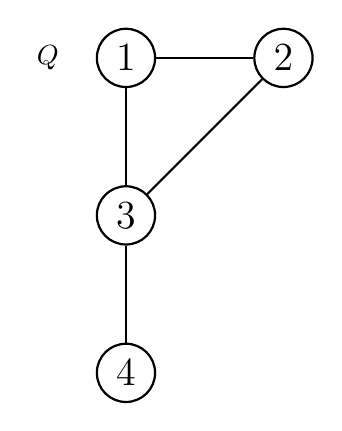
\begin{tikzpicture}[baseline=(current bounding box.north),-,auto,node distance=2cm,
                    thick,main node/.style={circle,draw,font=\sffamily\Large\bfseries}]

  \node[main node] (1) {$1$};
  \node[main node] (2) [right of=1] {$2$};
  \node[main node] (3) [below of=1] {$3$};
  \node[main node] (4) [below of=3] {$4$};

  \path[every node/.style={font=\sffamily}]
    (1) edge  (2)
    edge (3)
    (2) edge (3)
    (3) edge (4);
    
\node [left=0.5cm,text width=0.5cm] at (1)
{
$Q$
};  
\end{tikzpicture}
\end{center}
\caption{Graph Q used for examples}
\label{fig: Q}
\end{myfigure}

\begin{example}
For $Q$ as seen Figure \ref{fig: Q} We can see that nodes, $1$ and $2$, are equivalent nodes by using the automorphism $\sigma(1)=2$, $\sigma(2)=1$, $\sigma(i)=i \quad \forall i \neq 1,2$. Similarly the patrols ${W_{1}(t)=\left\{\begin{array}{l}
1 \text{ for } t \text{ even} \\
3 \text{ for } t \text{ odd} \\  
\end{array}\right.} \quad \text{and} \quad {W_{2}(t)=\left\{\begin{array}{l}
2 \text{ for } t \text{ even} \\
3 \text{ for } t \text{ odd} \\  
\end{array}\right.}$ are equivalent under the same automorphism.

The patrol ${W_{3}(t)=\left\{\begin{array}{l}
1 \text{ for } t=1,2,3  \\
3 \text{ for } t \geq 4 \\  
\end{array}\right.}$ is dominated (by $W_{1}(t)$)

Node $3$ is penultimate and so will not be attacked.
\end{example}


\section{Bounds}
\subsection{Basic Bounds(Attacker and Patroller)}
We seek bounds on the value of the game $V$. The lower bounds are given in terms of the patroller's ``good'' strategy against all attacker options, similarly the upper bounds are given in terms of the attacker's ``good'' strategy against all the patroller options. When we reach tightness between the bound these ``good'' strategies become an optimal solution.

By the patroller waiting a random node they can achieve $V \geq \frac{1}{n}$ and by the attacker picking a random node with a fixed time $I$ they can achieve $V \leq \frac{m}{n}$ (More generally $V \leq \frac{\omega}{n}$ for $\omega$, the maximum number of nodes any patrol can cover).

\begin{lemma}[General bounds]
$$\frac{1}{n} \leq V \leq \frac{\omega}{n} \leq \frac{m}{n}$$
Where $\omega$ is the maximum number of distinct nodes that can be visited in an attack interval.
\end{lemma}

\subsection{Decomposition(Patroller)}
We can consider decomposing the graph so that we just operate on parts with some appropriate probability.

\begin{lemma}[Decomposition lower bound]
Consider decomposing $Q$ into edge-preserving subgraphs $Q_{i}$ for $i=1,...,k$ with values $V_{i}=V(Q_{i})$ such that $Q=\bigcup\limits_{i=1}^{k} Q_{i}$ then
$$V \geq \frac{1}{\sum\limits_{i=1}^{k} \frac{1}{V_{i}}} $$
Furthermore in the case of a disjoint decomposition equality is reached
\end{lemma}

More explicitly an edge-preserving subgraph is a subgraph who has all possible connection between its nodes and disjoint means both edge and vertex disjoint. This means we are really only selecting nodes for the subgraph and the edges are mandated.The above provides a solution to build disjointly decomposable graphs, so it is only worth studying connected graphs.


\begin{example}
For $Q$ as seen in Figure \ref{fig: Q}. Consider when $m=3$, the decomposition of $Q$ into the graphs $Q_{1}$ and $Q_{2}$ (as in Example Figure \ref{examplefig:Q Decompisition}). $V_{1}=V(Q_{1})=1$ as alternating between $1$ and $2$ can catch every attack. $V_{2}=V(L_{3})=\frac{3}{4}$ (as seen in \cite{Alpern2011} ). 

Then we can get the bound $V \geq \frac{1}{(\frac{1}{1}+\frac{3}{4})}=\frac{4}{7}$.
\end{example}

\begin{myfigure}
\begin{center}
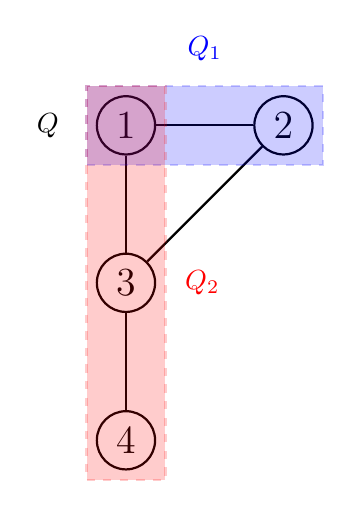
\begin{tikzpicture}[baseline=(current bounding box.north),-,auto,node distance=2cm,
                    thick,main node/.style={circle,draw,font=\sffamily\Large\bfseries}]

  \node[main node] (1) {$1$};
  \node[main node] (2) [right of=1] {$2$};
  \node[main node] (3) [below of=1] {$3$};
  \node[main node] (4) [below of=3] {$4$};

  \path[every node/.style={font=\sffamily}]
    (1) edge  (2)
    edge (3)
    (2) edge (3)
    (3) edge (4);
  
  \node (Box1) [draw=blue,dashed,thick,fit=(1) (2),fill=blue,opacity=0.2] {};  
  \node (Box2) [draw=red,dashed,thick,fit=(1) (3) (4),fill=red,opacity=0.2] {};
  
  \node [yshift=3.0ex, blue] at (Box1.north) {$Q_{1}$};
  \node [xshift=3.0ex, red] at (Box2.east) {$Q_{2}$};  
\node [left=0.5cm,text width=0.5cm] at (1)
{
$Q$
};   
\end{tikzpicture}
\end{center}
\caption{Decomposition of Q into \textcolor{blue}{$Q_{1}$} and \textcolor{red}{$Q_{2}$}.}
\label{examplefig:Q Decompisition}
\end{myfigure}

\subsection{Simplification(Patroller and Attacker)}

\begin{definition}[Node Identification]
The operation of Node identification on two nodes, $u$ and $v$, of a graph, $G=(N,E)$ into a single node $w$, is a mapping $f:N \rightarrow N'$ resulting in a new graph $G'=(N',E')$ where $N'=(N \setminus  \{u,v\}) \cup \{w\}$ with $E'=E \setminus \{(u,v)\}$ if $(u,v) \in E$ and under the condition that $\forall x \in N$, $f(x) \in N'$ is incident to $e' \in E'$ iff $e \in E$ is incident to $x \in N$.
Furthermore if a graph, $Q$, undergoes repeated node identification to become $Q'$ then we say it has been simplified. 
\end{definition}

\begin{definition}[Embedded walk]
An \textit{Embedded walk}, $W'$, on $Q'$ is the walk, $W$, done on $Q$ under the simplification mapping of $Q$ to $Q'$. i.e if $\pi :Q \rightarrow Q'$ is the simplification map, then $W'=\pi (W)$.
\end{definition}

\begin{lemma}[Simplification]
If $Q'$ is a simplified version of $Q$ then $V(Q') \geq V(Q)$
\end{lemma}

This allows us to get bounds for both the patroller and attacker.

\begin{example}
For $Q$ as seen in Figure \ref{fig: Q}. Consider when $m=3$, the Simplification of the graph by identifying $1,2$ from $Q$ to $Q'=L_{3}$ (as seen in Example Figure \ref{examplefig:Q Simplification}). Hence we can get the bound that $V(L_{3}) \geq  V(Q)$ hence $V(Q) \leq \frac{3}{4} $
\end{example}

\begin{myfigure}
\begin{center}
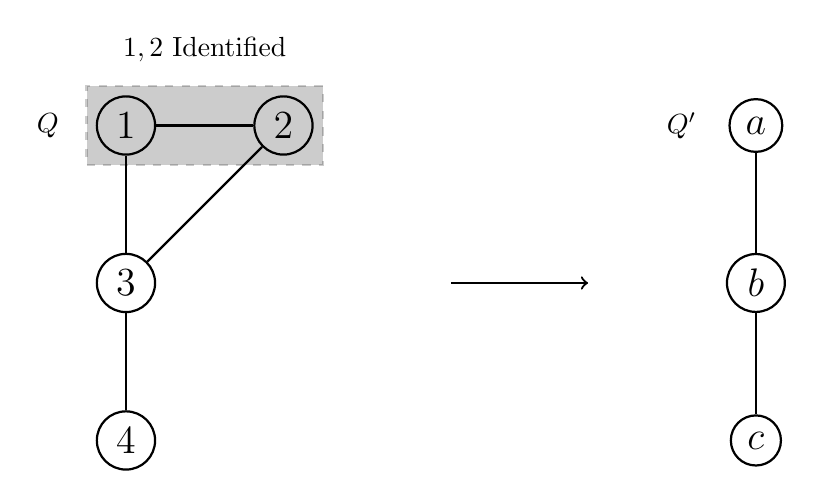
\begin{tikzpicture}[baseline=(current bounding box.north),-,auto,node distance=2cm,
                    thick,main node/.style={circle,draw,font=\sffamily\Large\bfseries}]

  \node[main node] (1) {$1$};
  \node[main node] (2) [right of=1] {$2$};
  \node[main node] (3) [below of=1] {$3$};
  \node[main node] (4) [below of=3] {$4$};
  
  \node (P1) [below of=2] {};
  \node (P2) [right of=P1] {};
  \node (P3) [right of=P2] {};
  
  \draw[->] (P2) edge (P3);
  
  \node[main node] (b) [right of=P3] {$b$};
  \node[main node] (a) [above of=b] {$a$};
  \node[main node] (c) [below of=b] {$c$};

  \path[every node/.style={font=\sffamily}]
    (1) edge  (2)
    edge (3)
    (2) edge (3)
    (3) edge (4)
    (a) edge (b)
    (b) edge (c);
  
  \node (Box1) [draw,dashed,thick,fit=(1) (2),fill,opacity=0.2] {};  
  
  \node [yshift=3.0ex] at (Box1.north) {$1,2$ Identified};  
\node [left=0.5cm,text width=0.5cm] at (1) {$Q$};
\node [left=0.5cm,text width=0.5cm] at (a) {$Q'$};   
\end{tikzpicture}
\end{center}
\caption{Simplifcation of $Q$ to $Q'$ by identification.}
\label{examplefig:Q Simplification}
\end{myfigure}


\subsection{Old Diametric attack(Attacker)}
Let $d(i,i')$ is the distance between nodes $i$ and $i'$ with the distance measured by the minimum number of edges.

\begin{definition}[Graph Diameter]
The diameter of a graph $Q$ is definded by $\bar{d}=\max\limits_{i,i' \in N} d(i,i')$ . The node pairs satisfying this are called diametrical.
\end{definition}

\begin{lemma}
By the attacker playing equally likely at a pair of diametrical at a random time interval, called the diametric attack, gives $V \leq \max\left\{\frac{m}{\raisebox{-0.5ex}{$\scriptstyle 2 \bar{d}$}} , \frac{1}{2} \right\}$
\end{lemma}

However the bound presented in \citep{Alpern2011} seems to indicate for large $T,m$ the second is chosen. However a simple counter example will show the bound does not allows hold
\begin{example}[Problem with diametric attack]
\label{example:counterexamplediamater} 
Consider the graph $L_{5}$ so $\bar{d}=4$ for $T=m=5$, then under the diametric attack, the patroller performing the patrol $\{ 1,2,3,4,5 \}$ allows her to catch the two attacks. Hence the bound of $V \leq \frac{5}{8}$ given by lemma does not seem to hold. 
\end{example}



\subsection{Covering(Patroller) and Independence(Attacker)}

\begin{definition}[Covering]
A patrol, $W$, is called \textit{intercepting} if it intercepts every possible attack at every node contained in the patrol, i.e all nodes visited by $W$ are in any subpath of length $m$ (i.e visits are at most $m$ apart).

A set of intercepting patrols forms a \textit{Covering set} if every node in $Q$ is contained in at least one of the patrols. Furthermore the \textit{Covering number}, $\mathcal{C}$ is the minimum cardinality of all the covering sets.
\end{definition}

\begin{definition}[Independence]
Two nodes, $i$ and $i'$, are called independent (under attack time, $m$) if any patrol intercepting an attack at $i$ cannot also intercept an attack at $i'$.

For the one-off game this is equivalent to $d(i,i') \geq m$.

For the Periodic game this is equivalent to $d(i,i') \geq m$ and $2d(i,i') \leq T$(due to returning to start).

A set of independent points forms a \textit{Independent set} if every element of the set is independent of every other element. Furthermore the independence number $\mathcal{I}$ is the maximum cardinality of all the independent sets.
\end{definition}

Clearly $\mathcal{I} \leq \mathcal{C}$ as to cover a collection of independent nodes, at least that many covering patrols are needed (Possibly more if they also don't get every node in $Q$)

\begin{lemma}[Covering and Independence]
$$ \frac{1}{\mathcal{C}} \leq V \leq \frac{1}{\mathcal{I}} $$
\end{lemma}


\section{Simple Graph bounds and solutions}

\subsection{Hamiltonian}
A Hamiltonian graph is a graph with a Hamiltonian cycle. Two simple examples of such graphs are cyclic graphs, $C_{n}$ and the complete graph, $K_{n}$. While Hamiltonian graphs can exhibit more than one Hamiltonian cycle we shall assume that we have selected one. We shall also assume that the attack, $m < n$, as otherwise by following the Hamiltonian cycle we guarantee capture (i.e for $m \geq n$, $V=1$).

\begin{definition}[Random Hamiltonian Patrol]
A \textit{Random Hamiltonian Patrol} is a mixed strategy starting with equal probability at all nodes and following the Hamiltonian cycle.
\end{definition}

\begin{theorem}[Hamiltonian]
If $Q$ is Hamiltonian, by following the Random Hamiltonian Patrol (if feasible), the patroller can achieve $V \geq \frac{m}{n}$.
\end{theorem}

This, along with a general upper bound from \citep{Alpern2011}, provides the solution $V=\frac{m}{n}$.

Two common Hamiltonian graphs are the Cyclic graph (of n nodes $C_{n}$) and the Complete graph (of n nodes $K_{n}$).
\begin{center}
\begin{figure}

\begin{tabular}{@{}c@{}}
  \begin{tabular}{c}
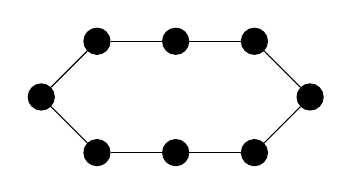
\begin{tikzpicture}[baseline=(current bounding box.north),-,auto,node distance=1cm,
                    main node/.style={circle,draw,fill=black,font=\sffamily\bfseries}]

  \node[main node] (1) {};
  \node[main node] (2) [above right of=1] {};
  \node[main node] (3) [right of=2] {};
  \node[main node] (4) [right of=3] {};
  \node[main node] (5) [below right of=4] {};
  \node[main node] (6) [below left of=5] {};
  \node[main node] (7) [left of=6] {};
  \node[main node] (8) [left of=7] {};
  

  \path[every node/.style={font=\sffamily}]
  (1) edge (2)
  (2) edge (3)
  (3) edge (4)
  (4) edge (5)
  (5) edge (6)
  (6) edge (7)
  (7) edge (8)
  (8) edge (1);

   
\end{tikzpicture}
     
      \\ \small $C_{8}$
  \end{tabular} \qquad
  \begin{tabular}{c}
  
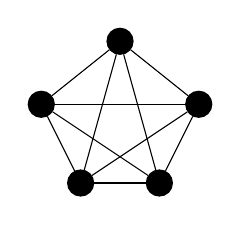
\begin{tikzpicture}[baseline=(current bounding box.north),-,auto,node distance=1cm,
                    main node/.style={circle,draw,fill=black,font=\sffamily\bfseries}]

  \node[main node] (1) {};
  \node[main node] (2) [shift={(1,-0.8)}] at (1) {};
  \node[main node] (3) [shift={(0.5,-1.8)}] at (1) {};
  \node[main node] (4) [shift={(-0.5,-1.8)}] at (1) {};
  \node[main node] (5) [shift={(-1,-0.8)}] at (1) {};

  

  \path[every node/.style={font=\sffamily}]
  (1) edge (2)
      edge (3)
      edge (4)
      edge (5)
  (2) edge (3)
      edge (4)
      edge (5)    
  (3) edge (4)
      edge (5)
  (4) edge (5);


   
\end{tikzpicture}

 \\ \small $K_{5}$
  \end{tabular} \\
\end{tabular}
\caption{Examples of Cyclic and Complete graphs}
\end{figure}
\end{center}

\subsection{Biparite}
A bipartite graph is a graph which can be partitioned into two sets, $A$ and $B$ (with $|A|=a,|B|=b$, assume WLOG that $b \geq a$) were edges only exist between these two sets. A special bipartite graph is the complete bipartite graph $K_{a,b}$.

Assume that $m < 2b$, as otherwise there exists a $2b$ period patrol which covers all nodes and guarantees capture (i.e if $m \geq 2b$, $V=1$).

\begin{definition}[Bipartite Attack]
The \textit{Bipartite Attack} selects nodes equiprobably from the larger set $B$ for a fixed time interval, $I$ (or for the two time intervals, $I$ and $I+1$ equiprobably).
\end{definition}

\begin{theorem}[Bipartite]
If $Q$ is bipartite with $b \geq a$, by following the Bipartite Attack, the attacker can achieve $V \leq \frac{m}{2b}$
\end{theorem}

The reasoning behind the bound is that any patrol must alternate between $|A|$ and $|B|$, so only visits a node from $B$ every other time step. 

\subsection{Complete Bipartite}
\begin{corollary}[Complete Bipartite]
The value of the complete bipartite graph, $K_{a,b}$, with $b \geq a$, then $V=\frac{m}{2b}$.
\end{corollary}

This is because a lower bound of $V \geq \frac{m}{2b}$ is given by the random Hamiltonian patrol in $K_{b,b}$ , which simplifies to $K_{a,b}$.

The star graph, $S_{n}$ is a graph with a centre and $n$ nodes adjacent to the centre.

\begin{corollary}[Star]
The value of $S_{n} \equiv K_{1,n}$ is $V=\frac{m}{2n}$.
\end{corollary}

\section{Line graph}






%
\section{New Bounds}

\subsection{Problem and Correction of diametric attack}
Consider the patroller strategy against a diametric attack that simply oscillates between the two diametric points.

The total number of attacks the attacker is making under this diametric strategy is $2(T-m+1)$, we will now measure how many the simple strategy for the patroller gets.

We will divide the set of captured attacks, depending on what is happening. This division shall be into start captures, middle captures and end captures.

The start captures are captures catching less than $m$ attacks in the early times, i.e before the middle. The middle captures are captures catching exactly $m$ attacks. The end captures are captures catching less than $m$ attacks in the late times.

\begin{example}[Problem with diametric attack]
Consider the graph $L_{5}$ so $\bar{d}=4$ for $T=20$,$m=6$, then under the diametric attack, the patroller oscillating between diametrics points gets.
\begin{itemize}
\item[Start] Capture $1+5=6$ attacks initially.
\item[Middle] Capture $6+6=12$ attacks when arriving at node $5$.
\item[End] Capture $4$ attacks when finishing at node $1$.
\end{itemize}
Giving $22$ out of $2(20-6+1)=30$ attacks, a better than $\frac{3}{4}$ value.
\end{example}

First off it is worth considering that the number of end attacks that are going to be caught will come from two values (if more than these would be in the middle). We could suggest that waiting at the start is more preferable to ``stabilize'' into the middle quicker. the cost for doing so is to remove one from each end value, if one of the end values is 1, then the penultimate middle is also reduced by 1 and thus becomes an end value.

While each time we decide to wait gains us 1 for each node in the start values, until it becomes a middle value. As $m \geq \bar{d}$, we are guaranteed that there are at least two start values (as we are looking at times $0$ and $\bar{d}-1 < m$). Therefore it is certain that waiting at the start (at least while there are two start values) is not worse than the just oscillating strategy.

Therefore we can wait until $t=m-(\bar{d}-1)$ (which as $m > \bar{d}-1$ means its is always possible), then this is only the start.

Let us count the pattern under this strategy,
\begin{itemize}
\item[Start:] Capture $m-\bar{d}$ attacks initially by waiting.
\item[Middle:] Capture $m \times (\floor{\frac{T-2m+1}{\bar{d}}}+1)$ attacks in the middle cycles (if any middle times are possible, otherwise zero if negative).
\item[End:] Capture $T-1-(m-1+(\floor{\frac{T-2m+1}{\bar{d}}}+1)\bar{d})$ (at the penultimate node visit (if possible, this really is zero if its negative) and $T-1-(m-1+(\floor{\frac{T-2m+1}{\bar{d}}}+2)\bar{d})$ at the final node visit (again zero if negative).
\end{itemize}

This gives \begin{align*}
& m-\bar{d}+\pospart{m \times (\floor{\frac{T-2m+1}{\bar{d}}}+1)} + \\ &\pospart{T-(m-1+(\floor{\frac{T-2m+1}{\bar{d}}}+1)\bar{d})} + \pospart{T-(m-1+(\floor{\frac{T-2m+1}{\bar{d}}}+2)\bar{d})}
\end{align*}

We will call $\alpha=\floor{\frac{T-2m+1}{\bar{d}}}$

\begin{lemma}[Condition on $T$ for bound to hold]
When $T=m-1+(k+1)\bar{d}$ for some $k \in \mathbb{N}_{0}$ then the diametric bound holds. Otherwise as $T \rightarrow \infty$ then the diametric bound holds.
\end{lemma}

Proof: \ref{Condition on T for old diametric proof}

\begin{figure}
%\includegraphics[scale=0.4]{DiametricAttack(m_45,d_30)1.png}
\resizebox{0.95\linewidth}{!}{
% Created by tikzDevice version 0.10.1 on 2017-11-09 12:03:49
% !TEX encoding = UTF-8 Unicode
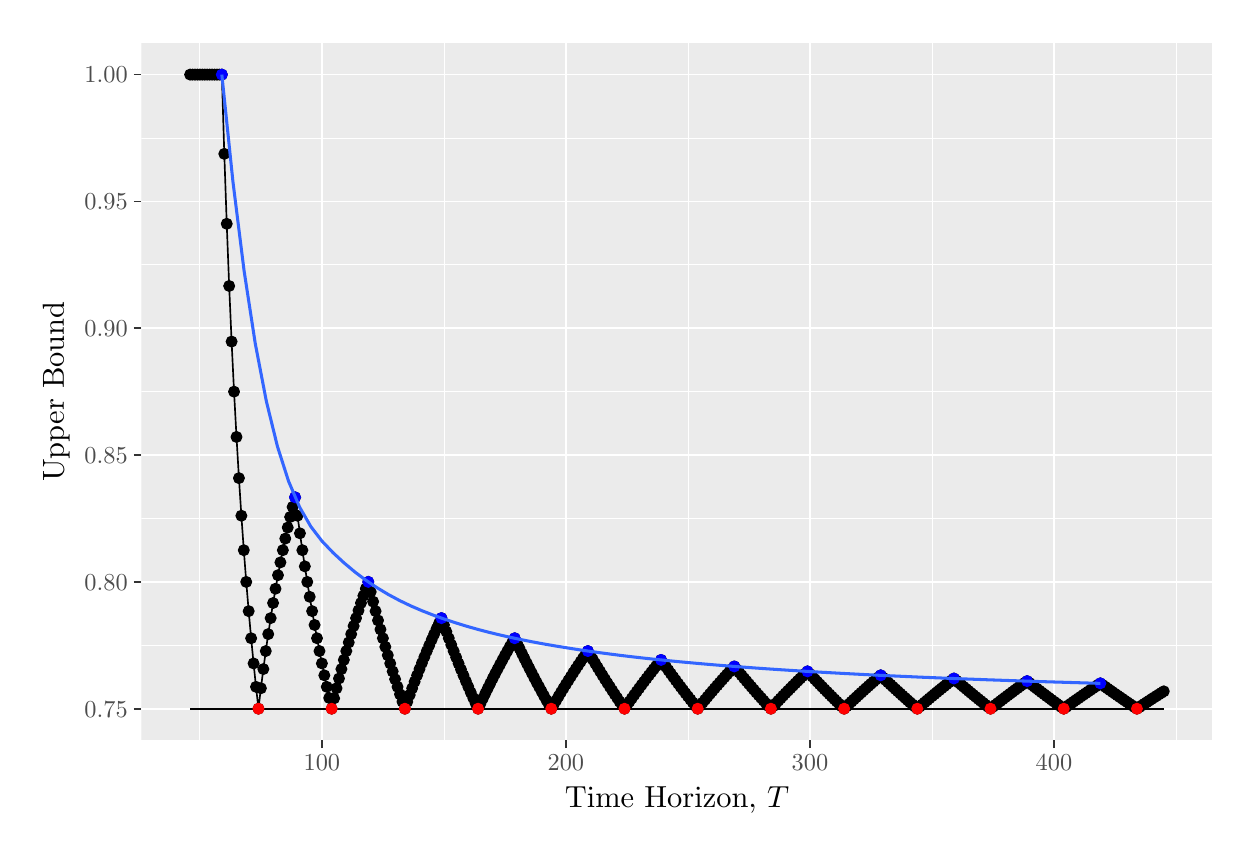
\begin{tikzpicture}[x=1pt,y=1pt]
\definecolor{fillColor}{RGB}{255,255,255}
\path[use as bounding box,fill=fillColor,fill opacity=0.00] (0,0) rectangle (433.62,289.08);
\begin{scope}
\path[clip] (  0.00,  0.00) rectangle (433.62,289.08);
\definecolor{drawColor}{RGB}{255,255,255}
\definecolor{fillColor}{RGB}{255,255,255}

\path[draw=drawColor,line width= 0.6pt,line join=round,line cap=round,fill=fillColor] (  0.00,  0.00) rectangle (433.62,289.08);
\end{scope}
\begin{scope}
\path[clip] ( 41.11, 31.53) rectangle (428.12,283.58);
\definecolor{fillColor}{gray}{0.92}

\path[fill=fillColor] ( 41.11, 31.53) rectangle (428.12,283.58);
\definecolor{drawColor}{RGB}{255,255,255}

\path[draw=drawColor,line width= 0.3pt,line join=round] ( 41.11, 65.90) --
	(428.12, 65.90);

\path[draw=drawColor,line width= 0.3pt,line join=round] ( 41.11,111.73) --
	(428.12,111.73);

\path[draw=drawColor,line width= 0.3pt,line join=round] ( 41.11,157.56) --
	(428.12,157.56);

\path[draw=drawColor,line width= 0.3pt,line join=round] ( 41.11,203.38) --
	(428.12,203.38);

\path[draw=drawColor,line width= 0.3pt,line join=round] ( 41.11,249.21) --
	(428.12,249.21);

\path[draw=drawColor,line width= 0.3pt,line join=round] ( 62.23, 31.53) --
	( 62.23,283.58);

\path[draw=drawColor,line width= 0.3pt,line join=round] (150.41, 31.53) --
	(150.41,283.58);

\path[draw=drawColor,line width= 0.3pt,line join=round] (238.58, 31.53) --
	(238.58,283.58);

\path[draw=drawColor,line width= 0.3pt,line join=round] (326.76, 31.53) --
	(326.76,283.58);

\path[draw=drawColor,line width= 0.3pt,line join=round] (414.94, 31.53) --
	(414.94,283.58);

\path[draw=drawColor,line width= 0.6pt,line join=round] ( 41.11, 42.99) --
	(428.12, 42.99);

\path[draw=drawColor,line width= 0.6pt,line join=round] ( 41.11, 88.81) --
	(428.12, 88.81);

\path[draw=drawColor,line width= 0.6pt,line join=round] ( 41.11,134.64) --
	(428.12,134.64);

\path[draw=drawColor,line width= 0.6pt,line join=round] ( 41.11,180.47) --
	(428.12,180.47);

\path[draw=drawColor,line width= 0.6pt,line join=round] ( 41.11,226.30) --
	(428.12,226.30);

\path[draw=drawColor,line width= 0.6pt,line join=round] ( 41.11,272.12) --
	(428.12,272.12);

\path[draw=drawColor,line width= 0.6pt,line join=round] (106.32, 31.53) --
	(106.32,283.58);

\path[draw=drawColor,line width= 0.6pt,line join=round] (194.49, 31.53) --
	(194.49,283.58);

\path[draw=drawColor,line width= 0.6pt,line join=round] (282.67, 31.53) --
	(282.67,283.58);

\path[draw=drawColor,line width= 0.6pt,line join=round] (370.85, 31.53) --
	(370.85,283.58);
\definecolor{drawColor}{RGB}{0,0,0}
\definecolor{fillColor}{RGB}{0,0,0}

\path[draw=drawColor,line width= 0.4pt,line join=round,line cap=round,fill=fillColor] ( 58.70,272.12) circle (  1.96);

\path[draw=drawColor,line width= 0.4pt,line join=round,line cap=round,fill=fillColor] ( 59.58,272.12) circle (  1.96);

\path[draw=drawColor,line width= 0.4pt,line join=round,line cap=round,fill=fillColor] ( 60.47,272.12) circle (  1.96);

\path[draw=drawColor,line width= 0.4pt,line join=round,line cap=round,fill=fillColor] ( 61.35,272.12) circle (  1.96);

\path[draw=drawColor,line width= 0.4pt,line join=round,line cap=round,fill=fillColor] ( 62.23,272.12) circle (  1.96);

\path[draw=drawColor,line width= 0.4pt,line join=round,line cap=round,fill=fillColor] ( 63.11,272.12) circle (  1.96);

\path[draw=drawColor,line width= 0.4pt,line join=round,line cap=round,fill=fillColor] ( 63.99,272.12) circle (  1.96);

\path[draw=drawColor,line width= 0.4pt,line join=round,line cap=round,fill=fillColor] ( 64.87,272.12) circle (  1.96);

\path[draw=drawColor,line width= 0.4pt,line join=round,line cap=round,fill=fillColor] ( 65.76,272.12) circle (  1.96);

\path[draw=drawColor,line width= 0.4pt,line join=round,line cap=round,fill=fillColor] ( 66.64,272.12) circle (  1.96);

\path[draw=drawColor,line width= 0.4pt,line join=round,line cap=round,fill=fillColor] ( 67.52,272.12) circle (  1.96);

\path[draw=drawColor,line width= 0.4pt,line join=round,line cap=round,fill=fillColor] ( 68.40,272.12) circle (  1.96);

\path[draw=drawColor,line width= 0.4pt,line join=round,line cap=round,fill=fillColor] ( 69.28,272.12) circle (  1.96);

\path[draw=drawColor,line width= 0.4pt,line join=round,line cap=round,fill=fillColor] ( 70.16,272.12) circle (  1.96);

\path[draw=drawColor,line width= 0.4pt,line join=round,line cap=round,fill=fillColor] ( 71.05,243.48) circle (  1.96);

\path[draw=drawColor,line width= 0.4pt,line join=round,line cap=round,fill=fillColor] ( 71.93,218.21) circle (  1.96);

\path[draw=drawColor,line width= 0.4pt,line join=round,line cap=round,fill=fillColor] ( 72.81,195.74) circle (  1.96);

\path[draw=drawColor,line width= 0.4pt,line join=round,line cap=round,fill=fillColor] ( 73.69,175.65) circle (  1.96);

\path[draw=drawColor,line width= 0.4pt,line join=round,line cap=round,fill=fillColor] ( 74.57,157.56) circle (  1.96);

\path[draw=drawColor,line width= 0.4pt,line join=round,line cap=round,fill=fillColor] ( 75.46,141.19) circle (  1.96);

\path[draw=drawColor,line width= 0.4pt,line join=round,line cap=round,fill=fillColor] ( 76.34,126.31) circle (  1.96);

\path[draw=drawColor,line width= 0.4pt,line join=round,line cap=round,fill=fillColor] ( 77.22,112.72) circle (  1.96);

\path[draw=drawColor,line width= 0.4pt,line join=round,line cap=round,fill=fillColor] ( 78.10,100.27) circle (  1.96);

\path[draw=drawColor,line width= 0.4pt,line join=round,line cap=round,fill=fillColor] ( 78.98, 88.81) circle (  1.96);

\path[draw=drawColor,line width= 0.4pt,line join=round,line cap=round,fill=fillColor] ( 79.86, 78.24) circle (  1.96);

\path[draw=drawColor,line width= 0.4pt,line join=round,line cap=round,fill=fillColor] ( 80.75, 68.45) circle (  1.96);

\path[draw=drawColor,line width= 0.4pt,line join=round,line cap=round,fill=fillColor] ( 81.63, 59.35) circle (  1.96);

\path[draw=drawColor,line width= 0.4pt,line join=round,line cap=round,fill=fillColor] ( 82.51, 50.89) circle (  1.96);

\path[draw=drawColor,line width= 0.4pt,line join=round,line cap=round,fill=fillColor] ( 83.39, 42.99) circle (  1.96);

\path[draw=drawColor,line width= 0.4pt,line join=round,line cap=round,fill=fillColor] ( 84.27, 50.38) circle (  1.96);

\path[draw=drawColor,line width= 0.4pt,line join=round,line cap=round,fill=fillColor] ( 85.16, 57.31) circle (  1.96);

\path[draw=drawColor,line width= 0.4pt,line join=round,line cap=round,fill=fillColor] ( 86.04, 63.82) circle (  1.96);

\path[draw=drawColor,line width= 0.4pt,line join=round,line cap=round,fill=fillColor] ( 86.92, 69.94) circle (  1.96);

\path[draw=drawColor,line width= 0.4pt,line join=round,line cap=round,fill=fillColor] ( 87.80, 75.72) circle (  1.96);

\path[draw=drawColor,line width= 0.4pt,line join=round,line cap=round,fill=fillColor] ( 88.68, 81.18) circle (  1.96);

\path[draw=drawColor,line width= 0.4pt,line join=round,line cap=round,fill=fillColor] ( 89.56, 86.34) circle (  1.96);

\path[draw=drawColor,line width= 0.4pt,line join=round,line cap=round,fill=fillColor] ( 90.45, 91.23) circle (  1.96);

\path[draw=drawColor,line width= 0.4pt,line join=round,line cap=round,fill=fillColor] ( 91.33, 95.86) circle (  1.96);

\path[draw=drawColor,line width= 0.4pt,line join=round,line cap=round,fill=fillColor] ( 92.21,100.27) circle (  1.96);

\path[draw=drawColor,line width= 0.4pt,line join=round,line cap=round,fill=fillColor] ( 93.09,104.46) circle (  1.96);

\path[draw=drawColor,line width= 0.4pt,line join=round,line cap=round,fill=fillColor] ( 93.97,108.45) circle (  1.96);

\path[draw=drawColor,line width= 0.4pt,line join=round,line cap=round,fill=fillColor] ( 94.85,112.26) circle (  1.96);

\path[draw=drawColor,line width= 0.4pt,line join=round,line cap=round,fill=fillColor] ( 95.74,115.89) circle (  1.96);

\path[draw=drawColor,line width= 0.4pt,line join=round,line cap=round,fill=fillColor] ( 96.62,119.37) circle (  1.96);

\path[draw=drawColor,line width= 0.4pt,line join=round,line cap=round,fill=fillColor] ( 97.50,112.72) circle (  1.96);

\path[draw=drawColor,line width= 0.4pt,line join=round,line cap=round,fill=fillColor] ( 98.38,106.37) circle (  1.96);

\path[draw=drawColor,line width= 0.4pt,line join=round,line cap=round,fill=fillColor] ( 99.26,100.27) circle (  1.96);

\path[draw=drawColor,line width= 0.4pt,line join=round,line cap=round,fill=fillColor] (100.15, 94.43) circle (  1.96);

\path[draw=drawColor,line width= 0.4pt,line join=round,line cap=round,fill=fillColor] (101.03, 88.81) circle (  1.96);

\path[draw=drawColor,line width= 0.4pt,line join=round,line cap=round,fill=fillColor] (101.91, 83.42) circle (  1.96);

\path[draw=drawColor,line width= 0.4pt,line join=round,line cap=round,fill=fillColor] (102.79, 78.24) circle (  1.96);

\path[draw=drawColor,line width= 0.4pt,line join=round,line cap=round,fill=fillColor] (103.67, 73.25) circle (  1.96);

\path[draw=drawColor,line width= 0.4pt,line join=round,line cap=round,fill=fillColor] (104.55, 68.45) circle (  1.96);

\path[draw=drawColor,line width= 0.4pt,line join=round,line cap=round,fill=fillColor] (105.44, 63.82) circle (  1.96);

\path[draw=drawColor,line width= 0.4pt,line join=round,line cap=round,fill=fillColor] (106.32, 59.35) circle (  1.96);

\path[draw=drawColor,line width= 0.4pt,line join=round,line cap=round,fill=fillColor] (107.20, 55.05) circle (  1.96);

\path[draw=drawColor,line width= 0.4pt,line join=round,line cap=round,fill=fillColor] (108.08, 50.89) circle (  1.96);

\path[draw=drawColor,line width= 0.4pt,line join=round,line cap=round,fill=fillColor] (108.96, 46.87) circle (  1.96);

\path[draw=drawColor,line width= 0.4pt,line join=round,line cap=round,fill=fillColor] (109.84, 42.99) circle (  1.96);

\path[draw=drawColor,line width= 0.4pt,line join=round,line cap=round,fill=fillColor] (110.73, 46.74) circle (  1.96);

\path[draw=drawColor,line width= 0.4pt,line join=round,line cap=round,fill=fillColor] (111.61, 50.38) circle (  1.96);

\path[draw=drawColor,line width= 0.4pt,line join=round,line cap=round,fill=fillColor] (112.49, 53.90) circle (  1.96);

\path[draw=drawColor,line width= 0.4pt,line join=round,line cap=round,fill=fillColor] (113.37, 57.31) circle (  1.96);

\path[draw=drawColor,line width= 0.4pt,line join=round,line cap=round,fill=fillColor] (114.25, 60.61) circle (  1.96);

\path[draw=drawColor,line width= 0.4pt,line join=round,line cap=round,fill=fillColor] (115.14, 63.82) circle (  1.96);

\path[draw=drawColor,line width= 0.4pt,line join=round,line cap=round,fill=fillColor] (116.02, 66.93) circle (  1.96);

\path[draw=drawColor,line width= 0.4pt,line join=round,line cap=round,fill=fillColor] (116.90, 69.94) circle (  1.96);

\path[draw=drawColor,line width= 0.4pt,line join=round,line cap=round,fill=fillColor] (117.78, 72.87) circle (  1.96);

\path[draw=drawColor,line width= 0.4pt,line join=round,line cap=round,fill=fillColor] (118.66, 75.72) circle (  1.96);

\path[draw=drawColor,line width= 0.4pt,line join=round,line cap=round,fill=fillColor] (119.54, 78.49) circle (  1.96);

\path[draw=drawColor,line width= 0.4pt,line join=round,line cap=round,fill=fillColor] (120.43, 81.18) circle (  1.96);

\path[draw=drawColor,line width= 0.4pt,line join=round,line cap=round,fill=fillColor] (121.31, 83.79) circle (  1.96);

\path[draw=drawColor,line width= 0.4pt,line join=round,line cap=round,fill=fillColor] (122.19, 86.34) circle (  1.96);

\path[draw=drawColor,line width= 0.4pt,line join=round,line cap=round,fill=fillColor] (123.07, 88.81) circle (  1.96);

\path[draw=drawColor,line width= 0.4pt,line join=round,line cap=round,fill=fillColor] (123.95, 85.20) circle (  1.96);

\path[draw=drawColor,line width= 0.4pt,line join=round,line cap=round,fill=fillColor] (124.83, 81.67) circle (  1.96);

\path[draw=drawColor,line width= 0.4pt,line join=round,line cap=round,fill=fillColor] (125.72, 78.24) circle (  1.96);

\path[draw=drawColor,line width= 0.4pt,line join=round,line cap=round,fill=fillColor] (126.60, 74.89) circle (  1.96);

\path[draw=drawColor,line width= 0.4pt,line join=round,line cap=round,fill=fillColor] (127.48, 71.63) circle (  1.96);

\path[draw=drawColor,line width= 0.4pt,line join=round,line cap=round,fill=fillColor] (128.36, 68.45) circle (  1.96);

\path[draw=drawColor,line width= 0.4pt,line join=round,line cap=round,fill=fillColor] (129.24, 65.34) circle (  1.96);

\path[draw=drawColor,line width= 0.4pt,line join=round,line cap=round,fill=fillColor] (130.13, 62.31) circle (  1.96);

\path[draw=drawColor,line width= 0.4pt,line join=round,line cap=round,fill=fillColor] (131.01, 59.35) circle (  1.96);

\path[draw=drawColor,line width= 0.4pt,line join=round,line cap=round,fill=fillColor] (131.89, 56.47) circle (  1.96);

\path[draw=drawColor,line width= 0.4pt,line join=round,line cap=round,fill=fillColor] (132.77, 53.64) circle (  1.96);

\path[draw=drawColor,line width= 0.4pt,line join=round,line cap=round,fill=fillColor] (133.65, 50.89) circle (  1.96);

\path[draw=drawColor,line width= 0.4pt,line join=round,line cap=round,fill=fillColor] (134.53, 48.20) circle (  1.96);

\path[draw=drawColor,line width= 0.4pt,line join=round,line cap=round,fill=fillColor] (135.42, 45.56) circle (  1.96);

\path[draw=drawColor,line width= 0.4pt,line join=round,line cap=round,fill=fillColor] (136.30, 42.99) circle (  1.96);

\path[draw=drawColor,line width= 0.4pt,line join=round,line cap=round,fill=fillColor] (137.18, 45.51) circle (  1.96);

\path[draw=drawColor,line width= 0.4pt,line join=round,line cap=round,fill=fillColor] (138.06, 47.97) circle (  1.96);

\path[draw=drawColor,line width= 0.4pt,line join=round,line cap=round,fill=fillColor] (138.94, 50.38) circle (  1.96);

\path[draw=drawColor,line width= 0.4pt,line join=round,line cap=round,fill=fillColor] (139.82, 52.74) circle (  1.96);

\path[draw=drawColor,line width= 0.4pt,line join=round,line cap=round,fill=fillColor] (140.71, 55.05) circle (  1.96);

\path[draw=drawColor,line width= 0.4pt,line join=round,line cap=round,fill=fillColor] (141.59, 57.31) circle (  1.96);

\path[draw=drawColor,line width= 0.4pt,line join=round,line cap=round,fill=fillColor] (142.47, 59.52) circle (  1.96);

\path[draw=drawColor,line width= 0.4pt,line join=round,line cap=round,fill=fillColor] (143.35, 61.69) circle (  1.96);

\path[draw=drawColor,line width= 0.4pt,line join=round,line cap=round,fill=fillColor] (144.23, 63.82) circle (  1.96);

\path[draw=drawColor,line width= 0.4pt,line join=round,line cap=round,fill=fillColor] (145.12, 65.90) circle (  1.96);

\path[draw=drawColor,line width= 0.4pt,line join=round,line cap=round,fill=fillColor] (146.00, 67.94) circle (  1.96);

\path[draw=drawColor,line width= 0.4pt,line join=round,line cap=round,fill=fillColor] (146.88, 69.94) circle (  1.96);

\path[draw=drawColor,line width= 0.4pt,line join=round,line cap=round,fill=fillColor] (147.76, 71.91) circle (  1.96);

\path[draw=drawColor,line width= 0.4pt,line join=round,line cap=round,fill=fillColor] (148.64, 73.83) circle (  1.96);

\path[draw=drawColor,line width= 0.4pt,line join=round,line cap=round,fill=fillColor] (149.52, 75.72) circle (  1.96);

\path[draw=drawColor,line width= 0.4pt,line join=round,line cap=round,fill=fillColor] (150.41, 73.25) circle (  1.96);

\path[draw=drawColor,line width= 0.4pt,line join=round,line cap=round,fill=fillColor] (151.29, 70.83) circle (  1.96);

\path[draw=drawColor,line width= 0.4pt,line join=round,line cap=round,fill=fillColor] (152.17, 68.45) circle (  1.96);

\path[draw=drawColor,line width= 0.4pt,line join=round,line cap=round,fill=fillColor] (153.05, 66.11) circle (  1.96);

\path[draw=drawColor,line width= 0.4pt,line join=round,line cap=round,fill=fillColor] (153.93, 63.82) circle (  1.96);

\path[draw=drawColor,line width= 0.4pt,line join=round,line cap=round,fill=fillColor] (154.82, 61.57) circle (  1.96);

\path[draw=drawColor,line width= 0.4pt,line join=round,line cap=round,fill=fillColor] (155.70, 59.35) circle (  1.96);

\path[draw=drawColor,line width= 0.4pt,line join=round,line cap=round,fill=fillColor] (156.58, 57.18) circle (  1.96);

\path[draw=drawColor,line width= 0.4pt,line join=round,line cap=round,fill=fillColor] (157.46, 55.05) circle (  1.96);

\path[draw=drawColor,line width= 0.4pt,line join=round,line cap=round,fill=fillColor] (158.34, 52.95) circle (  1.96);

\path[draw=drawColor,line width= 0.4pt,line join=round,line cap=round,fill=fillColor] (159.22, 50.89) circle (  1.96);

\path[draw=drawColor,line width= 0.4pt,line join=round,line cap=round,fill=fillColor] (160.11, 48.86) circle (  1.96);

\path[draw=drawColor,line width= 0.4pt,line join=round,line cap=round,fill=fillColor] (160.99, 46.87) circle (  1.96);

\path[draw=drawColor,line width= 0.4pt,line join=round,line cap=round,fill=fillColor] (161.87, 44.91) circle (  1.96);

\path[draw=drawColor,line width= 0.4pt,line join=round,line cap=round,fill=fillColor] (162.75, 42.99) circle (  1.96);

\path[draw=drawColor,line width= 0.4pt,line join=round,line cap=round,fill=fillColor] (163.63, 44.88) circle (  1.96);

\path[draw=drawColor,line width= 0.4pt,line join=round,line cap=round,fill=fillColor] (164.51, 46.74) circle (  1.96);

\path[draw=drawColor,line width= 0.4pt,line join=round,line cap=round,fill=fillColor] (165.40, 48.58) circle (  1.96);

\path[draw=drawColor,line width= 0.4pt,line join=round,line cap=round,fill=fillColor] (166.28, 50.38) circle (  1.96);

\path[draw=drawColor,line width= 0.4pt,line join=round,line cap=round,fill=fillColor] (167.16, 52.15) circle (  1.96);

\path[draw=drawColor,line width= 0.4pt,line join=round,line cap=round,fill=fillColor] (168.04, 53.90) circle (  1.96);

\path[draw=drawColor,line width= 0.4pt,line join=round,line cap=round,fill=fillColor] (168.92, 55.62) circle (  1.96);

\path[draw=drawColor,line width= 0.4pt,line join=round,line cap=round,fill=fillColor] (169.81, 57.31) circle (  1.96);

\path[draw=drawColor,line width= 0.4pt,line join=round,line cap=round,fill=fillColor] (170.69, 58.97) circle (  1.96);

\path[draw=drawColor,line width= 0.4pt,line join=round,line cap=round,fill=fillColor] (171.57, 60.61) circle (  1.96);

\path[draw=drawColor,line width= 0.4pt,line join=round,line cap=round,fill=fillColor] (172.45, 62.23) circle (  1.96);

\path[draw=drawColor,line width= 0.4pt,line join=round,line cap=round,fill=fillColor] (173.33, 63.82) circle (  1.96);

\path[draw=drawColor,line width= 0.4pt,line join=round,line cap=round,fill=fillColor] (174.21, 65.38) circle (  1.96);

\path[draw=drawColor,line width= 0.4pt,line join=round,line cap=round,fill=fillColor] (175.10, 66.93) circle (  1.96);

\path[draw=drawColor,line width= 0.4pt,line join=round,line cap=round,fill=fillColor] (175.98, 68.45) circle (  1.96);

\path[draw=drawColor,line width= 0.4pt,line join=round,line cap=round,fill=fillColor] (176.86, 66.57) circle (  1.96);

\path[draw=drawColor,line width= 0.4pt,line join=round,line cap=round,fill=fillColor] (177.74, 64.73) circle (  1.96);

\path[draw=drawColor,line width= 0.4pt,line join=round,line cap=round,fill=fillColor] (178.62, 62.91) circle (  1.96);

\path[draw=drawColor,line width= 0.4pt,line join=round,line cap=round,fill=fillColor] (179.50, 61.12) circle (  1.96);

\path[draw=drawColor,line width= 0.4pt,line join=round,line cap=round,fill=fillColor] (180.39, 59.35) circle (  1.96);

\path[draw=drawColor,line width= 0.4pt,line join=round,line cap=round,fill=fillColor] (181.27, 57.61) circle (  1.96);

\path[draw=drawColor,line width= 0.4pt,line join=round,line cap=round,fill=fillColor] (182.15, 55.90) circle (  1.96);

\path[draw=drawColor,line width= 0.4pt,line join=round,line cap=round,fill=fillColor] (183.03, 54.20) circle (  1.96);

\path[draw=drawColor,line width= 0.4pt,line join=round,line cap=round,fill=fillColor] (183.91, 52.53) circle (  1.96);

\path[draw=drawColor,line width= 0.4pt,line join=round,line cap=round,fill=fillColor] (184.80, 50.89) circle (  1.96);

\path[draw=drawColor,line width= 0.4pt,line join=round,line cap=round,fill=fillColor] (185.68, 49.27) circle (  1.96);

\path[draw=drawColor,line width= 0.4pt,line join=round,line cap=round,fill=fillColor] (186.56, 47.66) circle (  1.96);

\path[draw=drawColor,line width= 0.4pt,line join=round,line cap=round,fill=fillColor] (187.44, 46.08) circle (  1.96);

\path[draw=drawColor,line width= 0.4pt,line join=round,line cap=round,fill=fillColor] (188.32, 44.53) circle (  1.96);

\path[draw=drawColor,line width= 0.4pt,line join=round,line cap=round,fill=fillColor] (189.20, 42.99) circle (  1.96);

\path[draw=drawColor,line width= 0.4pt,line join=round,line cap=round,fill=fillColor] (190.09, 44.50) circle (  1.96);

\path[draw=drawColor,line width= 0.4pt,line join=round,line cap=round,fill=fillColor] (190.97, 46.00) circle (  1.96);

\path[draw=drawColor,line width= 0.4pt,line join=round,line cap=round,fill=fillColor] (191.85, 47.48) circle (  1.96);

\path[draw=drawColor,line width= 0.4pt,line join=round,line cap=round,fill=fillColor] (192.73, 48.94) circle (  1.96);

\path[draw=drawColor,line width= 0.4pt,line join=round,line cap=round,fill=fillColor] (193.61, 50.38) circle (  1.96);

\path[draw=drawColor,line width= 0.4pt,line join=round,line cap=round,fill=fillColor] (194.49, 51.80) circle (  1.96);

\path[draw=drawColor,line width= 0.4pt,line join=round,line cap=round,fill=fillColor] (195.38, 53.20) circle (  1.96);

\path[draw=drawColor,line width= 0.4pt,line join=round,line cap=round,fill=fillColor] (196.26, 54.59) circle (  1.96);

\path[draw=drawColor,line width= 0.4pt,line join=round,line cap=round,fill=fillColor] (197.14, 55.96) circle (  1.96);

\path[draw=drawColor,line width= 0.4pt,line join=round,line cap=round,fill=fillColor] (198.02, 57.31) circle (  1.96);

\path[draw=drawColor,line width= 0.4pt,line join=round,line cap=round,fill=fillColor] (198.90, 58.64) circle (  1.96);

\path[draw=drawColor,line width= 0.4pt,line join=round,line cap=round,fill=fillColor] (199.79, 59.96) circle (  1.96);

\path[draw=drawColor,line width= 0.4pt,line join=round,line cap=round,fill=fillColor] (200.67, 61.26) circle (  1.96);

\path[draw=drawColor,line width= 0.4pt,line join=round,line cap=round,fill=fillColor] (201.55, 62.55) circle (  1.96);

\path[draw=drawColor,line width= 0.4pt,line join=round,line cap=round,fill=fillColor] (202.43, 63.82) circle (  1.96);

\path[draw=drawColor,line width= 0.4pt,line join=round,line cap=round,fill=fillColor] (203.31, 62.31) circle (  1.96);

\path[draw=drawColor,line width= 0.4pt,line join=round,line cap=round,fill=fillColor] (204.19, 60.82) circle (  1.96);

\path[draw=drawColor,line width= 0.4pt,line join=round,line cap=round,fill=fillColor] (205.08, 59.35) circle (  1.96);

\path[draw=drawColor,line width= 0.4pt,line join=round,line cap=round,fill=fillColor] (205.96, 57.90) circle (  1.96);

\path[draw=drawColor,line width= 0.4pt,line join=round,line cap=round,fill=fillColor] (206.84, 56.47) circle (  1.96);

\path[draw=drawColor,line width= 0.4pt,line join=round,line cap=round,fill=fillColor] (207.72, 55.05) circle (  1.96);

\path[draw=drawColor,line width= 0.4pt,line join=round,line cap=round,fill=fillColor] (208.60, 53.64) circle (  1.96);

\path[draw=drawColor,line width= 0.4pt,line join=round,line cap=round,fill=fillColor] (209.48, 52.26) circle (  1.96);

\path[draw=drawColor,line width= 0.4pt,line join=round,line cap=round,fill=fillColor] (210.37, 50.89) circle (  1.96);

\path[draw=drawColor,line width= 0.4pt,line join=round,line cap=round,fill=fillColor] (211.25, 49.53) circle (  1.96);

\path[draw=drawColor,line width= 0.4pt,line join=round,line cap=round,fill=fillColor] (212.13, 48.20) circle (  1.96);

\path[draw=drawColor,line width= 0.4pt,line join=round,line cap=round,fill=fillColor] (213.01, 46.87) circle (  1.96);

\path[draw=drawColor,line width= 0.4pt,line join=round,line cap=round,fill=fillColor] (213.89, 45.56) circle (  1.96);

\path[draw=drawColor,line width= 0.4pt,line join=round,line cap=round,fill=fillColor] (214.78, 44.27) circle (  1.96);

\path[draw=drawColor,line width= 0.4pt,line join=round,line cap=round,fill=fillColor] (215.66, 42.99) circle (  1.96);

\path[draw=drawColor,line width= 0.4pt,line join=round,line cap=round,fill=fillColor] (216.54, 44.25) circle (  1.96);

\path[draw=drawColor,line width= 0.4pt,line join=round,line cap=round,fill=fillColor] (217.42, 45.51) circle (  1.96);

\path[draw=drawColor,line width= 0.4pt,line join=round,line cap=round,fill=fillColor] (218.30, 46.74) circle (  1.96);

\path[draw=drawColor,line width= 0.4pt,line join=round,line cap=round,fill=fillColor] (219.18, 47.97) circle (  1.96);

\path[draw=drawColor,line width= 0.4pt,line join=round,line cap=round,fill=fillColor] (220.07, 49.18) circle (  1.96);

\path[draw=drawColor,line width= 0.4pt,line join=round,line cap=round,fill=fillColor] (220.95, 50.38) circle (  1.96);

\path[draw=drawColor,line width= 0.4pt,line join=round,line cap=round,fill=fillColor] (221.83, 51.56) circle (  1.96);

\path[draw=drawColor,line width= 0.4pt,line join=round,line cap=round,fill=fillColor] (222.71, 52.74) circle (  1.96);

\path[draw=drawColor,line width= 0.4pt,line join=round,line cap=round,fill=fillColor] (223.59, 53.90) circle (  1.96);

\path[draw=drawColor,line width= 0.4pt,line join=round,line cap=round,fill=fillColor] (224.47, 55.05) circle (  1.96);

\path[draw=drawColor,line width= 0.4pt,line join=round,line cap=round,fill=fillColor] (225.36, 56.18) circle (  1.96);

\path[draw=drawColor,line width= 0.4pt,line join=round,line cap=round,fill=fillColor] (226.24, 57.31) circle (  1.96);

\path[draw=drawColor,line width= 0.4pt,line join=round,line cap=round,fill=fillColor] (227.12, 58.42) circle (  1.96);

\path[draw=drawColor,line width= 0.4pt,line join=round,line cap=round,fill=fillColor] (228.00, 59.52) circle (  1.96);

\path[draw=drawColor,line width= 0.4pt,line join=round,line cap=round,fill=fillColor] (228.88, 60.61) circle (  1.96);

\path[draw=drawColor,line width= 0.4pt,line join=round,line cap=round,fill=fillColor] (229.77, 59.35) circle (  1.96);

\path[draw=drawColor,line width= 0.4pt,line join=round,line cap=round,fill=fillColor] (230.65, 58.11) circle (  1.96);

\path[draw=drawColor,line width= 0.4pt,line join=round,line cap=round,fill=fillColor] (231.53, 56.87) circle (  1.96);

\path[draw=drawColor,line width= 0.4pt,line join=round,line cap=round,fill=fillColor] (232.41, 55.65) circle (  1.96);

\path[draw=drawColor,line width= 0.4pt,line join=round,line cap=round,fill=fillColor] (233.29, 54.44) circle (  1.96);

\path[draw=drawColor,line width= 0.4pt,line join=round,line cap=round,fill=fillColor] (234.17, 53.25) circle (  1.96);

\path[draw=drawColor,line width= 0.4pt,line join=round,line cap=round,fill=fillColor] (235.06, 52.06) circle (  1.96);

\path[draw=drawColor,line width= 0.4pt,line join=round,line cap=round,fill=fillColor] (235.94, 50.89) circle (  1.96);

\path[draw=drawColor,line width= 0.4pt,line join=round,line cap=round,fill=fillColor] (236.82, 49.73) circle (  1.96);

\path[draw=drawColor,line width= 0.4pt,line join=round,line cap=round,fill=fillColor] (237.70, 48.58) circle (  1.96);

\path[draw=drawColor,line width= 0.4pt,line join=round,line cap=round,fill=fillColor] (238.58, 47.44) circle (  1.96);

\path[draw=drawColor,line width= 0.4pt,line join=round,line cap=round,fill=fillColor] (239.47, 46.31) circle (  1.96);

\path[draw=drawColor,line width= 0.4pt,line join=round,line cap=round,fill=fillColor] (240.35, 45.19) circle (  1.96);

\path[draw=drawColor,line width= 0.4pt,line join=round,line cap=round,fill=fillColor] (241.23, 44.08) circle (  1.96);

\path[draw=drawColor,line width= 0.4pt,line join=round,line cap=round,fill=fillColor] (242.11, 42.99) circle (  1.96);

\path[draw=drawColor,line width= 0.4pt,line join=round,line cap=round,fill=fillColor] (242.99, 44.07) circle (  1.96);

\path[draw=drawColor,line width= 0.4pt,line join=round,line cap=round,fill=fillColor] (243.87, 45.15) circle (  1.96);

\path[draw=drawColor,line width= 0.4pt,line join=round,line cap=round,fill=fillColor] (244.76, 46.21) circle (  1.96);

\path[draw=drawColor,line width= 0.4pt,line join=round,line cap=round,fill=fillColor] (245.64, 47.27) circle (  1.96);

\path[draw=drawColor,line width= 0.4pt,line join=round,line cap=round,fill=fillColor] (246.52, 48.32) circle (  1.96);

\path[draw=drawColor,line width= 0.4pt,line join=round,line cap=round,fill=fillColor] (247.40, 49.35) circle (  1.96);

\path[draw=drawColor,line width= 0.4pt,line join=round,line cap=round,fill=fillColor] (248.28, 50.38) circle (  1.96);

\path[draw=drawColor,line width= 0.4pt,line join=round,line cap=round,fill=fillColor] (249.16, 51.40) circle (  1.96);

\path[draw=drawColor,line width= 0.4pt,line join=round,line cap=round,fill=fillColor] (250.05, 52.40) circle (  1.96);

\path[draw=drawColor,line width= 0.4pt,line join=round,line cap=round,fill=fillColor] (250.93, 53.40) circle (  1.96);

\path[draw=drawColor,line width= 0.4pt,line join=round,line cap=round,fill=fillColor] (251.81, 54.39) circle (  1.96);

\path[draw=drawColor,line width= 0.4pt,line join=round,line cap=round,fill=fillColor] (252.69, 55.37) circle (  1.96);

\path[draw=drawColor,line width= 0.4pt,line join=round,line cap=round,fill=fillColor] (253.57, 56.35) circle (  1.96);

\path[draw=drawColor,line width= 0.4pt,line join=round,line cap=round,fill=fillColor] (254.46, 57.31) circle (  1.96);

\path[draw=drawColor,line width= 0.4pt,line join=round,line cap=round,fill=fillColor] (255.34, 58.26) circle (  1.96);

\path[draw=drawColor,line width= 0.4pt,line join=round,line cap=round,fill=fillColor] (256.22, 57.18) circle (  1.96);

\path[draw=drawColor,line width= 0.4pt,line join=round,line cap=round,fill=fillColor] (257.10, 56.11) circle (  1.96);

\path[draw=drawColor,line width= 0.4pt,line join=round,line cap=round,fill=fillColor] (257.98, 55.05) circle (  1.96);

\path[draw=drawColor,line width= 0.4pt,line join=round,line cap=round,fill=fillColor] (258.86, 53.99) circle (  1.96);

\path[draw=drawColor,line width= 0.4pt,line join=round,line cap=round,fill=fillColor] (259.75, 52.95) circle (  1.96);

\path[draw=drawColor,line width= 0.4pt,line join=round,line cap=round,fill=fillColor] (260.63, 51.91) circle (  1.96);

\path[draw=drawColor,line width= 0.4pt,line join=round,line cap=round,fill=fillColor] (261.51, 50.89) circle (  1.96);

\path[draw=drawColor,line width= 0.4pt,line join=round,line cap=round,fill=fillColor] (262.39, 49.87) circle (  1.96);

\path[draw=drawColor,line width= 0.4pt,line join=round,line cap=round,fill=fillColor] (263.27, 48.86) circle (  1.96);

\path[draw=drawColor,line width= 0.4pt,line join=round,line cap=round,fill=fillColor] (264.15, 47.86) circle (  1.96);

\path[draw=drawColor,line width= 0.4pt,line join=round,line cap=round,fill=fillColor] (265.04, 46.87) circle (  1.96);

\path[draw=drawColor,line width= 0.4pt,line join=round,line cap=round,fill=fillColor] (265.92, 45.89) circle (  1.96);

\path[draw=drawColor,line width= 0.4pt,line join=round,line cap=round,fill=fillColor] (266.80, 44.91) circle (  1.96);

\path[draw=drawColor,line width= 0.4pt,line join=round,line cap=round,fill=fillColor] (267.68, 43.95) circle (  1.96);

\path[draw=drawColor,line width= 0.4pt,line join=round,line cap=round,fill=fillColor] (268.56, 42.99) circle (  1.96);

\path[draw=drawColor,line width= 0.4pt,line join=round,line cap=round,fill=fillColor] (269.45, 43.94) circle (  1.96);

\path[draw=drawColor,line width= 0.4pt,line join=round,line cap=round,fill=fillColor] (270.33, 44.88) circle (  1.96);

\path[draw=drawColor,line width= 0.4pt,line join=round,line cap=round,fill=fillColor] (271.21, 45.82) circle (  1.96);

\path[draw=drawColor,line width= 0.4pt,line join=round,line cap=round,fill=fillColor] (272.09, 46.74) circle (  1.96);

\path[draw=drawColor,line width= 0.4pt,line join=round,line cap=round,fill=fillColor] (272.97, 47.66) circle (  1.96);

\path[draw=drawColor,line width= 0.4pt,line join=round,line cap=round,fill=fillColor] (273.85, 48.58) circle (  1.96);

\path[draw=drawColor,line width= 0.4pt,line join=round,line cap=round,fill=fillColor] (274.74, 49.48) circle (  1.96);

\path[draw=drawColor,line width= 0.4pt,line join=round,line cap=round,fill=fillColor] (275.62, 50.38) circle (  1.96);

\path[draw=drawColor,line width= 0.4pt,line join=round,line cap=round,fill=fillColor] (276.50, 51.27) circle (  1.96);

\path[draw=drawColor,line width= 0.4pt,line join=round,line cap=round,fill=fillColor] (277.38, 52.15) circle (  1.96);

\path[draw=drawColor,line width= 0.4pt,line join=round,line cap=round,fill=fillColor] (278.26, 53.03) circle (  1.96);

\path[draw=drawColor,line width= 0.4pt,line join=round,line cap=round,fill=fillColor] (279.14, 53.90) circle (  1.96);

\path[draw=drawColor,line width= 0.4pt,line join=round,line cap=round,fill=fillColor] (280.03, 54.76) circle (  1.96);

\path[draw=drawColor,line width= 0.4pt,line join=round,line cap=round,fill=fillColor] (280.91, 55.62) circle (  1.96);

\path[draw=drawColor,line width= 0.4pt,line join=round,line cap=round,fill=fillColor] (281.79, 56.47) circle (  1.96);

\path[draw=drawColor,line width= 0.4pt,line join=round,line cap=round,fill=fillColor] (282.67, 55.52) circle (  1.96);

\path[draw=drawColor,line width= 0.4pt,line join=round,line cap=round,fill=fillColor] (283.55, 54.58) circle (  1.96);

\path[draw=drawColor,line width= 0.4pt,line join=round,line cap=round,fill=fillColor] (284.44, 53.64) circle (  1.96);

\path[draw=drawColor,line width= 0.4pt,line join=round,line cap=round,fill=fillColor] (285.32, 52.72) circle (  1.96);

\path[draw=drawColor,line width= 0.4pt,line join=round,line cap=round,fill=fillColor] (286.20, 51.80) circle (  1.96);

\path[draw=drawColor,line width= 0.4pt,line join=round,line cap=round,fill=fillColor] (287.08, 50.89) circle (  1.96);

\path[draw=drawColor,line width= 0.4pt,line join=round,line cap=round,fill=fillColor] (287.96, 49.98) circle (  1.96);

\path[draw=drawColor,line width= 0.4pt,line join=round,line cap=round,fill=fillColor] (288.84, 49.09) circle (  1.96);

\path[draw=drawColor,line width= 0.4pt,line join=round,line cap=round,fill=fillColor] (289.73, 48.20) circle (  1.96);

\path[draw=drawColor,line width= 0.4pt,line join=round,line cap=round,fill=fillColor] (290.61, 47.31) circle (  1.96);

\path[draw=drawColor,line width= 0.4pt,line join=round,line cap=round,fill=fillColor] (291.49, 46.43) circle (  1.96);

\path[draw=drawColor,line width= 0.4pt,line join=round,line cap=round,fill=fillColor] (292.37, 45.56) circle (  1.96);

\path[draw=drawColor,line width= 0.4pt,line join=round,line cap=round,fill=fillColor] (293.25, 44.70) circle (  1.96);

\path[draw=drawColor,line width= 0.4pt,line join=round,line cap=round,fill=fillColor] (294.13, 43.84) circle (  1.96);

\path[draw=drawColor,line width= 0.4pt,line join=round,line cap=round,fill=fillColor] (295.02, 42.99) circle (  1.96);

\path[draw=drawColor,line width= 0.4pt,line join=round,line cap=round,fill=fillColor] (295.90, 43.83) circle (  1.96);

\path[draw=drawColor,line width= 0.4pt,line join=round,line cap=round,fill=fillColor] (296.78, 44.67) circle (  1.96);

\path[draw=drawColor,line width= 0.4pt,line join=round,line cap=round,fill=fillColor] (297.66, 45.51) circle (  1.96);

\path[draw=drawColor,line width= 0.4pt,line join=round,line cap=round,fill=fillColor] (298.54, 46.33) circle (  1.96);

\path[draw=drawColor,line width= 0.4pt,line join=round,line cap=round,fill=fillColor] (299.43, 47.15) circle (  1.96);

\path[draw=drawColor,line width= 0.4pt,line join=round,line cap=round,fill=fillColor] (300.31, 47.97) circle (  1.96);

\path[draw=drawColor,line width= 0.4pt,line join=round,line cap=round,fill=fillColor] (301.19, 48.78) circle (  1.96);

\path[draw=drawColor,line width= 0.4pt,line join=round,line cap=round,fill=fillColor] (302.07, 49.58) circle (  1.96);

\path[draw=drawColor,line width= 0.4pt,line join=round,line cap=round,fill=fillColor] (302.95, 50.38) circle (  1.96);

\path[draw=drawColor,line width= 0.4pt,line join=round,line cap=round,fill=fillColor] (303.83, 51.17) circle (  1.96);

\path[draw=drawColor,line width= 0.4pt,line join=round,line cap=round,fill=fillColor] (304.72, 51.96) circle (  1.96);

\path[draw=drawColor,line width= 0.4pt,line join=round,line cap=round,fill=fillColor] (305.60, 52.74) circle (  1.96);

\path[draw=drawColor,line width= 0.4pt,line join=round,line cap=round,fill=fillColor] (306.48, 53.51) circle (  1.96);

\path[draw=drawColor,line width= 0.4pt,line join=round,line cap=round,fill=fillColor] (307.36, 54.28) circle (  1.96);

\path[draw=drawColor,line width= 0.4pt,line join=round,line cap=round,fill=fillColor] (308.24, 55.05) circle (  1.96);

\path[draw=drawColor,line width= 0.4pt,line join=round,line cap=round,fill=fillColor] (309.12, 54.20) circle (  1.96);

\path[draw=drawColor,line width= 0.4pt,line join=round,line cap=round,fill=fillColor] (310.01, 53.37) circle (  1.96);

\path[draw=drawColor,line width= 0.4pt,line join=round,line cap=round,fill=fillColor] (310.89, 52.53) circle (  1.96);

\path[draw=drawColor,line width= 0.4pt,line join=round,line cap=round,fill=fillColor] (311.77, 51.71) circle (  1.96);

\path[draw=drawColor,line width= 0.4pt,line join=round,line cap=round,fill=fillColor] (312.65, 50.89) circle (  1.96);

\path[draw=drawColor,line width= 0.4pt,line join=round,line cap=round,fill=fillColor] (313.53, 50.07) circle (  1.96);

\path[draw=drawColor,line width= 0.4pt,line join=round,line cap=round,fill=fillColor] (314.42, 49.27) circle (  1.96);

\path[draw=drawColor,line width= 0.4pt,line join=round,line cap=round,fill=fillColor] (315.30, 48.46) circle (  1.96);

\path[draw=drawColor,line width= 0.4pt,line join=round,line cap=round,fill=fillColor] (316.18, 47.66) circle (  1.96);

\path[draw=drawColor,line width= 0.4pt,line join=round,line cap=round,fill=fillColor] (317.06, 46.87) circle (  1.96);

\path[draw=drawColor,line width= 0.4pt,line join=round,line cap=round,fill=fillColor] (317.94, 46.08) circle (  1.96);

\path[draw=drawColor,line width= 0.4pt,line join=round,line cap=round,fill=fillColor] (318.82, 45.30) circle (  1.96);

\path[draw=drawColor,line width= 0.4pt,line join=round,line cap=round,fill=fillColor] (319.71, 44.53) circle (  1.96);

\path[draw=drawColor,line width= 0.4pt,line join=round,line cap=round,fill=fillColor] (320.59, 43.75) circle (  1.96);

\path[draw=drawColor,line width= 0.4pt,line join=round,line cap=round,fill=fillColor] (321.47, 42.99) circle (  1.96);

\path[draw=drawColor,line width= 0.4pt,line join=round,line cap=round,fill=fillColor] (322.35, 43.75) circle (  1.96);

\path[draw=drawColor,line width= 0.4pt,line join=round,line cap=round,fill=fillColor] (323.23, 44.50) circle (  1.96);

\path[draw=drawColor,line width= 0.4pt,line join=round,line cap=round,fill=fillColor] (324.12, 45.26) circle (  1.96);

\path[draw=drawColor,line width= 0.4pt,line join=round,line cap=round,fill=fillColor] (325.00, 46.00) circle (  1.96);

\path[draw=drawColor,line width= 0.4pt,line join=round,line cap=round,fill=fillColor] (325.88, 46.74) circle (  1.96);

\path[draw=drawColor,line width= 0.4pt,line join=round,line cap=round,fill=fillColor] (326.76, 47.48) circle (  1.96);

\path[draw=drawColor,line width= 0.4pt,line join=round,line cap=round,fill=fillColor] (327.64, 48.21) circle (  1.96);

\path[draw=drawColor,line width= 0.4pt,line join=round,line cap=round,fill=fillColor] (328.52, 48.94) circle (  1.96);

\path[draw=drawColor,line width= 0.4pt,line join=round,line cap=round,fill=fillColor] (329.41, 49.66) circle (  1.96);

\path[draw=drawColor,line width= 0.4pt,line join=round,line cap=round,fill=fillColor] (330.29, 50.38) circle (  1.96);

\path[draw=drawColor,line width= 0.4pt,line join=round,line cap=round,fill=fillColor] (331.17, 51.09) circle (  1.96);

\path[draw=drawColor,line width= 0.4pt,line join=round,line cap=round,fill=fillColor] (332.05, 51.80) circle (  1.96);

\path[draw=drawColor,line width= 0.4pt,line join=round,line cap=round,fill=fillColor] (332.93, 52.50) circle (  1.96);

\path[draw=drawColor,line width= 0.4pt,line join=round,line cap=round,fill=fillColor] (333.81, 53.20) circle (  1.96);

\path[draw=drawColor,line width= 0.4pt,line join=round,line cap=round,fill=fillColor] (334.70, 53.90) circle (  1.96);

\path[draw=drawColor,line width= 0.4pt,line join=round,line cap=round,fill=fillColor] (335.58, 53.14) circle (  1.96);

\path[draw=drawColor,line width= 0.4pt,line join=round,line cap=round,fill=fillColor] (336.46, 52.38) circle (  1.96);

\path[draw=drawColor,line width= 0.4pt,line join=round,line cap=round,fill=fillColor] (337.34, 51.63) circle (  1.96);

\path[draw=drawColor,line width= 0.4pt,line join=round,line cap=round,fill=fillColor] (338.22, 50.89) circle (  1.96);

\path[draw=drawColor,line width= 0.4pt,line join=round,line cap=round,fill=fillColor] (339.11, 50.15) circle (  1.96);

\path[draw=drawColor,line width= 0.4pt,line join=round,line cap=round,fill=fillColor] (339.99, 49.41) circle (  1.96);

\path[draw=drawColor,line width= 0.4pt,line join=round,line cap=round,fill=fillColor] (340.87, 48.68) circle (  1.96);

\path[draw=drawColor,line width= 0.4pt,line join=round,line cap=round,fill=fillColor] (341.75, 47.95) circle (  1.96);

\path[draw=drawColor,line width= 0.4pt,line join=round,line cap=round,fill=fillColor] (342.63, 47.23) circle (  1.96);

\path[draw=drawColor,line width= 0.4pt,line join=round,line cap=round,fill=fillColor] (343.51, 46.51) circle (  1.96);

\path[draw=drawColor,line width= 0.4pt,line join=round,line cap=round,fill=fillColor] (344.40, 45.80) circle (  1.96);

\path[draw=drawColor,line width= 0.4pt,line join=round,line cap=round,fill=fillColor] (345.28, 45.09) circle (  1.96);

\path[draw=drawColor,line width= 0.4pt,line join=round,line cap=round,fill=fillColor] (346.16, 44.38) circle (  1.96);

\path[draw=drawColor,line width= 0.4pt,line join=round,line cap=round,fill=fillColor] (347.04, 43.68) circle (  1.96);

\path[draw=drawColor,line width= 0.4pt,line join=round,line cap=round,fill=fillColor] (347.92, 42.99) circle (  1.96);

\path[draw=drawColor,line width= 0.4pt,line join=round,line cap=round,fill=fillColor] (348.80, 43.68) circle (  1.96);

\path[draw=drawColor,line width= 0.4pt,line join=round,line cap=round,fill=fillColor] (349.69, 44.37) circle (  1.96);

\path[draw=drawColor,line width= 0.4pt,line join=round,line cap=round,fill=fillColor] (350.57, 45.05) circle (  1.96);

\path[draw=drawColor,line width= 0.4pt,line join=round,line cap=round,fill=fillColor] (351.45, 45.73) circle (  1.96);

\path[draw=drawColor,line width= 0.4pt,line join=round,line cap=round,fill=fillColor] (352.33, 46.41) circle (  1.96);

\path[draw=drawColor,line width= 0.4pt,line join=round,line cap=round,fill=fillColor] (353.21, 47.08) circle (  1.96);

\path[draw=drawColor,line width= 0.4pt,line join=round,line cap=round,fill=fillColor] (354.10, 47.75) circle (  1.96);

\path[draw=drawColor,line width= 0.4pt,line join=round,line cap=round,fill=fillColor] (354.98, 48.41) circle (  1.96);

\path[draw=drawColor,line width= 0.4pt,line join=round,line cap=round,fill=fillColor] (355.86, 49.07) circle (  1.96);

\path[draw=drawColor,line width= 0.4pt,line join=round,line cap=round,fill=fillColor] (356.74, 49.73) circle (  1.96);

\path[draw=drawColor,line width= 0.4pt,line join=round,line cap=round,fill=fillColor] (357.62, 50.38) circle (  1.96);

\path[draw=drawColor,line width= 0.4pt,line join=round,line cap=round,fill=fillColor] (358.50, 51.03) circle (  1.96);

\path[draw=drawColor,line width= 0.4pt,line join=round,line cap=round,fill=fillColor] (359.39, 51.67) circle (  1.96);

\path[draw=drawColor,line width= 0.4pt,line join=round,line cap=round,fill=fillColor] (360.27, 52.31) circle (  1.96);

\path[draw=drawColor,line width= 0.4pt,line join=round,line cap=round,fill=fillColor] (361.15, 52.95) circle (  1.96);

\path[draw=drawColor,line width= 0.4pt,line join=round,line cap=round,fill=fillColor] (362.03, 52.26) circle (  1.96);

\path[draw=drawColor,line width= 0.4pt,line join=round,line cap=round,fill=fillColor] (362.91, 51.57) circle (  1.96);

\path[draw=drawColor,line width= 0.4pt,line join=round,line cap=round,fill=fillColor] (363.79, 50.89) circle (  1.96);

\path[draw=drawColor,line width= 0.4pt,line join=round,line cap=round,fill=fillColor] (364.68, 50.21) circle (  1.96);

\path[draw=drawColor,line width= 0.4pt,line join=round,line cap=round,fill=fillColor] (365.56, 49.53) circle (  1.96);

\path[draw=drawColor,line width= 0.4pt,line join=round,line cap=round,fill=fillColor] (366.44, 48.86) circle (  1.96);

\path[draw=drawColor,line width= 0.4pt,line join=round,line cap=round,fill=fillColor] (367.32, 48.20) circle (  1.96);

\path[draw=drawColor,line width= 0.4pt,line join=round,line cap=round,fill=fillColor] (368.20, 47.53) circle (  1.96);

\path[draw=drawColor,line width= 0.4pt,line join=round,line cap=round,fill=fillColor] (369.09, 46.87) circle (  1.96);

\path[draw=drawColor,line width= 0.4pt,line join=round,line cap=round,fill=fillColor] (369.97, 46.21) circle (  1.96);

\path[draw=drawColor,line width= 0.4pt,line join=round,line cap=round,fill=fillColor] (370.85, 45.56) circle (  1.96);

\path[draw=drawColor,line width= 0.4pt,line join=round,line cap=round,fill=fillColor] (371.73, 44.91) circle (  1.96);

\path[draw=drawColor,line width= 0.4pt,line join=round,line cap=round,fill=fillColor] (372.61, 44.27) circle (  1.96);

\path[draw=drawColor,line width= 0.4pt,line join=round,line cap=round,fill=fillColor] (373.49, 43.63) circle (  1.96);

\path[draw=drawColor,line width= 0.4pt,line join=round,line cap=round,fill=fillColor] (374.38, 42.99) circle (  1.96);

\path[draw=drawColor,line width= 0.4pt,line join=round,line cap=round,fill=fillColor] (375.26, 43.62) circle (  1.96);

\path[draw=drawColor,line width= 0.4pt,line join=round,line cap=round,fill=fillColor] (376.14, 44.25) circle (  1.96);

\path[draw=drawColor,line width= 0.4pt,line join=round,line cap=round,fill=fillColor] (377.02, 44.88) circle (  1.96);

\path[draw=drawColor,line width= 0.4pt,line join=round,line cap=round,fill=fillColor] (377.90, 45.51) circle (  1.96);

\path[draw=drawColor,line width= 0.4pt,line join=round,line cap=round,fill=fillColor] (378.78, 46.13) circle (  1.96);

\path[draw=drawColor,line width= 0.4pt,line join=round,line cap=round,fill=fillColor] (379.67, 46.74) circle (  1.96);

\path[draw=drawColor,line width= 0.4pt,line join=round,line cap=round,fill=fillColor] (380.55, 47.36) circle (  1.96);

\path[draw=drawColor,line width= 0.4pt,line join=round,line cap=round,fill=fillColor] (381.43, 47.97) circle (  1.96);

\path[draw=drawColor,line width= 0.4pt,line join=round,line cap=round,fill=fillColor] (382.31, 48.58) circle (  1.96);

\path[draw=drawColor,line width= 0.4pt,line join=round,line cap=round,fill=fillColor] (383.19, 49.18) circle (  1.96);

\path[draw=drawColor,line width= 0.4pt,line join=round,line cap=round,fill=fillColor] (384.08, 49.78) circle (  1.96);

\path[draw=drawColor,line width= 0.4pt,line join=round,line cap=round,fill=fillColor] (384.96, 50.38) circle (  1.96);

\path[draw=drawColor,line width= 0.4pt,line join=round,line cap=round,fill=fillColor] (385.84, 50.97) circle (  1.96);

\path[draw=drawColor,line width= 0.4pt,line join=round,line cap=round,fill=fillColor] (386.72, 51.56) circle (  1.96);

\path[draw=drawColor,line width= 0.4pt,line join=round,line cap=round,fill=fillColor] (387.60, 52.15) circle (  1.96);

\path[draw=drawColor,line width= 0.4pt,line join=round,line cap=round,fill=fillColor] (388.48, 51.52) circle (  1.96);

\path[draw=drawColor,line width= 0.4pt,line join=round,line cap=round,fill=fillColor] (389.37, 50.89) circle (  1.96);

\path[draw=drawColor,line width= 0.4pt,line join=round,line cap=round,fill=fillColor] (390.25, 50.26) circle (  1.96);

\path[draw=drawColor,line width= 0.4pt,line join=round,line cap=round,fill=fillColor] (391.13, 49.64) circle (  1.96);

\path[draw=drawColor,line width= 0.4pt,line join=round,line cap=round,fill=fillColor] (392.01, 49.02) circle (  1.96);

\path[draw=drawColor,line width= 0.4pt,line join=round,line cap=round,fill=fillColor] (392.89, 48.40) circle (  1.96);

\path[draw=drawColor,line width= 0.4pt,line join=round,line cap=round,fill=fillColor] (393.78, 47.79) circle (  1.96);

\path[draw=drawColor,line width= 0.4pt,line join=round,line cap=round,fill=fillColor] (394.66, 47.18) circle (  1.96);

\path[draw=drawColor,line width= 0.4pt,line join=round,line cap=round,fill=fillColor] (395.54, 46.57) circle (  1.96);

\path[draw=drawColor,line width= 0.4pt,line join=round,line cap=round,fill=fillColor] (396.42, 45.96) circle (  1.96);

\path[draw=drawColor,line width= 0.4pt,line join=round,line cap=round,fill=fillColor] (397.30, 45.36) circle (  1.96);

\path[draw=drawColor,line width= 0.4pt,line join=round,line cap=round,fill=fillColor] (398.18, 44.76) circle (  1.96);

\path[draw=drawColor,line width= 0.4pt,line join=round,line cap=round,fill=fillColor] (399.07, 44.17) circle (  1.96);

\path[draw=drawColor,line width= 0.4pt,line join=round,line cap=round,fill=fillColor] (399.95, 43.58) circle (  1.96);

\path[draw=drawColor,line width= 0.4pt,line join=round,line cap=round,fill=fillColor] (400.83, 42.99) circle (  1.96);

\path[draw=drawColor,line width= 0.4pt,line join=round,line cap=round,fill=fillColor] (401.71, 43.57) circle (  1.96);

\path[draw=drawColor,line width= 0.4pt,line join=round,line cap=round,fill=fillColor] (402.59, 44.16) circle (  1.96);

\path[draw=drawColor,line width= 0.4pt,line join=round,line cap=round,fill=fillColor] (403.47, 44.74) circle (  1.96);

\path[draw=drawColor,line width= 0.4pt,line join=round,line cap=round,fill=fillColor] (404.36, 45.31) circle (  1.96);

\path[draw=drawColor,line width= 0.4pt,line join=round,line cap=round,fill=fillColor] (405.24, 45.89) circle (  1.96);

\path[draw=drawColor,line width= 0.4pt,line join=round,line cap=round,fill=fillColor] (406.12, 46.46) circle (  1.96);

\path[draw=drawColor,line width= 0.4pt,line join=round,line cap=round,fill=fillColor] (407.00, 47.03) circle (  1.96);

\path[draw=drawColor,line width= 0.4pt,line join=round,line cap=round,fill=fillColor] (407.88, 47.59) circle (  1.96);

\path[draw=drawColor,line width= 0.4pt,line join=round,line cap=round,fill=fillColor] (408.77, 48.16) circle (  1.96);

\path[draw=drawColor,line width= 0.4pt,line join=round,line cap=round,fill=fillColor] (409.65, 48.72) circle (  1.96);

\path[draw=drawColor,line width= 0.4pt,line join=round,line cap=round,fill=fillColor] (410.53, 49.27) circle (  1.96);

\path[draw=drawColor,line width= 0.6pt,line join=round] ( 58.70,272.12) --
	( 59.58,272.12) --
	( 60.47,272.12) --
	( 61.35,272.12) --
	( 62.23,272.12) --
	( 63.11,272.12) --
	( 63.99,272.12) --
	( 64.87,272.12) --
	( 65.76,272.12) --
	( 66.64,272.12) --
	( 67.52,272.12) --
	( 68.40,272.12) --
	( 69.28,272.12) --
	( 70.16,272.12) --
	( 71.05,243.48) --
	( 71.93,218.21) --
	( 72.81,195.74) --
	( 73.69,175.65) --
	( 74.57,157.56) --
	( 75.46,141.19) --
	( 76.34,126.31) --
	( 77.22,112.72) --
	( 78.10,100.27) --
	( 78.98, 88.81) --
	( 79.86, 78.24) --
	( 80.75, 68.45) --
	( 81.63, 59.35) --
	( 82.51, 50.89) --
	( 83.39, 42.99) --
	( 84.27, 50.38) --
	( 85.16, 57.31) --
	( 86.04, 63.82) --
	( 86.92, 69.94) --
	( 87.80, 75.72) --
	( 88.68, 81.18) --
	( 89.56, 86.34) --
	( 90.45, 91.23) --
	( 91.33, 95.86) --
	( 92.21,100.27) --
	( 93.09,104.46) --
	( 93.97,108.45) --
	( 94.85,112.26) --
	( 95.74,115.89) --
	( 96.62,119.37) --
	( 97.50,112.72) --
	( 98.38,106.37) --
	( 99.26,100.27) --
	(100.15, 94.43) --
	(101.03, 88.81) --
	(101.91, 83.42) --
	(102.79, 78.24) --
	(103.67, 73.25) --
	(104.55, 68.45) --
	(105.44, 63.82) --
	(106.32, 59.35) --
	(107.20, 55.05) --
	(108.08, 50.89) --
	(108.96, 46.87) --
	(109.84, 42.99) --
	(110.73, 46.74) --
	(111.61, 50.38) --
	(112.49, 53.90) --
	(113.37, 57.31) --
	(114.25, 60.61) --
	(115.14, 63.82) --
	(116.02, 66.93) --
	(116.90, 69.94) --
	(117.78, 72.87) --
	(118.66, 75.72) --
	(119.54, 78.49) --
	(120.43, 81.18) --
	(121.31, 83.79) --
	(122.19, 86.34) --
	(123.07, 88.81) --
	(123.95, 85.20) --
	(124.83, 81.67) --
	(125.72, 78.24) --
	(126.60, 74.89) --
	(127.48, 71.63) --
	(128.36, 68.45) --
	(129.24, 65.34) --
	(130.13, 62.31) --
	(131.01, 59.35) --
	(131.89, 56.47) --
	(132.77, 53.64) --
	(133.65, 50.89) --
	(134.53, 48.20) --
	(135.42, 45.56) --
	(136.30, 42.99) --
	(137.18, 45.51) --
	(138.06, 47.97) --
	(138.94, 50.38) --
	(139.82, 52.74) --
	(140.71, 55.05) --
	(141.59, 57.31) --
	(142.47, 59.52) --
	(143.35, 61.69) --
	(144.23, 63.82) --
	(145.12, 65.90) --
	(146.00, 67.94) --
	(146.88, 69.94) --
	(147.76, 71.91) --
	(148.64, 73.83) --
	(149.52, 75.72) --
	(150.41, 73.25) --
	(151.29, 70.83) --
	(152.17, 68.45) --
	(153.05, 66.11) --
	(153.93, 63.82) --
	(154.82, 61.57) --
	(155.70, 59.35) --
	(156.58, 57.18) --
	(157.46, 55.05) --
	(158.34, 52.95) --
	(159.22, 50.89) --
	(160.11, 48.86) --
	(160.99, 46.87) --
	(161.87, 44.91) --
	(162.75, 42.99) --
	(163.63, 44.88) --
	(164.51, 46.74) --
	(165.40, 48.58) --
	(166.28, 50.38) --
	(167.16, 52.15) --
	(168.04, 53.90) --
	(168.92, 55.62) --
	(169.81, 57.31) --
	(170.69, 58.97) --
	(171.57, 60.61) --
	(172.45, 62.23) --
	(173.33, 63.82) --
	(174.21, 65.38) --
	(175.10, 66.93) --
	(175.98, 68.45) --
	(176.86, 66.57) --
	(177.74, 64.73) --
	(178.62, 62.91) --
	(179.50, 61.12) --
	(180.39, 59.35) --
	(181.27, 57.61) --
	(182.15, 55.90) --
	(183.03, 54.20) --
	(183.91, 52.53) --
	(184.80, 50.89) --
	(185.68, 49.27) --
	(186.56, 47.66) --
	(187.44, 46.08) --
	(188.32, 44.53) --
	(189.20, 42.99) --
	(190.09, 44.50) --
	(190.97, 46.00) --
	(191.85, 47.48) --
	(192.73, 48.94) --
	(193.61, 50.38) --
	(194.49, 51.80) --
	(195.38, 53.20) --
	(196.26, 54.59) --
	(197.14, 55.96) --
	(198.02, 57.31) --
	(198.90, 58.64) --
	(199.79, 59.96) --
	(200.67, 61.26) --
	(201.55, 62.55) --
	(202.43, 63.82) --
	(203.31, 62.31) --
	(204.19, 60.82) --
	(205.08, 59.35) --
	(205.96, 57.90) --
	(206.84, 56.47) --
	(207.72, 55.05) --
	(208.60, 53.64) --
	(209.48, 52.26) --
	(210.37, 50.89) --
	(211.25, 49.53) --
	(212.13, 48.20) --
	(213.01, 46.87) --
	(213.89, 45.56) --
	(214.78, 44.27) --
	(215.66, 42.99) --
	(216.54, 44.25) --
	(217.42, 45.51) --
	(218.30, 46.74) --
	(219.18, 47.97) --
	(220.07, 49.18) --
	(220.95, 50.38) --
	(221.83, 51.56) --
	(222.71, 52.74) --
	(223.59, 53.90) --
	(224.47, 55.05) --
	(225.36, 56.18) --
	(226.24, 57.31) --
	(227.12, 58.42) --
	(228.00, 59.52) --
	(228.88, 60.61) --
	(229.77, 59.35) --
	(230.65, 58.11) --
	(231.53, 56.87) --
	(232.41, 55.65) --
	(233.29, 54.44) --
	(234.17, 53.25) --
	(235.06, 52.06) --
	(235.94, 50.89) --
	(236.82, 49.73) --
	(237.70, 48.58) --
	(238.58, 47.44) --
	(239.47, 46.31) --
	(240.35, 45.19) --
	(241.23, 44.08) --
	(242.11, 42.99) --
	(242.99, 44.07) --
	(243.87, 45.15) --
	(244.76, 46.21) --
	(245.64, 47.27) --
	(246.52, 48.32) --
	(247.40, 49.35) --
	(248.28, 50.38) --
	(249.16, 51.40) --
	(250.05, 52.40) --
	(250.93, 53.40) --
	(251.81, 54.39) --
	(252.69, 55.37) --
	(253.57, 56.35) --
	(254.46, 57.31) --
	(255.34, 58.26) --
	(256.22, 57.18) --
	(257.10, 56.11) --
	(257.98, 55.05) --
	(258.86, 53.99) --
	(259.75, 52.95) --
	(260.63, 51.91) --
	(261.51, 50.89) --
	(262.39, 49.87) --
	(263.27, 48.86) --
	(264.15, 47.86) --
	(265.04, 46.87) --
	(265.92, 45.89) --
	(266.80, 44.91) --
	(267.68, 43.95) --
	(268.56, 42.99) --
	(269.45, 43.94) --
	(270.33, 44.88) --
	(271.21, 45.82) --
	(272.09, 46.74) --
	(272.97, 47.66) --
	(273.85, 48.58) --
	(274.74, 49.48) --
	(275.62, 50.38) --
	(276.50, 51.27) --
	(277.38, 52.15) --
	(278.26, 53.03) --
	(279.14, 53.90) --
	(280.03, 54.76) --
	(280.91, 55.62) --
	(281.79, 56.47) --
	(282.67, 55.52) --
	(283.55, 54.58) --
	(284.44, 53.64) --
	(285.32, 52.72) --
	(286.20, 51.80) --
	(287.08, 50.89) --
	(287.96, 49.98) --
	(288.84, 49.09) --
	(289.73, 48.20) --
	(290.61, 47.31) --
	(291.49, 46.43) --
	(292.37, 45.56) --
	(293.25, 44.70) --
	(294.13, 43.84) --
	(295.02, 42.99) --
	(295.90, 43.83) --
	(296.78, 44.67) --
	(297.66, 45.51) --
	(298.54, 46.33) --
	(299.43, 47.15) --
	(300.31, 47.97) --
	(301.19, 48.78) --
	(302.07, 49.58) --
	(302.95, 50.38) --
	(303.83, 51.17) --
	(304.72, 51.96) --
	(305.60, 52.74) --
	(306.48, 53.51) --
	(307.36, 54.28) --
	(308.24, 55.05) --
	(309.12, 54.20) --
	(310.01, 53.37) --
	(310.89, 52.53) --
	(311.77, 51.71) --
	(312.65, 50.89) --
	(313.53, 50.07) --
	(314.42, 49.27) --
	(315.30, 48.46) --
	(316.18, 47.66) --
	(317.06, 46.87) --
	(317.94, 46.08) --
	(318.82, 45.30) --
	(319.71, 44.53) --
	(320.59, 43.75) --
	(321.47, 42.99) --
	(322.35, 43.75) --
	(323.23, 44.50) --
	(324.12, 45.26) --
	(325.00, 46.00) --
	(325.88, 46.74) --
	(326.76, 47.48) --
	(327.64, 48.21) --
	(328.52, 48.94) --
	(329.41, 49.66) --
	(330.29, 50.38) --
	(331.17, 51.09) --
	(332.05, 51.80) --
	(332.93, 52.50) --
	(333.81, 53.20) --
	(334.70, 53.90) --
	(335.58, 53.14) --
	(336.46, 52.38) --
	(337.34, 51.63) --
	(338.22, 50.89) --
	(339.11, 50.15) --
	(339.99, 49.41) --
	(340.87, 48.68) --
	(341.75, 47.95) --
	(342.63, 47.23) --
	(343.51, 46.51) --
	(344.40, 45.80) --
	(345.28, 45.09) --
	(346.16, 44.38) --
	(347.04, 43.68) --
	(347.92, 42.99) --
	(348.80, 43.68) --
	(349.69, 44.37) --
	(350.57, 45.05) --
	(351.45, 45.73) --
	(352.33, 46.41) --
	(353.21, 47.08) --
	(354.10, 47.75) --
	(354.98, 48.41) --
	(355.86, 49.07) --
	(356.74, 49.73) --
	(357.62, 50.38) --
	(358.50, 51.03) --
	(359.39, 51.67) --
	(360.27, 52.31) --
	(361.15, 52.95) --
	(362.03, 52.26) --
	(362.91, 51.57) --
	(363.79, 50.89) --
	(364.68, 50.21) --
	(365.56, 49.53) --
	(366.44, 48.86) --
	(367.32, 48.20) --
	(368.20, 47.53) --
	(369.09, 46.87) --
	(369.97, 46.21) --
	(370.85, 45.56) --
	(371.73, 44.91) --
	(372.61, 44.27) --
	(373.49, 43.63) --
	(374.38, 42.99) --
	(375.26, 43.62) --
	(376.14, 44.25) --
	(377.02, 44.88) --
	(377.90, 45.51) --
	(378.78, 46.13) --
	(379.67, 46.74) --
	(380.55, 47.36) --
	(381.43, 47.97) --
	(382.31, 48.58) --
	(383.19, 49.18) --
	(384.08, 49.78) --
	(384.96, 50.38) --
	(385.84, 50.97) --
	(386.72, 51.56) --
	(387.60, 52.15) --
	(388.48, 51.52) --
	(389.37, 50.89) --
	(390.25, 50.26) --
	(391.13, 49.64) --
	(392.01, 49.02) --
	(392.89, 48.40) --
	(393.78, 47.79) --
	(394.66, 47.18) --
	(395.54, 46.57) --
	(396.42, 45.96) --
	(397.30, 45.36) --
	(398.18, 44.76) --
	(399.07, 44.17) --
	(399.95, 43.58) --
	(400.83, 42.99) --
	(401.71, 43.57) --
	(402.59, 44.16) --
	(403.47, 44.74) --
	(404.36, 45.31) --
	(405.24, 45.89) --
	(406.12, 46.46) --
	(407.00, 47.03) --
	(407.88, 47.59) --
	(408.77, 48.16) --
	(409.65, 48.72) --
	(410.53, 49.27);

\path[draw=drawColor,line width= 0.6pt,line join=round] ( 58.70, 42.99) --
	( 59.58, 42.99) --
	( 60.47, 42.99) --
	( 61.35, 42.99) --
	( 62.23, 42.99) --
	( 63.11, 42.99) --
	( 63.99, 42.99) --
	( 64.87, 42.99) --
	( 65.76, 42.99) --
	( 66.64, 42.99) --
	( 67.52, 42.99) --
	( 68.40, 42.99) --
	( 69.28, 42.99) --
	( 70.16, 42.99) --
	( 71.05, 42.99) --
	( 71.93, 42.99) --
	( 72.81, 42.99) --
	( 73.69, 42.99) --
	( 74.57, 42.99) --
	( 75.46, 42.99) --
	( 76.34, 42.99) --
	( 77.22, 42.99) --
	( 78.10, 42.99) --
	( 78.98, 42.99) --
	( 79.86, 42.99) --
	( 80.75, 42.99) --
	( 81.63, 42.99) --
	( 82.51, 42.99) --
	( 83.39, 42.99) --
	( 84.27, 42.99) --
	( 85.16, 42.99) --
	( 86.04, 42.99) --
	( 86.92, 42.99) --
	( 87.80, 42.99) --
	( 88.68, 42.99) --
	( 89.56, 42.99) --
	( 90.45, 42.99) --
	( 91.33, 42.99) --
	( 92.21, 42.99) --
	( 93.09, 42.99) --
	( 93.97, 42.99) --
	( 94.85, 42.99) --
	( 95.74, 42.99) --
	( 96.62, 42.99) --
	( 97.50, 42.99) --
	( 98.38, 42.99) --
	( 99.26, 42.99) --
	(100.15, 42.99) --
	(101.03, 42.99) --
	(101.91, 42.99) --
	(102.79, 42.99) --
	(103.67, 42.99) --
	(104.55, 42.99) --
	(105.44, 42.99) --
	(106.32, 42.99) --
	(107.20, 42.99) --
	(108.08, 42.99) --
	(108.96, 42.99) --
	(109.84, 42.99) --
	(110.73, 42.99) --
	(111.61, 42.99) --
	(112.49, 42.99) --
	(113.37, 42.99) --
	(114.25, 42.99) --
	(115.14, 42.99) --
	(116.02, 42.99) --
	(116.90, 42.99) --
	(117.78, 42.99) --
	(118.66, 42.99) --
	(119.54, 42.99) --
	(120.43, 42.99) --
	(121.31, 42.99) --
	(122.19, 42.99) --
	(123.07, 42.99) --
	(123.95, 42.99) --
	(124.83, 42.99) --
	(125.72, 42.99) --
	(126.60, 42.99) --
	(127.48, 42.99) --
	(128.36, 42.99) --
	(129.24, 42.99) --
	(130.13, 42.99) --
	(131.01, 42.99) --
	(131.89, 42.99) --
	(132.77, 42.99) --
	(133.65, 42.99) --
	(134.53, 42.99) --
	(135.42, 42.99) --
	(136.30, 42.99) --
	(137.18, 42.99) --
	(138.06, 42.99) --
	(138.94, 42.99) --
	(139.82, 42.99) --
	(140.71, 42.99) --
	(141.59, 42.99) --
	(142.47, 42.99) --
	(143.35, 42.99) --
	(144.23, 42.99) --
	(145.12, 42.99) --
	(146.00, 42.99) --
	(146.88, 42.99) --
	(147.76, 42.99) --
	(148.64, 42.99) --
	(149.52, 42.99) --
	(150.41, 42.99) --
	(151.29, 42.99) --
	(152.17, 42.99) --
	(153.05, 42.99) --
	(153.93, 42.99) --
	(154.82, 42.99) --
	(155.70, 42.99) --
	(156.58, 42.99) --
	(157.46, 42.99) --
	(158.34, 42.99) --
	(159.22, 42.99) --
	(160.11, 42.99) --
	(160.99, 42.99) --
	(161.87, 42.99) --
	(162.75, 42.99) --
	(163.63, 42.99) --
	(164.51, 42.99) --
	(165.40, 42.99) --
	(166.28, 42.99) --
	(167.16, 42.99) --
	(168.04, 42.99) --
	(168.92, 42.99) --
	(169.81, 42.99) --
	(170.69, 42.99) --
	(171.57, 42.99) --
	(172.45, 42.99) --
	(173.33, 42.99) --
	(174.21, 42.99) --
	(175.10, 42.99) --
	(175.98, 42.99) --
	(176.86, 42.99) --
	(177.74, 42.99) --
	(178.62, 42.99) --
	(179.50, 42.99) --
	(180.39, 42.99) --
	(181.27, 42.99) --
	(182.15, 42.99) --
	(183.03, 42.99) --
	(183.91, 42.99) --
	(184.80, 42.99) --
	(185.68, 42.99) --
	(186.56, 42.99) --
	(187.44, 42.99) --
	(188.32, 42.99) --
	(189.20, 42.99) --
	(190.09, 42.99) --
	(190.97, 42.99) --
	(191.85, 42.99) --
	(192.73, 42.99) --
	(193.61, 42.99) --
	(194.49, 42.99) --
	(195.38, 42.99) --
	(196.26, 42.99) --
	(197.14, 42.99) --
	(198.02, 42.99) --
	(198.90, 42.99) --
	(199.79, 42.99) --
	(200.67, 42.99) --
	(201.55, 42.99) --
	(202.43, 42.99) --
	(203.31, 42.99) --
	(204.19, 42.99) --
	(205.08, 42.99) --
	(205.96, 42.99) --
	(206.84, 42.99) --
	(207.72, 42.99) --
	(208.60, 42.99) --
	(209.48, 42.99) --
	(210.37, 42.99) --
	(211.25, 42.99) --
	(212.13, 42.99) --
	(213.01, 42.99) --
	(213.89, 42.99) --
	(214.78, 42.99) --
	(215.66, 42.99) --
	(216.54, 42.99) --
	(217.42, 42.99) --
	(218.30, 42.99) --
	(219.18, 42.99) --
	(220.07, 42.99) --
	(220.95, 42.99) --
	(221.83, 42.99) --
	(222.71, 42.99) --
	(223.59, 42.99) --
	(224.47, 42.99) --
	(225.36, 42.99) --
	(226.24, 42.99) --
	(227.12, 42.99) --
	(228.00, 42.99) --
	(228.88, 42.99) --
	(229.77, 42.99) --
	(230.65, 42.99) --
	(231.53, 42.99) --
	(232.41, 42.99) --
	(233.29, 42.99) --
	(234.17, 42.99) --
	(235.06, 42.99) --
	(235.94, 42.99) --
	(236.82, 42.99) --
	(237.70, 42.99) --
	(238.58, 42.99) --
	(239.47, 42.99) --
	(240.35, 42.99) --
	(241.23, 42.99) --
	(242.11, 42.99) --
	(242.99, 42.99) --
	(243.87, 42.99) --
	(244.76, 42.99) --
	(245.64, 42.99) --
	(246.52, 42.99) --
	(247.40, 42.99) --
	(248.28, 42.99) --
	(249.16, 42.99) --
	(250.05, 42.99) --
	(250.93, 42.99) --
	(251.81, 42.99) --
	(252.69, 42.99) --
	(253.57, 42.99) --
	(254.46, 42.99) --
	(255.34, 42.99) --
	(256.22, 42.99) --
	(257.10, 42.99) --
	(257.98, 42.99) --
	(258.86, 42.99) --
	(259.75, 42.99) --
	(260.63, 42.99) --
	(261.51, 42.99) --
	(262.39, 42.99) --
	(263.27, 42.99) --
	(264.15, 42.99) --
	(265.04, 42.99) --
	(265.92, 42.99) --
	(266.80, 42.99) --
	(267.68, 42.99) --
	(268.56, 42.99) --
	(269.45, 42.99) --
	(270.33, 42.99) --
	(271.21, 42.99) --
	(272.09, 42.99) --
	(272.97, 42.99) --
	(273.85, 42.99) --
	(274.74, 42.99) --
	(275.62, 42.99) --
	(276.50, 42.99) --
	(277.38, 42.99) --
	(278.26, 42.99) --
	(279.14, 42.99) --
	(280.03, 42.99) --
	(280.91, 42.99) --
	(281.79, 42.99) --
	(282.67, 42.99) --
	(283.55, 42.99) --
	(284.44, 42.99) --
	(285.32, 42.99) --
	(286.20, 42.99) --
	(287.08, 42.99) --
	(287.96, 42.99) --
	(288.84, 42.99) --
	(289.73, 42.99) --
	(290.61, 42.99) --
	(291.49, 42.99) --
	(292.37, 42.99) --
	(293.25, 42.99) --
	(294.13, 42.99) --
	(295.02, 42.99) --
	(295.90, 42.99) --
	(296.78, 42.99) --
	(297.66, 42.99) --
	(298.54, 42.99) --
	(299.43, 42.99) --
	(300.31, 42.99) --
	(301.19, 42.99) --
	(302.07, 42.99) --
	(302.95, 42.99) --
	(303.83, 42.99) --
	(304.72, 42.99) --
	(305.60, 42.99) --
	(306.48, 42.99) --
	(307.36, 42.99) --
	(308.24, 42.99) --
	(309.12, 42.99) --
	(310.01, 42.99) --
	(310.89, 42.99) --
	(311.77, 42.99) --
	(312.65, 42.99) --
	(313.53, 42.99) --
	(314.42, 42.99) --
	(315.30, 42.99) --
	(316.18, 42.99) --
	(317.06, 42.99) --
	(317.94, 42.99) --
	(318.82, 42.99) --
	(319.71, 42.99) --
	(320.59, 42.99) --
	(321.47, 42.99) --
	(322.35, 42.99) --
	(323.23, 42.99) --
	(324.12, 42.99) --
	(325.00, 42.99) --
	(325.88, 42.99) --
	(326.76, 42.99) --
	(327.64, 42.99) --
	(328.52, 42.99) --
	(329.41, 42.99) --
	(330.29, 42.99) --
	(331.17, 42.99) --
	(332.05, 42.99) --
	(332.93, 42.99) --
	(333.81, 42.99) --
	(334.70, 42.99) --
	(335.58, 42.99) --
	(336.46, 42.99) --
	(337.34, 42.99) --
	(338.22, 42.99) --
	(339.11, 42.99) --
	(339.99, 42.99) --
	(340.87, 42.99) --
	(341.75, 42.99) --
	(342.63, 42.99) --
	(343.51, 42.99) --
	(344.40, 42.99) --
	(345.28, 42.99) --
	(346.16, 42.99) --
	(347.04, 42.99) --
	(347.92, 42.99) --
	(348.80, 42.99) --
	(349.69, 42.99) --
	(350.57, 42.99) --
	(351.45, 42.99) --
	(352.33, 42.99) --
	(353.21, 42.99) --
	(354.10, 42.99) --
	(354.98, 42.99) --
	(355.86, 42.99) --
	(356.74, 42.99) --
	(357.62, 42.99) --
	(358.50, 42.99) --
	(359.39, 42.99) --
	(360.27, 42.99) --
	(361.15, 42.99) --
	(362.03, 42.99) --
	(362.91, 42.99) --
	(363.79, 42.99) --
	(364.68, 42.99) --
	(365.56, 42.99) --
	(366.44, 42.99) --
	(367.32, 42.99) --
	(368.20, 42.99) --
	(369.09, 42.99) --
	(369.97, 42.99) --
	(370.85, 42.99) --
	(371.73, 42.99) --
	(372.61, 42.99) --
	(373.49, 42.99) --
	(374.38, 42.99) --
	(375.26, 42.99) --
	(376.14, 42.99) --
	(377.02, 42.99) --
	(377.90, 42.99) --
	(378.78, 42.99) --
	(379.67, 42.99) --
	(380.55, 42.99) --
	(381.43, 42.99) --
	(382.31, 42.99) --
	(383.19, 42.99) --
	(384.08, 42.99) --
	(384.96, 42.99) --
	(385.84, 42.99) --
	(386.72, 42.99) --
	(387.60, 42.99) --
	(388.48, 42.99) --
	(389.37, 42.99) --
	(390.25, 42.99) --
	(391.13, 42.99) --
	(392.01, 42.99) --
	(392.89, 42.99) --
	(393.78, 42.99) --
	(394.66, 42.99) --
	(395.54, 42.99) --
	(396.42, 42.99) --
	(397.30, 42.99) --
	(398.18, 42.99) --
	(399.07, 42.99) --
	(399.95, 42.99) --
	(400.83, 42.99) --
	(401.71, 42.99) --
	(402.59, 42.99) --
	(403.47, 42.99) --
	(404.36, 42.99) --
	(405.24, 42.99) --
	(406.12, 42.99) --
	(407.00, 42.99) --
	(407.88, 42.99) --
	(408.77, 42.99) --
	(409.65, 42.99) --
	(410.53, 42.99);
\definecolor{drawColor}{RGB}{255,0,0}
\definecolor{fillColor}{RGB}{255,0,0}

\path[draw=drawColor,line width= 0.4pt,line join=round,line cap=round,fill=fillColor] ( 83.39, 42.99) circle (  1.96);

\path[draw=drawColor,line width= 0.4pt,line join=round,line cap=round,fill=fillColor] (109.84, 42.99) circle (  1.96);

\path[draw=drawColor,line width= 0.4pt,line join=round,line cap=round,fill=fillColor] (136.30, 42.99) circle (  1.96);

\path[draw=drawColor,line width= 0.4pt,line join=round,line cap=round,fill=fillColor] (162.75, 42.99) circle (  1.96);

\path[draw=drawColor,line width= 0.4pt,line join=round,line cap=round,fill=fillColor] (189.20, 42.99) circle (  1.96);

\path[draw=drawColor,line width= 0.4pt,line join=round,line cap=round,fill=fillColor] (215.66, 42.99) circle (  1.96);

\path[draw=drawColor,line width= 0.4pt,line join=round,line cap=round,fill=fillColor] (242.11, 42.99) circle (  1.96);

\path[draw=drawColor,line width= 0.4pt,line join=round,line cap=round,fill=fillColor] (268.56, 42.99) circle (  1.96);

\path[draw=drawColor,line width= 0.4pt,line join=round,line cap=round,fill=fillColor] (295.02, 42.99) circle (  1.96);

\path[draw=drawColor,line width= 0.4pt,line join=round,line cap=round,fill=fillColor] (321.47, 42.99) circle (  1.96);

\path[draw=drawColor,line width= 0.4pt,line join=round,line cap=round,fill=fillColor] (347.92, 42.99) circle (  1.96);

\path[draw=drawColor,line width= 0.4pt,line join=round,line cap=round,fill=fillColor] (374.38, 42.99) circle (  1.96);

\path[draw=drawColor,line width= 0.4pt,line join=round,line cap=round,fill=fillColor] (400.83, 42.99) circle (  1.96);
\definecolor{drawColor}{RGB}{0,0,255}
\definecolor{fillColor}{RGB}{0,0,255}

\path[draw=drawColor,line width= 0.4pt,line join=round,line cap=round,fill=fillColor] ( 70.16,272.12) circle (  1.96);

\path[draw=drawColor,line width= 0.4pt,line join=round,line cap=round,fill=fillColor] ( 96.62,119.37) circle (  1.96);

\path[draw=drawColor,line width= 0.4pt,line join=round,line cap=round,fill=fillColor] (123.07, 88.81) circle (  1.96);

\path[draw=drawColor,line width= 0.4pt,line join=round,line cap=round,fill=fillColor] (149.52, 75.72) circle (  1.96);

\path[draw=drawColor,line width= 0.4pt,line join=round,line cap=round,fill=fillColor] (175.98, 68.45) circle (  1.96);

\path[draw=drawColor,line width= 0.4pt,line join=round,line cap=round,fill=fillColor] (202.43, 63.82) circle (  1.96);

\path[draw=drawColor,line width= 0.4pt,line join=round,line cap=round,fill=fillColor] (228.88, 60.61) circle (  1.96);

\path[draw=drawColor,line width= 0.4pt,line join=round,line cap=round,fill=fillColor] (255.34, 58.26) circle (  1.96);

\path[draw=drawColor,line width= 0.4pt,line join=round,line cap=round,fill=fillColor] (281.79, 56.47) circle (  1.96);

\path[draw=drawColor,line width= 0.4pt,line join=round,line cap=round,fill=fillColor] (308.24, 55.05) circle (  1.96);

\path[draw=drawColor,line width= 0.4pt,line join=round,line cap=round,fill=fillColor] (334.70, 53.90) circle (  1.96);

\path[draw=drawColor,line width= 0.4pt,line join=round,line cap=round,fill=fillColor] (361.15, 52.95) circle (  1.96);

\path[draw=drawColor,line width= 0.4pt,line join=round,line cap=round,fill=fillColor] (387.60, 52.15) circle (  1.96);
\definecolor{drawColor}{RGB}{51,102,255}

\path[draw=drawColor,line width= 1.1pt,line join=round] ( 70.16,272.12) --
	( 74.18,233.34) --
	( 78.20,201.22) --
	( 82.22,175.04) --
	( 86.24,154.11) --
	( 90.26,137.73) --
	( 94.27,125.19) --
	( 98.29,115.78) --
	(102.31,108.81) --
	(106.33,103.57) --
	(110.35, 99.36) --
	(114.37, 95.64) --
	(118.38, 92.29) --
	(122.40, 89.28) --
	(126.42, 86.59) --
	(130.44, 84.19) --
	(134.46, 82.04) --
	(138.47, 80.12) --
	(142.49, 78.39) --
	(146.51, 76.82) --
	(150.53, 75.38) --
	(154.55, 74.05) --
	(158.57, 72.81) --
	(162.58, 71.67) --
	(166.60, 70.61) --
	(170.62, 69.64) --
	(174.64, 68.73) --
	(178.66, 67.88) --
	(182.67, 67.09) --
	(186.69, 66.35) --
	(190.71, 65.66) --
	(194.73, 65.00) --
	(198.75, 64.37) --
	(202.77, 63.78) --
	(206.78, 63.22) --
	(210.80, 62.69) --
	(214.82, 62.18) --
	(218.84, 61.70) --
	(222.86, 61.25) --
	(226.87, 60.82) --
	(230.89, 60.41) --
	(234.91, 60.01) --
	(238.93, 59.64) --
	(242.95, 59.28) --
	(246.97, 58.93) --
	(250.98, 58.60) --
	(255.00, 58.29) --
	(259.02, 57.99) --
	(263.04, 57.69) --
	(267.06, 57.41) --
	(271.07, 57.14) --
	(275.09, 56.88) --
	(279.11, 56.63) --
	(283.13, 56.39) --
	(287.15, 56.15) --
	(291.17, 55.93) --
	(295.18, 55.71) --
	(299.20, 55.50) --
	(303.22, 55.29) --
	(307.24, 55.09) --
	(311.26, 54.90) --
	(315.28, 54.72) --
	(319.29, 54.54) --
	(323.31, 54.36) --
	(327.33, 54.20) --
	(331.35, 54.03) --
	(335.37, 53.87) --
	(339.38, 53.72) --
	(343.40, 53.57) --
	(347.42, 53.42) --
	(351.44, 53.28) --
	(355.46, 53.14) --
	(359.48, 53.01) --
	(363.49, 52.87) --
	(367.51, 52.74) --
	(371.53, 52.62) --
	(375.55, 52.50) --
	(379.57, 52.38) --
	(383.58, 52.26) --
	(387.60, 52.15);
\end{scope}
\begin{scope}
\path[clip] (  0.00,  0.00) rectangle (433.62,289.08);
\definecolor{drawColor}{gray}{0.30}

\node[text=drawColor,anchor=base east,inner sep=0pt, outer sep=0pt, scale=  0.88] at ( 36.16, 39.96) {0.75};

\node[text=drawColor,anchor=base east,inner sep=0pt, outer sep=0pt, scale=  0.88] at ( 36.16, 85.78) {0.80};

\node[text=drawColor,anchor=base east,inner sep=0pt, outer sep=0pt, scale=  0.88] at ( 36.16,131.61) {0.85};

\node[text=drawColor,anchor=base east,inner sep=0pt, outer sep=0pt, scale=  0.88] at ( 36.16,177.44) {0.90};

\node[text=drawColor,anchor=base east,inner sep=0pt, outer sep=0pt, scale=  0.88] at ( 36.16,223.27) {0.95};

\node[text=drawColor,anchor=base east,inner sep=0pt, outer sep=0pt, scale=  0.88] at ( 36.16,269.09) {1.00};
\end{scope}
\begin{scope}
\path[clip] (  0.00,  0.00) rectangle (433.62,289.08);
\definecolor{drawColor}{gray}{0.20}

\path[draw=drawColor,line width= 0.6pt,line join=round] ( 38.36, 42.99) --
	( 41.11, 42.99);

\path[draw=drawColor,line width= 0.6pt,line join=round] ( 38.36, 88.81) --
	( 41.11, 88.81);

\path[draw=drawColor,line width= 0.6pt,line join=round] ( 38.36,134.64) --
	( 41.11,134.64);

\path[draw=drawColor,line width= 0.6pt,line join=round] ( 38.36,180.47) --
	( 41.11,180.47);

\path[draw=drawColor,line width= 0.6pt,line join=round] ( 38.36,226.30) --
	( 41.11,226.30);

\path[draw=drawColor,line width= 0.6pt,line join=round] ( 38.36,272.12) --
	( 41.11,272.12);
\end{scope}
\begin{scope}
\path[clip] (  0.00,  0.00) rectangle (433.62,289.08);
\definecolor{drawColor}{gray}{0.20}

\path[draw=drawColor,line width= 0.6pt,line join=round] (106.32, 28.78) --
	(106.32, 31.53);

\path[draw=drawColor,line width= 0.6pt,line join=round] (194.49, 28.78) --
	(194.49, 31.53);

\path[draw=drawColor,line width= 0.6pt,line join=round] (282.67, 28.78) --
	(282.67, 31.53);

\path[draw=drawColor,line width= 0.6pt,line join=round] (370.85, 28.78) --
	(370.85, 31.53);
\end{scope}
\begin{scope}
\path[clip] (  0.00,  0.00) rectangle (433.62,289.08);
\definecolor{drawColor}{gray}{0.30}

\node[text=drawColor,anchor=base,inner sep=0pt, outer sep=0pt, scale=  0.88] at (106.32, 20.52) {100};

\node[text=drawColor,anchor=base,inner sep=0pt, outer sep=0pt, scale=  0.88] at (194.49, 20.52) {200};

\node[text=drawColor,anchor=base,inner sep=0pt, outer sep=0pt, scale=  0.88] at (282.67, 20.52) {300};

\node[text=drawColor,anchor=base,inner sep=0pt, outer sep=0pt, scale=  0.88] at (370.85, 20.52) {400};
\end{scope}
\begin{scope}
\path[clip] (  0.00,  0.00) rectangle (433.62,289.08);
\definecolor{drawColor}{RGB}{0,0,0}

\node[text=drawColor,anchor=base,inner sep=0pt, outer sep=0pt, scale=  1.10] at (234.62,  7.44) {Time Horizon, $T$};
\end{scope}
\begin{scope}
\path[clip] (  0.00,  0.00) rectangle (433.62,289.08);
\definecolor{drawColor}{RGB}{0,0,0}

\node[text=drawColor,rotate= 90.00,anchor=base,inner sep=0pt, outer sep=0pt, scale=  1.10] at ( 13.08,157.56) {Upper Bound};
\end{scope}
\end{tikzpicture}
}
\caption{Best Upper Bound achievable under the diametric strategy}
\end{figure}

\textbf{Fixing the diametric attack}

A possible ``fix'' to the problem of the excess time is to limit the diametric attacks window in which attacks are placed.

\begin{definition}[Time-limited diametric attack]
Attacking at a pair of diametric nodes equiprobably for the times $I$,$I+1$...,$I+\bar{d}-1$ (i.e starting attacks at $\tau,\tau+1,...,\tau+\bar{d}-1$) is called the \textit{timed diametric attack}.
\end{definition}

\begin{note}
The time-limited diametric attack is only feasible is $T \geq m+\bar{d}-1$.
\end{note}

\begin{lemma}
When $T \geq m+ \bar{d}-1$, the diametric bound $V \leq \max\{\frac{1}{2},\frac{m}{2\bar{d}}\}$ is valid.
\end{lemma}

Proof: \ref{Time-limited diametric attack proof}


\subsection{Extension of diametric attack}

The idea of the diametric attack, that of attacking points far away from each other can be extended. First of all it is not necessary to use the graph diameter, though on a pair of point this provides the strongest bound.

Consider attacking the points $i$ and $i'$ with $d=d(i,i')$. Then the timed ``diametric'' attack gives the bound $V \leq \max \{ \frac{1}{2} , \frac{m}{2d} \}$.

While if only using a pair of nodes this is pointless as it worse than the standard use of a diametric pair. However consider a set of points $D= \set{i \in N}{ d(i,i')=d}$ , this is a set of nodes mutually a distance $d$ from each other. Then it is possible to use the same type of timed attack to get a bound

\begin{definition}[Polygonal attack]
A \textit{$d$-polygonal attack} is an attack at a set of nodes $D= \set{i \in N}{ d(i,i')=d}$ at the time intervals $I,I+1,...,I+d-1$ (for a chosen initial $I$)
\end{definition}

\begin{note}
Just like the time-limited diametric attack, the polygonal attack is only feasible if $T \geq m+d-1$.
\end{note}

The idea behind this attack is very similar to the timed diametric attack.

\begin{lemma}
When $T \geq m+d-1$ and a set $D$ as in the $d$-polygonal attack, the bound $V \leq \max \{ \frac{1}{|D|} , \frac{m}{|D|d} \}$ is valid
\end{lemma}

Proof: \ref{Polygonal attack proof}


\subsection{Extension of Hamiltonian patrols}
We seek to find a larger class of optimal patrols for hamiltonian graphs, by using groups of nodes.

\begin{definition}[Alternating Random Hamiltonian Patrol(ARHP)]
An \textit{Alternating Random Hamiltonian Patrol} (\textit{ARHP}) is a mixed strategy following the Hamiltonian cycle but with a probability $p$ of starting at ``even'' nodes and a probability of $\frac{2}{n}-p$ of starting at ``odd'' nodes.
\end{definition}

\begin{examplefigure}
\begin{center}
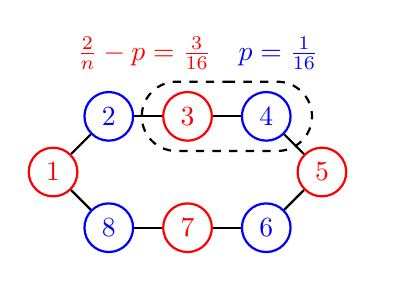
\begin{tikzpicture}[baseline=(current bounding box.north),-,auto,node distance=1cm,
                    thick,main node/.style={circle,draw,font=\sffamily\bfseries}]

  \node[main node,color=red] (1) {$1$};
  \node[main node,color=blue] (2) [above right of=1] {$2$};
  \node[main node,color=red] (3) [right of=2] {$3$};
  \node[main node,color=blue] (4) [right of=3] {$4$};
  \node[main node,color=red] (5) [below right of=4] {$5$};
  \node[main node,color=blue] (6) [below left of=5] {$6$};
  \node[main node,color=red] (7) [left of=6] {$7$};
  \node[main node,color=blue] (8) [left of=7] {$8$};
  

  \path[every node/.style={font=\sffamily}]
  (1) edge (2)
  (2) edge (3)
  (3) edge (4)
  (4) edge (5)
  (5) edge (6)
  (6) edge (7)
  (7) edge (8)
  (8) edge (1);
  
  \node (Box1) [draw,dashed,rounded rectangle,fit=(3) (4)] {};
  
  \node [shift={(-0.4cm,0.8cm)},text width=2cm,color=red] at (3) {$\frac{2}{n}-p=\frac{3}{16}$};
  \node [shift={(0.4cm,0.8cm)},text width=1.5cm,color=blue] at (4) {$p=\frac{1}{16}$};
   
\end{tikzpicture}
\end{center}
\caption{ $C_{8}$ with the \textcolor{blue}{blue nodes being ``even'' nodes} started at with probability $\frac{1}{16}$ and the \textcolor{red}{red nodes being ``odd'' nodes} started at with probability $\frac{3}{16}$.}
\end{examplefigure}

\begin{lemma}
When $n$ and $m$ are both even, following the Alternating Random Hamiltonian Patrol, if feasible, gives the same lower bound as the random Hamiltonian patrol, i.e $V \geq \frac{m}{n}$.
\end{lemma}

Proof: \ref{Alternating Random Hamiltonian proof}

If $m$ is odd, say $m=2m'+1$ then in the above we get two possibilities for each node depending on the interval choice either $p+\frac{m-1}{n}$ or $\frac{m+1}{n}-p$. So choosing anything other than $p=\frac{1}{n}$ (which is the Random Hamiltonian Patrol strategy) gives a worse result for the patroller.

While not getting a better lower bound, the ARHP does give some control on how to perform optimally in a Hamiltonian graph. The idea of distributing the probability $\frac{2}{n}$ between two types of nodes can be extended to the idea of distributing the probability $\frac{k}{n}$ between $k$ types of nodes.

As an extension to the Alternating Random Hamiltonian Patrol(ARHP) is the Block Random Hamiltonian Patrol(BRHP).

\begin{definition}[Block Random Hamiltonian Patrol(BRHP)]
A $k$ type \textit{Block Random Hamiltonian Patrol} (\textit{BRHP}) is a mixed strategy following the Hamiltonian Patrol but with a probability $p_{i}$ of starting at a ``type $i$'' node for $i=1,..,k$ , where $\sum\limits_{i=1}^{k} p_{i}=\frac{k}{n}$.
\end{definition}

\begin{lemma}
When $n$ and $m$ are both multiples of $k$, then following the $k$ type Block Random Hamiltonian Patrol, if feasible, gives the same lower bound as the random Hamiltonian patrol, i.e $V \geq \frac{m}{n}$
\end{lemma}

\begin{proof}
During any attack interval $I$ , which is of length $m=km'$, then $W(I)$ contains $m'$ ``type $i$'' nodes for $i=1,...,k$. Therefore by following the $k$ type BRHP, $\bm{\pi}_{BRHP}$, with probability $p_{i}$ at ``type $i$'' for $i=1,...,k$. Then

\begin{align*}
&P(\bm{\pi}_{BRHP},[i,I]) \geq \underbrace{\overbrace{p_{1}}^{\text{type } 1}+...+
\overbrace{p_{k}}^{\text{type } k}+p_{1}+...+p_{n}+...+...+p_{1}+...+p_{k}=2m'}_{\text{ m=km'elements}}= \\
&m' p_{1}+...+m'p_{k}=m' \frac{k}{n}=\frac{m}{n} \quad \forall i \in N \quad \forall I \subseteq \mathcal{T}
\end{align*}
Hence as it holds for all pure attacks
$$P(\bm{\pi}_{BRHP},\pmb{\phi}) \geq \frac{m}{n} \quad \forall \bm{\phi} \in \Phi$$
Hence $V \geq \frac{m}{n}$ .
\end{proof}

\begin{note}
In the one-off game, the BRHP strategy is always feasible. However in the periodic game, the BRHP strategy is only feasible if $T=k'n$ for some $k' \in \mathbb{N}$.
\end{note}

\section{Elongated star graph}
\subsection{Introduction}

The line and star graphs provided a good starting point for attempting to solving the problem with a general tree. If a more general version of the star graph can be solved, it may provide better bounds on a general tree and may in fact provide an exact solution (under certain conditions). 

The idea is to extend the star graph to a more general graph which is a mix between the line and the star, by extending the length of the branches (at first just one branch). This may better model a tightly packed region to search and another that is far away, consider the example of a small town and larger city connected by a road. 

\begin{definition}[Elongated Star Graph]
The \textit{Elongated Star Graph}, $S_{n}^k$ is made from $S_{n}$, by performing subdivision on one of the edges repeatedly $k$ times, so that one of the external nodes is now $k+1$ away from the centre.
\end{definition}

The labelling will be done as in Example Figure \ref{myfigure: Example of elongated labeling} and we will from now assume that $n \geq 3$, as otherwise we are just dealing with the line.


\begin{myfigure}
\begin{center}
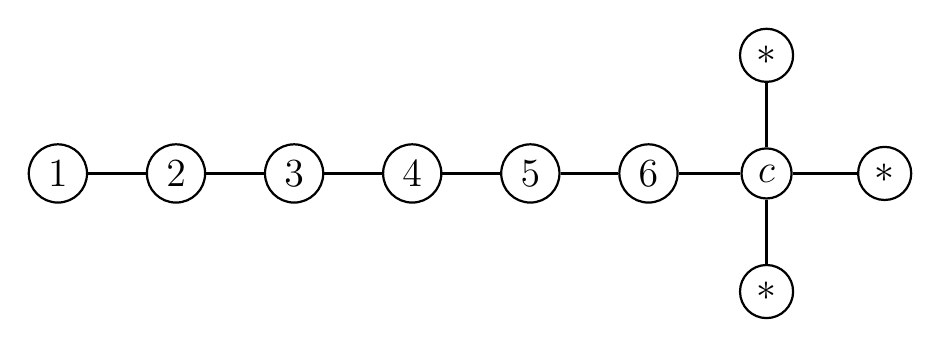
\begin{tikzpicture}[-,auto,node distance=1.5cm,
                    thick,main node/.style={circle,draw,font=\sffamily\Large\bfseries}]

  \node[main node] (1) {$1$};
  \node[main node] (2) [right of=1] {$2$};
  \node[main node] (3) [right of=2] {$3$};
  \node[main node] (4) [right of=3] {$4$};
  \node[main node] (5) [right of=4] {$5$};
  \node[main node] (6) [right of=5]  {$6$};
  \node[main node] (7) [right of=6]  {$c$};
  \node[main node] (8) [right of=7]  {$*$};
  \node[main node] (9) [above of=7]  {$*$};
  \node[main node] (10) [below of=7]  {$*$};
  

  \path[every node/.style={font=\sffamily}]
    (1) edge  (2)
    (2) edge (3)
    (3) edge (4)
    (4) edge (5)
    (5) edge (6)
    (6) edge (7)
    (7) edge (8)
     edge (9)
     edge (10);
\end{tikzpicture}
\end{center}
\caption{Labeling on the graph $S_{4}^5$.}
\label{myfigure: Example of elongated labeling}
\end{myfigure}

\subsection{Basic Analysis}
To start our analysis of this graph, we can look at an expanded graph which can simplify down to our extended star graph. Consider the cyclic graph $C_{(2k+1)+(2n-1)}=C_{2(n+k)}$, we can simplify this graph by node identifying. The identifying map is one such that we identify nodes $i$ to $2k+2-i$ for $i=1,..,k$ and identify nodes $2k+2,2k+4,..,2k+2n$.


\begin{myfigure}
\begin{center}
\resizebox{\textwidth}{!}{
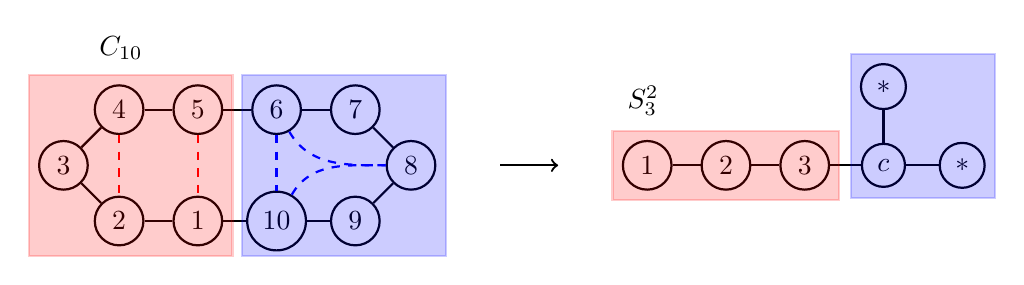
\begin{tikzpicture}[baseline=(current bounding box.north),-,auto,node distance=1cm,
                    thick,main node/.style={circle,draw,font=\sffamily\bfseries}]

  \node[main node] (1) {$3$};
  \node[main node] (2) [above right of=1] {$4$};
  \node[main node] (3) [right of=2] {$5$};
  \node[main node] (4) [right of=3] {$6$};
  \node[main node] (5) [right of=4] {$7$};
  \node[main node] (6) [below right of=5] {$8$};
  \node[main node] (7) [below right of=1] {$2$};
  \node[main node] (8) [right of=7] {$1$};
  \node[main node] (9) [right of=8] {$10$};
  \node[main node] (10) [right of=9] {$9$};
  
  \node (P1) [right of=6] {};
  \node (P2) [right of=P1] {};
  
  \node[main node] (a) [right of=P2] {$1$};
  \node[main node] (b) [right of=a] {$2$};
  \node[main node] (c) [right of=b] {$3$};
  \node[main node] (d) [right of=c] {$c$};
  \node[main node] (e) [right of=d] {$*$};
  \node[main node] (f) [above of=d] {$*$};
  
  \draw[->] (P1) edge (P2);
  

  \path[every node/.style={font=\sffamily}]
    (1) edge  (2)
    edge (7)
    (2) edge (3)
    (3) edge (4)
    (4) edge (5)
    (5) edge (6)
    (6) edge (10)
    (7) edge (8)
    (8) edge (9)
    (9) edge (10)
    (a) edge (b)
    (b) edge (c)
    (c) edge (d)
    (d) edge (e)
    edge (f);
    
     \path[dashed,red,every node/.style={font=\sffamily}]
    (2) edge  (7)
    (3) edge (8);
    
    \path[dashed,blue,every node/.style={font=\sffamily}]
    (4) edge  (9);
    
    \path[dashed,blue,out=-60,in=180,every node/.style={font=\sffamily}]
    (4) edge (6);
    
    \path[dashed,blue,out=60,in=180,every node/.style={font=\sffamily}]
    (9) edge (6);
  
  \node (Box1) [draw,thick,fit=(1) (2) (3) (7) (8),fill,red,opacity=0.2] {};
  \node (Box2) [draw,thick,fit=(4) (5) (6)  (10),fill,blue,opacity=0.2] {};
  
  \node (Box3) [draw,thick,fit=(a) (b) (c),fill,red,opacity=0.2] {}; 
  \node (Box4) [draw,thick,fit=(d) (e) (f),fill,blue,opacity=0.2] {};   
  
\node [left=0.5cm,above=0.5cm,text width=0.5cm] at (2) {$C_{10}$};
\node [left=0.5cm,above=0.5cm,text width=0.5cm] at (a) {$S_{3}^{2}$};   
\end{tikzpicture}
}
\end{center}
\caption{$C_{10}$ can be simplified to $S_{3}^{2}$ by node identifying.}
\end{myfigure}


\begin{definition}[Random Oscillation]
The \textit{Oscillation} on $S_{n}^{k}$ is any embedded Hamiltonian Patrol on $C_{2(n+k)}$ under the simplification above.
The \textit{Random Oscillation} on $S_{n}^{k}$ is the embedded Random Hamiltonian Patrol on $C_{2(n+k)}$ under the simplification above.
\end{definition}

\begin{lemma}
For $m < 2(n+k)$ following the Random Oscillation,
$$V(S_{n}^{k}) \geq V(C_{2(n+k)})=\frac{m}{2(n+k)}$$
and if $m \geq 2(n+k)$ then $V(S_{n}^{k})=1$, achieved by any Oscillation.
\end{lemma}

Hence we have the solution in $m \geq 2(n+k)$ , so we can now restrict ourselves to $m < 2(n+k)$.


\begin{myfigure}
\begin{center}
\resizebox{.6\textwidth}{!}{
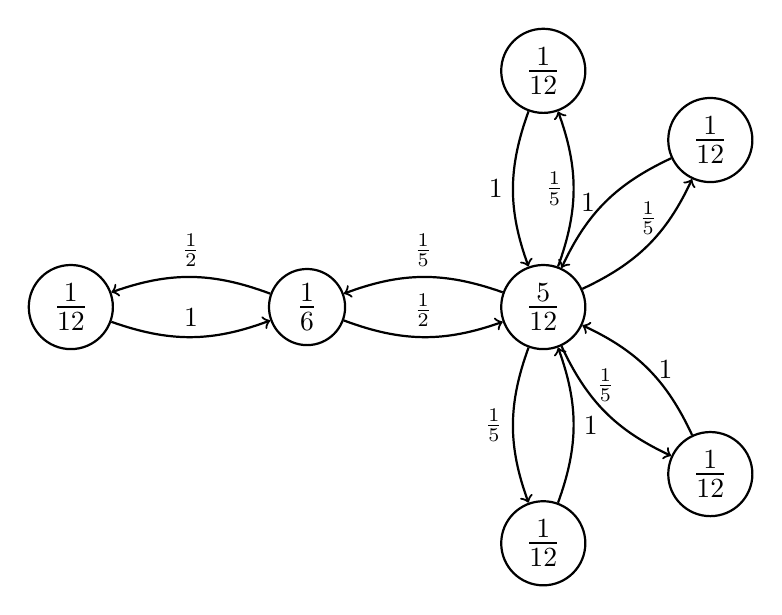
\begin{tikzpicture}[-,auto,node distance=3cm,
                    thick,main node/.style={circle,draw,font=\sffamily\Large\bfseries}]

  \node[main node] (1) {$\frac{5}{12}$};
  \node[main node] (2) [below of=1] {$\frac{1}{12}$};
  \node[main node] (3) [below right of=1] {$\frac{1}{12}$};
  \node[main node] (4) [above right of=1]  {$\frac{1}{12}$};
  \node[main node] (5) [above of=1]  {$\frac{1}{12}$};
  \node[main node] (6) [left of=1]  {$\frac{1}{6}$};
  \node[main node] (7) [left of=6] {$\frac{1}{12}$};

  \path[->,bend right,out=-20,in=200,every node/.style={font=\sffamily}]
    (1) edge node[,midway,left] {$\frac{1}{5}$} (2)
    edge node[midway,above] {$\frac{1}{5}$} (3) 
    edge node[midway,above] {$\frac{1}{5}$} (4)
    edge node[midway,left] {$\frac{1}{5}$} (5) 
    edge node[midway,above] {$\frac{1}{5}$} (6) 
    (2) edge node[midway,right] {$1$} (1) 
    (3) edge node[midway,right] {$1$} (1) 
    (4) edge node[midway,left] {$1$} (1) 
    (5) edge node[midway,left] {$1$} (1) 
    (6) edge node[midway] {$\frac{1}{2}$} (1) 
    edge node[midway,above] {$\frac{1}{2}$} (7) 
    (7) edge node[midway] {$1$} (6);
    
%\node [right=4cm , text width=5cm,font=\footnotesize] at (1)    
%{
%The Starting Probabilities are shown inside the nodes and the initial movement probabilities are shown on the edges.
%};    
\end{tikzpicture}
}
\end{center}
\caption{Starting points and initial movements of the Random Oscillation on $S_{5}^{1}$.}
\end{myfigure}


Next we look at getting an attacker bound. In $S_{n}$, the use of the equal weighting at each external nodes is similar to the diametric attack proposed in \cite{Alpern2011} but now picks the set of all points mutually at diameter. A natural analogue of this is to use some weighting depending on the length they are away from the centre.

\begin{definition}[Weighted External Attack]
The \textit{Weighted External Attack} attacks at node $1$ with probability $\frac{k+1}{n+k} $ and at each $*$ node with probability $\frac{1}{n+k}$ for a random attack interval $I$.
\end{definition}

The idea of the weighted external attack is that we can form the upper bound $V \leq \frac{m}{2(n+k)}$. However, unlike first thought, it does not seem to give the upper bound as we wished, the problem is clear that for a small time horizon there is an issue of being able to achieve a better patrolling strategy (as seen in example \ref{example:Weightedexternal}).



\subsection{Solution for $m \geq 2(k+1)$}

We will match the Oscillation bound of $\frac{m}{2(n+k)}$, by developing a further extended version of time-limited attack.

\begin{definition}[Time-delayed attack]
Let the \textit{time-delayed attack}, be the attack that attacks at the extended node labeled $1$ with probability $\frac{k+1}{n+k}$ and a particular normal node labeled $*$ with probability $\frac{1}{n+k}$.

If node $1$ is chosen have the attack choose probability intervals with equal probability at the times $I,I+1,...,I+2k+1$ for some $I$ (i.e starting attacks at $\tau, \tau+1,...,\tau+2k+1$). If a $*$ node is chosen start the attacks at the times $I+k,I+k+1$ with equal probability.
\end{definition}

\begin{myfigure}
\begin{center}
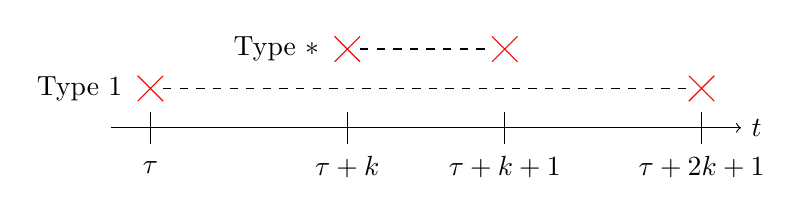
\begin{tikzpicture}
 %Drawing Bottom Axis
 \draw[->] (-4,0) -- (4,0);
 \node (timelabel) [shift={(0.2,0)}] at (4,0) {$t$};
 \draw (-3.5,0.2) -- (-3.5,-0.2);
 \draw (3.5,0.2) -- (3.5,-0.2);
 
 %Drawing Cross and lines 
 \node (labelc1) at (-3.5,-0.5) {$\tau$};
 \node (labelc2) at (3.5,-0.5) {$\tau+2k+1$};
 
 \node[cross=5pt,red] (c1) at (-3.5,0.5) {};
 \node[cross=5pt,red] (c2) at (3.5,0.5) {};
 \draw[dashed] (c1) -- (c2);
 \node (linelabel1) at (-4.4,0.5) {Type $1$};
 
 
 \draw (-1,0.2) -- (-1,-0.2);
 \draw (1,0.2) -- (1,-0.2);
 
  \node (labelc3) at (-1,-0.5) {$\tau+k$};
 \node (labelc4) at (1,-0.5) {$\tau+k+1$};
 
 \node[cross=5pt,red] (c3) at (-1,1) {};
 \node[cross=5pt,red] (c4) at (1,1) {};
 \draw[dashed] (c3) -- (c4);
 \node (linelabel1) at (-1.9,1) {Type $*$}; 

\end{tikzpicture}
\end{center}
\end{myfigure}

Note. The time-delayed attack uses the weighted suggested previously but delays the normal star ends starting times (and has them only occur for a shorter period of time)


\begin{lemma}
When $T \geq m+2k$, the analogous `diametric' bound $V \leq \max \{ \frac{k+1}{n+k} , \frac{m}{2(n+k)}   \}$ is valid
\end{lemma}

Proof: \ref{T-delayed attack proof}

With this result we have the solution in our range

\begin{lemma}[Solution in $m \geq 2(k+1)$]
By the attacker using the stage-delayed attack and the patroller using a random oscillation patrol, we achieve the value, when $2(k+1) \leq m \leq 2(n+k)$
$$V=\frac{m}{2(n+k)}$$
\end{lemma}

Hence we have a solution for 2 regions $m > 2(n+k)$ and $2(k+1) \leq m \leq 2(n+k)$

\begin{myfigure}
\resizebox{0.95\linewidth}{!}{
% Created by tikzDevice version 0.10.1 on 2017-11-10 10:35:56
% !TEX encoding = UTF-8 Unicode
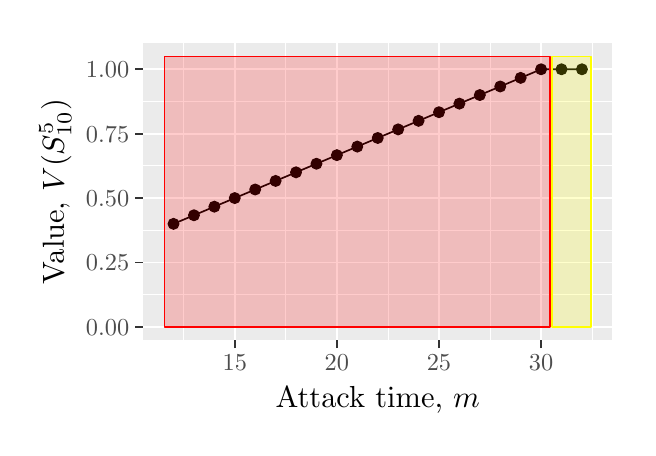
\begin{tikzpicture}[x=1pt,y=1pt]
\definecolor{fillColor}{RGB}{255,255,255}
\path[use as bounding box,fill=fillColor,fill opacity=0.00] (0,0) rectangle (216.81,144.54);
\begin{scope}
\path[clip] (  0.00,  0.00) rectangle (216.81,144.54);
\definecolor{drawColor}{RGB}{255,255,255}
\definecolor{fillColor}{RGB}{255,255,255}

\path[draw=drawColor,line width= 0.6pt,line join=round,line cap=round,fill=fillColor] (  0.00,  0.00) rectangle (216.81,144.54);
\end{scope}
\begin{scope}
\path[clip] ( 41.67, 31.53) rectangle (211.31,139.04);
\definecolor{fillColor}{gray}{0.92}

\path[fill=fillColor] ( 41.67, 31.53) rectangle (211.31,139.04);
\definecolor{drawColor}{RGB}{255,255,255}

\path[draw=drawColor,line width= 0.3pt,line join=round] ( 41.67, 48.05) --
	(211.31, 48.05);

\path[draw=drawColor,line width= 0.3pt,line join=round] ( 41.67, 71.32) --
	(211.31, 71.32);

\path[draw=drawColor,line width= 0.3pt,line join=round] ( 41.67, 94.59) --
	(211.31, 94.59);

\path[draw=drawColor,line width= 0.3pt,line join=round] ( 41.67,117.86) --
	(211.31,117.86);

\path[draw=drawColor,line width= 0.3pt,line join=round] ( 56.39, 31.53) --
	( 56.39,139.04);

\path[draw=drawColor,line width= 0.3pt,line join=round] ( 93.28, 31.53) --
	( 93.28,139.04);

\path[draw=drawColor,line width= 0.3pt,line join=round] (130.18, 31.53) --
	(130.18,139.04);

\path[draw=drawColor,line width= 0.3pt,line join=round] (167.07, 31.53) --
	(167.07,139.04);

\path[draw=drawColor,line width= 0.3pt,line join=round] (203.97, 31.53) --
	(203.97,139.04);

\path[draw=drawColor,line width= 0.6pt,line join=round] ( 41.67, 36.42) --
	(211.31, 36.42);

\path[draw=drawColor,line width= 0.6pt,line join=round] ( 41.67, 59.69) --
	(211.31, 59.69);

\path[draw=drawColor,line width= 0.6pt,line join=round] ( 41.67, 82.96) --
	(211.31, 82.96);

\path[draw=drawColor,line width= 0.6pt,line join=round] ( 41.67,106.23) --
	(211.31,106.23);

\path[draw=drawColor,line width= 0.6pt,line join=round] ( 41.67,129.50) --
	(211.31,129.50);

\path[draw=drawColor,line width= 0.6pt,line join=round] ( 74.83, 31.53) --
	( 74.83,139.04);

\path[draw=drawColor,line width= 0.6pt,line join=round] (111.73, 31.53) --
	(111.73,139.04);

\path[draw=drawColor,line width= 0.6pt,line join=round] (148.63, 31.53) --
	(148.63,139.04);

\path[draw=drawColor,line width= 0.6pt,line join=round] (185.52, 31.53) --
	(185.52,139.04);
\definecolor{drawColor}{RGB}{0,0,0}
\definecolor{fillColor}{RGB}{0,0,0}

\path[draw=drawColor,line width= 0.4pt,line join=round,line cap=round,fill=fillColor] (192.90,129.50) circle (  1.96);

\path[draw=drawColor,line width= 0.4pt,line join=round,line cap=round,fill=fillColor] (200.28,129.50) circle (  1.96);

\path[draw=drawColor,line width= 0.4pt,line join=round,line cap=round,fill=fillColor] ( 52.70, 73.65) circle (  1.96);

\path[draw=drawColor,line width= 0.4pt,line join=round,line cap=round,fill=fillColor] ( 60.08, 76.75) circle (  1.96);

\path[draw=drawColor,line width= 0.4pt,line join=round,line cap=round,fill=fillColor] ( 67.46, 79.86) circle (  1.96);

\path[draw=drawColor,line width= 0.4pt,line join=round,line cap=round,fill=fillColor] ( 74.83, 82.96) circle (  1.96);

\path[draw=drawColor,line width= 0.4pt,line join=round,line cap=round,fill=fillColor] ( 82.21, 86.06) circle (  1.96);

\path[draw=drawColor,line width= 0.4pt,line join=round,line cap=round,fill=fillColor] ( 89.59, 89.16) circle (  1.96);

\path[draw=drawColor,line width= 0.4pt,line join=round,line cap=round,fill=fillColor] ( 96.97, 92.27) circle (  1.96);

\path[draw=drawColor,line width= 0.4pt,line join=round,line cap=round,fill=fillColor] (104.35, 95.37) circle (  1.96);

\path[draw=drawColor,line width= 0.4pt,line join=round,line cap=round,fill=fillColor] (111.73, 98.47) circle (  1.96);

\path[draw=drawColor,line width= 0.4pt,line join=round,line cap=round,fill=fillColor] (119.11,101.57) circle (  1.96);

\path[draw=drawColor,line width= 0.4pt,line join=round,line cap=round,fill=fillColor] (126.49,104.68) circle (  1.96);

\path[draw=drawColor,line width= 0.4pt,line join=round,line cap=round,fill=fillColor] (133.87,107.78) circle (  1.96);

\path[draw=drawColor,line width= 0.4pt,line join=round,line cap=round,fill=fillColor] (141.25,110.88) circle (  1.96);

\path[draw=drawColor,line width= 0.4pt,line join=round,line cap=round,fill=fillColor] (148.63,113.99) circle (  1.96);

\path[draw=drawColor,line width= 0.4pt,line join=round,line cap=round,fill=fillColor] (156.00,117.09) circle (  1.96);

\path[draw=drawColor,line width= 0.4pt,line join=round,line cap=round,fill=fillColor] (163.38,120.19) circle (  1.96);

\path[draw=drawColor,line width= 0.4pt,line join=round,line cap=round,fill=fillColor] (170.76,123.29) circle (  1.96);

\path[draw=drawColor,line width= 0.4pt,line join=round,line cap=round,fill=fillColor] (178.14,126.40) circle (  1.96);

\path[draw=drawColor,line width= 0.4pt,line join=round,line cap=round,fill=fillColor] (185.52,129.50) circle (  1.96);

\path[draw=drawColor,line width= 0.6pt,line join=round] ( 52.70, 73.65) --
	( 60.08, 76.75) --
	( 67.46, 79.86) --
	( 74.83, 82.96) --
	( 82.21, 86.06) --
	( 89.59, 89.16) --
	( 96.97, 92.27) --
	(104.35, 95.37) --
	(111.73, 98.47) --
	(119.11,101.57) --
	(126.49,104.68) --
	(133.87,107.78) --
	(141.25,110.88) --
	(148.63,113.99) --
	(156.00,117.09) --
	(163.38,120.19) --
	(170.76,123.29) --
	(178.14,126.40) --
	(185.52,129.50) --
	(192.90,129.50) --
	(200.28,129.50);
\definecolor{drawColor}{RGB}{255,255,0}
\definecolor{fillColor}{RGB}{255,255,0}

\path[draw=drawColor,line width= 0.6pt,line join=round,fill=fillColor,fill opacity=0.20] (189.58, 36.42) rectangle (203.60,134.15);
\definecolor{drawColor}{RGB}{255,0,0}
\definecolor{fillColor}{RGB}{255,0,0}

\path[draw=drawColor,line width= 0.6pt,line join=round,fill=fillColor,fill opacity=0.20] ( 49.38, 36.42) rectangle (188.84,134.15);
\end{scope}
\begin{scope}
\path[clip] (  0.00,  0.00) rectangle (216.81,144.54);
\definecolor{drawColor}{gray}{0.30}

\node[text=drawColor,anchor=base east,inner sep=0pt, outer sep=0pt, scale=  0.88] at ( 36.72, 33.39) {0.00};

\node[text=drawColor,anchor=base east,inner sep=0pt, outer sep=0pt, scale=  0.88] at ( 36.72, 56.66) {0.25};

\node[text=drawColor,anchor=base east,inner sep=0pt, outer sep=0pt, scale=  0.88] at ( 36.72, 79.93) {0.50};

\node[text=drawColor,anchor=base east,inner sep=0pt, outer sep=0pt, scale=  0.88] at ( 36.72,103.20) {0.75};

\node[text=drawColor,anchor=base east,inner sep=0pt, outer sep=0pt, scale=  0.88] at ( 36.72,126.47) {1.00};
\end{scope}
\begin{scope}
\path[clip] (  0.00,  0.00) rectangle (216.81,144.54);
\definecolor{drawColor}{gray}{0.20}

\path[draw=drawColor,line width= 0.6pt,line join=round] ( 38.92, 36.42) --
	( 41.67, 36.42);

\path[draw=drawColor,line width= 0.6pt,line join=round] ( 38.92, 59.69) --
	( 41.67, 59.69);

\path[draw=drawColor,line width= 0.6pt,line join=round] ( 38.92, 82.96) --
	( 41.67, 82.96);

\path[draw=drawColor,line width= 0.6pt,line join=round] ( 38.92,106.23) --
	( 41.67,106.23);

\path[draw=drawColor,line width= 0.6pt,line join=round] ( 38.92,129.50) --
	( 41.67,129.50);
\end{scope}
\begin{scope}
\path[clip] (  0.00,  0.00) rectangle (216.81,144.54);
\definecolor{drawColor}{gray}{0.20}

\path[draw=drawColor,line width= 0.6pt,line join=round] ( 74.83, 28.78) --
	( 74.83, 31.53);

\path[draw=drawColor,line width= 0.6pt,line join=round] (111.73, 28.78) --
	(111.73, 31.53);

\path[draw=drawColor,line width= 0.6pt,line join=round] (148.63, 28.78) --
	(148.63, 31.53);

\path[draw=drawColor,line width= 0.6pt,line join=round] (185.52, 28.78) --
	(185.52, 31.53);
\end{scope}
\begin{scope}
\path[clip] (  0.00,  0.00) rectangle (216.81,144.54);
\definecolor{drawColor}{gray}{0.30}

\node[text=drawColor,anchor=base,inner sep=0pt, outer sep=0pt, scale=  0.88] at ( 74.83, 20.52) {15};

\node[text=drawColor,anchor=base,inner sep=0pt, outer sep=0pt, scale=  0.88] at (111.73, 20.52) {20};

\node[text=drawColor,anchor=base,inner sep=0pt, outer sep=0pt, scale=  0.88] at (148.63, 20.52) {25};

\node[text=drawColor,anchor=base,inner sep=0pt, outer sep=0pt, scale=  0.88] at (185.52, 20.52) {30};
\end{scope}
\begin{scope}
\path[clip] (  0.00,  0.00) rectangle (216.81,144.54);
\definecolor{drawColor}{RGB}{0,0,0}

\node[text=drawColor,anchor=base,inner sep=0pt, outer sep=0pt, scale=  1.10] at (126.49,  7.44) {Attack time, $m$};
\end{scope}
\begin{scope}
\path[clip] (  0.00,  0.00) rectangle (216.81,144.54);
\definecolor{drawColor}{RGB}{0,0,0}

\node[text=drawColor,rotate= 90.00,anchor=base,inner sep=0pt, outer sep=0pt, scale=  1.10] at ( 13.08, 85.29) {Value, $V(S_{ 10 }^{ 5 })$};
\end{scope}
\end{tikzpicture}
}
\caption{Value of the Star Graph, $S_{10}^{5}$}
\end{myfigure}

\subsection{Solutions below Hamiltonian boundary}
We now seek solutions below the Hamiltonian bound of value $ \frac{m}{2(n+k)}$. In this region like in the line graph regions below oscillation boundary, we expect the patroller can do better in some fashion.

Guess: Some concave type region will exist below.

\subsection{Improving the Hamiltonian bound}
We could suggest a similar improvement to that done on the line, that is to improve the probability of intercepting an attack when following the random oscillation

\textbf{Probability of interception}

If the patroller is performing a Random Oscillation, then for a pure attack at node $i$ the probability of capture is given by (derivation in appednix \ref{appednixsection: Reason for probability of interception}),
\begin{equation}
\label{eq:Prob of Interception}
w(i)= \left\{\begin{array}{l}
 \frac{\min(m+2(i-1),2m)}{2(n+k)} \text{  , for } i \leq \frac{n+k}{2} +1, \\
 \frac{\min(m+2(n+k+1-i),2m)}{2(n+k)} \text{  , for } i > \frac{n+k}{2} +1, \\
 \frac{\min(m+2(n-1),nm)}{2(n+k)} \text{  , for } i=c, \\
 \frac{m}{2(n+k)} \text{  , for } i=*. 
\end{array} \right.
\end{equation}
We will call $w(i)$ the probability of \textit{interception} at node $i$.


\begin{examplefigure}
\begin{center}
% Created by tikzDevice version 0.12 on 2019-02-23 16:13:44
% !TEX encoding = UTF-8 Unicode
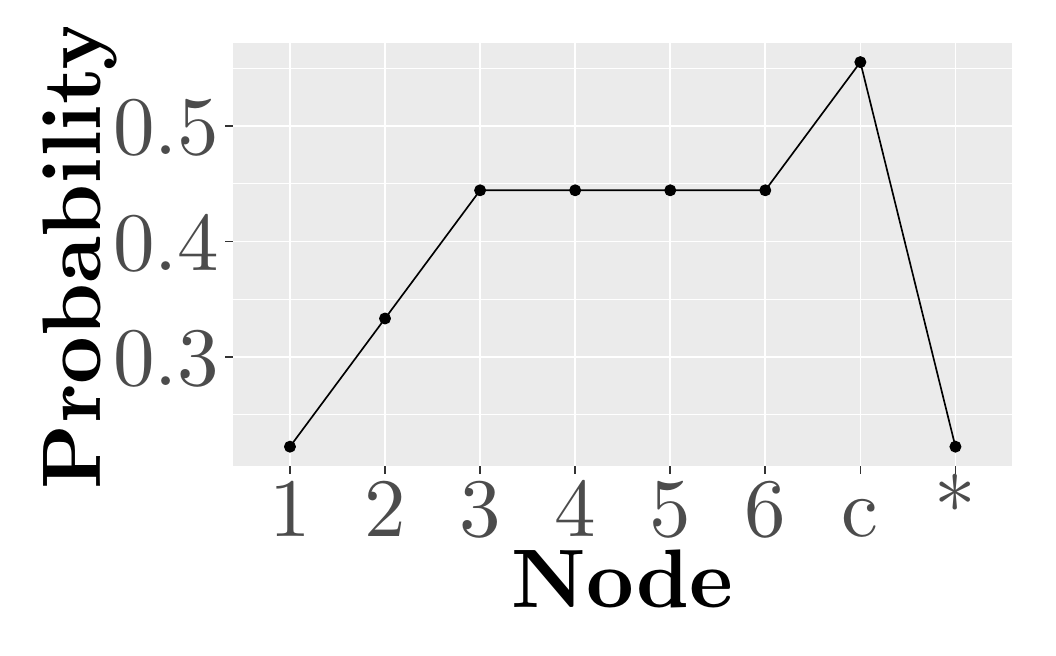
\begin{tikzpicture}[x=1pt,y=1pt]
\definecolor{fillColor}{RGB}{255,255,255}
\path[use as bounding box,fill=fillColor,fill opacity=0.00] (0,0) rectangle (361.35,216.81);
\begin{scope}
\path[clip] (  0.00,  0.00) rectangle (361.35,216.81);
\definecolor{drawColor}{RGB}{255,255,255}
\definecolor{fillColor}{RGB}{255,255,255}

\path[draw=drawColor,line width= 0.6pt,line join=round,line cap=round,fill=fillColor] (  0.00,  0.00) rectangle (361.35,216.81);
\end{scope}
\begin{scope}
\path[clip] ( 74.17, 58.45) rectangle (355.85,211.31);
\definecolor{fillColor}{gray}{0.92}

\path[fill=fillColor] ( 74.17, 58.45) rectangle (355.85,211.31);
\definecolor{drawColor}{RGB}{255,255,255}

\path[draw=drawColor,line width= 0.3pt,line join=round] ( 74.17, 76.98) --
	(355.85, 76.98);

\path[draw=drawColor,line width= 0.3pt,line join=round] ( 74.17,118.67) --
	(355.85,118.67);

\path[draw=drawColor,line width= 0.3pt,line join=round] ( 74.17,160.36) --
	(355.85,160.36);

\path[draw=drawColor,line width= 0.3pt,line join=round] ( 74.17,202.05) --
	(355.85,202.05);

\path[draw=drawColor,line width= 0.6pt,line join=round] ( 74.17, 97.83) --
	(355.85, 97.83);

\path[draw=drawColor,line width= 0.6pt,line join=round] ( 74.17,139.51) --
	(355.85,139.51);

\path[draw=drawColor,line width= 0.6pt,line join=round] ( 74.17,181.20) --
	(355.85,181.20);

\path[draw=drawColor,line width= 0.6pt,line join=round] ( 94.78, 58.45) --
	( 94.78,211.31);

\path[draw=drawColor,line width= 0.6pt,line join=round] (129.13, 58.45) --
	(129.13,211.31);

\path[draw=drawColor,line width= 0.6pt,line join=round] (163.48, 58.45) --
	(163.48,211.31);

\path[draw=drawColor,line width= 0.6pt,line join=round] (197.84, 58.45) --
	(197.84,211.31);

\path[draw=drawColor,line width= 0.6pt,line join=round] (232.19, 58.45) --
	(232.19,211.31);

\path[draw=drawColor,line width= 0.6pt,line join=round] (266.54, 58.45) --
	(266.54,211.31);

\path[draw=drawColor,line width= 0.6pt,line join=round] (300.89, 58.45) --
	(300.89,211.31);

\path[draw=drawColor,line width= 0.6pt,line join=round] (335.24, 58.45) --
	(335.24,211.31);
\definecolor{drawColor}{RGB}{0,0,0}
\definecolor{fillColor}{RGB}{0,0,0}

\path[draw=drawColor,line width= 0.4pt,line join=round,line cap=round,fill=fillColor] ( 94.78, 65.40) circle (  1.96);

\path[draw=drawColor,line width= 0.4pt,line join=round,line cap=round,fill=fillColor] (129.13,111.72) circle (  1.96);

\path[draw=drawColor,line width= 0.4pt,line join=round,line cap=round,fill=fillColor] (163.48,158.04) circle (  1.96);

\path[draw=drawColor,line width= 0.4pt,line join=round,line cap=round,fill=fillColor] (197.84,158.04) circle (  1.96);

\path[draw=drawColor,line width= 0.4pt,line join=round,line cap=round,fill=fillColor] (232.19,158.04) circle (  1.96);

\path[draw=drawColor,line width= 0.4pt,line join=round,line cap=round,fill=fillColor] (266.54,158.04) circle (  1.96);

\path[draw=drawColor,line width= 0.4pt,line join=round,line cap=round,fill=fillColor] (300.89,204.36) circle (  1.96);

\path[draw=drawColor,line width= 0.4pt,line join=round,line cap=round,fill=fillColor] (335.24, 65.40) circle (  1.96);

\path[draw=drawColor,line width= 0.6pt,line join=round] ( 94.78, 65.40) --
	(129.13,111.72) --
	(163.48,158.04) --
	(197.84,158.04) --
	(232.19,158.04) --
	(266.54,158.04) --
	(300.89,204.36) --
	(335.24, 65.40);
\end{scope}
\begin{scope}
\path[clip] (  0.00,  0.00) rectangle (361.35,216.81);
\definecolor{drawColor}{gray}{0.30}

\node[text=drawColor,anchor=base east,inner sep=0pt, outer sep=0pt, scale=  3.00] at ( 69.22, 87.49) {0.3};

\node[text=drawColor,anchor=base east,inner sep=0pt, outer sep=0pt, scale=  3.00] at ( 69.22,129.18) {0.4};

\node[text=drawColor,anchor=base east,inner sep=0pt, outer sep=0pt, scale=  3.00] at ( 69.22,170.87) {0.5};
\end{scope}
\begin{scope}
\path[clip] (  0.00,  0.00) rectangle (361.35,216.81);
\definecolor{drawColor}{gray}{0.20}

\path[draw=drawColor,line width= 0.6pt,line join=round] ( 71.42, 97.83) --
	( 74.17, 97.83);

\path[draw=drawColor,line width= 0.6pt,line join=round] ( 71.42,139.51) --
	( 74.17,139.51);

\path[draw=drawColor,line width= 0.6pt,line join=round] ( 71.42,181.20) --
	( 74.17,181.20);
\end{scope}
\begin{scope}
\path[clip] (  0.00,  0.00) rectangle (361.35,216.81);
\definecolor{drawColor}{gray}{0.20}

\path[draw=drawColor,line width= 0.6pt,line join=round] ( 94.78, 55.70) --
	( 94.78, 58.45);

\path[draw=drawColor,line width= 0.6pt,line join=round] (129.13, 55.70) --
	(129.13, 58.45);

\path[draw=drawColor,line width= 0.6pt,line join=round] (163.48, 55.70) --
	(163.48, 58.45);

\path[draw=drawColor,line width= 0.6pt,line join=round] (197.84, 55.70) --
	(197.84, 58.45);

\path[draw=drawColor,line width= 0.6pt,line join=round] (232.19, 55.70) --
	(232.19, 58.45);

\path[draw=drawColor,line width= 0.6pt,line join=round] (266.54, 55.70) --
	(266.54, 58.45);

\path[draw=drawColor,line width= 0.6pt,line join=round] (300.89, 55.70) --
	(300.89, 58.45);

\path[draw=drawColor,line width= 0.6pt,line join=round] (335.24, 55.70) --
	(335.24, 58.45);
\end{scope}
\begin{scope}
\path[clip] (  0.00,  0.00) rectangle (361.35,216.81);
\definecolor{drawColor}{gray}{0.30}

\node[text=drawColor,anchor=base,inner sep=0pt, outer sep=0pt, scale=  3.00] at ( 94.78, 32.84) {1};

\node[text=drawColor,anchor=base,inner sep=0pt, outer sep=0pt, scale=  3.00] at (129.13, 32.84) {2};

\node[text=drawColor,anchor=base,inner sep=0pt, outer sep=0pt, scale=  3.00] at (163.48, 32.84) {3};

\node[text=drawColor,anchor=base,inner sep=0pt, outer sep=0pt, scale=  3.00] at (197.84, 32.84) {4};

\node[text=drawColor,anchor=base,inner sep=0pt, outer sep=0pt, scale=  3.00] at (232.19, 32.84) {5};

\node[text=drawColor,anchor=base,inner sep=0pt, outer sep=0pt, scale=  3.00] at (266.54, 32.84) {6};

\node[text=drawColor,anchor=base,inner sep=0pt, outer sep=0pt, scale=  3.00] at (300.89, 32.84) {c};

\node[text=drawColor,anchor=base,inner sep=0pt, outer sep=0pt, scale=  3.00] at (335.24, 32.84) {*};
\end{scope}
\begin{scope}
\path[clip] (  0.00,  0.00) rectangle (361.35,216.81);
\definecolor{drawColor}{RGB}{0,0,0}

\node[text=drawColor,anchor=base,inner sep=0pt, outer sep=0pt, scale=  3.00] at (215.01,  7.44) {\bfseries Node};
\end{scope}
\begin{scope}
\path[clip] (  0.00,  0.00) rectangle (361.35,216.81);
\definecolor{drawColor}{RGB}{0,0,0}

\node[text=drawColor,rotate= 90.00,anchor=base,inner sep=0pt, outer sep=0pt, scale=  3.00] at ( 26.20,134.88) {\bfseries Probability};
\end{scope}
\end{tikzpicture}

\end{center}
\caption{Interception probabilities of $S^5_{4}$ when $m=4$.}
\end{examplefigure}


\begin{definition}[End-ensuring cycle]
Define a cycle of length $m$ (if even) or $m-1$ (if odd) to be \textit{End-ensuring} if one of the points along the cycle is a leaf node. Define the \textit{Half-length} of such cycles to be $\hat{m}=\floor{\frac{m}{2}}$.
\end{definition}

As End-ensuring cycles return to all the nodes in the cycle every $m$ (if even) or $m-1$ (if odd) it means that any pure attack against a node in the End-ensuring cycle will be guaranteed to be caught by such a patrol.

In \cite{Papadaki2016} the authors improved nodes with poor interception probabilities by introducing two End-ensuring cycles. We shall do the same, though now more consideration needs to be taken on how to place these End-ensuring cycles. 

The minimum probability of interception, $w_{min} \equiv \min\limits_{i=1,..,k+1,c,*} w(i)$, gives the lower bound $V \geq w_{min}$. Hence improving this minimum will improve the lower bound. As it stands $w(1)=w(*)=w_{min}$, so improvement is required about $1$ and $*$.

First consider partitioning the node set, $N$, into $L=\left\{ i \, | \, i \leq \floor{\frac{m}{2}}+1 , i \leq k+1 \right\}$ , $M=\left\{ i \, | \, \floor{\frac{m}{2}}+2 \leq i \leq n+k-\floor{\frac{m}{2}} , i \leq k+1 \right\}$ , $R=\left\{ i \, | \, i \geq n+k+1-\floor{\frac{m}{2}} , i \leq k+1 \right\}$ , $S=\{ c,* \}$. Then $w_{min} \equiv w_{\min}^{N}=\min \{ w_{min}^{L},w_{min}^{M},w_{min}^{R},w_{min}^{S} \}$ , where $w_{min}^{X}=\min\limits_{i \in X} w(i)$.

Note. The set $R$ is empty if $\floor{\frac{m}{2}} \leq n-1$. The set $M$ is empty if $\floor{\frac{m}{2}} \geq k-1$ or $\floor{\frac{m}{2}} \geq n+k-2$.

Now from equation \ref{eq:Prob of Interception}
\begin{itemize}
\item $w_{min}^{L}=w(1)$, as for $i \in L$ we have that $w(i)$ is increasing in $i$.
\item $w_{min}^{M}=w(\floor{\frac{m}{2}}+2)=\frac{2m}{2(n+k)}$ , as for $i \in M $ we have that $w(i)=\frac{2m}{2(n+k)}$ $\forall i \in M$.
\item $w_{min}^{R}=w(k+1)$, as for $i \in R$ we have that $w(i)$ is decreasing in $i$.
\item $w_{min}^{S}=w(*)$, as $w(c) > w(*)$.
\end{itemize}

So as long as the improvement made on $L$ and $M$ is non-decreasing then only the nodes $1$ and $\floor{\frac{m}{2}}+2$ need be considered. Similarly if in $R$, the improvement is non-increasing then we only need to consider the node $k+1$.Finally if in $S$, the improvement improves node $c$ as good as $*$ then we only need to consider $*$. Therefore we shall only consider such improvement strategies.

Similarly let $C_{\min}^{X} (\bm{\pi}) = \min\limits_{i \in X} P(\bm{\pi},i)$, where $P(\bm{\pi},i)=\max\limits_{ I \subset \mathcal{T}} P(\bm{\pi},[i,I])$, be the probability of capture under $\bm{\pi}$ and $C_{\min} (\bm{\pi}) \equiv C_{\min}^{N} = \min \{ C_{\min}^{L},  C_{\min}^{M},  C_{\min}^{R},  C_{\min}^{S} \}$. Then we seek to select $\bm{\pi}$ to get $C_{\min} (\bm{\pi}) > W_{\min} \equiv C_{\min}(\bm{\pi}_{0})$ , where $\bm{\pi}_{0}$ is the Random Oscillation strategy.

We will use $P$ to be the probability the Random Oscillation is played and $Q=1-P$. Let $Q=Q_{L}+Q_{M}+Q_{R}+Q_{S}$, where $Q_{X}$ is the amount of probability used to improve the probability of intersection for the set $X$. We use $q_{X}$ to be probability that the minimum of the set is improved by, so $C_{\min}^{X}=PW_{\min}^{X}+q_{X}$.


\textbf{A Naive Improvement}
Let $\bm{\pi}=\alpha(Q_{L},Q_{S})$ denote the Naive Improvement Policy.
We will play the end-ensuring cycle, $\{1,...,\floor{\frac{m}{2}}+1,...,1\}$, with probability $Q_{L}$ (a non-decreasing improvement), giving $q_{L}=Q_{L}$. We will play,  with probability $Q_{S}$, an end-ensuring cycle for each $*$ node, $\{*,c,....,k+3-\floor{\frac{m}{2}},....,c,* \}$,(a non-decreasing improvement), giving $q_{S}=\frac{Q_{S}}{n-1}$.
 
Now we may also have improved some of the nodes in $R$, possibly up to node $k+3-\floor{\frac{m}{2}} \leq n+k+1-\floor{\frac{m}{2}}$ (as $n \geq 3$), meaning that all nodes in $R$ are in the end-ensuring cycle $\{*,c,...,k+3-\floor{\frac{m}{2}} \}$, so $q_{R}=q_{S}$. If $M \neq \emptyset$ nodes in $M$ may be improved, but the node $\halflength +2$ will not be improved as  $\halflength +2 > \halflength +1$ and $\halflength +2 < k+3- \halflength$ (as $\halflength < k-1$ when $M \neq \emptyset$), so $q_{M}=0$.


\begin{examplefigure}
\begin{center}
\resizebox{\textwidth}{!}{
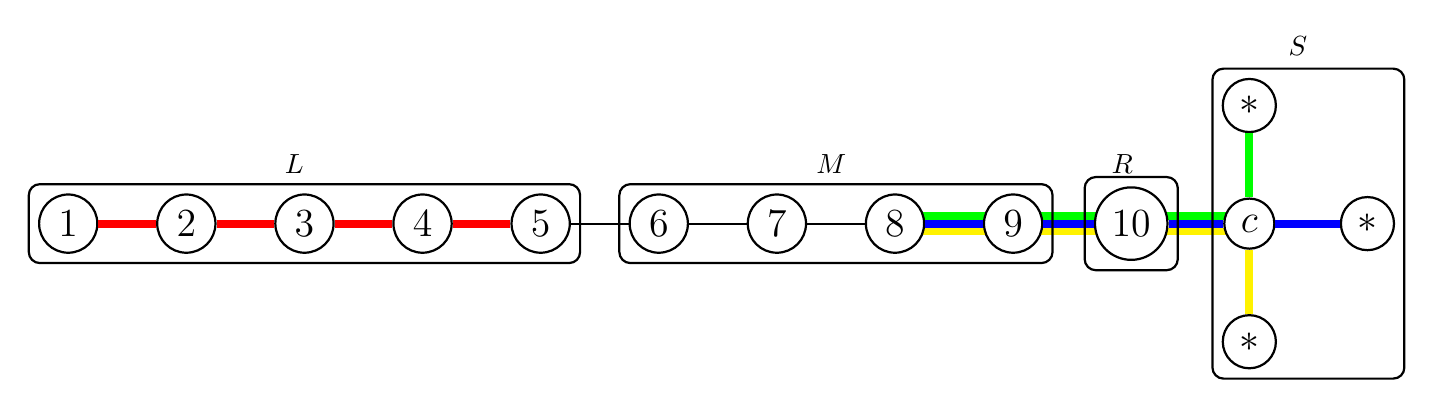
\begin{tikzpicture}[-,auto,node distance=1.5cm,
                    thick,main node/.style={circle,fill=white,draw,font=\sffamily\Large\bfseries}]

  \node[main node] (1) {$1$};
  \node[main node] (2) [right of=1] {$2$};
  \node[main node] (3) [right of=2] {$3$};
  \node[main node] (4) [right of=3] {$4$};
  \node[main node] (5) [right of=4] {$5$};
  \node[main node] (6) [right of=5]  {$6$};
  \node[main node] (7) [right of=6] {$7$};
  \node[main node] (8) [right of=7] {$8$};
  \node[main node] (9) [right of=8] {$9$};
  \node[main node] (10) [right of=9]  {$10$};
  \node[main node] (11) [right of=10]  {$c$};
  \node[main node] (12) [right of=11]  {$*$};
  \node[main node] (13) [above of=11]  {$*$};
  \node[main node] (14) [below of=11]  {$*$};
  

  \path[every node/.style={font=\sffamily}]
    (1) edge  (2)
    (2) edge (3)
    (3) edge (4)
    (4) edge (5)
    (5) edge (6)
    (6) edge (7)
    (7) edge (8)
    (8) edge (9)
    (9) edge (10)
    (10) edge (11)
    (11) edge (12)
    edge (13)
    edge (14);
      
     
   \draw[line width=1mm,color=red] (1) to (2) to (3) to (4) to (5);
   
   \draw [line width=1mm,color=blue] (11) to (12);
   \draw [line width=1mm,color=green] (11) to (13);
   \draw [line width=1mm,color=yellow] (11) to (14);
   \draw [line width=1mm,color=blue] (8) to (9) to (10) to (11);
   
   \node (LBox) [draw,rounded corners, fit= (1) (2) (3) (4) (5)] {};
   \node (MBox) [draw,rounded corners, fit= (6) (7) (8) (9)] {};
   \node (RBox) [draw,rounded corners, fit= (10)] {};
   \node (SBox) [draw,rounded corners, fit= (11) (12) (13) (14)] {};
   
   \node [above=0.5cm,text width=0.5cm] at (LBox) {$L$};
   \node [above=0.5cm,text width=0.5cm] at (MBox) {$M$};
   \node [above=0.5cm,text width=0.5cm] at (RBox) {$R$};
   \node [,above=2cm,text width=0.5cm] at (SBox) {$S$}; 
   
\begin{scope}[on background layer]
   \node[style={circle,,font=\sffamily\Large\bfseries}] (8H) at ($ (8) + (0,0.1) $) { };
   \node[style={circle,,font=\sffamily\Large\bfseries}] (9H) at ($ (9) + (0,0.1) $) { };   
   \node[style={circle,,font=\sffamily\Large\bfseries}] (10H) at ($ (10) + (0,0.1) $) { };
   \node[style={circle,,font=\sffamily\Large\bfseries}] (11H) at ($ (11) + (0,0.1) $) { };
   \draw [line width=1mm,color=green] (8H) to (9H) to (10H) to (11H);
   \node[style={circle,,font=\sffamily\Large\bfseries}] (8L) at ($ (8) + (0,-0.1) $) { };
   \node[style={circle,,font=\sffamily\Large\bfseries}] (9L) at ($ (9) + (0,-0.1) $) { };
   \node[style={circle,,font=\sffamily\Large\bfseries}] (10L) at ($ (10) + (0,-0.1) $) { };
   \node[style={circle,,font=\sffamily\Large\bfseries}] (11L) at ($ (11) + (0,-0.1) $) { };
   \draw [line width=1mm,color=yellow] (8L) to (9L) to (10L) to (11L);
\end{scope}
    
   
\end{tikzpicture}
}
\end{center}
\caption{The Naive Improvement on $S_{4}^{9}$ for $m=9$. The \textcolor{red}{red lines indicating the end-ensuring cycle $\{1,2,3,4,5,4,3,2,1 \}$} and the other coloured lines indicating the end-ensuring cycles, for each $*$, $\{*,c,10,9,8,9,10,c,* \}$ (as $\halflength=4$).}
\end{examplefigure}


Using the Naive Improvement Policy we can achieve an improvement over the Random Oscillation if $2(n+k) -nm \geq 0$ and get a bound of $V \geq \frac{2m}{2(n+k)+nm}$ (or $V \geq \frac{1}{n}$ if $M=\emptyset,R=\emptyset$), by choosing optimal $Q_{L}$ and $Q_{S}$ (See  appendix \ref{appendix:Naiveanalysis}).


\begin{myfigure}
\begin{center}
% Created by tikzDevice version 0.12 on 2019-02-23 16:14:03
% !TEX encoding = UTF-8 Unicode
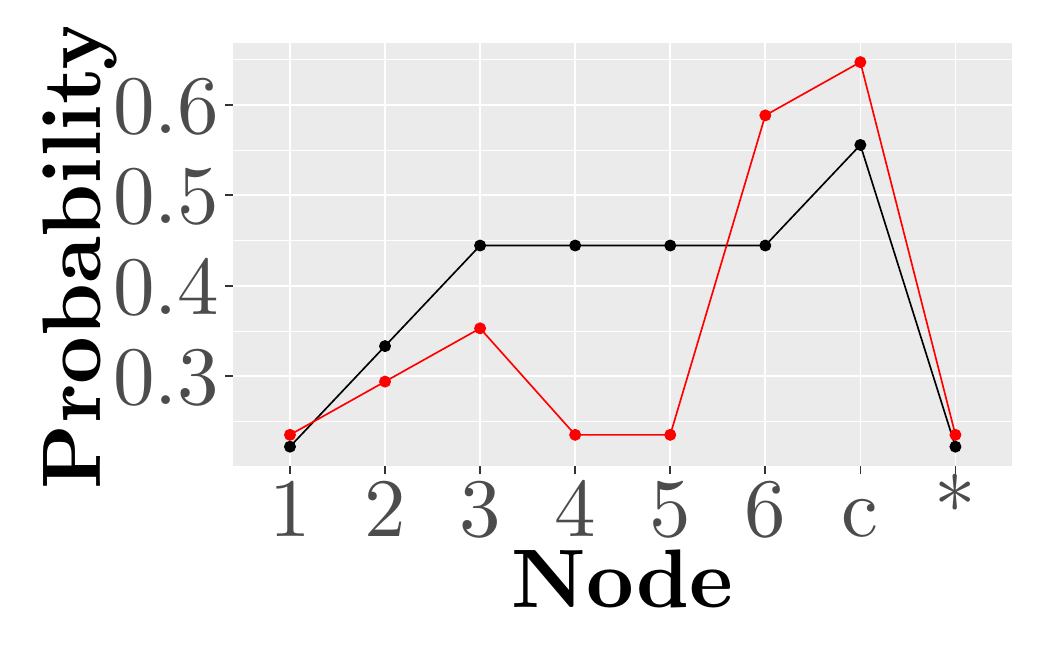
\begin{tikzpicture}[x=1pt,y=1pt]
\definecolor{fillColor}{RGB}{255,255,255}
\path[use as bounding box,fill=fillColor,fill opacity=0.00] (0,0) rectangle (361.35,216.81);
\begin{scope}
\path[clip] (  0.00,  0.00) rectangle (361.35,216.81);
\definecolor{drawColor}{RGB}{255,255,255}
\definecolor{fillColor}{RGB}{255,255,255}

\path[draw=drawColor,line width= 0.6pt,line join=round,line cap=round,fill=fillColor] (  0.00,  0.00) rectangle (361.35,216.81);
\end{scope}
\begin{scope}
\path[clip] ( 74.17, 58.45) rectangle (355.85,211.31);
\definecolor{fillColor}{gray}{0.92}

\path[fill=fillColor] ( 74.17, 58.45) rectangle (355.85,211.31);
\definecolor{drawColor}{RGB}{255,255,255}

\path[draw=drawColor,line width= 0.3pt,line join=round] ( 74.17, 74.49) --
	(355.85, 74.49);

\path[draw=drawColor,line width= 0.3pt,line join=round] ( 74.17,107.20) --
	(355.85,107.20);

\path[draw=drawColor,line width= 0.3pt,line join=round] ( 74.17,139.91) --
	(355.85,139.91);

\path[draw=drawColor,line width= 0.3pt,line join=round] ( 74.17,172.61) --
	(355.85,172.61);

\path[draw=drawColor,line width= 0.3pt,line join=round] ( 74.17,205.32) --
	(355.85,205.32);

\path[draw=drawColor,line width= 0.6pt,line join=round] ( 74.17, 90.84) --
	(355.85, 90.84);

\path[draw=drawColor,line width= 0.6pt,line join=round] ( 74.17,123.55) --
	(355.85,123.55);

\path[draw=drawColor,line width= 0.6pt,line join=round] ( 74.17,156.26) --
	(355.85,156.26);

\path[draw=drawColor,line width= 0.6pt,line join=round] ( 74.17,188.97) --
	(355.85,188.97);

\path[draw=drawColor,line width= 0.6pt,line join=round] ( 94.78, 58.45) --
	( 94.78,211.31);

\path[draw=drawColor,line width= 0.6pt,line join=round] (129.13, 58.45) --
	(129.13,211.31);

\path[draw=drawColor,line width= 0.6pt,line join=round] (163.48, 58.45) --
	(163.48,211.31);

\path[draw=drawColor,line width= 0.6pt,line join=round] (197.84, 58.45) --
	(197.84,211.31);

\path[draw=drawColor,line width= 0.6pt,line join=round] (232.19, 58.45) --
	(232.19,211.31);

\path[draw=drawColor,line width= 0.6pt,line join=round] (266.54, 58.45) --
	(266.54,211.31);

\path[draw=drawColor,line width= 0.6pt,line join=round] (300.89, 58.45) --
	(300.89,211.31);

\path[draw=drawColor,line width= 0.6pt,line join=round] (335.24, 58.45) --
	(335.24,211.31);
\definecolor{drawColor}{RGB}{0,0,0}
\definecolor{fillColor}{RGB}{0,0,0}

\path[draw=drawColor,line width= 0.4pt,line join=round,line cap=round,fill=fillColor] ( 94.78, 65.40) circle (  1.96);

\path[draw=drawColor,line width= 0.4pt,line join=round,line cap=round,fill=fillColor] (129.13,101.74) circle (  1.96);

\path[draw=drawColor,line width= 0.4pt,line join=round,line cap=round,fill=fillColor] (163.48,138.09) circle (  1.96);

\path[draw=drawColor,line width= 0.4pt,line join=round,line cap=round,fill=fillColor] (197.84,138.09) circle (  1.96);

\path[draw=drawColor,line width= 0.4pt,line join=round,line cap=round,fill=fillColor] (232.19,138.09) circle (  1.96);

\path[draw=drawColor,line width= 0.4pt,line join=round,line cap=round,fill=fillColor] (266.54,138.09) circle (  1.96);

\path[draw=drawColor,line width= 0.4pt,line join=round,line cap=round,fill=fillColor] (300.89,174.43) circle (  1.96);

\path[draw=drawColor,line width= 0.4pt,line join=round,line cap=round,fill=fillColor] (335.24, 65.40) circle (  1.96);

\path[draw=drawColor,line width= 0.6pt,line join=round] ( 94.78, 65.40) --
	(129.13,101.74) --
	(163.48,138.09) --
	(197.84,138.09) --
	(232.19,138.09) --
	(266.54,138.09) --
	(300.89,174.43) --
	(335.24, 65.40);
\definecolor{drawColor}{RGB}{255,0,0}
\definecolor{fillColor}{RGB}{255,0,0}

\path[draw=drawColor,line width= 0.4pt,line join=round,line cap=round,fill=fillColor] ( 94.78, 69.68) circle (  1.96);

\path[draw=drawColor,line width= 0.4pt,line join=round,line cap=round,fill=fillColor] (129.13, 88.92) circle (  1.96);

\path[draw=drawColor,line width= 0.4pt,line join=round,line cap=round,fill=fillColor] (163.48,108.16) circle (  1.96);

\path[draw=drawColor,line width= 0.4pt,line join=round,line cap=round,fill=fillColor] (197.84, 69.68) circle (  1.96);

\path[draw=drawColor,line width= 0.4pt,line join=round,line cap=round,fill=fillColor] (232.19, 69.68) circle (  1.96);

\path[draw=drawColor,line width= 0.4pt,line join=round,line cap=round,fill=fillColor] (266.54,185.12) circle (  1.96);

\path[draw=drawColor,line width= 0.4pt,line join=round,line cap=round,fill=fillColor] (300.89,204.36) circle (  1.96);

\path[draw=drawColor,line width= 0.4pt,line join=round,line cap=round,fill=fillColor] (335.24, 69.68) circle (  1.96);

\path[draw=drawColor,line width= 0.6pt,line join=round] ( 94.78, 69.68) --
	(129.13, 88.92) --
	(163.48,108.16) --
	(197.84, 69.68) --
	(232.19, 69.68) --
	(266.54,185.12) --
	(300.89,204.36) --
	(335.24, 69.68);
\end{scope}
\begin{scope}
\path[clip] (  0.00,  0.00) rectangle (361.35,216.81);
\definecolor{drawColor}{gray}{0.30}

\node[text=drawColor,anchor=base east,inner sep=0pt, outer sep=0pt, scale=  3.00] at ( 69.22, 80.51) {0.3};

\node[text=drawColor,anchor=base east,inner sep=0pt, outer sep=0pt, scale=  3.00] at ( 69.22,113.22) {0.4};

\node[text=drawColor,anchor=base east,inner sep=0pt, outer sep=0pt, scale=  3.00] at ( 69.22,145.93) {0.5};

\node[text=drawColor,anchor=base east,inner sep=0pt, outer sep=0pt, scale=  3.00] at ( 69.22,178.64) {0.6};
\end{scope}
\begin{scope}
\path[clip] (  0.00,  0.00) rectangle (361.35,216.81);
\definecolor{drawColor}{gray}{0.20}

\path[draw=drawColor,line width= 0.6pt,line join=round] ( 71.42, 90.84) --
	( 74.17, 90.84);

\path[draw=drawColor,line width= 0.6pt,line join=round] ( 71.42,123.55) --
	( 74.17,123.55);

\path[draw=drawColor,line width= 0.6pt,line join=round] ( 71.42,156.26) --
	( 74.17,156.26);

\path[draw=drawColor,line width= 0.6pt,line join=round] ( 71.42,188.97) --
	( 74.17,188.97);
\end{scope}
\begin{scope}
\path[clip] (  0.00,  0.00) rectangle (361.35,216.81);
\definecolor{drawColor}{gray}{0.20}

\path[draw=drawColor,line width= 0.6pt,line join=round] ( 94.78, 55.70) --
	( 94.78, 58.45);

\path[draw=drawColor,line width= 0.6pt,line join=round] (129.13, 55.70) --
	(129.13, 58.45);

\path[draw=drawColor,line width= 0.6pt,line join=round] (163.48, 55.70) --
	(163.48, 58.45);

\path[draw=drawColor,line width= 0.6pt,line join=round] (197.84, 55.70) --
	(197.84, 58.45);

\path[draw=drawColor,line width= 0.6pt,line join=round] (232.19, 55.70) --
	(232.19, 58.45);

\path[draw=drawColor,line width= 0.6pt,line join=round] (266.54, 55.70) --
	(266.54, 58.45);

\path[draw=drawColor,line width= 0.6pt,line join=round] (300.89, 55.70) --
	(300.89, 58.45);

\path[draw=drawColor,line width= 0.6pt,line join=round] (335.24, 55.70) --
	(335.24, 58.45);
\end{scope}
\begin{scope}
\path[clip] (  0.00,  0.00) rectangle (361.35,216.81);
\definecolor{drawColor}{gray}{0.30}

\node[text=drawColor,anchor=base,inner sep=0pt, outer sep=0pt, scale=  3.00] at ( 94.78, 32.84) {1};

\node[text=drawColor,anchor=base,inner sep=0pt, outer sep=0pt, scale=  3.00] at (129.13, 32.84) {2};

\node[text=drawColor,anchor=base,inner sep=0pt, outer sep=0pt, scale=  3.00] at (163.48, 32.84) {3};

\node[text=drawColor,anchor=base,inner sep=0pt, outer sep=0pt, scale=  3.00] at (197.84, 32.84) {4};

\node[text=drawColor,anchor=base,inner sep=0pt, outer sep=0pt, scale=  3.00] at (232.19, 32.84) {5};

\node[text=drawColor,anchor=base,inner sep=0pt, outer sep=0pt, scale=  3.00] at (266.54, 32.84) {6};

\node[text=drawColor,anchor=base,inner sep=0pt, outer sep=0pt, scale=  3.00] at (300.89, 32.84) {c};

\node[text=drawColor,anchor=base,inner sep=0pt, outer sep=0pt, scale=  3.00] at (335.24, 32.84) {*};
\end{scope}
\begin{scope}
\path[clip] (  0.00,  0.00) rectangle (361.35,216.81);
\definecolor{drawColor}{RGB}{0,0,0}

\node[text=drawColor,anchor=base,inner sep=0pt, outer sep=0pt, scale=  3.00] at (215.01,  7.44) {\bfseries Node};
\end{scope}
\begin{scope}
\path[clip] (  0.00,  0.00) rectangle (361.35,216.81);
\definecolor{drawColor}{RGB}{0,0,0}

\node[text=drawColor,rotate= 90.00,anchor=base,inner sep=0pt, outer sep=0pt, scale=  3.00] at ( 26.20,134.88) {\bfseries Probability};
\end{scope}
\end{tikzpicture}

\end{center}
\caption{Interception probabilities of $S^5_{4}$ when $m=4$, with the \textcolor{red}{red Probabilities showing the Naive Improvement Policy $\alpha \left(\frac{2}{17},\frac{6}{17} \right)$}.}
\end{myfigure}



\textbf{A Combinatorial Improvement}
Let $\bm{\pi}=\beta(Q_{L},Q_{S})$ denote the Combinatorial Improvement Policy.
As before the end-ensuring cycle, $\{ 1,...,\floor{\frac{m}{2}}+1,...,1 \}$ is played with probability $Q_{L}$, so $q_{L}=Q_{L}$. Also;

\begin{enumerate}
\item[Case i)] If $R \neq \emptyset$ then $\floor{\frac{m}{2}}=n+r$, for some excess $r$. Then form an end-ensuring cycle on the nodes $\{ n+k+1-\floor{\frac{m}{2}},...,k+1,c,*,c,*,...,c,*,c,k+1,...,n+k+1-\floor{\frac{m}{2}} \}$, this is of length $2(n-\floor{\frac{m}{2}}+1)+2(n-1)=4n-2 \frac{m}{2}=4n-2(n+r)=2n+2r=2 \floor{\frac{m}{2}} \leq m$ (so are end-ensuring). This cycle will be played with probability $Q_{S}$ and improves all the nodes in $R$ (non-increasing) and $S$($c$ is better than $*$) so $q_{R}=Q_{R}$ and $q_{S}=Q_{S}$.

\item[Case ii)] If $R = \emptyset$ then an end-ensuring cycle is formed by choosing $\halflength$ $*$ nodes each equally likely. This construction is performed with probability $Q_{S}$ and nodes in $S$ ($c$ is better than $*$). The actually improvement made is $$q_{S}=Q_{S} \times \mathbb{P}(\text{A particular } * \text{ node is picked})=Q_{S} \times \frac{\floor{\frac{m}{2}}}{n-1} $$
\end{enumerate}
To distinguish between the cases we shall label case i) $\beta_{1}$ and case ii) $\beta_{2}$.

Using the Choosing Improvement Policy we can achieve an improvement over the Random Oscillation in both cases (under some conditions) and get a lower bound. (See  appendix \ref{appendix:Choosinganalysis})


\begin{myfigure}
\begin{center}
% Created by tikzDevice version 0.10.1 on 2017-11-24 11:28:21
% !TEX encoding = UTF-8 Unicode
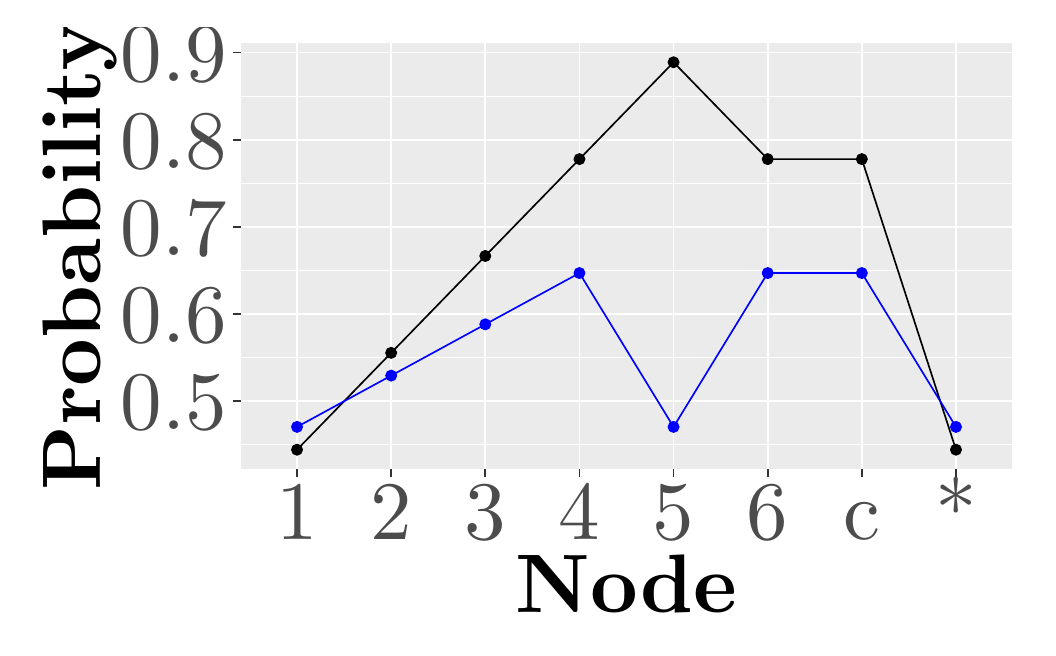
\begin{tikzpicture}[x=1pt,y=1pt]
\definecolor{fillColor}{RGB}{255,255,255}
\path[use as bounding box,fill=fillColor,fill opacity=0.00] (0,0) rectangle (361.35,216.81);
\begin{scope}
\path[clip] (  0.00,  0.00) rectangle (361.35,216.81);
\definecolor{drawColor}{RGB}{255,255,255}
\definecolor{fillColor}{RGB}{255,255,255}

\path[draw=drawColor,line width= 0.6pt,line join=round,line cap=round,fill=fillColor] (  0.00,  0.00) rectangle (361.35,216.81);
\end{scope}
\begin{scope}
\path[clip] ( 76.92, 57.31) rectangle (355.85,211.31);
\definecolor{fillColor}{gray}{0.92}

\path[fill=fillColor] ( 76.92, 57.31) rectangle (355.85,211.31);
\definecolor{drawColor}{RGB}{255,255,255}

\path[draw=drawColor,line width= 0.3pt,line join=round] ( 76.92, 66.06) --
	(355.85, 66.06);

\path[draw=drawColor,line width= 0.3pt,line join=round] ( 76.92, 97.56) --
	(355.85, 97.56);

\path[draw=drawColor,line width= 0.3pt,line join=round] ( 76.92,129.06) --
	(355.85,129.06);

\path[draw=drawColor,line width= 0.3pt,line join=round] ( 76.92,160.56) --
	(355.85,160.56);

\path[draw=drawColor,line width= 0.3pt,line join=round] ( 76.92,192.06) --
	(355.85,192.06);

\path[draw=drawColor,line width= 0.6pt,line join=round] ( 76.92, 81.81) --
	(355.85, 81.81);

\path[draw=drawColor,line width= 0.6pt,line join=round] ( 76.92,113.31) --
	(355.85,113.31);

\path[draw=drawColor,line width= 0.6pt,line join=round] ( 76.92,144.81) --
	(355.85,144.81);

\path[draw=drawColor,line width= 0.6pt,line join=round] ( 76.92,176.31) --
	(355.85,176.31);

\path[draw=drawColor,line width= 0.6pt,line join=round] ( 76.92,207.81) --
	(355.85,207.81);

\path[draw=drawColor,line width= 0.6pt,line join=round] ( 97.33, 57.31) --
	( 97.33,211.31);

\path[draw=drawColor,line width= 0.6pt,line join=round] (131.35, 57.31) --
	(131.35,211.31);

\path[draw=drawColor,line width= 0.6pt,line join=round] (165.36, 57.31) --
	(165.36,211.31);

\path[draw=drawColor,line width= 0.6pt,line join=round] (199.38, 57.31) --
	(199.38,211.31);

\path[draw=drawColor,line width= 0.6pt,line join=round] (233.39, 57.31) --
	(233.39,211.31);

\path[draw=drawColor,line width= 0.6pt,line join=round] (267.41, 57.31) --
	(267.41,211.31);

\path[draw=drawColor,line width= 0.6pt,line join=round] (301.42, 57.31) --
	(301.42,211.31);

\path[draw=drawColor,line width= 0.6pt,line join=round] (335.44, 57.31) --
	(335.44,211.31);
\definecolor{drawColor}{RGB}{0,0,0}
\definecolor{fillColor}{RGB}{0,0,0}

\path[draw=drawColor,line width= 0.4pt,line join=round,line cap=round,fill=fillColor] ( 97.33, 64.31) circle (  1.96);

\path[draw=drawColor,line width= 0.4pt,line join=round,line cap=round,fill=fillColor] (131.35, 99.31) circle (  1.96);

\path[draw=drawColor,line width= 0.4pt,line join=round,line cap=round,fill=fillColor] (165.36,134.31) circle (  1.96);

\path[draw=drawColor,line width= 0.4pt,line join=round,line cap=round,fill=fillColor] (199.38,169.31) circle (  1.96);

\path[draw=drawColor,line width= 0.4pt,line join=round,line cap=round,fill=fillColor] (233.39,204.31) circle (  1.96);

\path[draw=drawColor,line width= 0.4pt,line join=round,line cap=round,fill=fillColor] (267.41,169.31) circle (  1.96);

\path[draw=drawColor,line width= 0.4pt,line join=round,line cap=round,fill=fillColor] (301.42,169.31) circle (  1.96);

\path[draw=drawColor,line width= 0.4pt,line join=round,line cap=round,fill=fillColor] (335.44, 64.31) circle (  1.96);

\path[draw=drawColor,line width= 0.6pt,line join=round] ( 97.33, 64.31) --
	(131.35, 99.31) --
	(165.36,134.31) --
	(199.38,169.31) --
	(233.39,204.31) --
	(267.41,169.31) --
	(301.42,169.31) --
	(335.44, 64.31);
\definecolor{drawColor}{RGB}{0,0,255}
\definecolor{fillColor}{RGB}{0,0,255}

\path[draw=drawColor,line width= 0.4pt,line join=round,line cap=round,fill=fillColor] ( 97.33, 72.55) circle (  1.96);

\path[draw=drawColor,line width= 0.4pt,line join=round,line cap=round,fill=fillColor] (131.35, 91.08) circle (  1.96);

\path[draw=drawColor,line width= 0.4pt,line join=round,line cap=round,fill=fillColor] (165.36,109.61) circle (  1.96);

\path[draw=drawColor,line width= 0.4pt,line join=round,line cap=round,fill=fillColor] (199.38,128.14) circle (  1.96);

\path[draw=drawColor,line width= 0.4pt,line join=round,line cap=round,fill=fillColor] (233.39, 72.55) circle (  1.96);

\path[draw=drawColor,line width= 0.4pt,line join=round,line cap=round,fill=fillColor] (267.41,128.14) circle (  1.96);

\path[draw=drawColor,line width= 0.4pt,line join=round,line cap=round,fill=fillColor] (301.42,128.14) circle (  1.96);

\path[draw=drawColor,line width= 0.4pt,line join=round,line cap=round,fill=fillColor] (335.44, 72.55) circle (  1.96);

\path[draw=drawColor,line width= 0.6pt,line join=round] ( 97.33, 72.55) --
	(131.35, 91.08) --
	(165.36,109.61) --
	(199.38,128.14) --
	(233.39, 72.55) --
	(267.41,128.14) --
	(301.42,128.14) --
	(335.44, 72.55);
\end{scope}
\begin{scope}
\path[clip] (  0.00,  0.00) rectangle (361.35,216.81);
\definecolor{drawColor}{gray}{0.30}

\node[text=drawColor,anchor=base east,inner sep=0pt, outer sep=0pt, scale=  3.00] at ( 71.97, 71.48) {0.5};

\node[text=drawColor,anchor=base east,inner sep=0pt, outer sep=0pt, scale=  3.00] at ( 71.97,102.98) {0.6};

\node[text=drawColor,anchor=base east,inner sep=0pt, outer sep=0pt, scale=  3.00] at ( 71.97,134.48) {0.7};

\node[text=drawColor,anchor=base east,inner sep=0pt, outer sep=0pt, scale=  3.00] at ( 71.97,165.98) {0.8};

\node[text=drawColor,anchor=base east,inner sep=0pt, outer sep=0pt, scale=  3.00] at ( 71.97,197.48) {0.9};
\end{scope}
\begin{scope}
\path[clip] (  0.00,  0.00) rectangle (361.35,216.81);
\definecolor{drawColor}{gray}{0.20}

\path[draw=drawColor,line width= 0.6pt,line join=round] ( 74.17, 81.81) --
	( 76.92, 81.81);

\path[draw=drawColor,line width= 0.6pt,line join=round] ( 74.17,113.31) --
	( 76.92,113.31);

\path[draw=drawColor,line width= 0.6pt,line join=round] ( 74.17,144.81) --
	( 76.92,144.81);

\path[draw=drawColor,line width= 0.6pt,line join=round] ( 74.17,176.31) --
	( 76.92,176.31);

\path[draw=drawColor,line width= 0.6pt,line join=round] ( 74.17,207.81) --
	( 76.92,207.81);
\end{scope}
\begin{scope}
\path[clip] (  0.00,  0.00) rectangle (361.35,216.81);
\definecolor{drawColor}{gray}{0.20}

\path[draw=drawColor,line width= 0.6pt,line join=round] ( 97.33, 54.56) --
	( 97.33, 57.31);

\path[draw=drawColor,line width= 0.6pt,line join=round] (131.35, 54.56) --
	(131.35, 57.31);

\path[draw=drawColor,line width= 0.6pt,line join=round] (165.36, 54.56) --
	(165.36, 57.31);

\path[draw=drawColor,line width= 0.6pt,line join=round] (199.38, 54.56) --
	(199.38, 57.31);

\path[draw=drawColor,line width= 0.6pt,line join=round] (233.39, 54.56) --
	(233.39, 57.31);

\path[draw=drawColor,line width= 0.6pt,line join=round] (267.41, 54.56) --
	(267.41, 57.31);

\path[draw=drawColor,line width= 0.6pt,line join=round] (301.42, 54.56) --
	(301.42, 57.31);

\path[draw=drawColor,line width= 0.6pt,line join=round] (335.44, 54.56) --
	(335.44, 57.31);
\end{scope}
\begin{scope}
\path[clip] (  0.00,  0.00) rectangle (361.35,216.81);
\definecolor{drawColor}{gray}{0.30}

\node[text=drawColor,anchor=base,inner sep=0pt, outer sep=0pt, scale=  3.00] at ( 97.33, 31.70) {1};

\node[text=drawColor,anchor=base,inner sep=0pt, outer sep=0pt, scale=  3.00] at (131.35, 31.70) {2};

\node[text=drawColor,anchor=base,inner sep=0pt, outer sep=0pt, scale=  3.00] at (165.36, 31.70) {3};

\node[text=drawColor,anchor=base,inner sep=0pt, outer sep=0pt, scale=  3.00] at (199.38, 31.70) {4};

\node[text=drawColor,anchor=base,inner sep=0pt, outer sep=0pt, scale=  3.00] at (233.39, 31.70) {5};

\node[text=drawColor,anchor=base,inner sep=0pt, outer sep=0pt, scale=  3.00] at (267.41, 31.70) {6};

\node[text=drawColor,anchor=base,inner sep=0pt, outer sep=0pt, scale=  3.00] at (301.42, 31.70) {c};

\node[text=drawColor,anchor=base,inner sep=0pt, outer sep=0pt, scale=  3.00] at (335.44, 31.70) {*};
\end{scope}
\begin{scope}
\path[clip] (  0.00,  0.00) rectangle (361.35,216.81);
\definecolor{drawColor}{RGB}{0,0,0}

\node[text=drawColor,anchor=base,inner sep=0pt, outer sep=0pt, scale=  3.00] at (216.39,  5.50) {\bfseries Node};
\end{scope}
\begin{scope}
\path[clip] (  0.00,  0.00) rectangle (361.35,216.81);
\definecolor{drawColor}{RGB}{0,0,0}

\node[text=drawColor,rotate= 90.00,anchor=base,inner sep=0pt, outer sep=0pt, scale=  3.00] at ( 26.20,134.31) {\bfseries Probability};
\end{scope}
\end{tikzpicture}

\end{center}
\caption{Interception probabilities of $S^5_{4}$ when $m=8$, with the \textcolor{blue}{blue Probabilities showing the Choosing Improvement Policy $\beta_{1} \left(\frac{2}{13},\frac{2}{13} \right)$}.}
\end{myfigure}



\begin{myfigure}
\begin{center}
% Created by tikzDevice version 0.10.1 on 2017-11-24 11:28:27
% !TEX encoding = UTF-8 Unicode
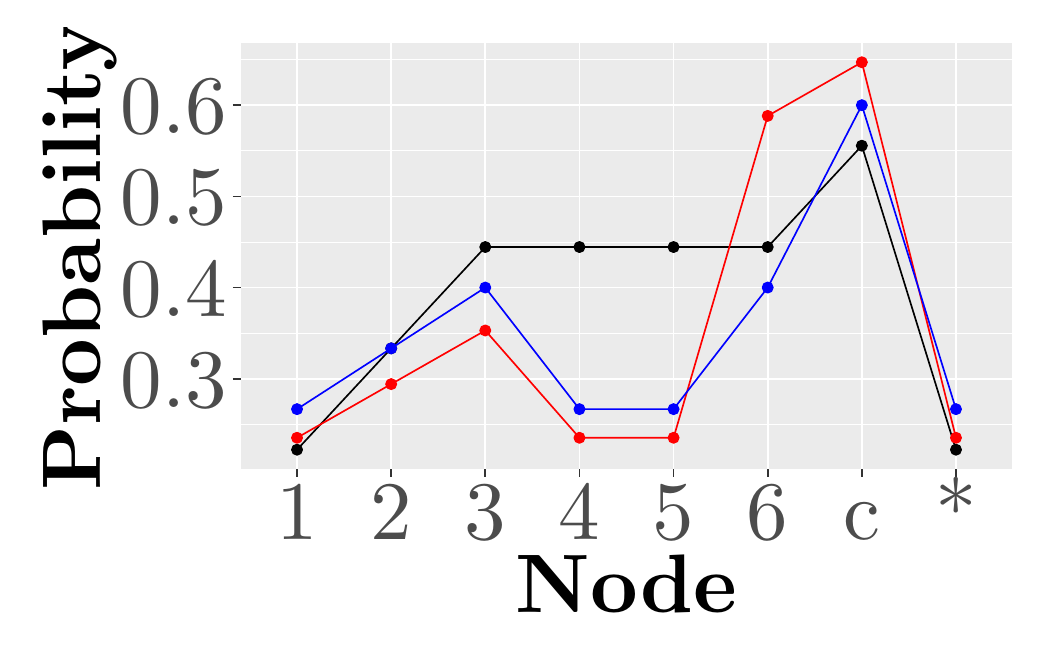
\begin{tikzpicture}[x=1pt,y=1pt]
\definecolor{fillColor}{RGB}{255,255,255}
\path[use as bounding box,fill=fillColor,fill opacity=0.00] (0,0) rectangle (361.35,216.81);
\begin{scope}
\path[clip] (  0.00,  0.00) rectangle (361.35,216.81);
\definecolor{drawColor}{RGB}{255,255,255}
\definecolor{fillColor}{RGB}{255,255,255}

\path[draw=drawColor,line width= 0.6pt,line join=round,line cap=round,fill=fillColor] (  0.00,  0.00) rectangle (361.35,216.81);
\end{scope}
\begin{scope}
\path[clip] ( 76.92, 57.31) rectangle (355.85,211.31);
\definecolor{fillColor}{gray}{0.92}

\path[fill=fillColor] ( 76.92, 57.31) rectangle (355.85,211.31);
\definecolor{drawColor}{RGB}{255,255,255}

\path[draw=drawColor,line width= 0.3pt,line join=round] ( 76.92, 73.47) --
	(355.85, 73.47);

\path[draw=drawColor,line width= 0.3pt,line join=round] ( 76.92,106.42) --
	(355.85,106.42);

\path[draw=drawColor,line width= 0.3pt,line join=round] ( 76.92,139.37) --
	(355.85,139.37);

\path[draw=drawColor,line width= 0.3pt,line join=round] ( 76.92,172.33) --
	(355.85,172.33);

\path[draw=drawColor,line width= 0.3pt,line join=round] ( 76.92,205.28) --
	(355.85,205.28);

\path[draw=drawColor,line width= 0.6pt,line join=round] ( 76.92, 89.94) --
	(355.85, 89.94);

\path[draw=drawColor,line width= 0.6pt,line join=round] ( 76.92,122.90) --
	(355.85,122.90);

\path[draw=drawColor,line width= 0.6pt,line join=round] ( 76.92,155.85) --
	(355.85,155.85);

\path[draw=drawColor,line width= 0.6pt,line join=round] ( 76.92,188.80) --
	(355.85,188.80);

\path[draw=drawColor,line width= 0.6pt,line join=round] ( 97.33, 57.31) --
	( 97.33,211.31);

\path[draw=drawColor,line width= 0.6pt,line join=round] (131.35, 57.31) --
	(131.35,211.31);

\path[draw=drawColor,line width= 0.6pt,line join=round] (165.36, 57.31) --
	(165.36,211.31);

\path[draw=drawColor,line width= 0.6pt,line join=round] (199.38, 57.31) --
	(199.38,211.31);

\path[draw=drawColor,line width= 0.6pt,line join=round] (233.39, 57.31) --
	(233.39,211.31);

\path[draw=drawColor,line width= 0.6pt,line join=round] (267.41, 57.31) --
	(267.41,211.31);

\path[draw=drawColor,line width= 0.6pt,line join=round] (301.42, 57.31) --
	(301.42,211.31);

\path[draw=drawColor,line width= 0.6pt,line join=round] (335.44, 57.31) --
	(335.44,211.31);
\definecolor{drawColor}{RGB}{0,0,0}
\definecolor{fillColor}{RGB}{0,0,0}

\path[draw=drawColor,line width= 0.4pt,line join=round,line cap=round,fill=fillColor] ( 97.33, 64.31) circle (  1.96);

\path[draw=drawColor,line width= 0.4pt,line join=round,line cap=round,fill=fillColor] (131.35,100.93) circle (  1.96);

\path[draw=drawColor,line width= 0.4pt,line join=round,line cap=round,fill=fillColor] (165.36,137.54) circle (  1.96);

\path[draw=drawColor,line width= 0.4pt,line join=round,line cap=round,fill=fillColor] (199.38,137.54) circle (  1.96);

\path[draw=drawColor,line width= 0.4pt,line join=round,line cap=round,fill=fillColor] (233.39,137.54) circle (  1.96);

\path[draw=drawColor,line width= 0.4pt,line join=round,line cap=round,fill=fillColor] (267.41,137.54) circle (  1.96);

\path[draw=drawColor,line width= 0.4pt,line join=round,line cap=round,fill=fillColor] (301.42,174.16) circle (  1.96);

\path[draw=drawColor,line width= 0.4pt,line join=round,line cap=round,fill=fillColor] (335.44, 64.31) circle (  1.96);

\path[draw=drawColor,line width= 0.6pt,line join=round] ( 97.33, 64.31) --
	(131.35,100.93) --
	(165.36,137.54) --
	(199.38,137.54) --
	(233.39,137.54) --
	(267.41,137.54) --
	(301.42,174.16) --
	(335.44, 64.31);
\definecolor{drawColor}{RGB}{255,0,0}
\definecolor{fillColor}{RGB}{255,0,0}

\path[draw=drawColor,line width= 0.4pt,line join=round,line cap=round,fill=fillColor] ( 97.33, 68.62) circle (  1.96);

\path[draw=drawColor,line width= 0.4pt,line join=round,line cap=round,fill=fillColor] (131.35, 88.01) circle (  1.96);

\path[draw=drawColor,line width= 0.4pt,line join=round,line cap=round,fill=fillColor] (165.36,107.39) circle (  1.96);

\path[draw=drawColor,line width= 0.4pt,line join=round,line cap=round,fill=fillColor] (199.38, 68.62) circle (  1.96);

\path[draw=drawColor,line width= 0.4pt,line join=round,line cap=round,fill=fillColor] (233.39, 68.62) circle (  1.96);

\path[draw=drawColor,line width= 0.4pt,line join=round,line cap=round,fill=fillColor] (267.41,184.93) circle (  1.96);

\path[draw=drawColor,line width= 0.4pt,line join=round,line cap=round,fill=fillColor] (301.42,204.31) circle (  1.96);

\path[draw=drawColor,line width= 0.4pt,line join=round,line cap=round,fill=fillColor] (335.44, 68.62) circle (  1.96);

\path[draw=drawColor,line width= 0.6pt,line join=round] ( 97.33, 68.62) --
	(131.35, 88.01) --
	(165.36,107.39) --
	(199.38, 68.62) --
	(233.39, 68.62) --
	(267.41,184.93) --
	(301.42,204.31) --
	(335.44, 68.62);
\definecolor{drawColor}{RGB}{0,0,255}
\definecolor{fillColor}{RGB}{0,0,255}

\path[draw=drawColor,line width= 0.4pt,line join=round,line cap=round,fill=fillColor] ( 97.33, 78.96) circle (  1.96);

\path[draw=drawColor,line width= 0.4pt,line join=round,line cap=round,fill=fillColor] (131.35,100.93) circle (  1.96);

\path[draw=drawColor,line width= 0.4pt,line join=round,line cap=round,fill=fillColor] (165.36,122.90) circle (  1.96);

\path[draw=drawColor,line width= 0.4pt,line join=round,line cap=round,fill=fillColor] (199.38, 78.96) circle (  1.96);

\path[draw=drawColor,line width= 0.4pt,line join=round,line cap=round,fill=fillColor] (233.39, 78.96) circle (  1.96);

\path[draw=drawColor,line width= 0.4pt,line join=round,line cap=round,fill=fillColor] (267.41,122.90) circle (  1.96);

\path[draw=drawColor,line width= 0.4pt,line join=round,line cap=round,fill=fillColor] (301.42,188.80) circle (  1.96);

\path[draw=drawColor,line width= 0.4pt,line join=round,line cap=round,fill=fillColor] (335.44, 78.96) circle (  1.96);

\path[draw=drawColor,line width= 0.6pt,line join=round] ( 97.33, 78.96) --
	(131.35,100.93) --
	(165.36,122.90) --
	(199.38, 78.96) --
	(233.39, 78.96) --
	(267.41,122.90) --
	(301.42,188.80) --
	(335.44, 78.96);
\end{scope}
\begin{scope}
\path[clip] (  0.00,  0.00) rectangle (361.35,216.81);
\definecolor{drawColor}{gray}{0.30}

\node[text=drawColor,anchor=base east,inner sep=0pt, outer sep=0pt, scale=  3.00] at ( 71.97, 79.61) {0.3};

\node[text=drawColor,anchor=base east,inner sep=0pt, outer sep=0pt, scale=  3.00] at ( 71.97,112.57) {0.4};

\node[text=drawColor,anchor=base east,inner sep=0pt, outer sep=0pt, scale=  3.00] at ( 71.97,145.52) {0.5};

\node[text=drawColor,anchor=base east,inner sep=0pt, outer sep=0pt, scale=  3.00] at ( 71.97,178.47) {0.6};
\end{scope}
\begin{scope}
\path[clip] (  0.00,  0.00) rectangle (361.35,216.81);
\definecolor{drawColor}{gray}{0.20}

\path[draw=drawColor,line width= 0.6pt,line join=round] ( 74.17, 89.94) --
	( 76.92, 89.94);

\path[draw=drawColor,line width= 0.6pt,line join=round] ( 74.17,122.90) --
	( 76.92,122.90);

\path[draw=drawColor,line width= 0.6pt,line join=round] ( 74.17,155.85) --
	( 76.92,155.85);

\path[draw=drawColor,line width= 0.6pt,line join=round] ( 74.17,188.80) --
	( 76.92,188.80);
\end{scope}
\begin{scope}
\path[clip] (  0.00,  0.00) rectangle (361.35,216.81);
\definecolor{drawColor}{gray}{0.20}

\path[draw=drawColor,line width= 0.6pt,line join=round] ( 97.33, 54.56) --
	( 97.33, 57.31);

\path[draw=drawColor,line width= 0.6pt,line join=round] (131.35, 54.56) --
	(131.35, 57.31);

\path[draw=drawColor,line width= 0.6pt,line join=round] (165.36, 54.56) --
	(165.36, 57.31);

\path[draw=drawColor,line width= 0.6pt,line join=round] (199.38, 54.56) --
	(199.38, 57.31);

\path[draw=drawColor,line width= 0.6pt,line join=round] (233.39, 54.56) --
	(233.39, 57.31);

\path[draw=drawColor,line width= 0.6pt,line join=round] (267.41, 54.56) --
	(267.41, 57.31);

\path[draw=drawColor,line width= 0.6pt,line join=round] (301.42, 54.56) --
	(301.42, 57.31);

\path[draw=drawColor,line width= 0.6pt,line join=round] (335.44, 54.56) --
	(335.44, 57.31);
\end{scope}
\begin{scope}
\path[clip] (  0.00,  0.00) rectangle (361.35,216.81);
\definecolor{drawColor}{gray}{0.30}

\node[text=drawColor,anchor=base,inner sep=0pt, outer sep=0pt, scale=  3.00] at ( 97.33, 31.70) {1};

\node[text=drawColor,anchor=base,inner sep=0pt, outer sep=0pt, scale=  3.00] at (131.35, 31.70) {2};

\node[text=drawColor,anchor=base,inner sep=0pt, outer sep=0pt, scale=  3.00] at (165.36, 31.70) {3};

\node[text=drawColor,anchor=base,inner sep=0pt, outer sep=0pt, scale=  3.00] at (199.38, 31.70) {4};

\node[text=drawColor,anchor=base,inner sep=0pt, outer sep=0pt, scale=  3.00] at (233.39, 31.70) {5};

\node[text=drawColor,anchor=base,inner sep=0pt, outer sep=0pt, scale=  3.00] at (267.41, 31.70) {6};

\node[text=drawColor,anchor=base,inner sep=0pt, outer sep=0pt, scale=  3.00] at (301.42, 31.70) {c};

\node[text=drawColor,anchor=base,inner sep=0pt, outer sep=0pt, scale=  3.00] at (335.44, 31.70) {*};
\end{scope}
\begin{scope}
\path[clip] (  0.00,  0.00) rectangle (361.35,216.81);
\definecolor{drawColor}{RGB}{0,0,0}

\node[text=drawColor,anchor=base,inner sep=0pt, outer sep=0pt, scale=  3.00] at (216.39,  5.50) {\bfseries Node};
\end{scope}
\begin{scope}
\path[clip] (  0.00,  0.00) rectangle (361.35,216.81);
\definecolor{drawColor}{RGB}{0,0,0}

\node[text=drawColor,rotate= 90.00,anchor=base,inner sep=0pt, outer sep=0pt, scale=  3.00] at ( 26.20,134.31) {\bfseries Probability};
\end{scope}
\end{tikzpicture}

\end{center}
\caption{Interception probabilities of $S^5_{4}$ when $m=4$, with the \textcolor{red}{red Probabilities showing the Naive Improvement Policy $\alpha \left(\frac{2}{17},\frac{6}{17} \right)$} and the \textcolor{blue}{blue Probabilities showing the Choosing Improvement Policy $\beta_{2} \left(\frac{1}{7},\frac{3}{14} \right)$}.}
\end{myfigure}


\subsection{Solution for $m=2k+1$ and $m=2k$}

\textbf{Solution for $m=2k+1$}

We will now present the solution for $m=2k+1$ which will depend on the comparison of $m$ to $2(n-1)$.

Let us first consider the case of $m \leq 2(n-1)$.
The patroller can look at the decomposition into $S_{n-1}$ and $L_{k+1}$ giving $V \geq \frac{1}{\frac{1}{V(S_{n-1})}+\frac{1}{V(L_{k+1})}}=\frac{1}{1+\frac{2(n-1)}{2k+1}}=\frac{2k+1}{2k+1+2(n-1)}=\frac{m}{m+2(n-1)}$.

We suggest that the attacker can `augment' their time-delayed strategy, this can be done by placing attacks at times $\tau,...,\tau+2k$ at the elongated node and times $\tau+k,\tau+k+1$ (or $k-1,k$ is proposed to work just as well), giving the bound $V \leq \frac{2k+1}{2k+1+2(n-1)}=\frac{m}{m+2(n-1)}$.

Hence giving $V=\frac{m}{m+2(n-1)}$.

Proof of `augmented' time-delayed strategy: NEEDED TO BE COMPLETE (IDEA: follows the same logic as the time-delayed strategy, the patroller cannot get more than $m$ attacks)

In the case of $m > 2(n-1)$.
The patroller can use the combinatorial improvement with $R=\emptyset$ , $M=\emptyset$, giving the bound $V \leq \frac{\floor{\frac{m}{2}}}{\floor{\frac{m}{2}}+n-1} = \frac{2k}{2k+2(n-1)}$

Note. Different decompositions give a worse bound. eg. into $S_{n}$,$L_{k}$ give $V \geq \frac{m}{m+2n}=\frac{2k+1}{2k+1+2n}$ (This has yet to be formally proved, but from this even if it is possible to get not 1 value for the star, then the bottom of the fraction is worse than this, and even this doesn't beat the combinatorial improvement)

The attacker again `augments' their time-delayed attack on to place attacks at times $0,...,2k-1$ at the elongated node and times $k-1,k$ at normal external nodes, giving the bound $V \geq \frac{2k}{2k+2(n-1)}$.

Hence giving $V=\frac{2k}{2k+2(n-1)}=\frac{m-1}{m-1+2(n-1)}$

Proof of `augmented' time-delayed strategy: NEEDED TO BE COMPLETE (IDEA: follows the same logic as the time-delayed strategy, the patroller cannot get more than $2k$ attacks)

So we know that the solution in the region of $m \leq 2(n-1)$ is higher than the solution in the region of $m > 2(n-1)$

\textbf{Solution for $m=2k$}

Here we will notice that we can follow the above, the patroller has both the decomposition into $S_{n-1}$,$L_{k+1}$ (available only if $m \leq 2(n-1)$) and the combinatorial improvement (Always available) giving the same bound of $V \geq \frac{2k}{2k+2(n-1)}=\frac{m}{m+2(n-1)}$.

The patroller as above can use an `augmented' version of the time-delayed strategy 

\subsection{Solution for $m=2k-1$ and $m=2k-2$}
First we will note that $M \neq \emptyset$

\textbf{Solution for $m=2k-1$}
As before it is assumed that it will matter on our comparison of $m$ to $2(n-1)$.

\textbf{when $m \geq 2n-1$}
If $m \geq 2n-1$ then $R \neq \emptyset$ we can use the combinatorial bound to get $V \geq \frac{m}{n+k+m}=\frac{2k-1}{n+3k-1}$. We note that this improvement is only possible if $m \leq n+k$ i.e $2k-1 \leq n+k$ so $k \leq n+1$. so $m=2k-1 \leq 2n+1$ which means we are only allowed to use this improvement in the region where $2k-1=2n-1, 2n+1$ i.e $k=n,n+1$.

We will then consider both cases

\textbf{for $k=n$}
If $k=n$ then the bound is $V \geq \frac{2n-1}{4n-1}$, we claim in this case that this is the same as using the decomposition to $L_{k}=L_{n}$ and $S_{n}$ getting us a bound of $V \geq \frac{1}{1+\frac{2n}{2n-1}}=\frac{2n-1}{4n-1}$.

Now the attacker requires an augmentation to there strategy

\textbf{for $k=n+1$}
If $k=n+1$ then the bound is $V \geq \frac{2n+1}{4n+2}$

The attacker should augment their attacks to simply place only $2(k-1)$ at the elongated node and $2(n-1)$ time centered around the centre node ($2$ for each external node). This will give a bound of $V \leq \frac{2(k-1)}{2(k-1)+2(n-1)}=\frac{2(k-1)}{2(n+k-2)}$.


\textbf{When $m \leq 2(n-1)$}
If we look at $m \leq 2(n-1)$, then we know that $R = \emptyset$. So the combinatorial bound gives us $V \geq \frac{2(2k-1)}{2(n+k)+(2k-1)(1+\frac{n-1}{k-2}}=\frac{4k-2}{2n+2k+2k-1 + \frac{(n-1)(2k-1)}{k-2}}$


If $m < 2(n-1)$ then $R = \emptyset$ and we can use the combinatorial bound to get $V \geq \frac{2m}{2(n+k)+m(1+\frac{n-1}{\floor{\frac{m}{2}}}}=\frac{2(2k-1)}{2(n+k)+(2k-1)(1+\frac{n-1}{k-1}}=\frac{4k-2}{2(n+k)+(2k-1 +\frac{(2k-1)(n-1)}{k-1})}$


\textbf{Solution for $m=2k-2$} 

If $m \geq 2n-1$ then $R \neq \emptyset$ and we can use the combinatorial bound to get $V \geq \frac{\floor{\frac{m}{2}}}{\frac{m}{2}+n-1}=\frac{2k-2}{2k-2+2(n-1)}=\frac{2k-2}{2(n+k-2)}=\frac{m}{2(n+k-2)}$.

The attacker should augment their attacks to simply place only $2(k-1)$ at the elongated node and $2(n-1)$ time centered around the centre node ($2$ for each external node). This will give a bound of $V \leq \frac{m}{2(k-1)+2(n-1)}=\frac{m}{2(n+k-2)}$.


If $m < 2(n-1)$ then $R= \emptyset$ and we can use the combinatorial bound to get $V \geq \frac{2m}{2(n+k)+m(1+\frac{n-1}{\floor{\frac{m}{2}}}}=\frac{4k-4}{2(n+k)+(2k-2)(1+\frac{n-1}{k-1}}=\frac{4k-4}{2(n+k)+(2k-2+2(n-1))}=\frac{2k-2}{n+k+k+n-2}=\frac{m}{2(n+k-1)}$. An alternative here is decomposition into $S_{n-1}$ and $L_{k+1}$ which should give the same bound.

The attacker should augment their attacks to place only $2(k-1)$ at the elongated node and $2n$ time centred around the centre ($n$ nodes, so one is along the elongated branch). This will give a bound of $V \leq \frac{m}{2(k-1)+2n}=\frac{m}{2(n+k-1)}$.


\begin{note}
The dependency on $m$ in relation to how much of the elongated branch it can cover if its got to cover the normal nodes, then if $m$ is high it can stretch along the elongated branch as well. This means when $R \neq \emptyset$ the attacker is at a disadvantage
\end{note}

\subsection{Solution for certain $m$ step-points}

\textbf{Stage-1-step-points}
For the first step-point the `simplification' $S_{n}^{k}$ to $S_{n+1}^{k-2}$ then the attacker will get a bound of $V \leq \frac{m}{2(n+k-1)}$ for $m \geq 2(k-1)$.

At the first step-point $m=2k-2$
Then suppose that the combinatorial improvement holds true with $R = \emptyset$ then we can get the bound $V \leq \frac{2m}{2(n+k)+(2k-2)(1+\frac{n-1}{k-1})}=\frac{m}{n+k+k-1+n-1}=\frac{m}{2(n+k-1)}$

Hence at this step point giving a value of $V=\frac{2k-2}{2(n+k-1)}$.

We will have more step points upon different `simplifications' i.e the second step point occurs upon the simplification to $S_{n+1}^{(k-4,1}$ and give us a bound of $V \leq \frac{m}{2(n+1+k-3)}=\frac{m}{2(n+k-2)}$ for $m \geq 2(k-3)$.

At the second step point $m=2k-6$
Then supposing the combinatorial improvement holds then we can get assuming $R = \emptyset$ we can get $V \leq \frac{2(2k-6)}{2(n+k) + (2k-6)(1+\frac{n-1}{k-3}}=\frac{4k-12}{2n+2k+2k-6+2(n-1)}=\frac{2k-6}{2n+2k-4}=\frac{m}{2(n+k-4)}$. Giving the value.

This will happen in general, so let us set up the formal method

\begin{definition}[Stage-1-Step-Points]
When $m=2k+2-4i \leq 2(n-1)$ for some $i=1,...,\floor{\frac{k+1}{3}}$ , we call this the stage1-$i$\textsuperscript{th} step-point.
\end{definition}

\begin{note}
We require $m \leq 2(n-1)$ so that $R = \emptyset$ and the `correct' combinatorial improvement works
\end{note}

\begin{lemma}[Stage1-Step-point Values]
When $m$ is the $i$\textsuperscript{th} step-point then
$$V=\frac{m}{2(n+k-i)}$$
\end{lemma}

Proof: \ref{Stage-1-Step-point lemma proof}

We could think that we can extend this idea further, however the limit on $i_{\max}=\floor{\frac{k+1}{3}}$ is placed such that we are guaranteed to get improvement.

\textbf{Various stage step points}

We could consider a different amount of stages i.e $S_{7}^{5}$ could be simplified to $S_{9}$ when $m=2$, however it seems like the combinatorial improvement does not help us out. It still feels like this is the best the attacker can do though.

\begin{note}
It is worth noting that in this case the simplification is also like looking for the largest independent set (which here is $9$ nodes big).
\end{note}

We could also consider $S_{10}^{9}$ simplified to $S_{12}^{1,1}$ when $m=4$ however this would give us a bound of $V \leq \frac{4}{28}$. Now in this case we can note that $4(1+\frac{9}{2})=22 \leq 2(n+k)=38$ so we could use the combinatorial improvement to get $V \geq \frac{4}{19+11}=\frac{4}{30}$. So we do not arrive at a tight bound.  

\begin{note}
The graph $S_{10,9}$ is biparite with $|B|=9+5=14$ , so we get $V \leq \frac{4}{28}$ this way as well.
\end{note}

The question is can the attacker or patroller do better ?
I think that the patroller can do better. The question is how ?

\begin{note}
Our current step points limit us to at best $m=\frac{2}{3}(k+1)$
\end{note}

\subsection{Various Stage-step points}
As previously discussed we could consider more `centres', we shall construct a variety of points below our current limit of $\frac{2}{3}(k+1)$, we shall work our way up

For $m=2$, we have already used this idea to get the answer.

Now consider $m=4$, what possible constructions are their, well the question is how should the branch be split up, we have $k+1$ to either pick to be centres, points along a branch or an attack point. Now we look from the left construction of placing $4$ attacks, then we have $k-2$ nodes left between two centres, now we need to get the most out of this space using only $2$ and $4$ attacks. However in this case they use the same amount of space.

Infact this is general. Hence we will only every use $2$ type attacks for the rest of the line. Hence we use $2(n-1)+4+2\ceil{\frac{k-2}{2}}$ attacks and guarantee catching at most $m=4$ giving $V \leq \frac{4}{2n+k}$ (if $k$ is even) or $V \leq \frac{4}{2n+k+1}$ (if $k$ is odd)

More generally for $m$ even we get $2(n-1)+m+2\ceil{\frac{k-\frac{m}{2}}{2}}$ and catch at most $m$ giving us a bound of $V \leq \frac{m}{2n-2+m+k-\frac{m}{2}}=\frac{2m}{4n+2k+m-4}$ (if $k-\frac{m}{2}$ is even) or $V \leq \frac{m}{2n-2+m+k-\frac{m}{2}+1}=\frac{2m}{4n+2k+m-2}$ (if $k-\frac{m}{2}$ is odd).

However it may be possible that if $k-\frac{m}{2}$ is even then we can make an additional single attack in the 'remainder', we suggest $V \leq \frac{2m}{4n+2k+m-2}$ for any $m$ even

\begin{note}
This argument agrees with the Stage1-step-points as we are using a particular step phase for $m$.
\end{note}

We now look at even $m \leq 2(n+k)$ and the combinatorial improvement (assuming $R \neq \emptyset$ , i.e $m \leq 2(n-1)$)
then $V \geq \frac{2m}{2(n+k)+m(1+\frac{n-1}{\floor{\frac{m}{2}}})}=\frac{2m}{2(n+k)+m+2(n-1)}=\frac{2m}{4n+2k+m-2}$. This gives a match when $m$ is even and $k-\frac{m}{2}$ is odd.

For $m$ odd we get $2(n-1)+m+2\ceil{\frac{k-\frac{m+1}{2}}{2}}$ and catch at most $m$ giving a bound of $V \leq \frac{m}{2n-2+m+k-\frac{m+1}{2}}=\frac{2m}{4n+2k+m-5}$ (if $k-\frac{m+1}{2}$ is even) and $V \leq \frac{m}{2n-2+m+k-\frac{m+1}{2}+1}=\frac{2m}{4n+2k+m-3}$ (if $k-\frac{m+1}{2}$ is odd).


\begin{note}
For a fixed $k$ as we go through a cycle for $m$.
\end{note}

\begin{myfigure}
\begin{center}
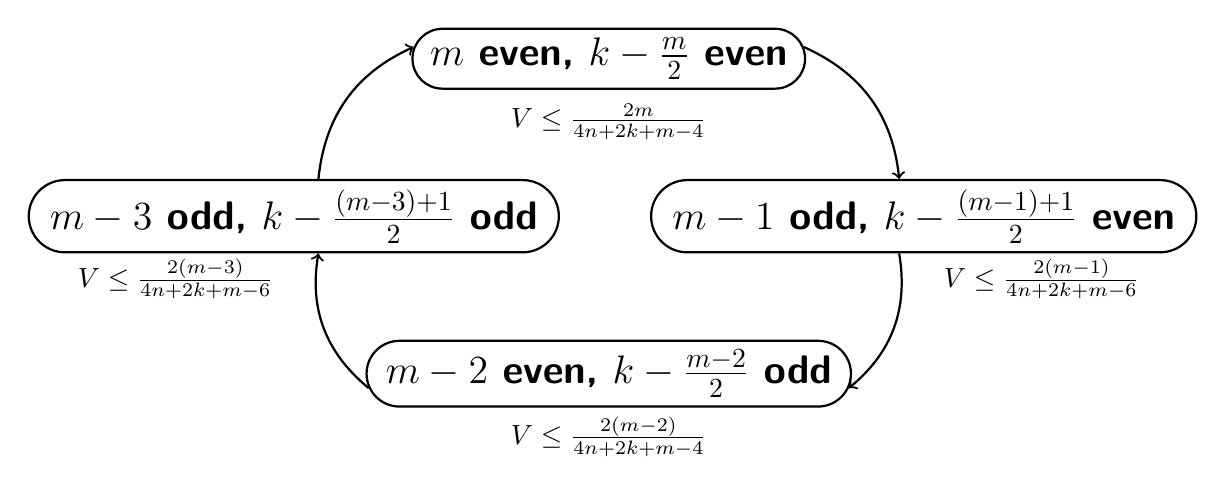
\begin{tikzpicture}[-,auto,node distance=1.5cm,
                    thick,main node/.style={rounded rectangle,fill=white,draw,font=\sffamily\Large\bfseries}]
                 
 \node[main node] (1) at (0,0) {$m$ even, $k-\frac{m}{2}$ even};
 
 \node (value1) at (0,-0.8) {$V \leq \frac{2m}{4n+2k+m-4}$}; 
 
 \node[main node] (2) at (4,-2) {$m-1$ odd, $k-\frac{(m-1)+1}{2}$ even};
 
 \node (value2) at (5.5,-2.8) {$V \leq \frac{2(m-1)}{4n+2k+m-6}$};
 
 \node[main node] (3) at (0,-4) {$m-2$ even, $k-\frac{m-2}{2}$ odd};
 
 \node (value2) at (0,-4.8) {$V \leq \frac{2(m-2)}{4n+2k+m-4}$}; 
 
 \node[main node] (4) at (-4,-2) {$m-3$ odd, $k-\frac{(m-3)+1}{2}$ odd};
 
 \node (value2) at (-5.5,-2.8) {$V \leq \frac{2(m-3)}{4n+2k+m-6}$}; 
 
 
 
  \path[->,bend left,every node/.style={font=\sffamily}]
    (1) edge (2)
    (2) edge (3)
    (3) edge (4)
    (4) edge (1);
                    
\end{tikzpicture}                    
\end{center}
\caption{Cycle of $m$ decreasing}
\end{myfigure}

The method seems to give us a pattern for the denominator which is $4$ periodic but inside the period alternates between 2 values (and does `better than expected' when $m$ is even).

\begin{myfigure}
\begin{center}
% Created by tikzDevice version 0.10.1 on 2017-11-28 18:58:33
% !TEX encoding = UTF-8 Unicode
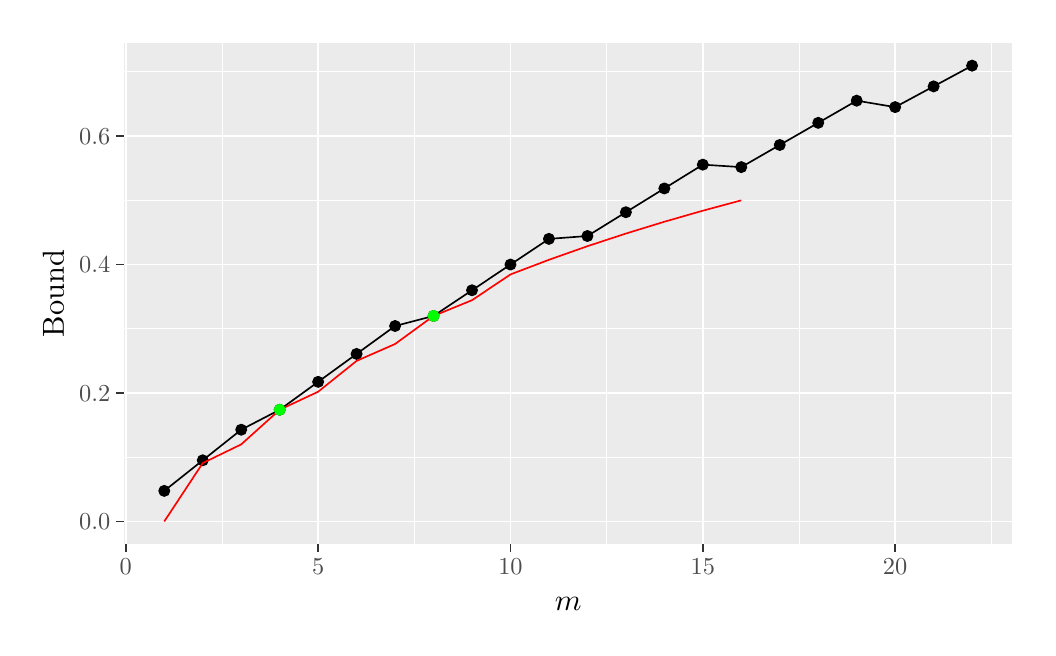
\begin{tikzpicture}[x=1pt,y=1pt]
\definecolor{fillColor}{RGB}{255,255,255}
\path[use as bounding box,fill=fillColor,fill opacity=0.00] (0,0) rectangle (361.35,216.81);
\begin{scope}
\path[clip] (  0.00,  0.00) rectangle (361.35,216.81);
\definecolor{drawColor}{RGB}{255,255,255}
\definecolor{fillColor}{RGB}{255,255,255}

\path[draw=drawColor,line width= 0.6pt,line join=round,line cap=round,fill=fillColor] (  0.00,  0.00) rectangle (361.35,216.81);
\end{scope}
\begin{scope}
\path[clip] ( 34.77, 30.14) rectangle (355.85,211.31);
\definecolor{fillColor}{gray}{0.92}

\path[fill=fillColor] ( 34.77, 30.14) rectangle (355.85,211.31);
\definecolor{drawColor}{RGB}{255,255,255}

\path[draw=drawColor,line width= 0.3pt,line join=round] ( 34.77, 61.58) --
	(355.85, 61.58);

\path[draw=drawColor,line width= 0.3pt,line join=round] ( 34.77,108.00) --
	(355.85,108.00);

\path[draw=drawColor,line width= 0.3pt,line join=round] ( 34.77,154.41) --
	(355.85,154.41);

\path[draw=drawColor,line width= 0.3pt,line join=round] ( 34.77,200.83) --
	(355.85,200.83);

\path[draw=drawColor,line width= 0.3pt,line join=round] ( 70.21, 30.14) --
	( 70.21,211.31);

\path[draw=drawColor,line width= 0.3pt,line join=round] (139.71, 30.14) --
	(139.71,211.31);

\path[draw=drawColor,line width= 0.3pt,line join=round] (209.21, 30.14) --
	(209.21,211.31);

\path[draw=drawColor,line width= 0.3pt,line join=round] (278.71, 30.14) --
	(278.71,211.31);

\path[draw=drawColor,line width= 0.3pt,line join=round] (348.21, 30.14) --
	(348.21,211.31);

\path[draw=drawColor,line width= 0.6pt,line join=round] ( 34.77, 38.38) --
	(355.85, 38.38);

\path[draw=drawColor,line width= 0.6pt,line join=round] ( 34.77, 84.79) --
	(355.85, 84.79);

\path[draw=drawColor,line width= 0.6pt,line join=round] ( 34.77,131.21) --
	(355.85,131.21);

\path[draw=drawColor,line width= 0.6pt,line join=round] ( 34.77,177.62) --
	(355.85,177.62);

\path[draw=drawColor,line width= 0.6pt,line join=round] ( 35.46, 30.14) --
	( 35.46,211.31);

\path[draw=drawColor,line width= 0.6pt,line join=round] (104.96, 30.14) --
	(104.96,211.31);

\path[draw=drawColor,line width= 0.6pt,line join=round] (174.46, 30.14) --
	(174.46,211.31);

\path[draw=drawColor,line width= 0.6pt,line join=round] (243.96, 30.14) --
	(243.96,211.31);

\path[draw=drawColor,line width= 0.6pt,line join=round] (313.46, 30.14) --
	(313.46,211.31);
\definecolor{drawColor}{RGB}{0,0,0}
\definecolor{fillColor}{RGB}{0,0,0}

\path[draw=drawColor,line width= 0.4pt,line join=round,line cap=round,fill=fillColor] ( 49.36, 49.43) circle (  1.96);

\path[draw=drawColor,line width= 0.4pt,line join=round,line cap=round,fill=fillColor] ( 63.26, 60.48) circle (  1.96);

\path[draw=drawColor,line width= 0.4pt,line join=round,line cap=round,fill=fillColor] ( 77.16, 71.53) circle (  1.96);

\path[draw=drawColor,line width= 0.4pt,line join=round,line cap=round,fill=fillColor] ( 91.06, 78.74) circle (  1.96);

\path[draw=drawColor,line width= 0.4pt,line join=round,line cap=round,fill=fillColor] (104.96, 88.83) circle (  1.96);

\path[draw=drawColor,line width= 0.4pt,line join=round,line cap=round,fill=fillColor] (118.86, 98.92) circle (  1.96);

\path[draw=drawColor,line width= 0.4pt,line join=round,line cap=round,fill=fillColor] (132.76,109.01) circle (  1.96);

\path[draw=drawColor,line width= 0.4pt,line join=round,line cap=round,fill=fillColor] (146.66,112.64) circle (  1.96);

\path[draw=drawColor,line width= 0.4pt,line join=round,line cap=round,fill=fillColor] (160.56,121.92) circle (  1.96);

\path[draw=drawColor,line width= 0.4pt,line join=round,line cap=round,fill=fillColor] (174.46,131.21) circle (  1.96);

\path[draw=drawColor,line width= 0.4pt,line join=round,line cap=round,fill=fillColor] (188.36,140.49) circle (  1.96);

\path[draw=drawColor,line width= 0.4pt,line join=round,line cap=round,fill=fillColor] (202.26,141.52) circle (  1.96);

\path[draw=drawColor,line width= 0.4pt,line join=round,line cap=round,fill=fillColor] (216.16,150.12) circle (  1.96);

\path[draw=drawColor,line width= 0.4pt,line join=round,line cap=round,fill=fillColor] (230.06,158.71) circle (  1.96);

\path[draw=drawColor,line width= 0.4pt,line join=round,line cap=round,fill=fillColor] (243.96,167.31) circle (  1.96);

\path[draw=drawColor,line width= 0.4pt,line join=round,line cap=round,fill=fillColor] (257.86,166.42) circle (  1.96);

\path[draw=drawColor,line width= 0.4pt,line join=round,line cap=round,fill=fillColor] (271.76,174.42) circle (  1.96);

\path[draw=drawColor,line width= 0.4pt,line join=round,line cap=round,fill=fillColor] (285.66,182.42) circle (  1.96);

\path[draw=drawColor,line width= 0.4pt,line join=round,line cap=round,fill=fillColor] (299.56,190.43) circle (  1.96);

\path[draw=drawColor,line width= 0.4pt,line join=round,line cap=round,fill=fillColor] (313.46,188.10) circle (  1.96);

\path[draw=drawColor,line width= 0.4pt,line join=round,line cap=round,fill=fillColor] (327.36,195.59) circle (  1.96);

\path[draw=drawColor,line width= 0.4pt,line join=round,line cap=round,fill=fillColor] (341.26,203.08) circle (  1.96);

\path[draw=drawColor,line width= 0.6pt,line join=round] ( 49.36, 49.43) --
	( 63.26, 60.48) --
	( 77.16, 71.53) --
	( 91.06, 78.74) --
	(104.96, 88.83) --
	(118.86, 98.92) --
	(132.76,109.01) --
	(146.66,112.64) --
	(160.56,121.92) --
	(174.46,131.21) --
	(188.36,140.49) --
	(202.26,141.52) --
	(216.16,150.12) --
	(230.06,158.71) --
	(243.96,167.31) --
	(257.86,166.42) --
	(271.76,174.42) --
	(285.66,182.42) --
	(299.56,190.43) --
	(313.46,188.10) --
	(327.36,195.59) --
	(341.26,203.08);
\definecolor{drawColor}{RGB}{255,0,0}

\path[draw=drawColor,line width= 0.6pt,line join=round] ( 49.36, 38.38) --
	( 63.26, 59.47) --
	( 77.16, 66.23) --
	( 91.06, 78.74) --
	(104.96, 85.26) --
	(118.86, 96.40) --
	(132.76,102.50) --
	(146.66,112.64) --
	(160.56,118.33) --
	(174.46,127.64) --
	(188.36,132.93) --
	(202.26,137.84) --
	(216.16,142.41) --
	(230.06,146.68) --
	(243.96,150.67) --
	(257.86,154.41);
\definecolor{drawColor}{RGB}{0,255,0}
\definecolor{fillColor}{RGB}{0,255,0}

\path[draw=drawColor,line width= 0.4pt,line join=round,line cap=round,fill=fillColor] ( 91.06, 78.74) circle (  1.96);

\path[draw=drawColor,line width= 0.4pt,line join=round,line cap=round,fill=fillColor] (146.66,112.64) circle (  1.96);
\end{scope}
\begin{scope}
\path[clip] (  0.00,  0.00) rectangle (361.35,216.81);
\definecolor{drawColor}{gray}{0.30}

\node[text=drawColor,anchor=base east,inner sep=0pt, outer sep=0pt, scale=  0.88] at ( 29.82, 35.35) {0.0};

\node[text=drawColor,anchor=base east,inner sep=0pt, outer sep=0pt, scale=  0.88] at ( 29.82, 81.76) {0.2};

\node[text=drawColor,anchor=base east,inner sep=0pt, outer sep=0pt, scale=  0.88] at ( 29.82,128.18) {0.4};

\node[text=drawColor,anchor=base east,inner sep=0pt, outer sep=0pt, scale=  0.88] at ( 29.82,174.59) {0.6};
\end{scope}
\begin{scope}
\path[clip] (  0.00,  0.00) rectangle (361.35,216.81);
\definecolor{drawColor}{gray}{0.20}

\path[draw=drawColor,line width= 0.6pt,line join=round] ( 32.02, 38.38) --
	( 34.77, 38.38);

\path[draw=drawColor,line width= 0.6pt,line join=round] ( 32.02, 84.79) --
	( 34.77, 84.79);

\path[draw=drawColor,line width= 0.6pt,line join=round] ( 32.02,131.21) --
	( 34.77,131.21);

\path[draw=drawColor,line width= 0.6pt,line join=round] ( 32.02,177.62) --
	( 34.77,177.62);
\end{scope}
\begin{scope}
\path[clip] (  0.00,  0.00) rectangle (361.35,216.81);
\definecolor{drawColor}{gray}{0.20}

\path[draw=drawColor,line width= 0.6pt,line join=round] ( 35.46, 27.39) --
	( 35.46, 30.14);

\path[draw=drawColor,line width= 0.6pt,line join=round] (104.96, 27.39) --
	(104.96, 30.14);

\path[draw=drawColor,line width= 0.6pt,line join=round] (174.46, 27.39) --
	(174.46, 30.14);

\path[draw=drawColor,line width= 0.6pt,line join=round] (243.96, 27.39) --
	(243.96, 30.14);

\path[draw=drawColor,line width= 0.6pt,line join=round] (313.46, 27.39) --
	(313.46, 30.14);
\end{scope}
\begin{scope}
\path[clip] (  0.00,  0.00) rectangle (361.35,216.81);
\definecolor{drawColor}{gray}{0.30}

\node[text=drawColor,anchor=base,inner sep=0pt, outer sep=0pt, scale=  0.88] at ( 35.46, 19.13) {0};

\node[text=drawColor,anchor=base,inner sep=0pt, outer sep=0pt, scale=  0.88] at (104.96, 19.13) {5};

\node[text=drawColor,anchor=base,inner sep=0pt, outer sep=0pt, scale=  0.88] at (174.46, 19.13) {10};

\node[text=drawColor,anchor=base,inner sep=0pt, outer sep=0pt, scale=  0.88] at (243.96, 19.13) {15};

\node[text=drawColor,anchor=base,inner sep=0pt, outer sep=0pt, scale=  0.88] at (313.46, 19.13) {20};
\end{scope}
\begin{scope}
\path[clip] (  0.00,  0.00) rectangle (361.35,216.81);
\definecolor{drawColor}{RGB}{0,0,0}

\node[text=drawColor,anchor=base,inner sep=0pt, outer sep=0pt, scale=  1.10] at (195.31,  6.06) {$m$};
\end{scope}
\begin{scope}
\path[clip] (  0.00,  0.00) rectangle (361.35,216.81);
\definecolor{drawColor}{RGB}{0,0,0}

\node[text=drawColor,rotate= 90.00,anchor=base,inner sep=0pt, outer sep=0pt, scale=  1.10] at ( 13.08,120.73) {Bound};
\end{scope}
\end{tikzpicture}

\end{center}
\caption{A plot of the UpperBound and the Combinatorial Improvement bound for $S_{6}^{10}$}
\end{myfigure}

We can notice the other even $m$ seems to be close to the Combinatorial improvement but is slightly too high, this could suggest that we can make a further improvement on the combinatorial (Though logistically this seems hard) or we can perform a better attack (This may require something like on the line). We will go to this type of analysis now


\subsection{Lower Line type attacks}
Looking at $S_{7}^{5}$
We note that by the above we know the solution for all even $m$ bar $6,10$ in the graph. We present a solution for $m=6$ in the form of a grid

\begin{myfigure}
\begin{center}
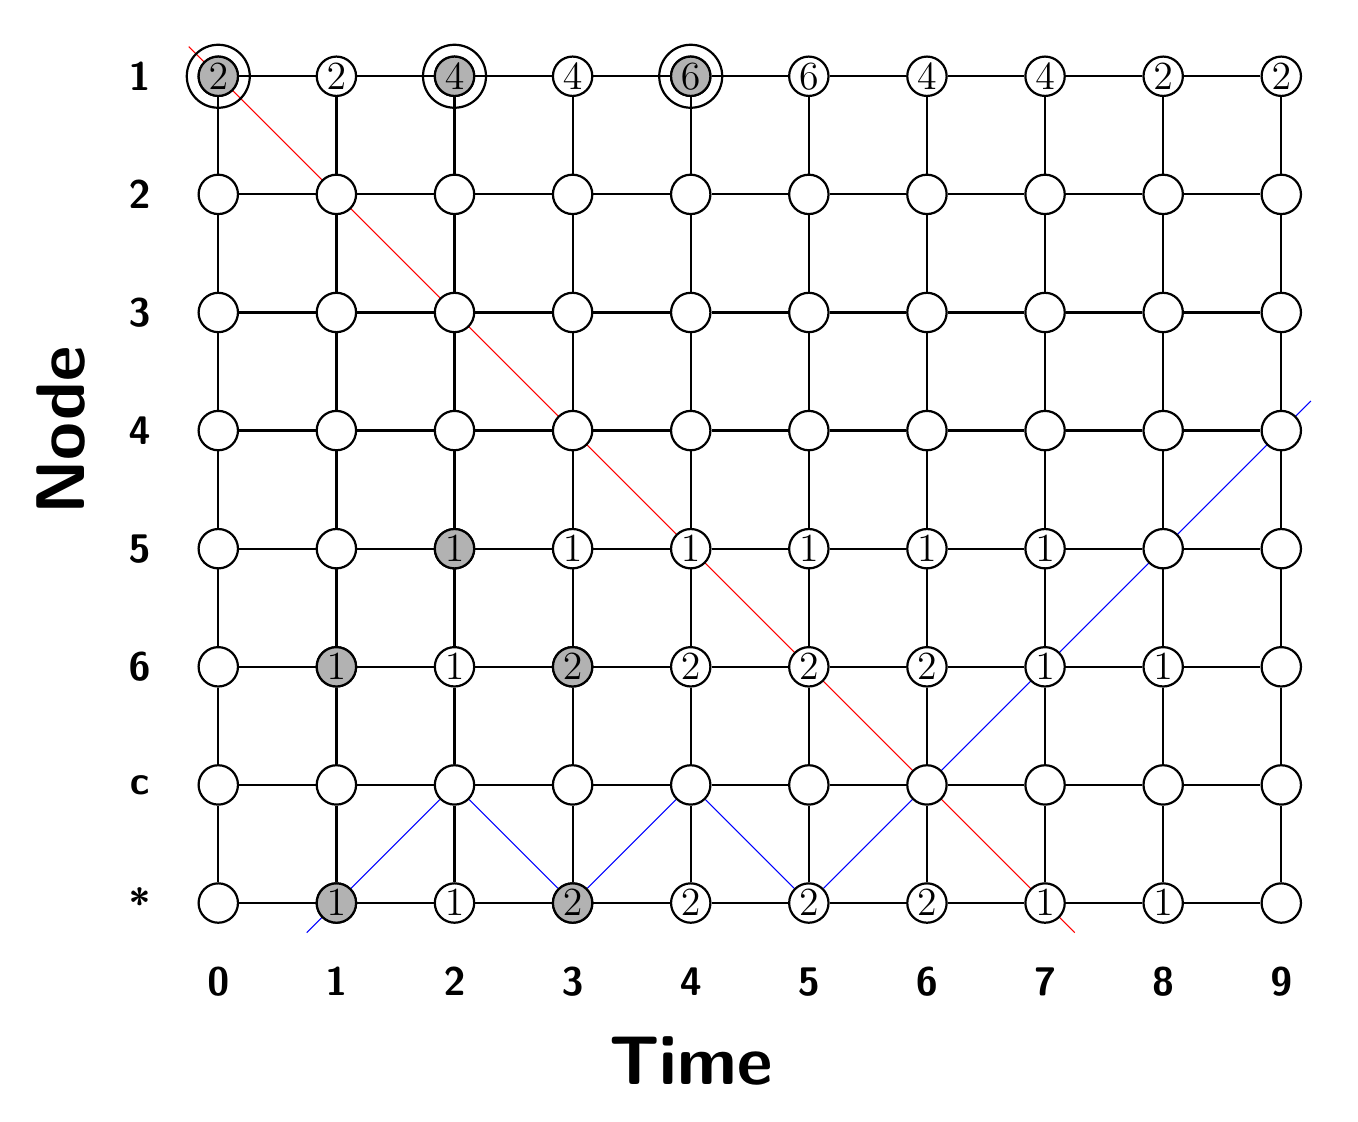
\begin{tikzpicture}[-,auto,node distance=1cm,
                    thick,main node/.style={circle,fill=white,draw,font=\sffamily\Large\bfseries,minimum size=0.5cm}]
 \foreach \x in {0,...,9}
    \foreach \y in {0,...,7} 
       {\pgfmathtruncatemacro{\label}{\x - 5 *  \y +21}
       \node [main node]  (\x\y) at (1.5*\x,1.5*\y) {};} 

  \foreach \x in {0,...,8}
   \foreach \y in {0,...,6}
    \pgfmathtruncatemacro{\za}{\y+1}
    \pgfmathtruncatemacro{\zb}{\x+1}
      \draw (\x\y)--(\x\za) (\x\y)--(\zb\y) ;
      
   \foreach \x in {0,...,8}
    \pgfmathtruncatemacro{\zb}{\x+1}
      \draw (\x7) -- (\zb7);
      
   \foreach \y in {0,...,6}
     \pgfmathtruncatemacro{\za}{\y+1} 
        \draw (9\y) -- (9\za);
        
        
%Labeling to the sides
  \foreach \y in {2,...,7}
   \pgfmathtruncatemacro{\label}{8-\y}
   \node[font=\sffamily\Large\bfseries] (Label\y) [shift={(-1,0)}] at (0\y) {\label};       
   
   \node[font=\sffamily\Large\bfseries] (Label) [shift={(-1,0)}] at (01) {c};
   \node[font=\sffamily\Large\bfseries] (Label) [shift={(-1,0)}] at (00) {*};
   
   \node[font=\sffamily\Huge\bfseries] (Axis) [shift={(-2,0)},rotate=90] at (04) {Node};

   \foreach \x in {0,...,9}
    \node[font=\sffamily\Large\bfseries] (Timelabel\x) [shift={(0,-1)}] at (\x0) {\x};
    
   \node[font=\sffamily\Huge\bfseries] (Axis) [shift={(0,-2)}] at (40) {Time};
    
    
%Adding in top attacks        
   \node[main node,fill=gray!60] (07) at (07) {};    
   \node[circle,draw,minimum size=0.8cm] (Attack1) at (07) {};
   
   \node[main node,fill=gray!60] (27) at (27) {};    
   \node[circle,draw,minimum size=0.8cm] (Attack2) at (27) {};     
   
   \node[main node,fill=gray!60] (47) at (47) {};    
   \node[circle,draw,minimum size=0.8cm] (Attack3) at (47) {};
   
   %Attack numbers
    \node[font=\sffamily\Large\bfseries] (AttackNumber1)  at (07) {$2$};
    \node[font=\sffamily\Large\bfseries] (AttackNumber1)  at (17) {$2$}; 
    \node[font=\sffamily\Large\bfseries] (AttackNumber1)  at (27) {$4$}; 
    \node[font=\sffamily\Large\bfseries] (AttackNumber1)  at (37) {$4$}; 
    \node[font=\sffamily\Large\bfseries] (AttackNumber1)  at (47) {$6$}; 
    \node[font=\sffamily\Large\bfseries] (AttackNumber1)  at (57) {$6$}; 
    \node[font=\sffamily\Large\bfseries] (AttackNumber1)  at (67) {$4$}; 
    \node[font=\sffamily\Large\bfseries] (AttackNumber1)  at (77) {$4$}; 
    \node[font=\sffamily\Large\bfseries] (AttackNumber1)  at (87) {$2$}; 
    \node[font=\sffamily\Large\bfseries] (AttackNumber1)  at (97) {$2$}; 
          
   
%Adding in middle attacks
  \node[main node,fill=gray!60] (23) at (23) {};
  \node[main node,fill=gray!60] (12) at (12) {};
  \node[main node,fill=gray!60] (32) at (32) {};
     
    %Attack numbers
    \node[font=\sffamily\Large\bfseries] (AttackNumber1)  at (23) {$1$};
    \node[font=\sffamily\Large\bfseries] (AttackNumber1)  at (33) {$1$}; 
    \node[font=\sffamily\Large\bfseries] (AttackNumber1)  at (43) {$1$}; 
    \node[font=\sffamily\Large\bfseries] (AttackNumber1)  at (53) {$1$}; 
    \node[font=\sffamily\Large\bfseries] (AttackNumber1)  at (63) {$1$}; 
    \node[font=\sffamily\Large\bfseries] (AttackNumber1)  at (73) {$1$};
     
    \node[font=\sffamily\Large\bfseries] (AttackNumber1)  at (12) {$1$}; 
    \node[font=\sffamily\Large\bfseries] (AttackNumber1)  at (22) {$1$}; 
    \node[font=\sffamily\Large\bfseries] (AttackNumber1)  at (32) {$2$}; 
    \node[font=\sffamily\Large\bfseries] (AttackNumber1)  at (42) {$2$}; 
    \node[font=\sffamily\Large\bfseries] (AttackNumber1)  at (52) {$2$}; 
    \node[font=\sffamily\Large\bfseries] (AttackNumber1)  at (62) {$2$}; 
    \node[font=\sffamily\Large\bfseries] (AttackNumber1)  at (72) {$1$}; 
    \node[font=\sffamily\Large\bfseries] (AttackNumber1)  at (82) {$1$};   
%Adding bottom attacks

 \node[main node,fill=gray!60] (10) at (10) {};
 \node[main node,fill=gray!60] (30) at (30) {};
 
    %Attack numbers
    \node[font=\sffamily\Large\bfseries] (AttackNumber1)  at (10) {$1$}; 
    \node[font=\sffamily\Large\bfseries] (AttackNumber1)  at (20) {$1$}; 
    \node[font=\sffamily\Large\bfseries] (AttackNumber1)  at (30) {$2$}; 
    \node[font=\sffamily\Large\bfseries] (AttackNumber1)  at (40) {$2$}; 
    \node[font=\sffamily\Large\bfseries] (AttackNumber1)  at (50) {$2$}; 
    \node[font=\sffamily\Large\bfseries] (AttackNumber1)  at (60) {$2$}; 
    \node[font=\sffamily\Large\bfseries] (AttackNumber1)  at (70) {$1$}; 
    \node[font=\sffamily\Large\bfseries] (AttackNumber1)  at (80) {$1$};        
        
                 
%Some example lines drawn
\begin{scope}[on background layer]
\node (a)[shift={(-0.5,0.5)}] at (07) {};
\node (b)[shift={(0.5,-0.5)}] at (70) {};
\draw[color=red] (a) -- (b);

\node (c)[shift={(-0.5,-0.5)}] at (10) {};
\node (d)[shift={(0.5,0.5)}] at (94) {};
\draw[color=blue] (c) -- (21) (21) -- (30) (30)--(41) (41) -- (50) (50)--(d);

\end{scope}

                   
\end{tikzpicture}
\end{center}
\caption{Grid solution of $m=6$ on $S_{7}^{5}$ with two example paths}
\end{myfigure}

\begin{note}
We note that a reflection is possible at the end $*$ and we still gain the number again (unlike usual)
\end{note}

This allows us to get $V(S_{7}^{5},m=6)=\frac{6}{21}$ (by combinatorial and this attack pattern).

We could try to guess the solution for $m=10$ in $S_{7}^{5}$ using the same idea ? let's investigate, if it holds we wish to get the value of $V(S_{7}^{5},m=10)=\frac{10}{23}$ to match with the combinatorial improvement, however here $m=2k$ ,so the solution is known to give $V(S_{7}^{5},m=10)=\frac{10}{22}$ by decomposition into $S_{6}$ and $L_{6}$ and $10$ attacks at node $1$ and $12$ attacks at $*$ nodes (spaced accordingly).

So perhaps we need to consider a bigger example, let us look at $S_{7}^{9}$ and again we look at $m=6$ first then we would want to get $V=\frac{6}{25}$, this would mean adapting our current attack to place $4$ more attacks, well this is infact due to having an additonal $4$ nodes along the line we guess we shouldn't have too much of an issue.

\begin{myfigure}
\centering
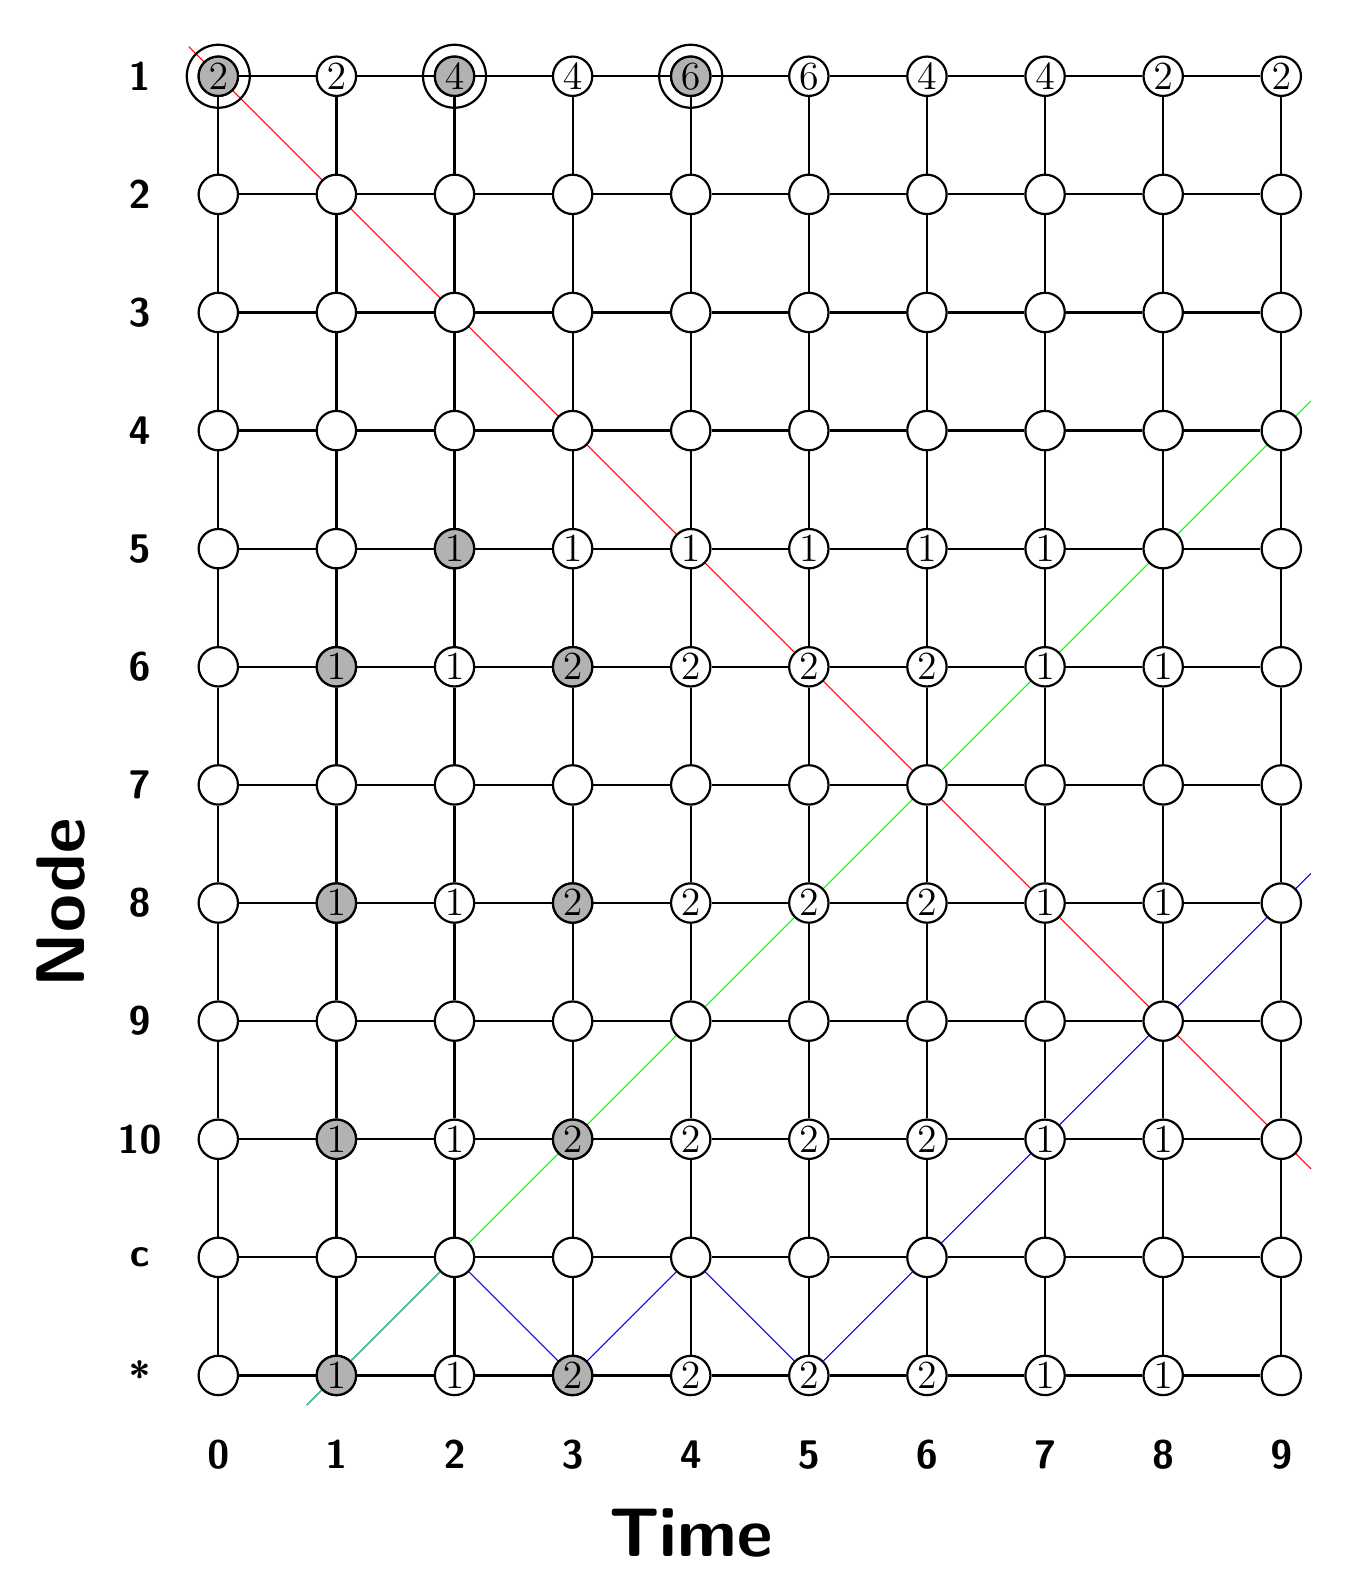
\begin{tikzpicture}[-,auto,node distance=1cm,
                    thick,main node/.style={circle,fill=white,draw,font=\sffamily\Large\bfseries,minimum size=0.5cm}]
 \foreach \x in {0,...,9}
    \foreach \y in {0,...,11} 
       {\pgfmathtruncatemacro{\label}{\x - 5 *  \y +21}
       \node [main node]  (\x\y) at (1.5*\x,1.5*\y) {};} 

  \foreach \x in {0,...,8}
   \foreach \y in {0,...,10}
    \pgfmathtruncatemacro{\za}{\y+1}
    \pgfmathtruncatemacro{\zb}{\x+1}
      \draw (\x\y)--(\x\za) (\x\y)--(\zb\y) ;
      
   \foreach \x in {0,...,8}
    \pgfmathtruncatemacro{\zb}{\x+1}
      \draw (\x11) -- (\zb11);
      
   \foreach \y in {0,...,10}
     \pgfmathtruncatemacro{\za}{\y+1} 
        \draw (9\y) -- (9\za);
        
        
%Labeling to the sides
  \foreach \y in {2,...,11}
   \pgfmathtruncatemacro{\label}{12-\y}
   \node[font=\sffamily\Large\bfseries] (Label\y) [shift={(-1,0)}] at (0\y) {\label};       
   
   \node[font=\sffamily\Large\bfseries] (Label) [shift={(-1,0)}] at (01) {c};
   \node[font=\sffamily\Large\bfseries] (Label) [shift={(-1,0)}] at (00) {*};
   
   \node[font=\sffamily\Huge\bfseries] (Axis) [shift={(-2,0)},rotate=90] at (04) {Node};

   \foreach \x in {0,...,9}
    \node[font=\sffamily\Large\bfseries] (Timelabel\x) [shift={(0,-1)}] at (\x0) {\x};
    
   \node[font=\sffamily\Huge\bfseries] (Axis) [shift={(0,-2)}] at (40) {Time};
    
    
%Adding in top attacks        
   \node[main node,fill=gray!60] (011) at (011) {};    
   \node[circle,draw,minimum size=0.8cm] (Attack1) at (011) {};
   
   \node[main node,fill=gray!60] (211) at (211) {};    
   \node[circle,draw,minimum size=0.8cm] (Attack2) at (211) {};     
   
   \node[main node,fill=gray!60] (411) at (411) {};    
   \node[circle,draw,minimum size=0.8cm] (Attack3) at (411) {};
   
   %Attack numbers
    \node[font=\sffamily\Large\bfseries] (AttackNumber1)  at (011) {$2$};
    \node[font=\sffamily\Large\bfseries] (AttackNumber1)  at (111) {$2$}; 
    \node[font=\sffamily\Large\bfseries] (AttackNumber1)  at (211) {$4$}; 
    \node[font=\sffamily\Large\bfseries] (AttackNumber1)  at (311) {$4$}; 
    \node[font=\sffamily\Large\bfseries] (AttackNumber1)  at (411) {$6$}; 
    \node[font=\sffamily\Large\bfseries] (AttackNumber1)  at (511) {$6$}; 
    \node[font=\sffamily\Large\bfseries] (AttackNumber1)  at (611) {$4$}; 
    \node[font=\sffamily\Large\bfseries] (AttackNumber1)  at (711) {$4$}; 
    \node[font=\sffamily\Large\bfseries] (AttackNumber1)  at (811) {$2$}; 
    \node[font=\sffamily\Large\bfseries] (AttackNumber1)  at (911) {$2$}; 
          
   
%Adding in middle attacks



  \node[main node,fill=gray!60] (27) at (27) {};
  
  \node[main node,fill=gray!60] (16) at (16) {};
  \node[main node,fill=gray!60] (36) at (36) {};
  
  \node[main node,fill=gray!60] (14) at (14) {};
  \node[main node,fill=gray!60] (34) at (34) {};
  
  \node[main node,fill=gray!60] (12) at (12) {};
  \node[main node,fill=gray!60] (32) at (32) {};
     
    %Attack numbers
    
    \node[font=\sffamily\Large\bfseries] (AttackNumber1)  at (27) {$1$};
    \node[font=\sffamily\Large\bfseries] (AttackNumber1)  at (37) {$1$}; 
    \node[font=\sffamily\Large\bfseries] (AttackNumber1)  at (47) {$1$}; 
    \node[font=\sffamily\Large\bfseries] (AttackNumber1)  at (57) {$1$}; 
    \node[font=\sffamily\Large\bfseries] (AttackNumber1)  at (67) {$1$}; 
    \node[font=\sffamily\Large\bfseries] (AttackNumber1)  at (77) {$1$};
     
    \node[font=\sffamily\Large\bfseries] (AttackNumber1)  at (12) {$1$}; 
    \node[font=\sffamily\Large\bfseries] (AttackNumber1)  at (22) {$1$}; 
    \node[font=\sffamily\Large\bfseries] (AttackNumber1)  at (32) {$2$}; 
    \node[font=\sffamily\Large\bfseries] (AttackNumber1)  at (42) {$2$}; 
    \node[font=\sffamily\Large\bfseries] (AttackNumber1)  at (52) {$2$}; 
    \node[font=\sffamily\Large\bfseries] (AttackNumber1)  at (62) {$2$}; 
    \node[font=\sffamily\Large\bfseries] (AttackNumber1)  at (72) {$1$}; 
    \node[font=\sffamily\Large\bfseries] (AttackNumber1)  at (82) {$1$};
    
    \node[font=\sffamily\Large\bfseries] (AttackNumber1)  at (14) {$1$}; 
    \node[font=\sffamily\Large\bfseries] (AttackNumber1)  at (24) {$1$}; 
    \node[font=\sffamily\Large\bfseries] (AttackNumber1)  at (34) {$2$}; 
    \node[font=\sffamily\Large\bfseries] (AttackNumber1)  at (44) {$2$}; 
    \node[font=\sffamily\Large\bfseries] (AttackNumber1)  at (54) {$2$}; 
    \node[font=\sffamily\Large\bfseries] (AttackNumber1)  at (64) {$2$}; 
    \node[font=\sffamily\Large\bfseries] (AttackNumber1)  at (74) {$1$}; 
    \node[font=\sffamily\Large\bfseries] (AttackNumber1)  at (84) {$1$};
    
    \node[font=\sffamily\Large\bfseries] (AttackNumber1)  at (16) {$1$}; 
    \node[font=\sffamily\Large\bfseries] (AttackNumber1)  at (26) {$1$}; 
    \node[font=\sffamily\Large\bfseries] (AttackNumber1)  at (36) {$2$}; 
    \node[font=\sffamily\Large\bfseries] (AttackNumber1)  at (46) {$2$}; 
    \node[font=\sffamily\Large\bfseries] (AttackNumber1)  at (56) {$2$}; 
    \node[font=\sffamily\Large\bfseries] (AttackNumber1)  at (66) {$2$}; 
    \node[font=\sffamily\Large\bfseries] (AttackNumber1)  at (76) {$1$}; 
    \node[font=\sffamily\Large\bfseries] (AttackNumber1)  at (86) {$1$};
    
       
%Adding bottom attacks

 \node[main node,fill=gray!60] (10) at (10) {};
 \node[main node,fill=gray!60] (30) at (30) {};
 
    %Attack numbers
    \node[font=\sffamily\Large\bfseries] (AttackNumber1)  at (10) {$1$}; 
    \node[font=\sffamily\Large\bfseries] (AttackNumber1)  at (20) {$1$}; 
    \node[font=\sffamily\Large\bfseries] (AttackNumber1)  at (30) {$2$}; 
    \node[font=\sffamily\Large\bfseries] (AttackNumber1)  at (40) {$2$}; 
    \node[font=\sffamily\Large\bfseries] (AttackNumber1)  at (50) {$2$}; 
    \node[font=\sffamily\Large\bfseries] (AttackNumber1)  at (60) {$2$}; 
    \node[font=\sffamily\Large\bfseries] (AttackNumber1)  at (70) {$1$}; 
    \node[font=\sffamily\Large\bfseries] (AttackNumber1)  at (80) {$1$};        
        
                 
%Some example lines drawn
\begin{scope}[on background layer]
\node (a)[shift={(-0.5,0.5)}] at (011) {};
\node (b)[shift={(0.5,-0.5)}] at (92) {};
\draw[color=red] (a) -- (b);

\node (c)[shift={(-0.5,-0.5)}] at (10) {};
\node (d)[shift={(0.5,0.5)}] at (94) {};
\draw[color=blue] (c) -- (21) (21) -- (30) (30)--(41) (41) -- (50) (50)--(d);

\node (e) [shift={(0.5,0.5)}] at(98) {};
\draw[color=green] (c) -- (e);

\end{scope}

                   
\end{tikzpicture}
\caption{Grid solution of $m=6$ on $S_{7}^{9}$ with three example paths}
\end{myfigure}

We have the solution $V(S_{7}^{9},m=6)=\frac{6}{25}$. Now we want to see if this logic applies to $m=10$, by the combinatorial bound we expect that $V=\frac{10}{27}$ that is to place $2$ more attacks.

\begin{myfigure}
\resizebox{1\linewidth}{!}{
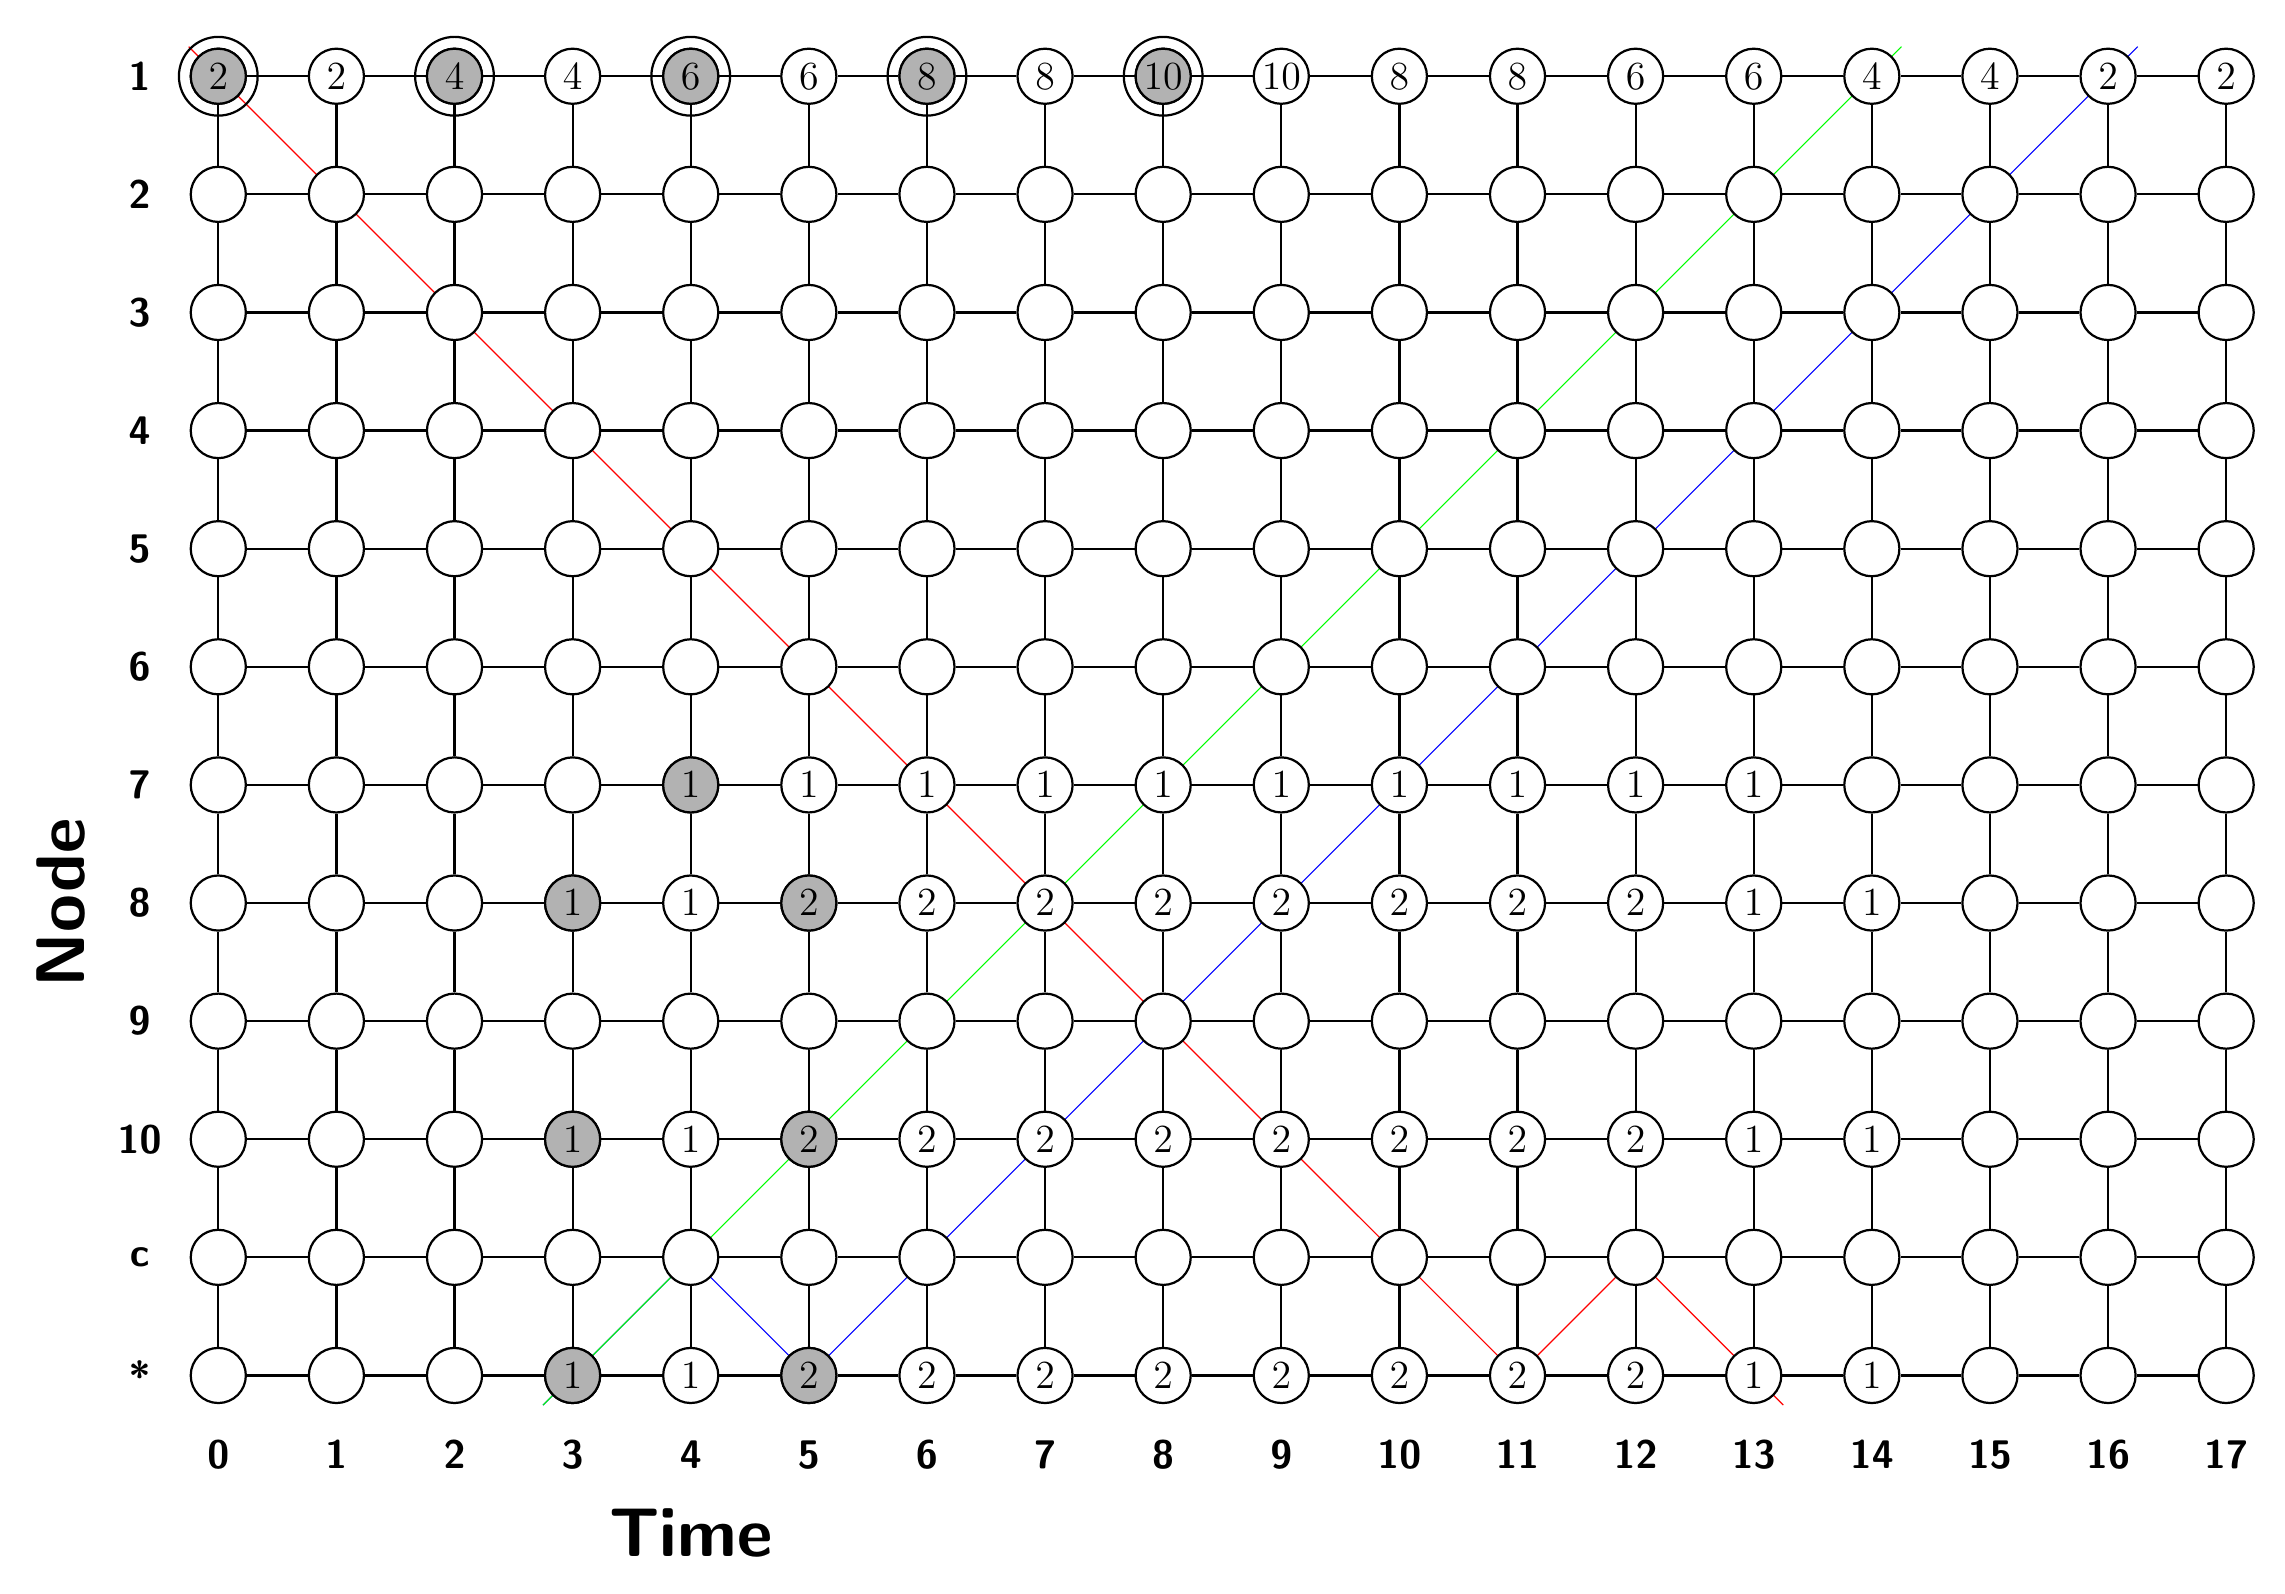
\begin{tikzpicture}[-,auto,node distance=1cm,
                    thick,main node/.style={circle,fill=white,draw,font=\sffamily\Large\bfseries,minimum size=0.7cm}]
 \foreach \x in {0,...,17}
    \foreach \y in {0,...,11} 
       {\pgfmathtruncatemacro{\label}{\x - 5 *  \y +21}
       \node [main node]  (\x0\y) at (1.5*\x,1.5*\y) {};} 

  \foreach \x in {0,...,16}
   \foreach \y in {0,...,10}
    \pgfmathtruncatemacro{\za}{\y+1}
    \pgfmathtruncatemacro{\zb}{\x+1}
      \draw (\x0\y)--(\x0\za) (\x0\y)--(\zb0\y) ;
      
   \foreach \x in {0,...,16}
    \pgfmathtruncatemacro{\zb}{\x+1}
      \draw (\x011) -- (\zb011);
      
   \foreach \y in {0,...,10}
     \pgfmathtruncatemacro{\za}{\y+1} 
        \draw (170\y) -- (170\za);
        
        
%Labeling to the sides
  \foreach \y in {2,...,11}
   \pgfmathtruncatemacro{\label}{12-\y}
   \node[font=\sffamily\Large\bfseries] (Label\y) [shift={(-1,0)}] at (00\y) {\label};       
   
   \node[font=\sffamily\Large\bfseries] (Label) [shift={(-1,0)}] at (001) {c};
   \node[font=\sffamily\Large\bfseries] (Label) [shift={(-1,0)}] at (000) {*};
   
   \node[font=\sffamily\Huge\bfseries] (Axis) [shift={(-2,0)},rotate=90] at (004) {Node};

   \foreach \x in {0,...,17}
    \node[font=\sffamily\Large\bfseries] (Timelabel\x) [shift={(0,-1)}] at (\x00) {\x};
    
   \node[font=\sffamily\Huge\bfseries] (Axis) [shift={(0,-2)}] at (400) {Time};
    
    
%Adding in top attacks        
   \node[main node,fill=gray!60] (0011) at (0011) {};    
   \node[circle,draw,minimum size=1cm] (Attack1) at (0011) {};
   
   \node[main node,fill=gray!60] (2011) at (2011) {};    
   \node[circle,draw,minimum size=1cm] (Attack2) at (2011) {};     
   
   \node[main node,fill=gray!60] (4011) at (4011) {};    
   \node[circle,draw,minimum size=1cm] (Attack3) at (4011) {};

   \node[main node,fill=gray!60] (6011) at (6011) {};    
   \node[circle,draw,minimum size=1cm] (Attack3) at (6011) {};

   \node[main node,fill=gray!60] (8011) at (8011) {};    
   \node[circle,draw,minimum size=1cm] (Attack3) at (8011) {};      
   
   %Attack numbers
    \node[font=\sffamily\Large\bfseries] (AttackNumber1)  at (0011) {$2$};
    \node[font=\sffamily\Large\bfseries] (AttackNumber1)  at (1011) {$2$}; 
    \node[font=\sffamily\Large\bfseries] (AttackNumber1)  at (2011) {$4$}; 
    \node[font=\sffamily\Large\bfseries] (AttackNumber1)  at (3011) {$4$}; 
    \node[font=\sffamily\Large\bfseries] (AttackNumber1)  at (4011) {$6$}; 
    \node[font=\sffamily\Large\bfseries] (AttackNumber1)  at (5011) {$6$}; 
    \node[font=\sffamily\Large\bfseries] (AttackNumber1)  at (6011) {$8$}; 
    \node[font=\sffamily\Large\bfseries] (AttackNumber1)  at (7011) {$8$}; 
    \node[font=\sffamily\Large\bfseries] (AttackNumber1)  at (8011) {$10$}; 
    \node[font=\sffamily\Large\bfseries] (AttackNumber1)  at (9011) {$10$};
    \node[font=\sffamily\Large\bfseries] (AttackNumber1)  at (10011) {$8$}; 
    \node[font=\sffamily\Large\bfseries] (AttackNumber1)  at (11011) {$8$}; 
    \node[font=\sffamily\Large\bfseries] (AttackNumber1)  at (12011) {$6$}; 
    \node[font=\sffamily\Large\bfseries] (AttackNumber1)  at (13011) {$6$}; 
    \node[font=\sffamily\Large\bfseries] (AttackNumber1)  at (14011) {$4$}; 
    \node[font=\sffamily\Large\bfseries] (AttackNumber1)  at (15011) {$4$}; 
    \node[font=\sffamily\Large\bfseries] (AttackNumber1)  at (16011) {$2$}; 
    \node[font=\sffamily\Large\bfseries] (AttackNumber1)  at (17011) {$2$};     
          
   
%Adding in middle attacks



  \node[main node,fill=gray!60] (405) at (405) {};

  \node[main node,fill=gray!60] (304) at (304) {};
  \node[main node,fill=gray!60] (504) at (504) {};
  
  \node[main node,fill=gray!60] (302) at (302) {};
  \node[main node,fill=gray!60] (502) at (502) {};
     
    %Attack numbers
    
    \node[font=\sffamily\Large\bfseries] (AttackNumber1)  at (405) {$1$};
    \node[font=\sffamily\Large\bfseries] (AttackNumber1)  at (505) {$1$}; 
    \node[font=\sffamily\Large\bfseries] (AttackNumber1)  at (605) {$1$}; 
    \node[font=\sffamily\Large\bfseries] (AttackNumber1)  at (705) {$1$}; 
    \node[font=\sffamily\Large\bfseries] (AttackNumber1)  at (805) {$1$}; 
    \node[font=\sffamily\Large\bfseries] (AttackNumber1)  at (905) {$1$};
    \node[font=\sffamily\Large\bfseries] (AttackNumber1)  at (1005) {$1$}; 
    \node[font=\sffamily\Large\bfseries] (AttackNumber1)  at (1105) {$1$};
    \node[font=\sffamily\Large\bfseries] (AttackNumber1)  at (1205) {$1$}; 
    \node[font=\sffamily\Large\bfseries] (AttackNumber1)  at (1305) {$1$};        

    \node[font=\sffamily\Large\bfseries] (AttackNumber1)  at (304) {$1$}; 
    \node[font=\sffamily\Large\bfseries] (AttackNumber1)  at (404) {$1$};
    \node[font=\sffamily\Large\bfseries] (AttackNumber1)  at (504) {$2$}; 
    \node[font=\sffamily\Large\bfseries] (AttackNumber1)  at (604) {$2$}; 
    \node[font=\sffamily\Large\bfseries] (AttackNumber1)  at (704) {$2$}; 
    \node[font=\sffamily\Large\bfseries] (AttackNumber1)  at (804) {$2$}; 
    \node[font=\sffamily\Large\bfseries] (AttackNumber1)  at (904) {$2$};
    \node[font=\sffamily\Large\bfseries] (AttackNumber1)  at (1004) {$2$}; 
    \node[font=\sffamily\Large\bfseries] (AttackNumber1)  at (1104) {$2$};
    \node[font=\sffamily\Large\bfseries] (AttackNumber1)  at (1204) {$2$}; 
    \node[font=\sffamily\Large\bfseries] (AttackNumber1)  at (1304) {$1$};
    \node[font=\sffamily\Large\bfseries] (AttackNumber1)  at (1404) {$1$};
    
    \node[font=\sffamily\Large\bfseries] (AttackNumber1)  at (302) {$1$}; 
    \node[font=\sffamily\Large\bfseries] (AttackNumber1)  at (402) {$1$};
    \node[font=\sffamily\Large\bfseries] (AttackNumber1)  at (502) {$2$}; 
    \node[font=\sffamily\Large\bfseries] (AttackNumber1)  at (602) {$2$}; 
    \node[font=\sffamily\Large\bfseries] (AttackNumber1)  at (702) {$2$}; 
    \node[font=\sffamily\Large\bfseries] (AttackNumber1)  at (802) {$2$}; 
    \node[font=\sffamily\Large\bfseries] (AttackNumber1)  at (902) {$2$};
    \node[font=\sffamily\Large\bfseries] (AttackNumber1)  at (1002) {$2$}; 
    \node[font=\sffamily\Large\bfseries] (AttackNumber1)  at (1102) {$2$};
    \node[font=\sffamily\Large\bfseries] (AttackNumber1)  at (1202) {$2$}; 
    \node[font=\sffamily\Large\bfseries] (AttackNumber1)  at (1302) {$1$};
    \node[font=\sffamily\Large\bfseries] (AttackNumber1)  at (1402) {$1$};    
    
       
%Adding bottom attacks

 \node[main node,fill=gray!60] (300) at (300) {};
 \node[main node,fill=gray!60] (500) at (500) {};
 
    %Attack numbers
    \node[font=\sffamily\Large\bfseries] (AttackNumber1)  at (300) {$1$}; 
    \node[font=\sffamily\Large\bfseries] (AttackNumber1)  at (400) {$1$};
    \node[font=\sffamily\Large\bfseries] (AttackNumber1)  at (500) {$2$}; 
    \node[font=\sffamily\Large\bfseries] (AttackNumber1)  at (600) {$2$}; 
    \node[font=\sffamily\Large\bfseries] (AttackNumber1)  at (700) {$2$}; 
    \node[font=\sffamily\Large\bfseries] (AttackNumber1)  at (800) {$2$}; 
    \node[font=\sffamily\Large\bfseries] (AttackNumber1)  at (900) {$2$};
    \node[font=\sffamily\Large\bfseries] (AttackNumber1)  at (1000) {$2$}; 
    \node[font=\sffamily\Large\bfseries] (AttackNumber1)  at (1100) {$2$};
    \node[font=\sffamily\Large\bfseries] (AttackNumber1)  at (1200) {$2$}; 
    \node[font=\sffamily\Large\bfseries] (AttackNumber1)  at (1300) {$1$};
    \node[font=\sffamily\Large\bfseries] (AttackNumber1)  at (1400) {$1$};      
        
                 
%Some example lines drawn
\begin{scope}[on background layer]
\node (a)[shift={(-0.5,0.5)}] at (0011) {};
\node (b)[shift={(0.5,-0.5)}] at (1300) {};
\draw[color=red] (a) -- (1100) (1100)--(1201) (1201)--(b) ;

\node (c)[shift={(-0.5,-0.5)}] at (300) {};
\node (d)[shift={(0.5,0.5)}] at (16011) {};
\draw[color=blue] (c)--(401) (401)--(500) (500)--(d);

\node (e) [shift={(0.5,0.5)}] at(14011) {};
\draw[color=green] (c) -- (e);

\end{scope}

                   
\end{tikzpicture}
}
\caption{Grid solution of $m=10$ on $S_{7}^{9}$ with three example paths}
\end{myfigure}

As expected.

Hence we need to perform a generalisation to give us the answer when $m \leq 2(n-1)$ for all even $m$ (expect when $m=2k$). 
We generalise this attack,when $m$ is in the other version of the even cycle (i.e with $k-\frac{m}{2}$ even), by making $m+1+2a$ where $a=n-1+\ceil{\frac{k+1-(\frac{m}{2}+1)-1}{2}}=n-1+\frac{k-\frac{m}{2}}{2}$ as $k-\frac{m}{2}-1$ is odd so  $a=\frac{2n-2+k-\frac{m}{2}}{2}$ so we make in total $m+1+2n-2+k-\frac{m}{2}=2n+k+\frac{m}{2}-1$. So we get $V \leq \frac{m}{2n+k+\frac{m}{2}+1}=\frac{2m}{2(n+k)+m+2(n-1)}=\frac{2m}{2(n+k)+m(1+\frac{n-1}{\frac{m}{2}})}$, hence matching with the combinatorial bound.

Hence a solution to all even $m \leq 2(n-1)$ can be found. Hence our cycle look like this

\begin{myfigure}
\begin{center}
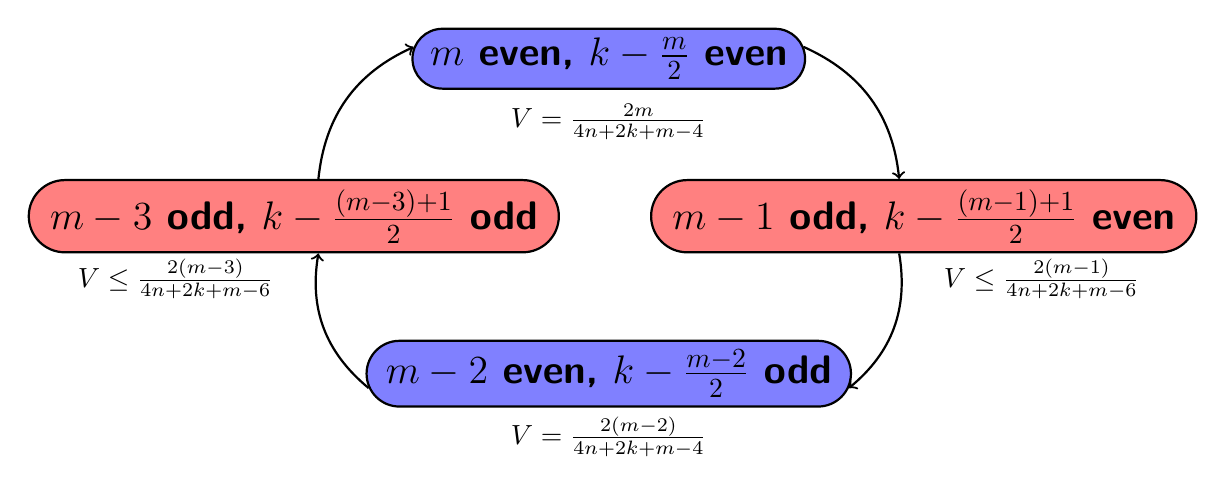
\begin{tikzpicture}[-,auto,node distance=1.5cm,
                    thick,main node/.style={rounded rectangle,fill=white,draw,font=\sffamily\Large\bfseries}]
                 
 \node[main node,fill=blue!50] (1) at (0,0) {$m$ even, $k-\frac{m}{2}$ even};
 
 \node (value1) at (0,-0.8) {$V = \frac{2m}{4n+2k+m-4}$}; 
 
 \node[main node,fill=red!50] (2) at (4,-2) {$m-1$ odd, $k-\frac{(m-1)+1}{2}$ even};
 
 \node (value2) at (5.5,-2.8) {$V \leq \frac{2(m-1)}{4n+2k+m-6}$};
 
 \node[main node,fill=blue!50] (3) at (0,-4) {$m-2$ even, $k-\frac{m-2}{2}$ odd};
 
 \node (value2) at (0,-4.8) {$V = \frac{2(m-2)}{4n+2k+m-4}$}; 
 
 \node[main node,fill=red!50] (4) at (-4,-2) {$m-3$ odd, $k-\frac{(m-3)+1}{2}$ odd};
 
 \node (value2) at (-5.5,-2.8) {$V \leq \frac{2(m-3)}{4n+2k+m-6}$}; 
 
 
 
  \path[->,bend left,every node/.style={font=\sffamily}]
    (1) edge (2)
    (2) edge (3)
    (3) edge (4)
    (4) edge (1);
                    
\end{tikzpicture}                    
\end{center}
\caption{Cycle of $m$ decreasing}
\end{myfigure}


\subsection{Extending even solution}
The question is now is it possible to extend the even solution as described above when $m \leq 2(n-1)$ is odd. We note that in the cycle we can see the just look at making $1$ less attacks to give an attackers bound. Let $m=m'-1$ then we assume we can just simply take one attack away from node $1$ attacks and we are away.

We can notice that the combinatorial improvement does much worse due to the $\floor{\frac{m}{2}}$ part, we may decide a different improvement, following similiar principles is needed.

\subsection{Combinatorial loop improvement}
We alter the idea of using end-ensuring cycles on the set of $S$ (please note we will deal with only the case of $R \neq \emptyset$ (as that is what we need this for odd m). We will now improve the $n-1$ nodes by using a cycle of length $m+1$ (note we will be covering the case where $m$ is odd), then when played this cycle has a probability of catching the attacker of $\frac{m}{m+1} \equiv \frac{m}{m'}$.

Now just like before we will need to play a collection of all combinations of such cycles, each cycle has a choice of $\frac{m'}{2}$ end points to visit. So we have a total of $\left( \begin{array}{c}
n-1 \\
\frac{m'}{2} \\
\end{array} \right)
$
and  $\left( \begin{array}{c}
n-2 \\
\frac{m'}{2}-1 \\
\end{array} \right)
$
contain any given end point. Hence we have $\frac{\left( \begin{array}{c}
n-1 \\
\frac{m'}{2} \\
\end{array} \right)}{\left( \begin{array}{c}
n-2 \\
\frac{m'}{2}-1 \\
\end{array} \right)}=
\frac{m'}{2(n-1)}
$
Hence when we play this strategy with probability $q$, we improve each end with a probability of $q \times \frac{m'}{2(n-1)}$.

We will give the details and the bounds in the appendix \ref{appendix: Combinatorial loop improvement analysis}

But here we note that getting such a bound analgous to before is possible.

\subsection{Odd solution}
By using the combinatorial loop improvement when $m$ is odd, then we can get a bound of $V \geq \frac{m}{2(n+k)+m+2(n-1)}$. We claim we can also get $V \leq \frac{2m}{2(n+k)+m+2(n-1)}$, now we know the solution for $m'=m+1$ which is $V \leq \frac{2m'}{2(n+k)+m'+2(n-1)}=\frac{2m+2}{2(n+k)+m+1+2(n-1)}$ , we now want to suggest moving $1$ attack from the system

Let us say that $m=5$ in $S_{7}^{9}$ then we have by placing attacks that $V \leq \frac{2m}{2(n+k)+m+2(n-1)-1}$ (if $k-\frac{m+1}{2}$ is odd) or $V \leq \frac{2m}{2(n+k)+m+2(n-1)-3}$ (if $k-\frac{m+1}{2}$ is even) 

i.e as $9-3=6$ even we get $V \leq \frac{10}{32+5+10-3}=\frac{10}{48}=\frac{5}{24}$ , now the combinatorial improvement gives me $V \geq \frac{10}{32+5+10}=\frac{5}{24.5}$. So from our $m=6$ solution which would have even $k-\frac{6}{2}$, in which we got $V=\frac{6}{16+3+6}=\frac{6}{25}$, so from here it should be a case of removing an attack


A solution to get the combinatorial loop bound can be made by making a particular type of attack. Looking at a particular example on $S_{7}^{5}$.


\begin{myfigure}
\begin{center}
\resizebox{1\linewidth}{!}{
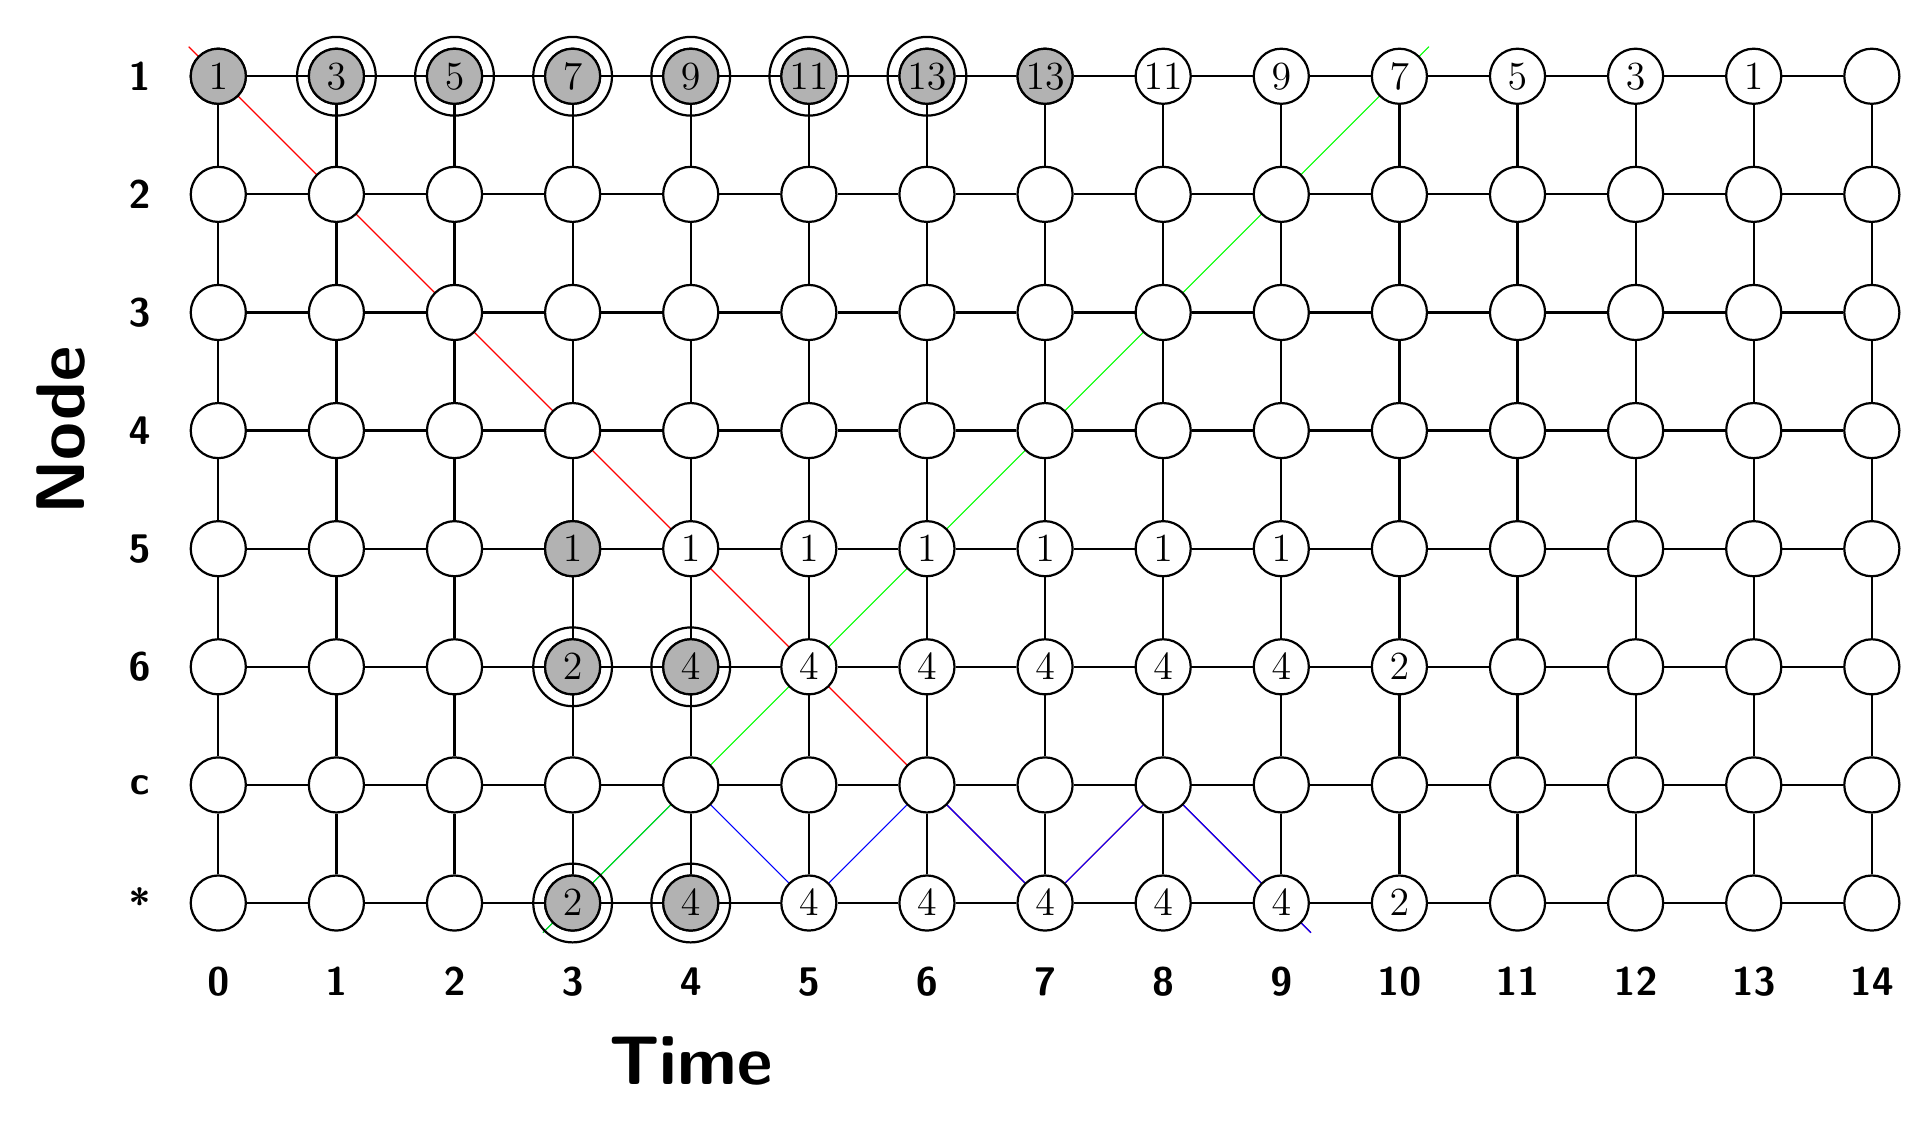
\begin{tikzpicture}[-,auto,node distance=1cm,
                    thick,main node/.style={circle,fill=white,draw,font=\sffamily\Large\bfseries,minimum size=0.7cm}]
 \foreach \x in {0,...,14}
    \foreach \y in {0,...,7} 
       {\pgfmathtruncatemacro{\label}{\x - 5 *  \y +21}
       \node [main node]  (\x\y) at (1.5*\x,1.5*\y) {};} 

  \foreach \x in {0,...,13}
   \foreach \y in {0,...,6}
    \pgfmathtruncatemacro{\za}{\y+1}
    \pgfmathtruncatemacro{\zb}{\x+1}
      \draw (\x\y)--(\x\za) (\x\y)--(\zb\y) ;
      
   \foreach \x in {0,...,13}
    \pgfmathtruncatemacro{\zb}{\x+1}
      \draw (\x7) -- (\zb7);
      
   \foreach \y in {0,...,6}
     \pgfmathtruncatemacro{\za}{\y+1} 
        \draw (14\y) -- (14\za);
        
        
%Labeling to the sides
  \foreach \y in {2,...,7}
   \pgfmathtruncatemacro{\label}{8-\y}
   \node[font=\sffamily\Large\bfseries] (Label\y) [shift={(-1,0)}] at (0\y) {\label};       
   
   \node[font=\sffamily\Large\bfseries] (Label) [shift={(-1,0)}] at (01) {c};
   \node[font=\sffamily\Large\bfseries] (Label) [shift={(-1,0)}] at (00) {*};
   
   \node[font=\sffamily\Huge\bfseries] (Axis) [shift={(-2,0)},rotate=90] at (04) {Node};

   \foreach \x in {0,...,14}
    \node[font=\sffamily\Large\bfseries] (Timelabel\x) [shift={(0,-1)}] at (\x0) {\x};
    
   \node[font=\sffamily\Huge\bfseries] (Axis) [shift={(0,-2)}] at (40) {Time};
    
    
%Adding in top attacks        
   \node[main node,fill=gray!60] (07) at (07) {};    
   
   \foreach \x in {1,...,6}
   \node[main node,fill=gray!60] (\x7) at (\x7) {};
   
   \foreach \x in {1,...,6}    
   \node[circle,draw,minimum size=1cm] (Attack\x) at (\x7) {};
   
   \node[main node,fill=gray!60] (77) at (77) {};    
   

   
   %Attack numbers
    \node[font=\sffamily\Large\bfseries] (AttackNumber1)  at (07) {$1$};
    \node[font=\sffamily\Large\bfseries] (AttackNumber1)  at (17) {$3$}; 
    \node[font=\sffamily\Large\bfseries] (AttackNumber1)  at (27) {$5$}; 
    \node[font=\sffamily\Large\bfseries] (AttackNumber1)  at (37) {$7$}; 
    \node[font=\sffamily\Large\bfseries] (AttackNumber1)  at (47) {$9$}; 
    \node[font=\sffamily\Large\bfseries] (AttackNumber1)  at (57) {$11$}; 
    \node[font=\sffamily\Large\bfseries] (AttackNumber1)  at (67) {$13$}; 
    \node[font=\sffamily\Large\bfseries] (AttackNumber1)  at (77) {$13$}; 
    \node[font=\sffamily\Large\bfseries] (AttackNumber1)  at (87) {$11$}; 
    \node[font=\sffamily\Large\bfseries] (AttackNumber1)  at (97) {$9$};
    \node[font=\sffamily\Large\bfseries] (AttackNumber1)  at (107) {$7$}; 
    \node[font=\sffamily\Large\bfseries] (AttackNumber1)  at (117) {$5$};
    \node[font=\sffamily\Large\bfseries] (AttackNumber1)  at (127) {$3$};    
    \node[font=\sffamily\Large\bfseries] (AttackNumber1)  at (137) {$1$};          
   
%Adding in middle attacks
  \node[main node,fill=gray!60] (33) at (33) {};
  
  \node[main node,fill=gray!60] (32) at (32) {};
  \node[circle,draw,minimum size=1cm] (Attack0) at (32) {};
  
  \node[main node,fill=gray!60] (42) at (42) {};
  \node[circle,draw,minimum size=1cm] (Attack0) at (42) {};
     
    %Attack numbers
    \node[font=\sffamily\Large\bfseries] (AttackNumber1)  at (33) {$1$};
    \node[font=\sffamily\Large\bfseries] (AttackNumber1)  at (43) {$1$}; 
    \node[font=\sffamily\Large\bfseries] (AttackNumber1)  at (53) {$1$}; 
    \node[font=\sffamily\Large\bfseries] (AttackNumber1)  at (63) {$1$}; 
    \node[font=\sffamily\Large\bfseries] (AttackNumber1)  at (73) {$1$}; 
    \node[font=\sffamily\Large\bfseries] (AttackNumber1)  at (83) {$1$};
    \node[font=\sffamily\Large\bfseries] (AttackNumber1)  at (93) {$1$};
     
    \node[font=\sffamily\Large\bfseries] (AttackNumber1)  at (32) {$2$}; 
    \node[font=\sffamily\Large\bfseries] (AttackNumber1)  at (42) {$4$}; 
    \node[font=\sffamily\Large\bfseries] (AttackNumber1)  at (52) {$4$}; 
    \node[font=\sffamily\Large\bfseries] (AttackNumber1)  at (62) {$4$}; 
    \node[font=\sffamily\Large\bfseries] (AttackNumber1)  at (72) {$4$}; 
    \node[font=\sffamily\Large\bfseries] (AttackNumber1)  at (82) {$4$}; 
    \node[font=\sffamily\Large\bfseries] (AttackNumber1)  at (92) {$4$}; 
    \node[font=\sffamily\Large\bfseries] (AttackNumber1)  at (102) {$2$};
    
%Adding bottom attacks

  \node[main node,fill=gray!60] (30) at (30) {};
  \node[circle,draw,minimum size=1cm] (Attack0) at (30) {};
  
  \node[main node,fill=gray!60] (40) at (40) {};
  \node[circle,draw,minimum size=1cm] (Attack0) at (40) {};
 
    %Attack numbers
    \node[font=\sffamily\Large\bfseries] (AttackNumber1)  at (30) {$2$}; 
    \node[font=\sffamily\Large\bfseries] (AttackNumber1)  at (40) {$4$}; 
    \node[font=\sffamily\Large\bfseries] (AttackNumber1)  at (50) {$4$}; 
    \node[font=\sffamily\Large\bfseries] (AttackNumber1)  at (60) {$4$}; 
    \node[font=\sffamily\Large\bfseries] (AttackNumber1)  at (70) {$4$}; 
    \node[font=\sffamily\Large\bfseries] (AttackNumber1)  at (80) {$4$}; 
    \node[font=\sffamily\Large\bfseries] (AttackNumber1)  at (90) {$4$}; 
    \node[font=\sffamily\Large\bfseries] (AttackNumber1)  at (100) {$2$};       
        
                 
%Some example lines drawn
\begin{scope}[on background layer]
\node (a)[shift={(-0.5,0.5)}] at (07) {};
\node (b)[shift={(0.5,-0.5)}] at (90) {};
\draw[color=red] (a) -- (70) (70)--(81) (81)--(b);

\node (c)[shift={(-0.5,-0.5)}] at (30) {};
\node (d)[shift={(0.5,0.5)}] at (94) {};
\draw[color=blue] (c) -- (41) (41)--(50) (50)--(61) (61)--(70) (70)--(81) (81)--(b);

\node (d) [shift={(0.5,0.5)}] at (107) {};
\draw[color=green] (c) -- (d);

\end{scope}

                   
\end{tikzpicture}
}
\end{center}
\caption{Grid solution of $m=7$ on $S_{7}^{5}$ with two example paths}
\end{myfigure}

\begin{note}
In the picture we are using a double type attack as we need whole number to get our bound of $V \leq \frac{14}{43}$
\end{note}

\textbf{Solution just after $m$ even $k-\frac{m}{2}$ odd}
In this $m$ is odd and $k-\frac{m+1}{2}$ is still odd
In general this type of attack will make $2m$ attacks at node $1$ and $4(n-1)$ (in total) attacks at the $*$ nodes, it will also make $4*\ceil{\frac{k+1-\frac{m+1}{2}-1}{2}}+1=4*\ceil{\frac{k-\frac{m+1}{2}}{2}}+1=4*(\frac{k-\frac{m+1}{2}+1}{2})+1=2k-m-1+2+1=2k-m+2$ attacks in the middle. So in total $2m+4(n-1)+2k-m+2=2(n+k)+m+2(n-1)$. Hence the bound of $V \leq \frac{2m}{2(n+k)+m+2(n-1)}$ is achieved and this part of the cycle is solved

\begin{myfigure}
\begin{center}
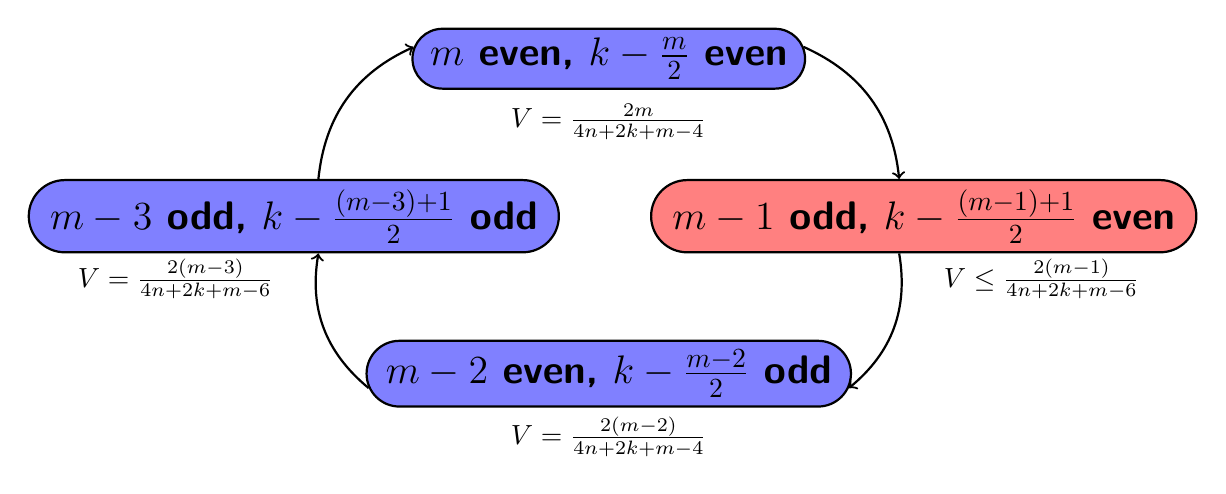
\begin{tikzpicture}[-,auto,node distance=1.5cm,
                    thick,main node/.style={rounded rectangle,fill=white,draw,font=\sffamily\Large\bfseries}]
                 
 \node[main node,fill=blue!50] (1) at (0,0) {$m$ even, $k-\frac{m}{2}$ even};
 
 \node (value1) at (0,-0.8) {$V = \frac{2m}{4n+2k+m-4}$}; 
 
 \node[main node,fill=red!50] (2) at (4,-2) {$m-1$ odd, $k-\frac{(m-1)+1}{2}$ even};
 
 \node (value2) at (5.5,-2.8) {$V \leq \frac{2(m-1)}{4n+2k+m-6}$};
 
 \node[main node,fill=blue!50] (3) at (0,-4) {$m-2$ even, $k-\frac{m-2}{2}$ odd};
 
 \node (value2) at (0,-4.8) {$V = \frac{2(m-2)}{4n+2k+m-4}$}; 
 
 \node[main node,fill=blue!50] (4) at (-4,-2) {$m-3$ odd, $k-\frac{(m-3)+1}{2}$ odd};
 
 \node (value2) at (-5.5,-2.8) {$V = \frac{2(m-3)}{4n+2k+m-6}$}; 
 
 
 
  \path[->,bend left,every node/.style={font=\sffamily}]
    (1) edge (2)
    (2) edge (3)
    (3) edge (4)
    (4) edge (1);
                    
\end{tikzpicture}                    
\end{center}
\caption{Cycle of $m$ decreasing}
\end{myfigure}

\textbf{Solution just after $m$ even $k-\frac{m}{2}$ even}
So here $m$ is odd and $k-\frac{m+1}{2}$ is even. We again need to look at augementing the strategy 

Again we present a strategy on $S_{7}^{5}$ as an insight

\begin{myfigure}
\begin{center}
\resizebox{1\linewidth}{!}{
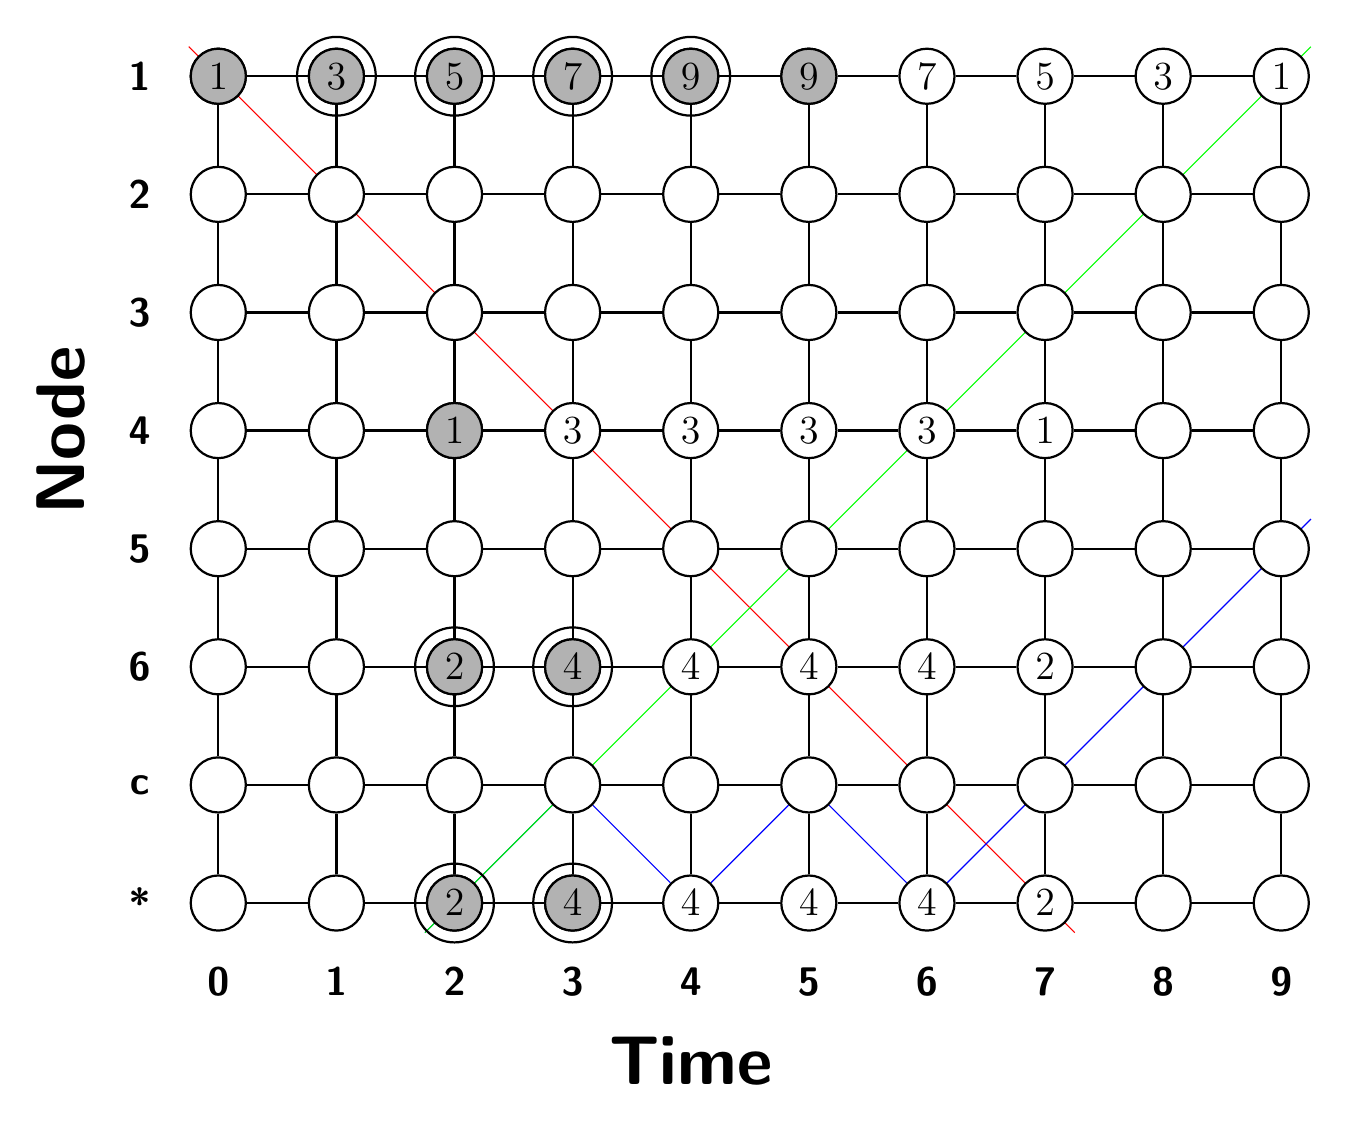
\begin{tikzpicture}[-,auto,node distance=1cm,
                    thick,main node/.style={circle,fill=white,draw,font=\sffamily\Large\bfseries,minimum size=0.7cm}]
 \foreach \x in {0,...,9}
    \foreach \y in {0,...,7} 
       {\pgfmathtruncatemacro{\label}{\x - 5 *  \y +21}
       \node [main node]  (\x\y) at (1.5*\x,1.5*\y) {};} 

  \foreach \x in {0,...,8}
   \foreach \y in {0,...,6}
    \pgfmathtruncatemacro{\za}{\y+1}
    \pgfmathtruncatemacro{\zb}{\x+1}
      \draw (\x\y)--(\x\za) (\x\y)--(\zb\y) ;
      
   \foreach \x in {0,...,8}
    \pgfmathtruncatemacro{\zb}{\x+1}
      \draw (\x7) -- (\zb7);
      
   \foreach \y in {0,...,6}
     \pgfmathtruncatemacro{\za}{\y+1} 
        \draw (9\y) -- (9\za);
        
        
%Labeling to the sides
  \foreach \y in {2,...,7}
   \pgfmathtruncatemacro{\label}{8-\y}
   \node[font=\sffamily\Large\bfseries] (Label\y) [shift={(-1,0)}] at (0\y) {\label};       
   
   \node[font=\sffamily\Large\bfseries] (Label) [shift={(-1,0)}] at (01) {c};
   \node[font=\sffamily\Large\bfseries] (Label) [shift={(-1,0)}] at (00) {*};
   
   \node[font=\sffamily\Huge\bfseries] (Axis) [shift={(-2,0)},rotate=90] at (04) {Node};

   \foreach \x in {0,...,9}
    \node[font=\sffamily\Large\bfseries] (Timelabel\x) [shift={(0,-1)}] at (\x0) {\x};
    
   \node[font=\sffamily\Huge\bfseries] (Axis) [shift={(0,-2)}] at (40) {Time};
    
    
%Adding in top attacks        
   \node[main node,fill=gray!60] (07) at (07) {};    
   
   \foreach \x in {1,...,4}
   \node[main node,fill=gray!60] (\x7) at (\x7) {};
   
   \foreach \x in {1,...,4}    
   \node[circle,draw,minimum size=1cm] (Attack\x) at (\x7) {};
   
   \node[main node,fill=gray!60] (57) at (57) {};    
   

   
   %Attack numbers
    \node[font=\sffamily\Large\bfseries] (AttackNumber1)  at (07) {$1$};
    \node[font=\sffamily\Large\bfseries] (AttackNumber1)  at (17) {$3$}; 
    \node[font=\sffamily\Large\bfseries] (AttackNumber1)  at (27) {$5$}; 
    \node[font=\sffamily\Large\bfseries] (AttackNumber1)  at (37) {$7$}; 
    \node[font=\sffamily\Large\bfseries] (AttackNumber1)  at (47) {$9$}; 
    \node[font=\sffamily\Large\bfseries] (AttackNumber1)  at (57) {$9$}; 
    \node[font=\sffamily\Large\bfseries] (AttackNumber1)  at (67) {$7$}; 
    \node[font=\sffamily\Large\bfseries] (AttackNumber1)  at (77) {$5$}; 
    \node[font=\sffamily\Large\bfseries] (AttackNumber1)  at (87) {$3$};
    \node[font=\sffamily\Large\bfseries] (AttackNumber1)  at (97) {$1$};  
         
   
%Adding in middle attacks
  \node[main node,fill=gray!60] (24) at (24) {};
  
  \node[main node,fill=gray!60] (22) at (22) {};
  \node[circle,draw,minimum size=1cm] (Attack0) at (22) {};
  
  \node[main node,fill=gray!60] (32) at (32) {};
  \node[circle,draw,minimum size=1cm] (Attack0) at (32) {};
     
    %Attack numbers
    \node[font=\sffamily\Large\bfseries] (AttackNumber1)  at (24) {$1$};
    \node[font=\sffamily\Large\bfseries] (AttackNumber1)  at (34) {$3$}; 
    \node[font=\sffamily\Large\bfseries] (AttackNumber1)  at (44) {$3$}; 
    \node[font=\sffamily\Large\bfseries] (AttackNumber1)  at (54) {$3$}; 
    \node[font=\sffamily\Large\bfseries] (AttackNumber1)  at (64) {$3$}; 
    \node[font=\sffamily\Large\bfseries] (AttackNumber1)  at (74) {$1$};
     
    \node[font=\sffamily\Large\bfseries] (AttackNumber1)  at (22) {$2$}; 
    \node[font=\sffamily\Large\bfseries] (AttackNumber1)  at (32) {$4$}; 
    \node[font=\sffamily\Large\bfseries] (AttackNumber1)  at (42) {$4$}; 
    \node[font=\sffamily\Large\bfseries] (AttackNumber1)  at (52) {$4$}; 
    \node[font=\sffamily\Large\bfseries] (AttackNumber1)  at (62) {$4$}; 
    \node[font=\sffamily\Large\bfseries] (AttackNumber1)  at (72) {$2$}; 

    
%Adding bottom attacks

  \node[main node,fill=gray!60] (20) at (20) {};
  \node[circle,draw,minimum size=1cm] (Attack0) at (20) {};
  
  \node[main node,fill=gray!60] (30) at (30) {};
  \node[circle,draw,minimum size=1cm] (Attack0) at (30) {};
 
    %Attack numbers
    \node[font=\sffamily\Large\bfseries] (AttackNumber1)  at (20) {$2$}; 
    \node[font=\sffamily\Large\bfseries] (AttackNumber1)  at (30) {$4$}; 
    \node[font=\sffamily\Large\bfseries] (AttackNumber1)  at (40) {$4$}; 
    \node[font=\sffamily\Large\bfseries] (AttackNumber1)  at (50) {$4$}; 
    \node[font=\sffamily\Large\bfseries] (AttackNumber1)  at (60) {$4$}; 
    \node[font=\sffamily\Large\bfseries] (AttackNumber1)  at (70) {$2$}; 
     
        
                 
%Some example lines drawn
\begin{scope}[on background layer]
\node (a)[shift={(-0.5,0.5)}] at (07) {};
\node (b)[shift={(0.5,-0.5)}] at (70) {};
\draw[color=red] (a) -- (b);

\node (c)[shift={(-0.5,-0.5)}] at (20) {};
\node (d)[shift={(0.5,0.5)}] at (93) {};
\draw[color=blue] (c) -- (31) (31)--(40) (40)--(51) (51)--(60) (60)--(d);

\node (e) [shift={(0.5,0.5)}] at (97) {};
\draw[color=green] (c) -- (e);

\end{scope}

                   
\end{tikzpicture}
}
\end{center}
\caption{Grid solution of $m=5$ on $S_{7}^{5}$ with two example paths}
\end{myfigure}

Again we now reason that we make $2m$ attacks at node $1$ and $4(n-1)$ (in total) attacks at $*$ nodes and in the middle we have $4*\ceil{\frac{k+1-\frac{m+1}{2}-2}{2}}+3=4*\ceil{\frac{k-\frac{m+1}{2}-1}{2}}+3=4*(\frac{k-\frac{m+1}{2}-1+1}{2})+3=2k-m-1+3=2k-m+2$ , for a total of $2m+4(n-1)+2k-m+2=2(n+k)+m+2(n-1)$ attacks.
Giving again the bound of $V \leq \frac{2m}{2(n+k)+m+2(n-1)}$ matching with the combinatorial loop bound.

\subsection{Solution for $m \leq 2(n-1)$}
Know we align ourselves with the solution for $m=2k-1$ and $m=2k-2$ by using these type ideas. However $m=2k+1$ and $m=2k$ need to still be kept separate. But below this and before $m=2$ or $m=1$ we now know the answer, that it follows the combinatorial improvment (for $V=\frac{2m}{2(n+k)+m+2(n-1)}$

\begin{myfigure}
% Created by tikzDevice version 0.10.1 on 2017-12-05 18:40:51
% !TEX encoding = UTF-8 Unicode
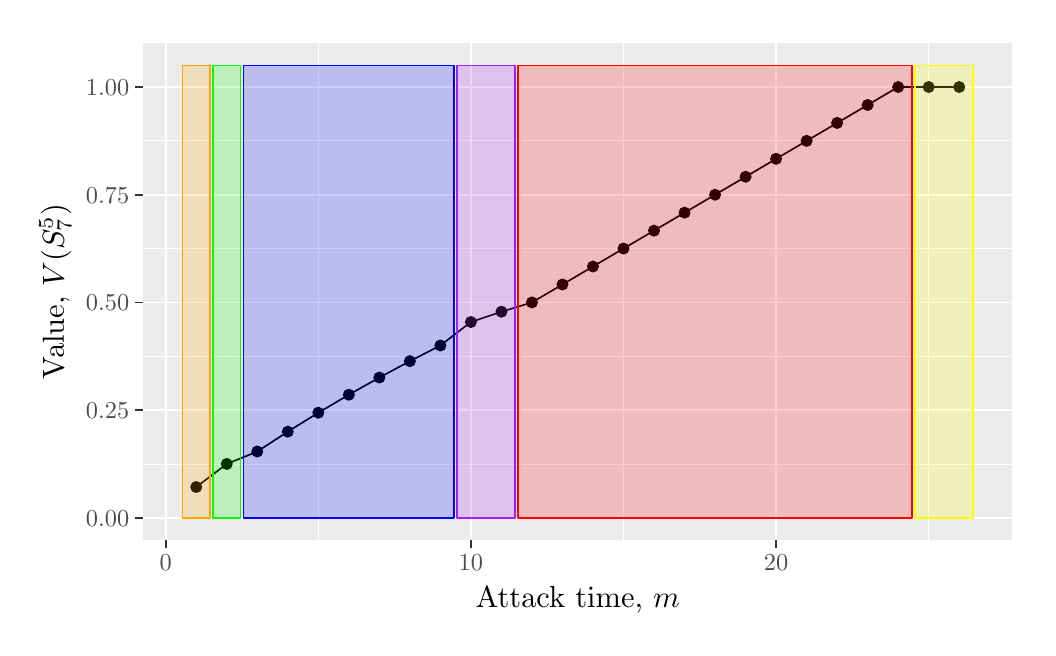
\begin{tikzpicture}[x=1pt,y=1pt]
\definecolor{fillColor}{RGB}{255,255,255}
\path[use as bounding box,fill=fillColor,fill opacity=0.00] (0,0) rectangle (361.35,216.81);
\begin{scope}
\path[clip] (  0.00,  0.00) rectangle (361.35,216.81);
\definecolor{drawColor}{RGB}{255,255,255}
\definecolor{fillColor}{RGB}{255,255,255}

\path[draw=drawColor,line width= 0.6pt,line join=round,line cap=round,fill=fillColor] (  0.00,  0.00) rectangle (361.35,216.81);
\end{scope}
\begin{scope}
\path[clip] ( 41.67, 31.53) rectangle (355.85,211.31);
\definecolor{fillColor}{gray}{0.92}

\path[fill=fillColor] ( 41.67, 31.53) rectangle (355.85,211.31);
\definecolor{drawColor}{RGB}{255,255,255}

\path[draw=drawColor,line width= 0.3pt,line join=round] ( 41.67, 59.16) --
	(355.85, 59.16);

\path[draw=drawColor,line width= 0.3pt,line join=round] ( 41.67, 98.07) --
	(355.85, 98.07);

\path[draw=drawColor,line width= 0.3pt,line join=round] ( 41.67,136.99) --
	(355.85,136.99);

\path[draw=drawColor,line width= 0.3pt,line join=round] ( 41.67,175.90) --
	(355.85,175.90);

\path[draw=drawColor,line width= 0.3pt,line join=round] (105.02, 31.53) --
	(105.02,211.31);

\path[draw=drawColor,line width= 0.3pt,line join=round] (215.30, 31.53) --
	(215.30,211.31);

\path[draw=drawColor,line width= 0.3pt,line join=round] (325.58, 31.53) --
	(325.58,211.31);

\path[draw=drawColor,line width= 0.6pt,line join=round] ( 41.67, 39.70) --
	(355.85, 39.70);

\path[draw=drawColor,line width= 0.6pt,line join=round] ( 41.67, 78.62) --
	(355.85, 78.62);

\path[draw=drawColor,line width= 0.6pt,line join=round] ( 41.67,117.53) --
	(355.85,117.53);

\path[draw=drawColor,line width= 0.6pt,line join=round] ( 41.67,156.44) --
	(355.85,156.44);

\path[draw=drawColor,line width= 0.6pt,line join=round] ( 41.67,195.36) --
	(355.85,195.36);

\path[draw=drawColor,line width= 0.6pt,line join=round] ( 49.88, 31.53) --
	( 49.88,211.31);

\path[draw=drawColor,line width= 0.6pt,line join=round] (160.16, 31.53) --
	(160.16,211.31);

\path[draw=drawColor,line width= 0.6pt,line join=round] (270.44, 31.53) --
	(270.44,211.31);
\definecolor{drawColor}{RGB}{0,0,0}
\definecolor{fillColor}{RGB}{0,0,0}

\path[draw=drawColor,line width= 0.4pt,line join=round,line cap=round,fill=fillColor] (325.58,195.36) circle (  1.96);

\path[draw=drawColor,line width= 0.4pt,line join=round,line cap=round,fill=fillColor] (336.61,195.36) circle (  1.96);

\path[draw=drawColor,line width= 0.4pt,line join=round,line cap=round,fill=fillColor] (182.22,117.53) circle (  1.96);

\path[draw=drawColor,line width= 0.4pt,line join=round,line cap=round,fill=fillColor] (193.24,124.01) circle (  1.96);

\path[draw=drawColor,line width= 0.4pt,line join=round,line cap=round,fill=fillColor] (204.27,130.50) circle (  1.96);

\path[draw=drawColor,line width= 0.4pt,line join=round,line cap=round,fill=fillColor] (215.30,136.99) circle (  1.96);

\path[draw=drawColor,line width= 0.4pt,line join=round,line cap=round,fill=fillColor] (226.33,143.47) circle (  1.96);

\path[draw=drawColor,line width= 0.4pt,line join=round,line cap=round,fill=fillColor] (237.36,149.96) circle (  1.96);

\path[draw=drawColor,line width= 0.4pt,line join=round,line cap=round,fill=fillColor] (248.38,156.44) circle (  1.96);

\path[draw=drawColor,line width= 0.4pt,line join=round,line cap=round,fill=fillColor] (259.41,162.93) circle (  1.96);

\path[draw=drawColor,line width= 0.4pt,line join=round,line cap=round,fill=fillColor] (270.44,169.41) circle (  1.96);

\path[draw=drawColor,line width= 0.4pt,line join=round,line cap=round,fill=fillColor] (281.47,175.90) circle (  1.96);

\path[draw=drawColor,line width= 0.4pt,line join=round,line cap=round,fill=fillColor] (292.49,182.38) circle (  1.96);

\path[draw=drawColor,line width= 0.4pt,line join=round,line cap=round,fill=fillColor] (303.52,188.87) circle (  1.96);

\path[draw=drawColor,line width= 0.4pt,line join=round,line cap=round,fill=fillColor] (314.55,195.36) circle (  1.96);

\path[draw=drawColor,line width= 0.4pt,line join=round,line cap=round,fill=fillColor] (160.16,110.45) circle (  1.96);

\path[draw=drawColor,line width= 0.4pt,line join=round,line cap=round,fill=fillColor] (171.19,114.15) circle (  1.96);

\path[draw=drawColor,line width= 0.4pt,line join=round,line cap=round,fill=fillColor] ( 82.97, 63.65) circle (  1.96);

\path[draw=drawColor,line width= 0.4pt,line join=round,line cap=round,fill=fillColor] ( 93.99, 70.83) circle (  1.96);

\path[draw=drawColor,line width= 0.4pt,line join=round,line cap=round,fill=fillColor] (105.02, 77.67) circle (  1.96);

\path[draw=drawColor,line width= 0.4pt,line join=round,line cap=round,fill=fillColor] (116.05, 84.17) circle (  1.96);

\path[draw=drawColor,line width= 0.4pt,line join=round,line cap=round,fill=fillColor] (127.08, 90.38) circle (  1.96);

\path[draw=drawColor,line width= 0.4pt,line join=round,line cap=round,fill=fillColor] (138.10, 96.30) circle (  1.96);

\path[draw=drawColor,line width= 0.4pt,line join=round,line cap=round,fill=fillColor] (149.13,101.96) circle (  1.96);

\path[draw=drawColor,line width= 0.4pt,line join=round,line cap=round,fill=fillColor] ( 60.91, 50.82) circle (  1.96);

\path[draw=drawColor,line width= 0.4pt,line join=round,line cap=round,fill=fillColor] ( 71.94, 59.16) circle (  1.96);

\path[draw=drawColor,line width= 0.6pt,line join=round] ( 60.91, 50.82) --
	( 71.94, 59.16) --
	( 82.97, 63.65) --
	( 93.99, 70.83) --
	(105.02, 77.67) --
	(116.05, 84.17) --
	(127.08, 90.38) --
	(138.10, 96.30) --
	(149.13,101.96) --
	(160.16,110.45) --
	(171.19,114.15) --
	(182.22,117.53) --
	(193.24,124.01) --
	(204.27,130.50) --
	(215.30,136.99) --
	(226.33,143.47) --
	(237.36,149.96) --
	(248.38,156.44) --
	(259.41,162.93) --
	(270.44,169.41) --
	(281.47,175.90) --
	(292.49,182.38) --
	(303.52,188.87) --
	(314.55,195.36) --
	(325.58,195.36) --
	(336.61,195.36);
\definecolor{drawColor}{RGB}{255,255,0}
\definecolor{fillColor}{RGB}{255,255,0}

\path[draw=drawColor,line width= 0.6pt,line join=round,fill=fillColor,fill opacity=0.20] (320.62, 39.70) rectangle (341.57,203.14);
\definecolor{drawColor}{RGB}{255,0,0}
\definecolor{fillColor}{RGB}{255,0,0}

\path[draw=drawColor,line width= 0.6pt,line join=round,fill=fillColor,fill opacity=0.20] (177.25, 39.70) rectangle (319.51,203.14);
\definecolor{drawColor}{RGB}{160,32,240}
\definecolor{fillColor}{RGB}{160,32,240}

\path[draw=drawColor,line width= 0.6pt,line join=round,fill=fillColor,fill opacity=0.20] (155.20, 39.70) rectangle (176.15,203.14);
\definecolor{drawColor}{RGB}{0,0,255}
\definecolor{fillColor}{RGB}{0,0,255}

\path[draw=drawColor,line width= 0.6pt,line join=round,fill=fillColor,fill opacity=0.20] ( 78.00, 39.70) rectangle (154.10,203.14);
\definecolor{drawColor}{RGB}{0,255,0}
\definecolor{fillColor}{RGB}{0,255,0}

\path[draw=drawColor,line width= 0.6pt,line join=round,fill=fillColor,fill opacity=0.20] ( 66.98, 39.70) rectangle ( 76.90,203.14);
\definecolor{drawColor}{RGB}{255,165,0}
\definecolor{fillColor}{RGB}{255,165,0}

\path[draw=drawColor,line width= 0.6pt,line join=round,fill=fillColor,fill opacity=0.20] ( 55.95, 39.70) rectangle ( 65.87,203.14);
\end{scope}
\begin{scope}
\path[clip] (  0.00,  0.00) rectangle (361.35,216.81);
\definecolor{drawColor}{gray}{0.30}

\node[text=drawColor,anchor=base east,inner sep=0pt, outer sep=0pt, scale=  0.88] at ( 36.72, 36.67) {0.00};

\node[text=drawColor,anchor=base east,inner sep=0pt, outer sep=0pt, scale=  0.88] at ( 36.72, 75.59) {0.25};

\node[text=drawColor,anchor=base east,inner sep=0pt, outer sep=0pt, scale=  0.88] at ( 36.72,114.50) {0.50};

\node[text=drawColor,anchor=base east,inner sep=0pt, outer sep=0pt, scale=  0.88] at ( 36.72,153.41) {0.75};

\node[text=drawColor,anchor=base east,inner sep=0pt, outer sep=0pt, scale=  0.88] at ( 36.72,192.33) {1.00};
\end{scope}
\begin{scope}
\path[clip] (  0.00,  0.00) rectangle (361.35,216.81);
\definecolor{drawColor}{gray}{0.20}

\path[draw=drawColor,line width= 0.6pt,line join=round] ( 38.92, 39.70) --
	( 41.67, 39.70);

\path[draw=drawColor,line width= 0.6pt,line join=round] ( 38.92, 78.62) --
	( 41.67, 78.62);

\path[draw=drawColor,line width= 0.6pt,line join=round] ( 38.92,117.53) --
	( 41.67,117.53);

\path[draw=drawColor,line width= 0.6pt,line join=round] ( 38.92,156.44) --
	( 41.67,156.44);

\path[draw=drawColor,line width= 0.6pt,line join=round] ( 38.92,195.36) --
	( 41.67,195.36);
\end{scope}
\begin{scope}
\path[clip] (  0.00,  0.00) rectangle (361.35,216.81);
\definecolor{drawColor}{gray}{0.20}

\path[draw=drawColor,line width= 0.6pt,line join=round] ( 49.88, 28.78) --
	( 49.88, 31.53);

\path[draw=drawColor,line width= 0.6pt,line join=round] (160.16, 28.78) --
	(160.16, 31.53);

\path[draw=drawColor,line width= 0.6pt,line join=round] (270.44, 28.78) --
	(270.44, 31.53);
\end{scope}
\begin{scope}
\path[clip] (  0.00,  0.00) rectangle (361.35,216.81);
\definecolor{drawColor}{gray}{0.30}

\node[text=drawColor,anchor=base,inner sep=0pt, outer sep=0pt, scale=  0.88] at ( 49.88, 20.52) {0};

\node[text=drawColor,anchor=base,inner sep=0pt, outer sep=0pt, scale=  0.88] at (160.16, 20.52) {10};

\node[text=drawColor,anchor=base,inner sep=0pt, outer sep=0pt, scale=  0.88] at (270.44, 20.52) {20};
\end{scope}
\begin{scope}
\path[clip] (  0.00,  0.00) rectangle (361.35,216.81);
\definecolor{drawColor}{RGB}{0,0,0}

\node[text=drawColor,anchor=base,inner sep=0pt, outer sep=0pt, scale=  1.10] at (198.76,  7.44) {Attack time, $m$};
\end{scope}
\begin{scope}
\path[clip] (  0.00,  0.00) rectangle (361.35,216.81);
\definecolor{drawColor}{RGB}{0,0,0}

\node[text=drawColor,rotate= 90.00,anchor=base,inner sep=0pt, outer sep=0pt, scale=  1.10] at ( 13.08,121.42) {Value, $V(S_{ 7 }^{ 5 })$};
\end{scope}
\end{tikzpicture}

\caption{A graph of Values of $S_{7}^{5}$ for various m}
\end{myfigure}

Hence we have a complete solution if $2k \leq 2(n-1) \iff k \leq n-1$. Otherwise we will have a gap in our current solution till it $m \leq 2(n-1)$. 


\subsection{Solution when $m > 2(n-1)$}
We suggest that we may seek answers along the line of the combinatorial improvement $V \geq \frac{2m}{2n+2k+2m}$ . We will first note that $2n+2k+2m > 2n+m+2(n-1)+2k=2(n+k)+m+2(n-1)$ (so we note that we will be doing worse here than in the region $m \leq 2(n-1)$). This may hint that this strategy is not too good.


We believe that due to the nature of the combinatorial bound giving $V \geq \frac{m}{m+n+k}=\frac{m}{m+n'-1}$ , where $n'=n+k+1$ that they exist a line type solution using $L_{n'}$ as attacks on this give the bound $V \leq \frac{m}{m+n'-1}=\frac{m}{m+n+k}$. However the issue with how to `split' one of the ends to the star end is one that needs solving and it is not immediately, or even whether this will work, it just seems logical.
 
\section{General star graph}

\subsection{Introduction}
We can extension the 'k long' elongated star graph, $S_{n}^k$, to the '$\bm{k}$ long' elongated star graph, $S^{\bm{k}}_{n}$. Where $\bm{k} \in \mathbb{N}^{h}$ for some $h=0,...,n$. This Vector $\bm{k}$ describes the length of elongation of a subset of the $n$ external nodes.

\begin{myfigure}
\begin{center}
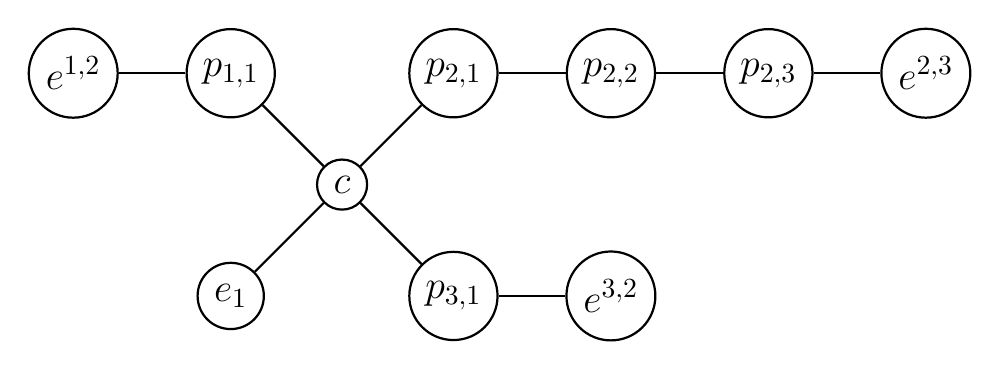
\begin{tikzpicture}[-,auto,node distance=2cm,
                    thick,main node/.style={circle,draw,font=\sffamily\Large\bfseries}]

  \node[main node] (1) {$c$};
  \node[main node] (2) [below left of=1] {$e_{1}$};
  \node[main node] (3) [below right of=1] {$p_{3,1}$};
  \node[main node] (4) [above left of=1] {$p_{1,1}$};
  \node[main node] (5) [above right of=1] {$p_{2,1}$};
  \node[main node] (6) [right of=5]  {$p_{2,2}$};
  \node[main node] (7) [right of=6]  {$p_{2,3}$};
  \node[main node] (8) [right of=7]  {$e^{2,3}$};
  \node[main node] (9) [left of=4] {$e^{1,2}$};
  \node[main node] (10) [right of=3] {$e^{3,2}$};
  
  \path[every node/.style={font=\sffamily}]
    (1) edge  (2)
    edge(3)
    edge(4)
    edge(5)
    (5) edge (6)
    (6) edge (7)
    (7) edge (8)
    (9) edge (4)
    (10) edge (3);
    
\end{tikzpicture}
\end{center}
\caption{Labelling of $S^{1,3,1}_{4}$}
\end{myfigure}

The relabelling of nodes is such that 'elongations' can be identified by its position in the vector and the value of that position. $p_{i,j}$ is the 'penultimate' node of the $i^{th}$ elongation and is currently $j$ distance from the centre($j=0,...,n-1$) and $e^{i,k_{i}}$ is similar the end of the $i^{th}$ elongation, which is $k_{i}+1$ distance from the centre. Any unaffected external nodes are labelled $e_{i}$ for $i=1,...,n-h$.

For ease of notation we will define $ |k| \equiv \sum\limits_{i=0}^{i=h} k_{i}$ and $ k_{\max} \equiv \max\limits_{i=1,2,..,h} k_{i}$

\begin{definition}[General star graph]
The \textit{General star graph}, $S^{\bm{k}}_{n}$ ($\bm{k} \in \mathbb{N}^{h}$) is made from $S_{n}$, by performing subdivision on $h$ of the  initial edges each repeated $k_{i}$ for $i=1,...,h$ . 
\end{definition}

Note. For ease of notation we will use the above format, but will understand that using $k_{i}=0$ is a valid construction, so we can image that $\bm{k} \in \mathbb{N}^n$


\subsection{Basic Analysis}
To start our analysis of this graph, we will look at an expanded graph which can be simplified down to our general star graph. Consider the cyclic graph $C_{2(n+|k|)}$ , we can simplify this graph by node identification to $S^{\bm{k}}_{n}$. The identification mapping is harder to visual from a cycle graph.

For ease of understanding look at an example as in Figure \ref{myfigure: Example of simplification to general star graph}

The mapping is done as such:
\begin{itemize}
\item The centre is identified form nodes $1,1+2(k_{1}+1),1+2(\sum\limits_{i=1}^{2} (k_{i}+1)),...,1+2(\sum\limits_{i=1}^{h}(k_{i}+1),1+2(|k|+h)+2),...,1+2(|k|+h)+2(n-h)$

\item The first branch is identified from the nodes between $2$ and $2(k_{1}+1)$ (Inclusive). $n_{1,i}$ for $i=1,...,k_{1}$ are identified by the two nodes $i+1$ and $2k_{1}+3-i$ , the node $n_{1,k_{1}+1}$ is identified by the one node $k_{1}+2$.

\item The $j$\textsuperscript{th} branch is identified from nodes between $2(\sum\limits_{i=1}^{j-1} (k_{i}+1)))$ and $2(\sum\limits_{i=1}^{j} (k_{i}+1)))$ (Inclusive). $n_{j,i}$ for $i=1,....,k_{j}$ are identified by the two nodes $2(\sum\limits_{i=1}^{j-1} (k_{i}+1)))+(i-1)$ and $2(\sum\limits_{i=1}^{j} (k_{i}+1)))-(i-1)$ , the node $n_{j,k_{j}+1}$ is identified by the one node $2(\sum\limits_{i=1}^{j-1} (k_{i}+1)))+k_{j}$.
\end{itemize}

This mapping gives rise to the general Oscillation

\begin{definition}[General Random Oscillation]
The \textit{oscillation} on $S^{\bm{k}}_{n}$ is any embedded Hamiltonian patrol on $C_{2(n+|k|)}$ under the simplification above. The \textit{random oscillation} on $S^{\bm{k}}_{n}$ is the embedded random Hamiltonian patrol on $C_{2(n+|k|)}$ under the simplification above.
\end{definition}

\begin{lemma}
For $m < 2(n+|k|)$ following the random oscillation
$$V(S^{\bm{k}}_{n}) \geq V(C_{2(n+|k|)})=\frac{m}{2(n+|k|)}$$
and if $m \geq 2(n+|k|)$ then $V(S^{\bm{k}}_{n})=1$, achieved by any oscillation. 
\end{lemma}


\begin{myfigure}
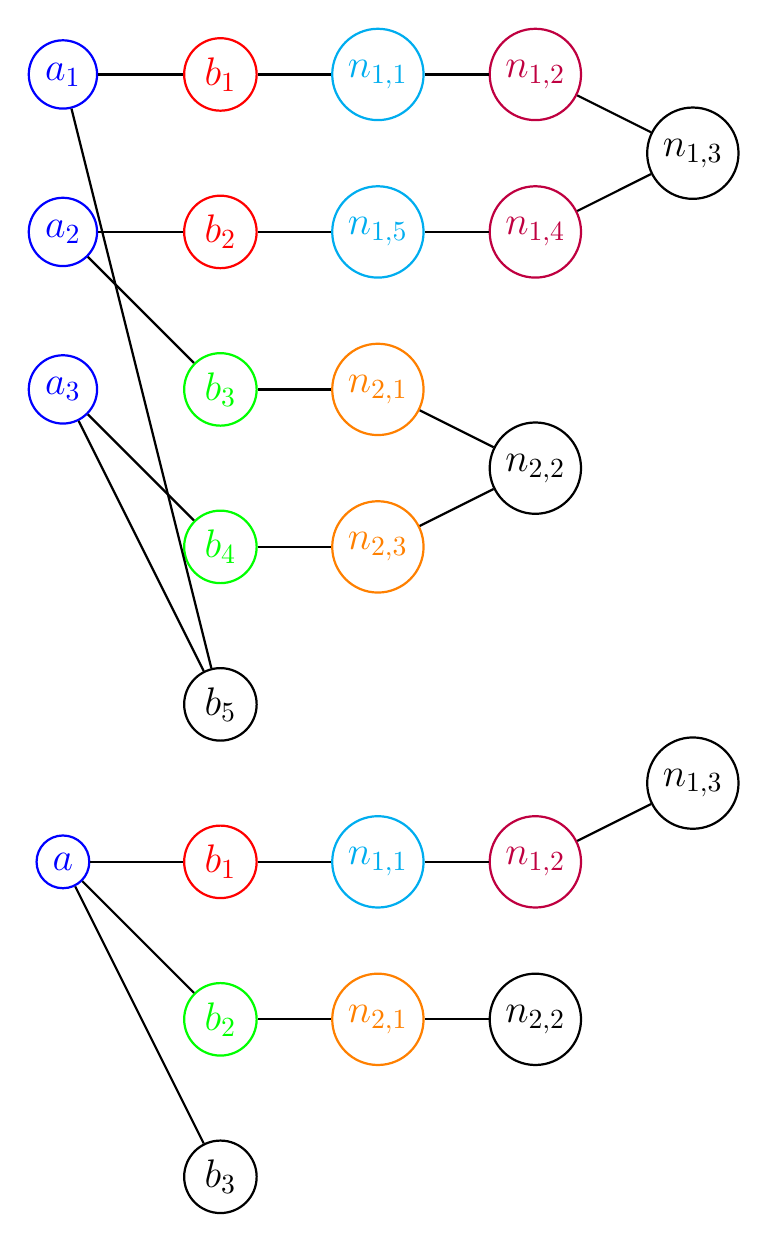
\begin{tikzpicture}[-,auto,node distance=2cm,
                    thick,main node/.style={circle,draw,font=\sffamily\Large\bfseries}]

  \node[main node,color=blue] (1) {$a_{1}$};
  \node[main node,color=blue] (2) [below of=1] {$a_{2}$};
  \node[main node,color=blue] (3) [below of=2] {$a_{3}$};
  \node[main node,color=red] (4) [right of=1] {$b_{1}$};
  \node[main node,color=red] (5) [right of=2]  {$b_{2}$};
  \node[main node,color=green] (6) [right of=3]  {$b_{3}$};
  \node[main node,color=green] (7) [below of=6]  {$b_{4}$};
  \node[main node] (13) [below of=7] {$b_{5}$};
  \node[main node,color=cyan] (8) [right of=4]  {$n_{1,1}$};
  \node[main node,color=purple] (9) [right of=8]  {$n_{1,2}$};
  \node[main node,color=cyan] (10) [right of=5]  {$n_{1,5}$};
  \node[main node,color=purple] (11) [right of=10]  {$n_{1,4}$};
  \node[main node] at (8,-1) (12)  {$n_{1,3}$};
  \node[main node,color=orange] (14) [right of=6] {$n_{2,1}$};
  \node[main node,color=orange] (15) [right of=7] {$n_{2,3}$};
  \node[main node] at (6,-5) (16) {$n_{2,2}$};

  \path[every node/.style={font=\sffamily}]
    (1) edge  (4)
    (2) edge  (5)
        edge  (6)
    (3) edge  (7)
    
    (4) edge (8)
    (13) edge (3)
    (13) edge (1)
    (8) edge (9)
    (9) edge (12)
    (12) edge (11)
    (11) edge (10)
    (10) edge (5)
    (6) edge (14)
    (7) edge (15)
    (14) edge (16)
    (15) edge (16);
  
  \node[main node,color=blue] (13) [below of=3,node distance=6cm] {$a$};
  \node[main node,color=red] (14) [right of=13] {$b_{1}$};
  \node[main node,color=green] (15) [below of=14] {$b_{2}$};
  \node[main node] (16) [below of=15] {$b_{3}$};
  \node[main node,color=cyan] (17) [right of=14] {$n_{1,1}$};
  \node[main node,color=purple] (18) [right of=17] {$n_{1,2}$};
  \node[main node] at (8,-9) (19) {$n_{1,3}$};      
  \node[main node,color=orange] (20) [right of=15] {$n_{2,1}$};
  \node[main node] (21) [right of=20] {$n_{2,2}$}; 
   
   \path[every node/.style={font=\sffamily}]
   (13) edge (14)
   edge (15)
   edge (16)
   (14) edge (17)
   (17) edge (18)
   (18) edge (19)
   (15) edge (20)
   (20) edge (21);
  
\end{tikzpicture}
\caption{Simplification of $C_{16}$ to $S^{3,2}_{3}$}
\label{myfigure: Example of simplification to general star graph}
\end{myfigure}


\begin{myfigure}

\end{myfigure} 

\subsection{solution for $m \geq 2(k_{max}+1)$}
We will match the oscillation bound of $\frac{m}{2(n+|k|)}$, by further extending time-limited attack and time-delayed attack into the type-delayed attack.

\begin{definition}[Node types]
A \textit{type} $i$ node, is an external node which has been extended $i$ times. Let $k_{max} \equiv \max\limits_{i=1,...,h} k_{i}$ be the maximum node type on the general extended star graph, $S_{n}^{\bm{k}}$.
\end{definition}

\begin{definition}[Type-delayed attack]
Let  the \textit{Type-delayed attack}, be the attack that attacks at a type $i$ node with probability $\frac{i+1}{\denominator}$ $\forall \, i$. Choosing an attack interval $I$, the attack at a type $i$ node chooses a interval from the following with equal probability: $I+(k_{max}-i),I+(k_{max}-i)+1,...,I+k_{max}+i+1$ $\forall \, i$ (i.e statring attacks at a type $i$ node at times $\tau+(k_{max}-i)+1,...,\tau+(k_{max}+i)+1$).
\end{definition}

\begin{myfigure}
\begin{center}
\begin{tikzpicture}
 %Drawing Bottom Axis
 \draw[->] (-7,0) -- (7,0);
 \node (timelabel) [shift={(0.2,0)}] at (7,0) {$t$};
 
 
 \draw (-6.5,0.2) -- (-6.5,-0.2);
 \draw (6.5,0.2) -- (6.5,-0.2);
 
 \node (labelc1) at (-6.5,-0.5) {$\tau$};
 \node (labelc2) at (6.5,-0.5) {$\tau+2k_{max}+1$};
 
 \node[cross=5pt,red] (c1) at (-6.5,0.5) {};
 \node[cross=5pt,red] (c2) at (6.5,0.5) {};
 \draw[dashed] (c1) -- (c2);
 \node (linelabel1) at (-8,0.5) {Type $k_{max}$};
 
 
  \draw (-6,0.2) -- (-6,-0.2);
 \draw (6,0.2) -- (6,-0.2);
 
 %\node (labelc1) at (-5.5,-0.5) {$\tau+1$};
 %\node (labelc2) at (5.5,-0.5) {$\tau+2k_{max}-1$};
 
 \node[cross=5pt,red] (c1) at (-6,1.5) {};
 \node[cross=5pt,red] (c2) at (6,1.5) {};
 \draw[dashed] (c1) -- (c2);
 \node (linelabel1) at (-7.5,1.5) {Type $k_{max}-1$};
 
 
 
 \draw[decorate sep={2mm}{4mm},fill] (0,3.5) -- (0,2);

  \draw (-1.5,0.2) -- (-1.5,-0.2);
 \draw (1.5,0.2) -- (1.5,-0.2);
 
 %\node (labelc1) at (-5.5,-0.5) {$\tau+1$};
 %\node (labelc2) at (5.5,-0.5) {$\tau+2k_{max}-1$};
 
 \node[cross=5pt,red] (c1) at (-1.5,4) {};
 \node[cross=5pt,red] (c2) at (1.5,4) {};
 \draw[dashed] (c1) -- (c2);
 \node (linelabel1) at (-2.3,4) {Type $1$};
 
 \draw (-1,0.2) -- (-1,-0.2);
 \draw (1,0.2) -- (1,-0.2);
 
  \node (labelc3) at (-1,-0.5) {$\tau+k_{max}$};
 \node (labelc4) at (1,-0.5) {$\tau+k_{max}+1$};
 
 \node[cross=5pt,red] (c3) at (-1,5) {};
 \node[cross=5pt,red] (c4) at (1,5) {};
 \draw[dashed] (c3) -- (c4);
 \node (linelabel1) at (-1.9,5) {Type $0$}; 

\end{tikzpicture}
\end{center}
\end{myfigure}

\begin{theorem}
When $T \geq m+2k_{max}$, the analogous `diametric' bound is given by
$$V(S_{n}^{\bm{k}}) \leq \max \left\{ \frac{k_{max}+1}{\denominator} , \frac{m}{2 \left( \denominator \right)} \right\}$$
\end{theorem}

Proof: \ref{Type-deayed attack proof}


\begin{corollary}[Solution in $m \geq 2(k_{max}+1)$]
By the attack using the type-delayed attack and the patroller using the random oscillation we achieve the value, when $2(k_{max}+1) \leq m \leq 2(n+|k|)$,
$$V= \frac{m}{2(n+|k|)} $$
and when $m > 2(n+|k|)$ then $V=1$.
\end{corollary}

\section{Dual star graphs}

\section{Linked Star graphs}


%%%%%%%%%%%%%%%%%%%%%
%End of main part of document
\bibliography{mybib}

%%%%%%%%%%%%%%%%%%%%%%%%
\newpage
\appendix
\pagenumbering{roman}
\appendixpage
\addappheadtotoc
\section{Graph Definitions}

\begin{definition}[Graph]
A \textit{graph}, $G=G(N,E)$, is made up of: a set of \textit{nodes} (also called \textit{vertices} or \textit{points}), $N$, which are places ; and a set of \textit{edges} (also called \textit{arcs} or lines), $E$, which are connections between places, so elements of $E$ must be two-element subsets of $N$.
\end{definition}


\begin{definition}[Subgraph]
A graph $Q'=(N',E')$ is said to be a \textit{subgraph} of $Q=(N,E)$ if $N' \subset N$ and $E' \subset E$.

A subgraph is said to be \textit{induced} by $N'$ (or \textit{edge-preserving}) if $E'$ contains all edges (from $E$) that have both end points in $N'$.
\end{definition}


\begin{myfigure}
\begin{center}
\begin{submyfigure}{.3\textwidth}
\begin{center}
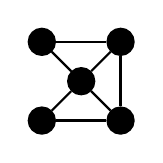
\begin{tikzpicture}[baseline=(current bounding box.north),-,auto,node distance=1cm,
                    thick,main node/.style={circle,draw,fill,font=\sffamily\bfseries}]

  \node[main node] (1) {};
  \node[main node] (2) [right of=1] {};
  \node[main node] (3) [shift={(0.5,-0.5)}] at (1) {};
  \node[main node] (4) [below of=1] {};
  \node[main node] (5) [below of=2] {};
  

  \path[every node/.style={font=\sffamily}]
    (1) edge  (2)
        edge  (3)
    (2) edge  (3)
        edge  (5)
    (4) edge  (3)
        edge  (5)
    (5) edge  (3);
                        
\end{tikzpicture}
\end{center}
\caption{$Q$}
\label{subexamplefigure: before subgraphs}
\end{submyfigure}
\begin{submyfigure}{.3\textwidth}
\begin{center}
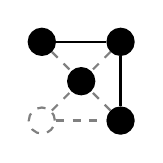
\begin{tikzpicture}[baseline=(current bounding box.north),-,auto,node distance=1cm,
                    thick,main node/.style={circle,draw,fill,font=\sffamily\bfseries}, alt node/.style={circle,draw,dashed,gray,font=\sffamily\bfseries}]

  \node[main node] (1) {};
  \node[main node] (2) [right of=1] {};
  \node[main node] (3) [shift={(0.5,-0.5)}] at (1) {};
  \node[alt node] (4) [below of=1] {};
  \node[main node] (5) [below of=2] {};
  

  \path[every node/.style={font=\sffamily}]
    (1) edge  (2)
    (2) edge  (5);
    
  \path[dashed,gray,font=\sffamily]
    (1) edge (3)
    (2) edge (3)
    (4) edge (3)
        edge (5)
    (5) edge (3);          
                        
\end{tikzpicture}
\end{center}
\caption{$Q_{1}$}
\label{subexamplefigure: subgraph}
\end{submyfigure}
\begin{submyfigure}{.3\textwidth}
\begin{center}
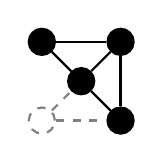
\begin{tikzpicture}[baseline=(current bounding box.north),-,auto,node distance=1cm,
                    thick,main node/.style={circle,draw,fill,font=\sffamily\bfseries}, alt node/.style={circle,draw,dashed,gray,font=\sffamily\bfseries}]

  \node[main node] (1) {};
  \node[main node] (2) [right of=1] {};
  \node[main node] (3) [shift={(0.5,-0.5)}] at (1) {};
  \node[alt node] (4) [below of=1] {};
  \node[main node] (5) [below of=2] {};
  

  \path[every node/.style={font=\sffamily}]
    (1) edge  (2)
    (2) edge  (5)
    (1) edge (3)
    (2) edge (3)
    (5) edge (3);
    
  \path[dashed,gray,font=\sffamily]
    (4) edge (3)
        edge (5);          
                        
\end{tikzpicture}
\end{center}
\caption{$Q_{1}$}
\label{subexamplefigure: induced subgraph}
\end{submyfigure}
\caption{ $Q_{1}$ is a subgraph of $Q$. However it is not induced as it is missing possible edges connecting nodes that existed in $Q$. $Q_{2}$ shows the induced subgraph on the chosen set of nodes. }
\end{center}
\label{examplefigure: subgraph example}
\end{myfigure}

\begin{definition}[Walk,Path,Trail,Cycle]
A sequence of nodes $(n_{0},n_{1},...,n_{l})$ is a \textit{walk} of length $l$ if $e_{n_{i},n_{i+1}} \in E$ $\forall i=0,...,l-1$. Corresponding to a walk is the sequnece of $l$ edges $(e_{n_{0},n_{1}},e_{n_{1},n_{2}},...,e_{n_{l-1},n_{l}})$.

A walk becomes a trail if each edge in the walk is distinct, i.e $e_{n_{i},n_{i+1}} \neq e_{n_{j},n_{j+1}} \forall i \neq j$. A trail becomes a path if each node in the walk is distinct (except possibly the start and final node), i.e $n_{i} \neq n_{j} \forall i \forall i < j \geq l-1$.

A walk,trail or path is said to be \textit{closed} if the start and end nodes are the same. A \textit{cycle} is a closed path with length, $l \geq 3$ (with the special case of $l=3$ being called a \textit{triangle}).
\end{definition}

\begin{definition}[Hamiltonian cycle]
A \textit{Hamiltonian cycle} is a cycle which contains every node on the graph, i.e it is a cycle of length $l=|N|$. A graph that exhibits a Hamiltonian cycle is called \textit{Hamiltonian}
\end{definition}

\begin{figure}
\begin{center}
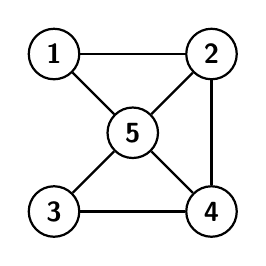
\begin{tikzpicture}[baseline=(current bounding box.north),-,auto,node distance=2cm,
                    thick,main node/.style={circle,draw,font=\sffamily\bfseries}]

  \node[main node] (1) {1};
  \node[main node] (2) [right of=1] {2};
  \node[main node] (3) [shift={(1,-1)}] at (1) {5};
  \node[main node] (4) [below of=1] {3};
  \node[main node] (5) [below of=2] {4};
  

  \path[every node/.style={font=\sffamily}]
    (1) edge  (2)
        edge  (3)
    (2) edge  (3)
        edge  (5)
    (4) edge  (3)
        edge  (5)
    (5) edge  (3);
                        
\end{tikzpicture}
\end{center}
\caption{Graph, $Q$}
\label{figure: walks on graph Q}
\end{figure}

\begin{example}
For the graph $Q$ as in Figure \ref{figure: walks on graph Q}:
\begin{itemize}
\item An example of a walk is $(1,2,1,5,4,2)$
\item An example of a trail is $(1,2,5,3,4,5,1)$
\item An example of a path is $(1,2,4,3)$
\item An example of a Hamiltonian cycle is $(1,2,4,3,5,1)$
\end{itemize}
Hence we would call the graph $Q$ Hamiltonian.
\end{example}

\begin{definition}[Complete graphs]
The \textit{complete graph}, $K_{n}$, is a graph of $n$ nodes, in which all edges are present, i.e $e_{i,i'} \in E \; \forall i,i' \in N$.
\end{definition}

\begin{myfigure}
\begin{center}
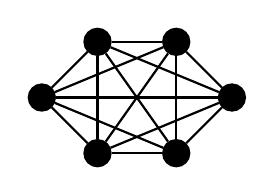
\begin{tikzpicture}[baseline=(current bounding box.north),-,auto,node distance=1cm,
                    thick,main node/.style={circle,fill,draw,font=\sffamily\bfseries}]

  \node[main node] (1) {};
  \node[main node] (2) [right of=1] {};
  \node[main node] (3) [below left of=1] {};
  \node[main node] (4) [below right of=2] {};
  \node[main node] (5) [below right of=3] {};
  \node[main node] (6) [below left of=4] {};
  

  \path[every node/.style={font=\sffamily}]
    (1) edge  (2)
        edge  (3)
        edge  (4)
        edge  (5)
        edge  (6)
    (2) 
        edge  (3)
        edge  (4)
        edge  (5)
        edge  (6)
    (3) 
        edge  (4)
        edge  (5)
        edge  (6)
    (4) edge  (5)
        edge  (6)
    (5) edge  (6);        
                     
\end{tikzpicture}
\caption{The complete graph of $6$ nodes,$K_{6}$.}
\end{center}
\end{myfigure}

\begin{definition}[Bipartite]
A graph is said to be \textit{bipartite} if $N=A \cup B$, where $A \cap B= \emptyset$ ,and $e_{i,i'} \notin E \, \forall i,i' \in A$, $e_{i,i'} \notin E \, \forall i,i' \in B$.
\end{definition}

\begin{definition}[Complete bipartite]
The \textit{complete biparite graph}, $K_{a,b}$, is a bipartite graph of $a+b$ nodes (where $|A|=a$,$|B|=b$), in which all edges are present, i.e $e_{i,i'} \in E \; \forall i \in A \, \forall i' \in B$ and $e_{i,i'} \in E \; \forall i \in B \, \forall i' \in A$.
\end{definition}

\begin{myfigure}
\begin{center}
\begin{submyfigure}{.45\textwidth}
\begin{center}
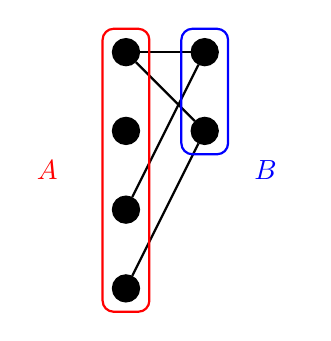
\begin{tikzpicture}[baseline=(current bounding box.north),-,auto,node distance=1cm,
                    thick,main node/.style={circle,draw,fill,font=\sffamily\bfseries}]

  \node[main node] (1) {};
  \node[main node] (2) [below of=1] {};
  \node[main node] (3) [below of=2] {};
  \node[main node] (4) [below of=3] {};
  \node[main node] (5) [right of=1] {};
  \node[main node] (6) [below of=5] {};
  

  \path[every node/.style={font=\sffamily}]
    (1) edge  (5)
        edge  (6)
    (3) edge  (5)
    (4) edge  (6);
        
  \node (ABox) [draw,rounded corners,red, fit= (1) (2) (3) (4)] {};
  \node (BBox) [draw,rounded corners,blue, fit= (5) (6)] {};
  
  \node [left=0.5cm,text width=0.5cm,red] at (ABox) {$A$};
  \node [right=1.5cm,text width=0.5cm,blue] at (ABox) {$B$};              
                     
\end{tikzpicture}
\end{center}
\caption{$Q$}
\label{subfigure: bipartite Q}
\end{submyfigure}
\begin{submyfigure}{.45\textwidth}
\begin{center}
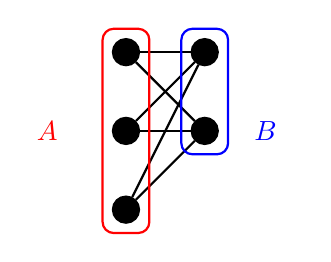
\begin{tikzpicture}[baseline=(current bounding box.north),-,auto,node distance=1cm,
                    thick,main node/.style={circle,draw,fill,font=\sffamily\bfseries}]

  \node[main node] (1) {};
  \node[main node] (2) [below of=1] {};
  \node[main node] (3) [below of=2] {};
  \node[main node] (4) [right of=1] {};
  \node[main node] (5) [below of=4] {};
  

  \path[every node/.style={font=\sffamily}]
    (1) edge  (4)
        edge  (5)
    (2) edge  (4)
        edge  (5)
    (3) edge  (4)
        edge  (5);
        
  \node (ABox) [draw,rounded corners,red, fit= (1) (2) (3)] {};
  \node (BBox) [draw,rounded corners,blue, fit= (4) (5)] {};
  
  \node [left=0.5cm,text width=0.5cm,red] at (ABox) {$A$};
  \node [right=1.5cm,text width=0.5cm,blue] at (ABox) {$B$};              
                     
\end{tikzpicture}
\end{center}
\caption{$K_{3,2}$}
\label{subfigure: complete bipartite}
\end{submyfigure}
\caption{ \ref{subfigure: bipartite Q} is an example of a bipartite graph, Q. \ref{subfigure: complete bipartite} is the complete bipartite graph with set sizes of $3$ and $2$.}
\end{center}
\end{myfigure}

\begin{definition}[Subdivision,Smoothing]
A \textit{Subdivision} (or \textit{expansion}) of a graph, $G$, is a new graph $G'$ which is made by subdividing a chosen edge. The subdivision of an edge $\{u,v\}$ yields a graph with a new node $w$ and the splitting of the edge $\{u,v\}$ into $\{u,w\}$ and $\{w,v\}$.

The reverse process is called \textit{Smoothing} of a graph, $G$, is a new graph $G'$ which is made by smoothing between two nodes. The smoothing out of a node pair $(u,v)$, with $d(u,v)=2$ and with $w$ between them, then $w$ is removed along with the edges $\{u,w\}$ and $\{v,w\}$, then the edge $\{u,v\}$ is placed to connect $u$ and $v$. 
\end{definition}

\begin{myfigure}
\begin{center}
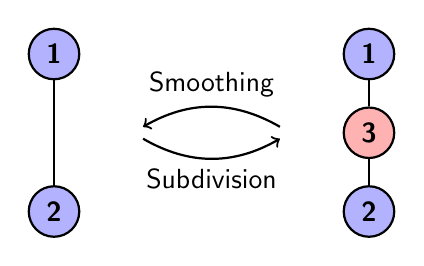
\begin{tikzpicture}[baseline=(current bounding box.north),-,auto,node distance=2cm,
                    thick,main node/.style={circle,draw,font=\sffamily\bfseries}]

  \node[main node,fill=blue!30] (1) {1};
  \node[main node,fill=blue!30] (2) [below of=1] {2};
  

  \path[every node/.style={font=\sffamily}]
    (1) edge  (2);
    
  \node (AP1) [shift={(1,-1)}] {};
  \node (AP2) [shift={(3,-1)}] {};
  
  \path[->,bend right,every node/.style={font=\sffamily}]
    (AP1) edge node[below] {Subdivision} (AP2)
    (AP2) edge node[above] {Smoothing} (AP1);
      
  
  \node[main node,fill=blue!30] (3) [shift={(4,0)}]{1};
  \node[main node,fill=red!30] (4) [shift={(4,-1)}]{3};
  \node[main node,fill=blue!30] (5) [shift={(4,-2)}]{2};
  
  \path[every node/.style={font=\sffamily}]
    (3) edge  (4)
    (4) edge  (5);
  
    
                        
\end{tikzpicture}
\caption{Subdivision and Smoothing of the edge $\{1,2\}$}
\end{center}
\end{myfigure}

\section{Old Statements about Old diametric}
Ignoring the problem with the old diametric bound, the diametric idea from \citep{Alpern2011} can be extended when their are multiple diametric pairs. 

\begin{definition}[Diametrical set]
Let $D=\{ i \in N \, | \, d(i,i')=\bar{d} \quad \forall i' \in D \}$
\end{definition}

\begin{lemma}
By the attacker playing equally likely all nodes in $D$, at a random time interval, called the extended diametric attack gives $V \leq \max\left\{\frac{m}{\raisebox{-0.5ex}{$\scriptstyle |D| \bar{d}$}} , \frac{1}{|D|} \right\}$
\end{lemma}

\begin{proof}
The options for the patroller are to wait at a node and have probability $\frac{1}{|D|}$ or to move between a selection of these nodes and then wait(for some time) or move on. 

The comparison of $m$ to $\bar{d}$ is important (if $m \leq \bar{d}$ waiting at any given node is good), moving is only beneficial if more attacks can be intercepted by moving rather than waiting that is that $m > \bar{d}$ , as this means moving to another node claims $m$ attacks each time compared to waiting which would just give the $\bar{d}$(as this is the time to move), so in this case moving is always better than waiting.

When moving, moving to a the node visited the furtherest in the best will give us the best chance of no-overlap, hence a cycle is formed.

So forming a cycle between the $|D|$ nodes each a distance $\bar{d}$ apart means the probability of intercepting is $\frac{m}{\raisebox{-0.3ex}{$\scriptstyle |D| \bar{d}$}}$.

\end{proof}

\begin{example}
For $S$ as seen in Figure \ref{fig: S}. By the attacker attacking with equal probability on the diametric set of the four 3 nodes, which have $\bar{d}=4$. This gives that $V \leq \max \{ \frac{m}{4 \times 4} , \frac{1}{4} \}= \max \{ \frac{m}{16} , \frac{1}{4}  \}$.

By its simplification from $C_{16}$ , we can get that $V \geq \frac{m}{16}$.

Hence in the region of $m \geq 4$ we get that $V=\frac{m}{16}$
\end{example}

\begin{myfigure}
\begin{center}
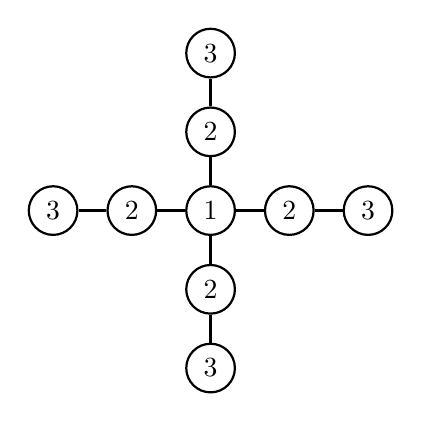
\begin{tikzpicture}[baseline=(current bounding box.north),-,auto,node distance=1cm,
                    thick,main node/.style={circle,draw,font=\sffamily\bfseries}]

  \node[main node] (1) {$1$};
  \node[main node] (2) [right of=1] {$2$};
  \node[main node] (3) [right of=2] {$3$};
  \node[main node] (4) [below of=1] {$2$};
  \node[main node] (5) [below of=4] {$3$};
  \node[main node] (6) [left of=1] {$2$};
  \node[main node] (7) [left of=6] {$3$};
  \node[main node] (8) [above of=1] {$2$};
  \node[main node] (9) [above of=8] {$3$};
  
  \path[every node/.style={font=\sffamily}]
    (1) edge  (2)
    edge (4)
    edge (6)
    edge (8)
    (2) edge (3)
    (4) edge (5)
    (6) edge (7)
    (8) edge (9);
  
\end{tikzpicture}
\end{center}
\caption{Graph $S$ used in example}
\label{fig: S}
\end{myfigure}


\section{Improvemening Hamiltonian bound}

\subsection{Reason For Probability of Interception formula}
\label{appednixsection: Reason for probability of interception}
To argue why this is consider looking at just the integer points on the graph first,
then by looking whether it is best to return via the ``left return'' or a ``right return'', that is the shortest time to the next return along the oscillation. The time/distance to return via the left motion, i.e through $1$, is $2(i-1)$ and the time/distance to return via the right motion, i.e through $c$ and the set of $*$'s, is $2(n+k-(i-1))=2(n+k+1-i)$. So the categories fall when $2(i-1) < 2(n+k+i-1) , 2(i-1)=2(n+k+1-i) , \text{ and } 2(i-1) > 2(n+k+1-i)$. These decide the boundaries and they return with these distances.

Therefore the patroller catches the $m$ initially and then either another $t$ or $m$ attacks on the return, where $t$ is the time to next return (either $2(i-1)$ or $2(n+k+1-i)$). This means that the patroller catches $\min(m+t,2m)$ attacks and hence the probability of interception is $\frac{\min(m+t,2m)}{2(n+k)}$ as they cycle is of length $2(n+k)$ and the number lies in $\min(m+t,2m)$ of these.

For $c$ consider that it catches $m$ attacks initially and is returned to $n-1$ times each at a distance/time of $2$ apart, meaning it gains $t=2$ or $m$ attacks $n-1$ attacks. Hence it intercepts $\min(m+2(n-1),nm)$ out the cycle length of $2(n+k)$.

Finally $*$ nodes are easy as they are they are not returned to in a single cycle, hence they intersect $m$ out the possible $2(n+k)$.

\subsection{Naive Improvement Complete analysis}
\label{appendix:Naiveanalysis}
\begin{enumerate}
\item If $M= \emptyset, R= \emptyset$ then $C_{min} (\alpha)=\min \{ C_{min}^{L} , C_{min}^{S} \}=\min \{ Pw(1)+q_{L} , Pw(*)+q_{S} \}=P\frac{m}{2(n+k)} + \min \{ q_{L}, q_{S} \}$. As the Patroller wishes to select $q_{L},q_{S}$ to maximize this probability, the problem becomes 
$$\begin{array}{cc}
\text{Maximize} &(1-q_{L}-(n-1)q_{S}) \frac{m}{2(n+k)}+\min \{ q_{L}, q_{S}  \} \\
\text{Subject to } & q_{L}+(n-1)q_{S} \leq 1 \text{  (Probability sum constraint)} \\
     & q_{L},q_{S} \geq 0 \\
\end{array} $$
Meaning that as due to the symmetry of $q_{L},q_{S}$ we must have that $q_{L}=q_{S}$ which means improvement is only possible if $2(n+k)-nm \geq 0$ , then set $q_{L}=q_{S}=\frac{1}{n}$. Meaning $P=0,Q_{L}=\frac{1}{n},Q_{R}=\frac{n-1}{n}$ and giving a lower bound $V \geq \frac{1}{n}$.

\item If $M \neq \emptyset,R=\emptyset$ then $C_{min} (\alpha)=\min \{ C_{min}^{L} ,C_{min}^{M}, C_{min}^{S} \}=\min \{ Pw(1)+q_{L} ,Pw(\floor{\frac{m}{2}+2}), Pw(*)+q_{S} \}=P\frac{m}{2(n+k)} + \min \{ q_{L}, P \frac{m}{2(n+k)} , q_{S} \}$. As the Patroller wishes to select $q_{L},q_{S}$ to maximize this probability, the problem becomes
$$\begin{array}{cc}
\text{Maximize} &(1-q_{L}-q_{S}) \frac{m}{2(n+k)}+\min \{ q_{L},(1-q_{L}-(n-1)q_{S})\frac{m}{2(n+k)}, q_{S}  \} \\
\text{Subject to } & q_{L}+(n-1)q_{S} \leq 1 \text{  (Probability sum constraint)} \\
     & q_{L},q_{S} \geq 0 \\
\end{array} $$ 
Meaning that as due to the symmetry of $q_{L},q_{S}$ we must have that $q_{L}=q_{S}$, with improvement only possible if $2(n+k)-nm \geq 0$ , which means we seek to maximize $(1-nq_{L}) \frac{m}{2(n+k)}+\min \{ q_{L},(1-nq_{L})\frac{m}{2(n+k)} \}$ giving $q_{L}=\frac{m}{2(n+k)+nm}$ (as one is then decreasing in $q_{L}$ and one is increasing in $q_{L}$). Meaning $P=\frac{2(n+k)}{2(n+k)+mn},Q_{L}=\frac{m}{2(n+k)+mn},Q_{S}=\frac{m(n-1)}{2(n+k)+mn}$ and giving a lower bound $V \geq \frac{2m}{2(n+k)+mn}$

\item If $M \neq \emptyset,R \neq \emptyset$ then $C_{min} (\alpha)=\min \{ C_{min}^{L} ,C_{min}^{M}, C_{min}^{R}, C_{min}^{S} \}=\min \{ Pw(1)+q_{L} ,Pw(\floor{\frac{m}{2}+2}), Pw(k+1)+q_{S}, Pw(*)+q_{S} \}=P\frac{m}{2(n+k)} + \min \{ q_{L}, P \frac{m}{2(n+k)} , q_{S} \}$. Now was $Pw(k+1) +q_{S} \geq PW(*)+q_{S}$, we can ignore this element (meaning here it does not matter if $R$ is empty or not).
As the Patroller wishes to select $q_{L},q_{S}$ to maximize this probability, the problem becomes
$$\begin{array}{cc}
\text{Maximize} &(1-q_{L}-(n-1)q_{S}) \frac{m}{2(n+k)}+\min \{ q_{L},(1-q_{L}-(n-1)q_{S})\frac{m}{2(n+k)}, q_{S}  \} \\
\text{Subject to } & q_{L}+(n-1)q_{S} \leq 1 \text{  (Probability sum constraint)} \\
     & q_{L},q_{S} \geq 0 \\
\end{array} $$
Meaning that as due to the symmetry of $q_{L},q_{S}$ we must have that $q_{L}=q_{S}$, with improvement only possible if $2(n+k)-nm \geq 0$ , which means we seek to maximize $(1-nq_{L}) \frac{m}{2(n+k)}+\min \{ q_{L},(1-nq_{L})\frac{m}{2(n+k)} \}$ giving $q_{L}=\frac{m}{2(n+k)+nm}$ (as one is then decreasing in $q_{L}$ and one is increasing in $q_{L}$). Meaning $P=\frac{2(n+k)}{2(n+k)+mn},Q_{L}=\frac{m}{2(n+k)+mn},Q_{S}=\frac{m(n-1)}{2(n+k)+mn}$ and giving a lower bound $V \geq \frac{2m}{2(n+k)+mn}$

\end{enumerate}

\subsection{Combinatorial Improvement Complete analysis}
\label{appendix:Choosinganalysis}
\begin{enumerate}
\item If $M= \emptyset , R= \emptyset$ then $C_{min} (\beta_{2})=\min \{ C_{min}^{L} , C_{min}^{S} \}= \min \{ Pw(1)+q_{L} , Pw(*)+q_{S} \}=P\frac{m}{2(n+k)} + \min \{ q_{L} , q_{S} \} $. As the patroller wishes to select $q_{L},q_{S}$ to maximize this probability the problem becomes
$$\begin{array}{cc}
\text{Maximize} &(1-q_{L}-\frac{n-1}{\floor{\frac{m}{2}}}q_{S}) \frac{m}{2(n+k)}+\min \{ q_{L}, q_{S}  \} \\
\text{Subject to } & q_{L}+\frac{n-1}{\floor{\frac{m}{2}}}q_{S} \leq 1 \text{  (Probability sum constraint)} \\
     & q_{L},q_{S} \geq 0 \\
\end{array} $$
Meaning that due to the symmetry of $q_{L},q_{S}$ we must have that $q_{L}=q_{S}$, which means that improvement is only possible if $2(n+k)- m(1+\frac{n-1}{\floor{\frac{m}{2}}}) \geq 0$. Then setting $q_{L}=q_{S}=\frac{\floor{\frac{m}{2}}}{\floor{\frac{m}{2}} +n-1}$. Meaning $P=0, Q_{L}=\frac{\floor{\frac{m}{2}}}{\floor{\frac{m}{2}} +n-1} , Q_{S}=\frac{n-1}{\floor{\frac{m}{2}} +n-1}$ and giving a lower bound of $V \geq \frac{\floor{\frac{m}{2}}}{\floor{\frac{m}{2}} +n-1}$

\item If $M \neq \emptyset , R= \emptyset$ then $C_{min} (\beta_{2})=\min \{ C_{min}^{L} , C_{min}^{M} , C_{min}^{S} \}=\min \{Pw(1)+q_{L}, Pw(\floor{\frac{m}{2}}+2) , Pw(*)+q_{S} \}=P \frac{m}{2(n+k)} + \min \{q_{L}, P \frac{m}{2(n+k) , q_{S}} $. As the patroller wishes to select $q_{L},q_{S}$ to maximize this probability the problem becomes
$$\begin{array}{cc}
\text{Maximize} & (1-q_{L}-\frac{n-1}{\floor{\frac{m}{2}}}q_{S}) \frac{m}{2(n+k)} + \min \{q_{L}, (1-q_{L}-\frac{n-1}{\floor{\frac{m}{2}}}q_{S}) \frac{m}{2(n+k)} , q_{S} \}\\
\text{Subject to } & q_{L}+\frac{n-1}{\floor{\frac{m}{2}}}q_{S} \leq 1 \text{  (Probability sum constraint)} \\
     & q_{L},q_{S} \geq 0 \\
\end{array} $$
Meaning that due to symmetry of $q_{L},q_{S}$ we must have that $q_{L}=q_{S}$, which means that the improvement is only possible if $2(n+k)- m(1+\frac{n-1}{\floor{\frac{m}{2}}}) \geq 0$. Then setting $q_{L}=q_{S}$ means we must maximize $(1-(1+\frac{n-1}{\floor{\frac{m}{2}}}q_{L}) \frac{m}{2(n+k)} + \min \{q_{L}, 1-(1+\frac{n-1}{\floor{\frac{m}{2}}}q_{L}) \frac{m}{2(n+k)}\}$ giving $q_{L}=\frac{m}{2(n+k)+m(1+\frac{n-1}{\floor{\frac{m}{2}}}}$ (as one is increasing in $q_{L}$ and one is decreasing in $q_{L}$). Meaning $P=\frac{2(n+k)}{2(n+k)+m(1+\frac{n-1}{\floor{\frac{m}{2}}})}, Q_{L}=\frac{m}{2(n+k)+m(1+\frac{n-1}{\floor{\frac{m}{2}}})}, Q_{S}=\frac{m(n-1)}{\floor{\frac{m}{2}}(2(n+k)+m(1+\frac{n-1}{\floor{\frac{m}{2}}}))}$ and giving a lower bound of $V \geq \frac{2m}{2(n+k)+m(1+\frac{n-1}{\floor{\frac{m}{2}}})}$

\item If $M \neq \emptyset , R \neq \emptyset$ then $C_{min} (\beta_{1})=\min \{ C_{min}^{L} , C_{min}^{M} , C_{min}^{R}, C_{min}^{S} \}=\min \{ Pw(1)+q_{L}, Pw(\floor{\frac{m}{2}}+2), Pw(k+1)+q_{S}, Pw(*)+q_{S} \}=\min \{ Pw(1)+q_{L}, Pw(\floor{\frac{m}{2}}+2), Pw(*)+q_{S} \}=P \frac{m}{2(n+k)} + \min \{ q_{L}, P \frac{m}{2(n+k)} , q_{S}  \}$ As $Pw(k+1)+q_{S} \geq Pw(1)+q_{S}$, we can ignore the element (meaning here it does not matter if $R$ is empty or not).As the patroller wishes to select $q_{L},q_{S}$ to maximize this probability the problem becomes
$$\begin{array}{cc}
\text{Maximize} & (1-q_{L}-q_{S}) \frac{m}{2(n+k)} + \min \{ q_{L}, (1-q_{L}-q_{S}) \frac{m}{2(n+k)} , q_{S} \}\\
\text{Subject to } & q_{L}+q_{S} \leq 1 \text{  (Probability sum constraint)} \\
     & q_{L},q_{S} \geq 0 \\
\end{array} $$
Meaning that due to symmetry of $q_{L},q_{S}$ we must have that $q_{L}=q_{S}$, which means that the improvement is only possible if $n+k-m \geq 0$. Then setting $q_{L}=q_{S}$ means we must maximize $(1-2q_{L})\frac{m}{2(n+k)} + \min \{ q_{L} , (1-2q_{L}) \frac{m}{2(n+k)} \}$ giving $q_{L}=\frac{m}{2(n+k+m)}$ (as one is increasing in $q_{L}$ and one is decreasing in $q_{S}$). Meaning $P=\frac{2(n+k)}{2(n+k+m)},Q_{L}=\frac{m}{2(n+k+m)},Q_{S}=\frac{m}{2(n+k+m)}$ and giving a lower bound of $V \geq \frac{2m}{2(n+k+m)}$.
\end{enumerate}

\subsection{Combinatorial loop improvement analysis}
\label{appendix: Combinatorial loop improvement analysis}
We are only dealing with $m$ odd so $m'=m+1$ even and $M \neq \emptyset$ $R = \emptyset$. We will play the hamiltonian bound with probability $P$, the left end-ensuring improvement with probability $q_{L}$ and the a particular right loop with probability $q_{S}$ (so $Q_{S}=\frac{n-1}{\frac{m'}{2}}q_{S}$.

$C_{min}(C_{min}^{L},C_{min}^M,C_{min}^S)=\min\{Pw(1)+q_{L},Pw(\floor{\frac{m}{2}}+2) Pw(*)+\frac{m}{m'}q_{s}\}=P\frac{m}{2(n+k)}+\min\{q_{L},P\frac{m}{2(n+k)},\frac{m}{m'}q_{S} \}$ As the patroller wishes to select $q_{L},q_{S}$ to maximise the probability the problem becomes

$$\begin{array}{cc}
\text{Maximize} & (1-q_{L}-\frac{n-1}{ \frac{m'}{2}}q_{S}) \frac{m}{2(n+k)} + \min \{ q_{L}, (1-q_{L}-\frac{n-1}{\frac{m'}{2}}q_{S}) \frac{m}{2(n+k)} , \frac{m}{m'}q_{S} \}\\
\text{Subject to } & q_{L}+\frac{n-1}{\frac{m'}{2}}q_{S} \leq 1 \text{  (Probability sum constraint)} \\
     & q_{L},q_{S} \geq 0 \\
\end{array} $$

Meaning that we must have $q_{L}=\frac{m}{m'}q_{S}$ which means the improvement is only possible if $m+2(n-1) \leq 2(n+k)$ (for similarity to even normal combinatorial improvement $\iff m(1+\frac{n-1}{\frac{m}{2}}) \leq 2(n+k)$). 

Then setting $q_{L}=\frac{m}{m'}q_{S}$ means we must maximize $(1-\frac{m+2(n-1)}{m}q_{L})\frac{m}{2(n+k)}+\min\{ q_{L}, (1-\frac{m+2(n-1)q_{L}}{m})\frac{m}{2(n+k)} \}$ giving $q_{L}=\frac{m}{2(n+k)+m+2(n-1)}$. Meaning $P=\frac{2(n+k)}{2(n+k)+m+2(n-1)}$ , $Q_{L}=q_{L}=\frac{m}{2(n+k)+m+2(n-1)}$ and $Q_{S}=\frac{n-1}{\frac{m'}{2}}q_{S}=\frac{2(n-1)}{m}q_{L}=\frac{2(n-1)}{2(n+k)+m+2(n-1)}$. Giving a lower bound of $V \geq \frac{2m}{2(n+k)+m+2(n-1)}$

\begin{note}
It is worth noting that this is analogous to the result found by the usual combinatorial improvement when $m$ is even.
\end{note}


\section{Proof's}

\subsection{Alternating Random Hamiltonian proof}
\label{Alternating Random Hamiltonian proof}

\begin{proof}
During any attack interval $I$ which is of even length, then $W(I)$ contains $m'$ ``even'' and $m'$ ``odd'' nodes for a total of $m=2m'$ nodes. Therefore by following the Alternating Random Hamiltonian Patrol, $\pmb{\pi}_{ARHP}$, with probability $p$ at ``even'' nodes and probability $\frac{2}{n}-p$ at ``odd'' nodes. Then

\begin{align*}
&P(\bm{\pi}_{ARHP},[i,I]) \geq \underbrace{\overbrace{p}^{\text{even node}}+\overbrace{\frac{2}{n}-p}^{\text{odd node}}+p+\frac{2}{n}-p+...+p+\frac{2}{n}-p}_{m=2m' \text{ elements}} \\
&=m' p+m'(\frac{2}{n}-p)=\frac{2m'}{n}=\frac{m}{n} \quad \forall i \in N \quad \forall I \subseteq \mathcal{T}
\end{align*}
Hence as it holds for all pure attacks
$$P(\bm{\pi}_{ARHP},\bm{\phi}) \geq \frac{m}{n} \quad \forall \bm{\phi} \in \Phi$$
Hence $V \geq \frac{m}{n}$ .
\end{proof}

If $m$ is odd, say $m=2m'+1$ then in the above we get two possibilities for each node depending on the interval choice either $p+\frac{m-1}{n}$ or $\frac{m+1}{n}-p$. So choosing anything other than $p=\frac{1}{n}$ (which is the Random Hamiltonian Patrol strategy) gives a worse result for the patroller.

\subsection{Condition on T for old diametric proof}
\label{Condition on T for old diametric proof}

\begin{proof}
Using $T=m-1+(k+1)\bar{d}$ in the formula gives,
$\alpha=\floor{\frac{(k+1) \bar{d}-m}{\bar{d}}}=(k+1)+\floor{\frac{-m}{\bar{d}}}=(k+1)-2=(k-1)$ (the final part is because $2>\frac{-m}{\bar{d}} \geq -1$ and we will assume that $m > \bar{d}$ here otherwise waiting at one node is just as good as the bound we are trying to achieve)

$m-\bar{d}+\pospart{m + m(k-1)} + \pospart{m-1-(m-1+(k-1+1)\bar{d})}+\pospart{m-1-(m-1+(k+1)\bar{d})}$

which is $m-\bar{d}+\pospart{mk} + \pospart{(k+1)\bar{d}-k\bar{d}}+\pospart{(k+1)\bar{d}-(k+1)\bar{d}}$
giving $m-\bar{d}+mk+ \pospart{\bar{d}}+\pospart{0}=m(k+1)$.
Giving the fraction of $\frac{m(k+1)}{2(k+1)\bar{d}}=\frac{m}{2 \bar{d}}$.


For the second part, first we seek to prove that within the choice of $T$ from $m-1+(k+1)\bar{d}+r$ where $0 \leq r < \bar{d}$ is the maximum when $r=m$ (i.e $T=2m-1+(k+1)\bar{d}$).

As the choice of $r$ only affects the final 3 parts (middle and ends values), we can just look at considering these values and seeing what the maximal choice is.

Upon substitution we get that:
$\alpha=\floor{\frac{(k+1)\bar{d}+r-m}{\bar{d}}}=(k+1)+\floor{\frac{r-m}{\bar{d}}}$

so formula becomes
$\pospart{m(\alpha+1)}+\pospart{(k+1)\bar{d}+r-(\alpha+1)\bar{d}}+
\pospart{(k+1)\bar{d}+r-(\alpha+2)\bar{d}}$. To decide $r$ we need to know if middle values or end values are non-zero.

Note. The second end value will never be non-zero as $(k+1)\bar{d}+r-(\alpha+2)\bar{d}=(k+1)\bar{d}+r-((k+1)+\floor{\frac{r-m}{\bar{d}}}+2)\bar{d}=r-(\floor{\frac{r-m}{\bar{d}}+2}\bar{d} < r-(-1+2)\bar{d}=r-\bar{d}<0$.

\begin{itemize}
\item No middle values and no end values is impossible assuming $k \in \mathbb{N}_{0}$.

\item Middle values but no end values. As we really want to maximize the end value, increasing $r$ up to the point where $\alpha$ increases (giving a raise of $m$ attacks captured) but increases the number of total attacks by 2 each time it is raised. Hence minimal $r$ is chosen to increase $\alpha$. This is when $r-m=-\bar{d}$ i.e $r=m-\bar{d}$ changes $\alpha$ by 1 (as $r<m-\bar{d}$ gives an -1 to $\alpha$, but critical point is when equal to).

\item Middle values and end value. As we are looking at $(m-\bar{d})(\alpha+1)+(k+1)\bar{d}+r$, we still want to increase $\alpha$ without increasing the number of attacks too much, i.e as above.
\end{itemize}

Then we show that the maximal subsequence tends to the bound as $T \rightarrow \infty$, i.e as $k \rightarrow \infty$.
When substituted, we get that
$\alpha=(k+1)$ and so the formula becomes
$m-\bar{d}+\pospart{m + m(k+2)} + \pospart{2m-1-(m-1+(k+2)\bar{d})}+\pospart{2m-1-(m-1+(k+3)\bar{d})}$
giving $m-\bar{d}+(k+3)m + \pospart{m-(k+2)\bar{d}}+\pospart{m-(k+3)\bar{d}}$.
As $m < 2\bar{d}$ then we get $m(k+4) -\bar{d}$ caught out of $2(m+k\bar{d})$
giving a fraction of $\frac{m(k+4)-\bar{d}}{2(m+k\bar{d}} \rightarrow \frac{m}{2\bar{d}}$.

Hence as the maximal subsequence tends down to the bound, it implies the result.
\end{proof}

\subsection{Time-limited diametric attack proof}
\label{Time-limited diametric attack proof}

\begin{proof}
First consider all the pure patrolling strategies, $W_{i} \in \mathcal{W}$, Then as the attacker is only attacking two ends, henceforth called $n_{1}$ and $n_{\bar{d}}$, any patrol not starting at $n_{1}$ or $n_{\bar{d}}$ is dominated by one that does.
This is because the patrol will not capture any attacks until they visit either $n_{1}$ or $n_{\bar{d}}$, and then capture a set of attacks that started there previously. The patrol might as well wait there up until this point and do at least as good as arriving there for the first time.

Formally, assume that $n_{1}$ is the end node first reached by a patrol, $W(t)$ at time, $t_{1}=\min \set{t}{W(t)=n_{1}}$, then we can form the patrol, $U(t)= \left\{ \begin{array}{l}
n_{1} \text{ for } t \leq t_{1}, \\
W(t) \text{ for } t>t_{1}. \\
\end{array} \right.$
and $P(U,\phi) \geq P(W,\phi)$ where $\phi$ is the timed diametric attack (or infact the normal diametric attack.

Now we are restricted to patrols starting at end points, it is similar to see when leaving an end point, there is no other decision as you must travel to the other end point, assumed to be $n_{\bar{d}}$. Hence the question becomes when to leave $n_{1}$ and travel to $n_{\bar{d}}$. Obviously it should only be undertaken if the journey can be made and more attacks can be caught by doing so.

WLOG assume that $\tau=0$ (other just wait longer initially, as attacks haven't started), then our choice is what leaving time (last time before moving): $t_{l} \in \{0,1,...,m-2 \}$, to pick to maximize the number of attacks caught; or $t_{L}=\infty$, never leaving to get $\bar{d}$ attacks.

\begin{itemize}
\item[Leaving:]Choosing $t_{L} \in \{0,1,...,m-2 \}$ gives the patroller $\frac{m}{2\bar{d}}$ as,

Leaving at $t_{L}$ gives us $\min(t_{L}+1,\bar{d})$ attacks caught at $n_{L}$, and $\min(m+\bar{d}-2-(t_{L}+\bar{d})+1,\bar{d})=\min(m-1-t_{L},\bar{d})$.

Now choosing $t_{L} > \bar{d}-1$, doesn't improve the first value and possibly lowers the second value. Hence we restrict ourselves to leave if we catch all attacks, i.e $t_{L} \leq \bar{d}-1$. Now in this region lowering $t_{L}$ lowers it by $1$ and raises it only raises the second on by $1$ if $m-1-t_{L} \leq \bar{d}$ (i.e $t_{L} \geq m-1-\bar{d}$ or any $t_{L}$ if $m-1-\bar{d} \leq 0$). Hence any choice of $\pospart{m-1-\bar{d}} \leq t_{L} \leq \bar{d}-1$ is equally as good. This gives a number of attacks caught as $t_{L}+1+m-1-t_{L}=m$ out of $2\bar{d}$ placed attacks. Hence giving $V \leq \frac{m}{2\bar{d}}$.

\item[Staying:]Choosing $t_{L}=\infty$ gives the patroller $\frac{1}{2}$
\end{itemize}

Hence as the patroller can pick from these two options, it gives $V \leq \max\{\frac{1}{2} , \frac{m}{2\bar{d}} \}$. More explicity it gives $V \leq \frac{1}{2}$ if $m < \bar{d}$, and $V \leq \frac{m}{2\bar{d}}$ is $m \geq \bar{d}$.
\end{proof}

\subsection{Polygonal attack proof}
\label{Polygonal attack proof}

\begin{proof}
First consider all the pure patrolling startegies, $W_{i} \in \mathcal{W}$, Then we immediately restrict ourselves to pure patrols starting at an attack point, assumed WLOG $n_{1}$ is the first node hit by a patrol. This restriction is possibly as if our current strategy, $W$, doesn't hit $n_{1}$ until time $t_{hit}=\min \set{t}{W(t)=n_{1}}$, then we can form the patrol $U(t)=\left\{ \begin{array}{l} 
n_{1} \text{ for } t \leq t_{hit}, \\
W(t) \text{ for } t > t_{1}. \\
\end{array} \right. $ with $P(U,\phi) \geq P(W,\phi)$, where $\phi$ is the polygonal attack.

Now we are restricted to start at $n_{1}$, and when we leave $n_{1}$ we will not return immediately for a similar reason to the above (as we could form a patrol which waits longer before leaving to do at least as good). So when we leave we can only go to one of the other end points, say WLOG $n_{2}$ (as all end points attacks are equivalent). Similarly from this position we will be waiting until we leave and then head to another end point, which is not yet visited.

Note. We cannot every have a unvisited end point as $m \leq |D|d$ (otherwise the value is $1$) and we will therefore never visit the same node twice.

This means the patroller will be performing a strategy that only chooses when to leave a currently at node. This means a choice among the vector $\mathbf{t}=(t_{1},...,t_{|D|})$ where $t_{i}=\max \set{t}{W(t)=n_{i}}$, with $t_{i}=\infty$ meaning never leave and the vector increasing by at least $d$ for increase in index, i.e $t_{i+1} \geq t_{i}+d$ (and so by induction $t_{i} \geq (i-1)d$).

Now we will suppose that $kd \leq m < (k+1)d$ for some $k \in \{ 0,1,...,|D|-1 \}$, as this will determine the behaviour of the vector $\mathbf{t}$ and assume WLOG that $\tau=0$ (so $I=\{0,1,...,m-1 \}$)

We can first argue that when leaving, if the current time,$t \geq d$ then there is no point waiting for any time at a node. This is because past this time, no more attack at that node are being carried out and hence the maximum number has been caught when arriving at a node. Hence we really only have a decision for the first node $t_{1}$ (as $t_{i} \geq d$ for $i \geq 2$), and this decision will be based on the total number of attacks caught.

Now as $m <(k+1)d$ along our strategy the maximum number of end points we will visit it $(k+1)$.

The formula under this patrol for the number of attacks caught will be
\begin{align*}
&\min(t_{1}+1,d)+\min(m+d-2-(t_{1}+d)+1,d)+\min(m+d-2-(t_{1}+2d)+1,d)+...
+\min(m+d-2-(t_{1}+kd),d)
&=\min(t_{1}+1,d)+\min(m-1-t_{1},d)+\min(m-1-t_{1}-d,d)+...+\min(m-1-t_{1}-(k-1)d,d)
\end{align*}
Note. No negative values are to be summed

As $t_{1}$ is limited to pick $d-1$ or below (as otherwise picking up no additional attacks), we can note that decreases $t_{1}$ the first term decreases, and the second term increases only if $0 \leq m-1-t_{1} \leq d$, i.e $m-1-d \leq t_{1} \leq m-1$.

Now as $m-1-d \geq kd-1-d=(k-1)d-1$ this means that we require that $(k-1)d-1 \leq t_{1} \leq d-1$ meaning unless $k=1$, this will not increase, the value will always be $d$ as $\min(m-1-d,d) \geq \min(kd-1-d,d)=\min((k-1)d-1,d)=d$ (for $k \geq 2$).

Similary the $j$\textsuperscript{th} value, past the first value, has the contribution of $\min(m-1-t_{1}-(j-1)d,d)$ , so for a increase we only get it if $ 0 \leq m-1-t_{1}-(j-1)d \leq d \implies m-1-(j-1)d \geq t_{1} \geq m-1-jd \geq (k-j)d-1$ and as $t_{1} \leq d-1$ it means it will only be increasing if $j=k$ (note. $j=k-1$ gives an acceptable range of $t_{1}$ but does not allow it to decrease in the first place).


So decreasing $t_{1}$ from $d-1$ by $1$ increases the last value by $1$ only if $t_{1} \geq m-1-kd$. However this still provides overall number of attacks caught.
Now note by our 

\begin{align*}
&\min(t_{1}+1,d)+\underbrace{d+d+...+d}_{k-1 \text{ lots of } d}+\min(m-1-t_{1}+(k-1)d,d)
&\min(d-1+1,d)+(k-1)d+\min(m-1-(d-1)-(k-1)d,d)
&=d+(k-2)d+\min(m-kd,d)=d+(k-1)d+m-kd=m
\end{align*}  
As noting $m-kd \geq 0$ by assumption earlier.
This gives $V \leq \frac{m}{|D|d}$

It has already been noted that any choice of $t_{i}$ for $i \geq 2$ should be $t_{i}=t_{i}+(i-1)d$. So there will never be option to use these as $t_{i}=\infty$. However $t_{1}$ could be chosen to be $\infty$, this would give a bound of $V \leq \frac{1}{|D|}$.

Hence the patroller can pick from these two options, giving $V \leq \max \{ \frac{1}{|D|} , \frac{m}{|D|d} \}$. More explicitly it gives $V \leq \frac{1}{|D|}$ if $m < d$ and $V \leq \frac{m}{|D|d}$ if $m \geq d$.
\end{proof}

\subsection{Time-delayed attack proof}
\label{Time-delayed attack proof}
\begin{proof}
First Consider a patrolling strategy that is at a $*$ node at time $t \geq k$ (i.e $*$ node attacks have begun) and seek to show that staying amongst the $*$ nodes until the attacks end is at least as good as moving to node $1$ and waiting, and possibly returning to $*$ (if time allows).

We will consider two cases of $m \leq 2(k+1)$ and $m > 2(k+1)$.
\begin{itemize}
\item[1.] In this case we will first show that returning to $*$ type nodes is never an option once it is left, consider leaving at $t$, then the first possible return would be $t+2(k+2) \geq k + 2(k+2) > k+m$ and hence all the attacks would be caught and there would be no point returning. Hence the only option in this scenario is whether it is worth it leave at this point $t$ and go to node $1$ and wait until the end of the game.

If she was to stay around the end nodes then from this point onwards (not including the node we are at , at time $t$) we would get a payoff of $\frac{k+m-t-1}{2(n+k)}$.

This is becuase we either get:
\begin{itemize}
\item[$k+m$ odd] $\underbrace{\frac{1}{n+k}+...+\frac{1}{n+k}}_{\frac{k+m-t}{2} \text{times}}$
\item[$k+m$ even] $\underbrace{\frac{1}{n+k}+...+\frac{1}{n+k}}_{\frac{k+m-1-t}{2}-1 \text{times}} +\frac{1}{2(n+k)}$
\end{itemize}

In either case the payoff for moving about at the $*$ type nodes is as above.

Now consider moving away to $1$, which will be reached at time $t+k+2$ and as we must wait here the payoff depends on a few things. It is 
$$\frac{\min (m,t+k+2,m-(t+k+2-(2k+1))}{2(k+1)} \times \frac{k+1}{n+k} =
\frac{\min (m,t+k+2,k+m-t-1)}{2(n+k)}$$

now note as $t \geq k \implies m > k+m-t-1$ and as $m \leq 2(k+1) \implies t+k+2 \geq m$. Moreover this implies we will be in the final stretch of attacks and no new attacks will be taking place, so no more attacks will be claimed by waiting here (though moving back is just as fruitless)

Hence in this case the payoff is $\frac{k+m-t-1}{2(n+k)}$. The exact same benefit as to staying around the $*$ nodes, hence both moving and staying are equally as good, so once left a $*$ node she will have to wait at $1$ (and infact the game will be over) and we have no incentive not to do it (INFACT IF THE CONDITION ABOUT LIMITED number of $*$ nodes is brought up it is infact the best option).

Hence for any $t \geq k$ when we are at a $*$ node we might as well move to $1$ and end the game.


Now consider being at $*$ for some time $s \leq k-1$, then we can decided to wait to time $k$ and then make the decision as above and move to $1$ or we can move immediately to $1$.

Waiting to time $k$ gives us $\frac{1}{2(n+k)} + \frac{k+m-k-1}{2(n+k)}=\frac{m}{2(n+k)}$.

Now leaving at time $s$ means we arrive at $1$ at time $s+k+2$ , however, if this is the plan then it is clear that starting at $1$ is optimal (which we will deal with next).

Now starting at $1$ at time $0$, consider the decision to move to $1$ at time $q$ (under which the decision will complete the game, as moving get us there at time $q+k+2 \geq k$ so the decision to move back immediately is chosen), This means we get a payoff of

$$ \frac{q+1}{2(n+k)} +\frac{1}{n+k} + \frac{m-(q+2(k+2)-(2k+1))}{2(n+k)}
=\frac{q+1}{2(n+k)}+\frac{1}{n+k}+\frac{m-q-3}{2(n+k)}=\frac{m}{2(n+k)} $$

With the knowledge that the choice of $q$'s choice to achieve this, if $q \geq m-2$ is chosen it is worse than the sum as, not as good on arriving and nothing gained on coming back, hence it only achieves $\frac{q+1}{2(n+k)}$, so $q=2k+1$ might as well be chosen for $\frac{k+1}{n+k}$ (note. here that $q=2k+1$ is always in this zone as $m \leq 2(k+1)$)

Hence it is best to wait for all time at node $1$ and achieve $\frac{k+1}{n+k} \geq \frac{m}{2(n+k)}$ (for $m \leq 2(k+1)$)

\item[2.] When $m > 2(k+1)$, we shall again first consider starting at a $*$ at time $t \geq k$, however now it is not possible to state that once it is left that it can never be returned to.
We care about what to do between $t$ and $k+m$, now we will first seek to show that moving and waiting at $1$ is just as good as moving around $*$ types.

Moving purely around $*$ nodes will get us as before $\frac{k+m-t-1}{2(n+k)}$.
Moving and waiting at $1$ gets us $\frac{2(k+1)-(t-m+k+1)_{+}}{2(k+1)} \times \frac{k+1}{n+k}=\frac{k+m-t-1}{2(n+k)}$. (or $\frac{2(k+1)}{2(n+k)}=\frac{k+1}{n+k}$ , if they go early enough to catch all attacks)

The only idea that could possibly be better is to move to $1$ and then wait for period of time, say $q$ times waiting, and then move back. This would yeild

$$\frac{q+ \min(2(k+1),t+k+2,t+k+2-(t-m+k+1))}{2(k+1)} \times \frac{k+1}{n+k} =\frac{q+2(k+1)}{2(n+k)} $$ ($+\frac{1}{n+k}$ or $+\frac{1}{2(n+k)}$ if arriving before all attacks at $*$ have completed) from being there for a period and then remake the decision of what to do from $t+q+2(k+2)$. During this time period between $t$ and $t+q+2(k+2)$ (assuming the game at $*$ is not over yet) then we will get

$$\underbrace{\frac{1}{n+k}+...+\frac{1}{n+k}}_{\frac{q+2k+2}{2} \text{times}}=\frac{q+2k+2}{2(n+k)}$$ ($+\frac{1}{n+k}$ or $+\frac{1}{2(n+k)}$
at end)

Hence it is better to move an wait at $1$ then return if we want to, however returning serves no purpose as we will leave immediately. Hence moving to $1$ and waiting is the best option if $t \geq k$. Hence consider starting at a $*$, it would be either wait till $k$ and move back or move earlier. Moving earlier would mean that she might as well have started at node $1$.

Hence the only option for starting at node $*$ is to get $\frac{1}{2(n+k)}+\frac{k+m-t-1}{2(n+k)}$ (or $\frac{1}{2(n+k)}+\frac{k+1}{n+k}$ if all attacks are caught at node $1$ at time $2k+2$ (i.e $m > 2k+3$)).

So starting at $*$ means getting $\frac{k+1}{n+k}+\frac{1}{2(n+k)}$ 

\end{itemize}


Let $m=2(k+1)+r$ for $r \in \mathbb{N}$.
Then considering starting at $*$ nodes, then we must decide to move to $1$ or wait till $k$ then make a decision. However deciding to move to $1$ , means we might as well have started at $1$.

If we at a $*$ node at some time $t \geq k$ (let $t=k+t_{e}$), then we can decide to (wait only if $t=k$ until $t=k+1$) move to another $*$ node arriving at $t+2$ or move to $1$ arriving at $t+k+2$. Now we aim to show that the option of moving to another $*$ node is not strictly better. Assume it is then it is a repeated action until time $k+m-2=3k+r$ or $k+m-1=3k+r+1$ (depending on which parity we are in).

We will get a payoff of $\frac{3k+r-t}{2(n+k)}=\frac{k+m-2-t}{2(n+k)}$ or $\frac{3k+r+1-t}{2(n+k)}=\frac{k+m-1-t}{2(n+k)}$ (depending on parity). Then it will have to move to node $1$ arriving at $2k+2+m$ (and the game will be over)

Now consider moving to $1$ and waiting , arrive at time $t+k+2=2k+2+t_{e}$. Then the payoff is $\frac{\min(2(k+1),k+m-t-1)}{2(n+k)}$. Which of these is chosen as the minimum will be decided by whether they still arrive in time to collect the first few attacks (i.e it depends on the second part $k+m-t-1=2k+r-t_{e}+1$ which means if its greater than $2k+2$ i.e depending on the distant between $r-1-t_{e}$)

More explicitly the term $k+m-t-1 \geq 2k+2$ if $r-1-t_{e} \geq 0$, in this case however it is possible to make up the difference of $r-1-t-{e}$ by only waiting till $2k+1$ (we will be there at $t+k+2 \geq 2(k+1)$, so will leave immediately back) then returning to the $*$ at $3k+4$ this is in comparison to $k+m=3k+2+r$ meaning that we get an additional payoff depending on $r$'s parity.
If $r$ is odd then we gain $\frac{1}{2(n+k)}+\frac{r-2}{2(n+k)}=\frac{r-1}{2(n+k)}$.
If $r$ is even then we gain $\frac{r-1}{2(n+k)}$.

So we will be on $\frac{2(k+1)+r-1}{2(n+k)}=\frac{m-1}{2(n+k)}$ which is better than $\frac{k+m-1-t}{2(n+k)}$ and hence moving to $1$ and moving back at $2k+2$ (arriving back at $3k+4$) is better.

Similarly in the case of $2k+2> k+m-t-1$ if $r-1-t_{e} < 0$, then we can still do better by moving off, as we hit here at time $2k+2+t_{e}$ (so all attacks that are catchable have been caught), so leave and get back to star at $*$ nodes at $3k+4+t_{e}$ in comparison to $k+m=3k+2+r$ means an additional payoff depending on $r$'s parity with $t_{e}$.
In either case we get $\frac{r-t_{e}-1}{2(n+k)}$. But as this is negative it really means that all the attacks have already ended here, as $*$ attacks end at $k+m=3k+2+r$ and as we arrive at $3k+4+t_{e}$ (and $r-1-t_{e} < 0$). 
Hence no additional values can be given and an overall value of $\frac{k+m-t-1}{2(n+k)}$ is given for this case.

But in both given scenario's it is still better than waiting and playing round all the  $*$'s to end the game.

Hence it is at least as good to follow this strategy rather than repeatedly move between $*$ nodes. This means it is better than a single choice and therefore is the best thing to do in such a position.

Meaning the only option for starting at a $*$ node is to wait until $t=k$, the first real decision and decided to move to $1$ getting a payoff of either
$\frac{1}{2(n+k)}+\frac{m-1}{2(n+k)}=\frac{m}{2(n+k)}$


If we start at $1$, then we can choose when to leave and visit $*$, say leave at time $q$ and arrive at $*$ at $q+k+2 \geq k$ as we know that from this position she will move back immediately (arriving back at $q+2(k+2)$ and hence will only get one of the nodes value of $\frac{1}{n+k}$ , onece back at $1$ we will travel back to $*$, as all attacks here are over (arriving at $q+3(k+2)$). This type of strategy will get her a payoff of
$$\frac{q+1}{2(k+1)} \times \frac{k+1}{n+k} +\frac{1}{k+1} +\frac{2(k+1)-(q+1)}{2(k+1)} \times \frac{k+1}{n+k} +\frac{\pospart{r-q-3}}{2(n+k)} =\frac{k+2+\pospart{r-q-3}}{n+k} $$.

The other choice is not to visit in the middle and get all the attacks at $1$, then move across, suggest $q=2k+1$, now there is an opportunity to move to capture $*$ still occuring at $k+m=3k+2+r$ when we arrive at $3k+3$. (The complete sum depends on the parity of $r$)
We will get $\frac{r}{2(n+k)}$.
Meaning the overall payoff for playing this strategy is $\frac{k+1}{n+k}+\frac{r}{2(n+k)}=\frac{m}{2(n+k)}$.

In the case of $r-q-3 \geq 0$ then we are comparing $\frac{k+r-q-1}{2(n+k)} < \frac{m}{2(n+k)}$

In the case of $r-q-3 < 0 $ then we are comparing $\frac{k+2}{2(n+k)} < \frac{m}{2(n+k)}=\frac{2k+2+r}{2(n+k)}$.

Hence the avaiable strategy to her if starting at $1$ is to wait until $2k+1$ and move to the $*$ nodes claiming $\frac{m}{2(n+k)}$. If starting at $*$ has to wait until $k$ then move to $1$ and then back to $*$ claiming a payoff of $\frac{m}{2(n+k)}$.

Hence the best she can do in this situation is to follow one of the strategies.  
\end{proof}

It would be `recommended' to follow the wait at $1$ until time $2k+1$ and then move as it is also optimal for all cases of $m$, whereas starting at $*$ is only valid for $m > 2(k+1)$. 

Altered proof below
\begin{proof}
We shall first consider the case of $m \leq 2(k+1)$. Consider starting at a $*$ node then the options for any time $t<k$ is wait (one time period and reconsider moving then) or move to another $*$ node or move to node $1$.

Now immediately we can remove moving to another $*$ node as this is dominated by just waiting for two time periods. Now If waiting is the dominant strategy then we must continue to wait until time $k$ upon which attacks at $*$ nodes begin.

Now consider being at a $*$ node for a time $k \leq t \leq k+m$ (when attacks are commencing), then the options are to move to another $*$ node claiming some benefit (if $t<k+m-1$, otherwise no point in moving and infact the game is over at this point) or moving to $1$ (arriving at $t+k+2$) and catching some attacks there hopefully (if $t < k+m-1$, otherwise no point in moving and infact the game is over).

Note. The special case of $t=k$ in which she can wait for one time period will be covered later

Now consider that if moving to another $*$ node dominates moving to $1$ then it will be done for all time (as the generated payoff is the same, for all time, apart from possibly, from time $t=k+m-2$ in which the generated payoff either way will be $\frac{1}{2(n+k)}$).

Now moving around the star nodes from time $t$ until time $k+m-1$ or $k+m$ (depending on the parity of these values i.e $t=6$ $k+m-1=10$ (even parity) or $t=7$ $k+m=11$ (odd parity)) gives us a payoff of exactly $\frac{1}{2(n+k)}$ per unit time, or more concretely
$$\frac{k+m-1-t}{2} \times \frac{1}{n+k}=\frac{k+m-1-t}{2(n+k)} $$
or
$$\frac{k+m-2-t}{2} \times \frac{1}{n+k}+\frac{1}{2(n+k)}=\frac{k+m-1-t}{2(n+k)}$$
In either case the same value is given (note. the initial payoff for being at a $*$ node at time $t$ is not counted here)

The other decision to move to $1$ and then make a decision, means arriving at $1$ at time $t+k+2 \geq 2k+2=2(k+1)$ meaning all attacks have already begun here (and infact it is impossible to decide to move back as return to $*$ at $t+2(k+2) \geq 3k+4 > k+m$). This means that a payoff of
$$\frac{2k+m-(t+k+2)+1}{2(k+1)} \times \frac{k+1}{n+k}=\frac{k+m-1-t}{2(n+k)}$$.
Hence it is easy to see that it is not strictly dominating the alternative strategy.

For $t=k$ we can perform the addition strategy of wait one time period to gain $\frac{1}{2(n+k)}$ then we can decide to move to $1$ getting $\frac{k+m-1-(k+1)}{2(n+k)}$ , getting in total $\frac{m-1}{2(n+k)}=\frac{k+m-t-1}{2(n+k)}$, the same as above.

Now for starting at $*$ if it is before $k$ then considering moving to $1$ is dominated by just starting at $1$, so the only option is to wait until $k$ and then move to $1$ (or move around $1$ nodes, but they may not be enough) giving a total payoff of $\frac{m}{2(n+k)}$.

Now consider starting at node $1$, we could consider waiting forever and getting $\frac{k+1}{2(n+k)}$, or we could consider moving to $*$ at some point in time say $q$.

Now doing the later will mean we arrive at $q+k+2 \geq k$ (now assuming $q+k+2 \leq k+m-1$ i.e $q \leq m-3$) then we will catch something as following the strategy for being at $*$ after time $k$.
Meaning we get
$$\frac{q+1}{2(k+1)} \times \frac{k+1}{n+k}+\frac{1}{n+k}+\frac{k+m-1-(q+k+2)}{2(n+k)}=\frac{m}{2(n+k)}$$
(or worse if we don't arrive in time to catch things).

As $m \leq 2(k+1)$ it is clear that the option to wait at $1$ and catch all attacks is better giving us in this case $\frac{k+1}{n+k}$.

Now for the case of $m > 2(k+1)$ , let $m=2(k+1)+r$ (where $r \geq 1$)
\end{proof}

\begin{lemma}
The payoff for being at a $*$ node at a time $k \leq t \leq k+m-1$ is
$$\frac{\pospart{k+m-t-1}}{2(n+k)}$$
As long as 
\end{lemma}
Note. This payoff does not the intial payoff for being at $*$ at $t$, only future decisions

\begin{proof}
We will first cover $t \geq k+1$ (and later cover $t=k$ as a special case). Now the options are to go to another star arriving at $t+2$ (then remake a decision) or to move to $1$.

Let us first look at moving to $1$, then we arrive at $1$ at time $t+k+2$ (and as $t \geq k$, it means all attacks occurring at $1$ have begun) so we claim a payoff of
$$\frac{\min\{2(k+1)-x,\pospart{2k+m-(t+k+2)+1-x)}\}}{2(k+1)} \times \frac{k+1}{n+k}=\frac{\min\{2(k+1),\pospart{k+m-t-1-x}\}}{2(n+k)}$$
Where $x \geq 0$ is the overlap with attacks already caught.

Now choosing to move to $s$ $*$ nodes before moving to $1$ gives a payoff of
$$s \times \frac{1}{n+k} + \frac{\min \{2(k+1)-\pospart{x},\pospart{k+m-t-2s-1-\pospart{x-2s}} \}}{2(n+k)}$$.

So it is best to move to all the $*$ nodes, which haven't been visited before, before moving to $1$.

In the case of $m \leq 2(k+1)$, it is impossible to get any overlap as the time to leave and return is at least $2(k+2) > m$, so in this case $x=0$. Also $\pospart{k+m-t-1} \leq m-1 < 2(k+1)$, so the payoff from moving to $1$ immediately becomes
$$\frac{k+m-t-1}{2(n+k)}$$
Similarly the other case becomes
$$s \times \frac{1}{n+k} + \frac{k+m-t-1-2s}{2(n+k)}=\frac{k+m-1-t}{2(n+k)}$$

In the case of $m > 2(k+1)$ (let $m=2(k+1)+r$), overlap is definitely possible if $1$ has been visited before. Now the game ends if she is at a $*$ at any time past $k+m = 3k+2+r$ or at $1$ at any time past $2k+m = 4k+2+r$.

If $1$ hasn't been visited before then $x=0$ $\pospart{k+m-t-2s-1-\pospart{x-2s}}=\pospart{k+m-t-2s-1}=\pospart{3k+1+r-t-2s} \leq \pospart{2k+1+r-2s}$,the payoff becomes either

$$s \times \frac{1}{n+k} +\frac{k+1}{n+k}=\frac{k+s+1}{n+k}$$ if $3k+1+r-t-2s > 2k+2$ (i.e $k-1+r-t-2s > 0$, so $2s<k+r-1-t$)
or
$$s \times \frac{1}{n+k} +\frac{3k+1+r-t-2s}{2(n+k)}=\frac{k+m-t-1}{2(n+k)}$$ otherwise

Examining the first part gives us
$$\frac{k+s+1}{n+k}=\frac{2(k+1)+2s}{2(n+k)} < \frac{2(k+1)+k+r-1-t}{2(n+k)}< \frac{k+m-1-t}{2(n+k)}$$.
We will end at $1$ at time $t+2s+k+2$, meaning we might as well choose $s=0$ and arrive as early as possible getting $\frac{k+m-t-1}{2(n+k)}$

If there is some overlap then we will get the above if $x-2s \leq 0$ (except the first part will be even worse with $-x$ in the numerator).

If $x > 2s$ though then we will get either
$$s \times \frac{1}{n+k} + \frac{2(k+1)-x}{2(n+k)}=\frac{2(k+1)+2s-x}{n+k}$$ if $3k+1+r-t-2s-(x-2s) > 2k+2$ (i.e $k+1+r-t-x > 0$ ,

$$s \times \frac{1}{n+k} + \frac{3k+1-t-2s-(x-2s)}{2(n+k)}=\frac{3k+1-t-x+2s}{2(n+k)}=\frac{k+m-1-t-x+2s}{2(n+k)} $$

Hence in this case the best we can do is pick the highest $s$ to try not to overlap as much.

In any case the best she can do from this position is $\frac{k+m-t-1}{2(n+k)}$
\end{proof}

\begin{proof}
We will first deal with the case that $t \geq k+1$. We will also first assume that there is no initial overlap of attacks at $1$ caught, that is if we arrive at node $1$ at $t+k+2$ we will not be there at a time when attacks we previously caught would still be happening.
Let the overlap be denoted by $x$, so first look at $x=0$. Now our only choice from node $*$ is to move to $s$ other $*$ nodes that we haven't yet visited and then move to $1$ (in the hope of catching some attacks).

The payoff for doing this gives us
\begin{align*}
&s \times \frac{1}{n+k} +\frac{\min \{ 2(k+1), \pospart{2k+m-(t+2s+k+2)+1-x} \}}{2(k+1)} \times \frac{k+1}{n+k} \\
&=\frac{2s}{(n+k)} +\frac{\min \{ 2(k+1), \pospart{k+m-t-1-2s-x} \}}{2(n+k)} 
\end{align*}
and as $x=0$
\begin{align*}
\frac{2s}{2(n+k)} +\frac{\min \{ 2(k+1), \pospart{k+m-t-1-2s} \}}{2(n+k)} 
\end{align*}
From this it should be clear that the payoff is non-decreasing in $s$ and so choosing $s$ as the maximum would seem to be a logical choice.

Now for a moment we will consider the future when we are at $1$, as we will arrive at time $t+k+2+2s \geq 2k+2+2s \geq 2k+2$ all attacks occuring at $1$ have been and we should no longer consider waiting or returning to this node, also moving away brings us back to $*$ nodes (arriving at time $t+2(k+2)+2s \geq 2k+4+2s$ , when the attacks end at $k+m-1$ or $k+m$) , now as before all attacks have begun but they may not have ended. Hence we could consider moving around these $*$ nodes until the game ends. This means we actually get a payoff of

\begin{align*}
&\frac{2s}{2(n+k)}+\frac{\min \{ 2(k+1), \pospart{k+m-t-1-2s} \}}{2(n+k)} +\frac{\pospart{\frac{k+m-1-(t+2(k+2)+2s)}{2}}}{n+k} \\
&=\frac{2s}{2(n+k)}+\frac{\min \{ 2(k+1), \pospart{k+m-t-1-2s} \}}{2(n+k)} +\frac{\pospart{m-k-5-t-2s}}{2(n+k)} 
\end{align*}
or
\begin{align*}
&\frac{2s}{2(n+k)}+\frac{\min \{ 2(k+1), \pospart{k+m-t-1-2s} \}}{2(n+k)} +\frac{\pospart{\frac{k+m-2-(t+2(k+2)+2s)}{2}}}{n+k}+\frac{1}{2(n+k)} \\
&=\frac{2s}{2(n+k)}+\frac{\min \{ 2(k+1), \pospart{k+m-t-1-2s} \}}{2(n+k)} +\frac{\pospart{m-k-5-t-2s}}{2(n+k)} 
\end{align*}
So we only need to worry about this is $m-k-5-t-2s >0$.
If $m=2(k+1)+r$ then $m-k-5-t-2s=2(k+1)+r-k-5-t-2s=k+r-3-t-2s$
So if $k+r-3-t-2s> 0$ then we will worry about this possibility of doing the movement at the ends.
However if $k+r-3-t-2s >0 \implies 3k+1+r-t-2s>2(k+1) \implies k+m-t-1-2s>2(k+1)$ , meaing that the payoff actually becomes
\begin{align*}
\frac{2s}{2(n+k)}+\frac{2(k+1)}{2(n+k)} +\frac{m-k-5-t-2s}{2(n+k)}
=\frac{k+m-t-3}{2(n+k)}
\end{align*}
So in this case the choice of $s$ is irrelevant,
Hence we might as pick $s$ to be the highest possible, call it $s_{max}=\min \{ n-1-y,\frac{k+m-1-t}{2} \}$ (if odd parity) or $s_{max}=\min \{ n-1-y, \frac{k+m-t}{2} \}$ (if even parity)(Note. In even parity we will get the starting payoff slightly differently).
Where $y$ is the number of currently visited $*$ nodes at time $t$.

For each type of parity let us cover the two cases
\begin{itemize}
\item[Odd Parity:]
\begin{itemize}
\item[1.]Let $n-1-y \geq \frac{k+m-1-t}{2}$ then the payoff we get becomes
\begin{align*}
&\frac{\frac{k+m-1-t}{2}}{n+k}+\frac{\min \{ 2(k+1),\pospart{k+m-t-2 \times \frac{k+m-1-t}{2}-1} \}}{2(n+k)} \\
&=\frac{k+m-1-t}{2(n+k)} +\frac{\min \{ 2(k+1),0 \}}{2(n+k)}
=\frac{k+m-1-t}{2(n+k)}
\end{align*}
\item[2.]Let $n-1-y < \frac{k+m-1-t}{2}$ then the payoff we get becomes
\begin{align*}
\frac{n-1-y}{n+k}+\frac{\min \{ 2(k+1),\pospart{k+m-t-2(n-1-y)-1} \}}{2(n+k)}
\end{align*}
Further split into subcases
\begin{itemize}
\item[a)]Let $k+m-t-2(n-1-y)-1<0$ then the payoff becomes
\begin{align*}
\frac{n-1-y}{n+k}<\frac{k+m-t-1}{2(n+k)}
\end{align*}
\item[b)]Let $0 \leq k+m-t-2(n-1-y)-1 \leq 2(k+1)$ then the payoff becomes
\begin{align*}
\frac{n-1-y}{n+k} +\frac{k+m-t-2(n-1-y)-1}{2(n+k)}=\frac{k+m-t-1}{2(n+k)}
\end{align*}
\item[c)]Let $k+m-t-2(n-1-y)-1 > 2(k+1)$ then the payoff becomes
\begin{align*}
&\frac{n-1-y}{n+k}+\frac{2(k+1)}{2(n+k)}
&=\frac{n+k-y}{n+k} < \frac{k+m-t-1}{2(n+k)}
\end{align*}
As $k+m-t-2(n-1-y)-1 > 2(k+1) \implies k+m-t-1 > 2(n-1-y+k+1)=2(n+k-y)$
\end{itemize}
\end{itemize}

\item[Even Parity:]
\begin{itemize}
\item[1.]Let $n-1-y \geq \frac{k+m-t}{2}$ then the payoff we get becomes
\begin{align*}
&\frac{\frac{k+m-t}{2}-1}{n+k}+ +\frac{1}{2(n+k)}+\frac{\min \{ 2(k+1),\pospart{k+m-t-2 \times \frac{k+m-t}{2} -1} \}}{2(n+k)} \\
&=\frac{k+m-1-t}{2(n+k)} +\frac{\min \{ 2(k+1),\pospart{-1} \}}{2(n+k)}
=\frac{k+m-1-t}{2(n+k)}
\end{align*}
\item[2.]Let $n-1-y < \frac{k+m-t}{2}$ then the payoff we get becomes
\begin{align*}
\frac{n-1-y}{n+k}+\frac{\min \{ 2(k+1),\pospart{k+m-t-2(n-1-y)-1} \}}{2(n+k)}
\end{align*}
Note. In this case, the `problem' with having a final time only pick up $\frac{1}{2(n+k)}$ is not possible as we will have left before this time.
Further split into subcases
\begin{itemize}
\item[a)]Let $k+m-t-2(n-1-y)-1<0$ then the payoff becomes
\begin{align*}
\frac{n-1-y}{n+k}<\frac{k+m-t-1}{2(n+k)}
\end{align*}
\item[b)]Let $0 \leq k+m-t-2(n-1-y)-1 \leq 2(k+1)$ then the payoff becomes
\begin{align*}
\frac{n-1-y}{n+k} +\frac{k+m-t-2(n-1-y)-1}{2(n+k)}=\frac{k+m-t-1}{2(n+k)}
\end{align*}
\item[c)]Let $k+m-t-2(n-1-y)-1 > 2(k+1)$ then the payoff becomes
\begin{align*}
&\frac{n-1-y}{n+k}+\frac{2(k+1)}{2(n+k)}
&=\frac{n+k-y}{n+k} < \frac{k+m-t-1}{2(n+k)}
\end{align*}
As $k+m-t-2(n-1-y)-1 > 2(k+1) \implies k+m-t-1 > 2(n-1-y+k+1)=2(n+k-y)$
\end{itemize}
\end{itemize}
\end{itemize}

Now let us consider that there is some initial overlap, being more concretely $x=x(s)=\pospart{x(0)-2s}=\pospart{x_{0}-2s}$. Then if $x-2s\ leq 0$ we get the same as above.
Otherwise if $x geq 1$ then the payoff is
\begin{align*}
&\frac{s}{n+k}+\frac{\min \{ 2(k+1),\pospart{k+m-t-1-2s-(x_{0}-2s)} \}}{2(n+k)}\\
&=\frac{s}{n+k}+\frac{\min \{ 2(k+1),\pospart{k+m-t-1-x_{0}} \}}{2(n+k)}
\end{align*}
And again the payoff is non-decreasing in s, so again $s_{max}$ is the best choice.
We can follow a similar idea to the above when there was no overlap, though has the chance of being lower. Hence it will only harm the values

The exact algebra follows the same process expect now the second term in the visiting of node $1$ has a subtraction and is therefore less rewarding. 

Hence from this position the best the patroller can do is get a payoff of $\frac{k+m-t-1}{2(n+k)}$ and the best patroller strategy is to travel amongst as many $*$ nodes that have not already been visited and then head off to $1$.

Now consider the special case of being at a $*$ at $t=k$, then the above can be followed to achieve no better than $\frac{m-1}{2(n+k)}$ or we can wait and pick up $\frac{1}{2(n+k)}$ by catching the second attack and then proceed to follow the above at $t=k+1$ getting $\frac{m-2}{2(n+k)}$. Either strategy yeilds the same payoff, so we shall suggest just strictly following the above.
\end{proof}

\begin{theorem}[Lower Bound]
$$V \leq \max \left\{ \frac{k+1}{n+k} , \frac{m}{2(n+k)} \right\}$$
\end{theorem}

\begin{proof}
Suppose the Patroller starts at a $*$ node at time $t \leq k-1$, then the options are to move to node $1$ which is dominated by just starting at node $1$ and waiting till $t+k+2$ (as no attacks are picked up at $*$ nodes. Or she can wait till time $t$ and follow the above lemma getting a payoff of
$$\frac{1}{2(n+k)}+\frac{m-1}{2(n+k)}=\frac{m}{2(n+k)}$$. So starting at $*$ provides a payoff of at most $\frac{m}{2(n+k)}$
Now consider starting at node $1$ at time $0$ then if we leave and want to return we can only do so once (as upon the first return the time will be at least $2(k+2)$ so all attacks will have begun).

Now split the solution into two regions for $m=2(k+1)+r$, for $-2(k+1)+1 \leq r \leq 0$ and $r \geq 1$.
Consider waiting until time $q$ and then leaving, as you will hit a $*$ node at time $q+k+2$ meaning we can use the lemma to generate the max payoff here. For a total payoff of
\begin{itemize}
\item[1.] If $q+k+2 > k+m=3k+2+r$
\begin{align*}
&\frac{q+1}{2(k+1)} \times \frac{k+1}{n+k} + \frac{\pospart{k+m-(q+k+2)-1}}{2(n+k)} \\
&= \frac{q+1}{2(n+k)}  
\end{align*}
\item[2.] If $q+k+2=k+m=3k+2+r$
\begin{align*}
&\frac{q+1}{2(k+1)} \times \frac{k+1}{n+k}+\frac{1}{2(n+k)}
+\frac{\pospart{k+m-(q+k+2)-1}}{2(n+k)}\\
&= \frac{q+2}{2(n+k)}  
\end{align*}
\item[3.] If $q+k+2 \leq k+m=3k+2+r$
\begin{align*}
&\frac{q+1}{2(k+1)} \times \frac{k+1}{n+k}+\frac{1}{n+k}+\frac{\pospart{k+m-(q+k+2)-1}}{2(n+k)} \\
&= \frac{m}{2(n+k)}  
\end{align*}
\end{itemize}
So as these are non-decreasing in $q$ we pick $q=2k+1$.
Then we get 
\begin{itemize}
\item[1.] If $3k+3 > 3k+2+r$ i.e $r \leq 0$
\begin{align*}
\frac{2k+1+1}{2(n+k)}=\frac{k+1}{n+k}  
\end{align*}
\item[2.] If $3k+3=3k+2+r$ i.e $r=1$
\begin{align*}
\frac{2k+1+2}{2(n+k)}=\frac{2(k+1)+1}{2(n+k)}=\frac{m}{2(n+k)}  
\end{align*}
\item[3.] If $q+k+2 \leq k+m=3k+2+r$ i.e $r \geq 2$
\begin{align*}
\frac{m}{2(n+k)}  
\end{align*}
\end{itemize}

Hence if $m \leq 2(k+1)$ (i.e $r \leq 0$) then we get $\frac{k+1}{n+k}$ and if $m > 2(k+1)$ (i.e $r \geq 1 $) we get $\frac{m}{2(n+k)}$ and hence the result.
\end{proof}

\subsection{Type-delayed attack proof}
\label{Type-deayed attack proof}
We begin with a lemma used in the proof
\begin{lemma}
When $k_{max}-i \leq t \leq k_{max}+i$ we get that
$$\frac{\pospart{k_{max}+1+i-t}}{2 \left( \denominator \right)} + \frac{\pospart{m-2(i+1)}}{2 \left( \denominator \right)} \geq \frac{\pospart{k_{max}-i+m-t-1}}{2 \left( \denominator \right)} $$
\end{lemma}

\begin{proof}
If $m \geq 2(i+1)$, then we get
$$\frac{k_{max}+1+i-t+m-2(i-1)}{2 \left( \denominator \right)}=\frac{k_{max}-i+m-t-1}{2 \left( \denominator \right)} \geq \frac{\pospart{k_{max}-i+m-t-1}}{2 \left( \denominator \right)}$$

If $m \leq 2(i+1)$, then we get
$$\frac{k_{max}+1+i-t}{2 \left( \denominator \right)} \geq \frac{\pospart{k_{max}+1+i-t+m-2(i+1)}}{2 \left( \denominator \right)} =\frac{\pospart{k_{max}-i+m-t-1}}{2 \left( \denominator \right)}$$
\end{proof}

The main proof of the attack lemma's future payof

Note. The difference in future payoff depends on whether the patroller has the option to wait (till the last attack at the type $i$ node) or whether they have no option but to move.

Remark. It is worth noting that the game essentially ends at time $t=2k_{max}+m$, so this is really the last time we could possibly care about. Further as a type $i$ node attacks finish at $t=k_{max}+i+m$, and so a movement to a type $j$ node means arriving at $t=k_{max}+2i+2+j+m \geq k_{max}+j+m$ $\forall \, j$, meaning that no future attacks can be caught if at a type $i$ node at $t=k_{max}+i+m$, and this means this is the artificial end for the game at a type $i$ node.

\begin{lemma}
When the Type-delayed attack is possible, then the future payoff for being at a type $i$ node at time $t$ is given by:
\begin{align*}
&\frac{\pospart{k_{max}+1+i-t}}{2 \left( \denominator \right)} + \frac{\pospart{m-2(i+1)}}{2 \left( \denominator \right)} \text{  if } k_{max}-i \leq t \leq k_{max}+i \\
&\frac{\pospart{k_{max}-i+m-t-1}}{2 \left( \denominator \right)} \text{  if } t \geq k_{max}+i+1
\end{align*}
\end{lemma}

\begin{proof}
We will first prove the statement for when $t \geq k_{max}+i+1$, by the use of strong backwards induction.

\textbf{Base Case:}
\\
For $t=k_{max}+i+m$, as above it is known that no future attacks can be caught (and the game is over) as arriving at a type $j$ means arriving at $k_{max}+2i+j+2+m \geq k_{max}+j+m$ meaning all attacks are over ($\forall \, j$). Hence the future payoff is $0$.
Now the formula gives $$\frac{\pospart{k_{max}-i+m-(k_{max}+i+m)-1}}{2 \left( \denominator \right)}=\frac{\pospart{-2i-1}}{2 \left( \denominator \right)}=0$$
Hence it is true for $t=k_{max}+i+m$.

\textbf{Induction hypothesis:}
\\
For some $t_{1} \geq k_{max}+i+1$ assume that the formula for $t \geq k_{max}+i+1$ is true for all $t \geq t_{1} +1$.

\textbf{Induction step:}
\\
At a type $i$ node at time $t_{1} \geq k_{max}+i+1$, all attacks have begun at this node so waiting is not really an option (i.e it is clearly dominated by moving immediately). So moving to a type $j$ means arriving at $t_{1}+i+2+j$ giving an immediate payoff and meaning (under the Induction hypothesis) a future payoff is received. Giving at best a total payoff of
\begin{align*}
&\underbrace{\frac{\min (2(j+1), \pospart{k_{max}+j+m-(t_{1}+i+2+j)+1})}{2(j+1)} \times \frac{j+1}{\denominator}}_{\text{Immediate reward at type } j} \\
&+\underbrace{\frac{\pospart{k_{max}-j+m-(t_{1}+i+2+j)-1}}{2 \left( \denominator \right)}}_{\text{Future reward from type } j} \\
&=\frac{\min (2(j+1), \pospart{k_{max}+m-t_{1}-i-1})}{2 \left( \denominator \right)}
+\frac{\pospart{k_{max}-i+m-t_{1}-2j-3}}{2 \left( \denominator \right)}
\end{align*}
Now we will split it into the subcase of $2(j+1) \geq k_{max}+m-t_{1}-i-1$. This means $k_{max}+m-t_{1}-3-2j \leq 0$, then the payoff becomes
\begin{align*}
\frac{\pospart{k_{max}+m-t_{1}-i-1})}{2 \left( \denominator \right)}
\end{align*}
Otherwise if $2(j+1) < k_{max}+m-t_{1}-i-1$. This means $k_{max}+m-t_{1}-i-3-2j > 0$, then the payoff becomes
\begin{align*}
&\frac{2(j+1)+k_{max}-i+m-t_{1}-2j-3}{2 \left( \denominator \right)}=\frac{k_{max}-i+m-t_{1}-1}{2 \left( \denominator \right)} \\
&=\frac{\pospart{k_{max}-i+m-t_{1}-1}}{2 \left( \denominator \right)}
\end{align*}

Hence by mathetmatical induction it is true for $t \geq k_{max}+i+1$ and the form is correct.

Next we seek to prove the formula for the values of $t \leq k_{max}+i$, again using strong backwards induction.

\textbf{Base case:}
\\
For $t=k_{max}+i$, we have the option to wait for one unit of time (to catch the final attack at this node) and then claim the reward for this and the future rewards, or can move immediately to some type $j$ node (arriving at $k_{max}+2i+2+j$ and claim the reward and future rewards.

Waiting gives
\begin{align*}
&\frac{1}{2(i+1)} \times \frac{i+1}{\denominator} +\frac{\pospart{k_{max}-i+m-(k_{max}+i+1)-1}}{2 \left( \denominator \right)} \\
&=\frac{1}{2 \left( \denominator \right)}+\frac{\pospart{m-2(i+1)}}{2 \left( \denominator \right)}
\end{align*}
Moving gives
\begin{align*}
&\frac{\min (2(j+1), \pospart{k_{max}+j+m-(k_{max}+2i+2+j)+1})}{2 \left( \denominator \right)} \\
&+\frac{\pospart{k_{max}-j+m-(k_{max}+2i+2+j)-1}}{2 \left( \denominator \right)} \\
&=\frac{\min (2(j+1),\pospart{m-2i-1})+\pospart{m-2i-2j-3}}{2 \left( \denominator \right)}
\end{align*}
When moving it will depend on if $2(j+1) \geq m-2i-1$, which means $m-2i-2j-3 \leq 0$
giving $\frac{\pospart{m-2i-1}}{2 \left( \denominator \right)}$

Or if $2(j+1) < m-2i-1$, meaning $m-2i-2j-3 >0$ gives $\frac{2(j+1)+m-2i-2j-3}{2 \left( \denominator \right)}=\frac{m-2i-1}{2 \left( \denominator \right)}=\frac{1}{2 \left( \denominator \right)}+\frac{\pospart{m-2(i+1)}}{2 \left( \denominator \right)}$ (Note. Here $m-2(i+1) > 1$)

Hence with either option the best that the patroller can do is
$\frac{1}{2 \left( \denominator \right)}+\frac{\pospart{m-2(i+1)}}{2 \left( \denominator \right)}$, which is the correct form of the formula.

\textbf{Induction hypothesis:}
\\
Assume that the formula for $k_{max}-i \leq t \leq k_{max}+i$ is true for all $t \geq t_{1}+1$.

\textbf{Induction step:}
\\
At a type $i$ node at time $k_{max}-i \leq t_{1} \leq k_{max}+i-1$, the options is to wait for some period of time, say $q$ periods, and then move to a type $j$ node and claim future rewards (which will depends on which case the arrival time falls into), this decision means we will arrive at the type $j$ node at $t_{1}+q+i+2+j \geq k_{max}+q+2+j$ meaning we will always fall into the second category for future rewards.

This means the future payoff for such a decision will be
\begin{align*}
&\frac{q}{2(i+1)} \times \frac{i+1}{\denominator} +\frac{\min(m,2(j+1),\pospart{k_{max}+j+m-(t_{1}+q+i+2+j)+1})}{2(j+1)} \times \frac{j+1}{\denominator} \\
&+ \frac{\pospart{k_{max}-i+m-(t_{1}+i+2+j)-1}}{2 \left( \denominator \right)} \\
&=\frac{q+\min (2(j+1),\pospart{k_{max}-i+m-t_{1}-1-q})+\pospart{k_{max}-j+m-(t_{1}+q+i+2+j)-1}}{2 \left( \denominator \right)} \\
&=\frac{q+\min (m,2(j+1), \pospart{k_{max}-i+m-t_{1}-1-q}) +\pospart{k_{max}-i-2j+m-t_{1}-3-q}}{2 \left( \denominator \right)} \\
&=\frac{q+\min(m,2(j+1), \pospart{k_{max}-i+m-t_{1}-1-q})+\pospart{k_{max}-i+m-t_{1}-1-q-2(j+1)}}{2 \left( \denominator \right)}
\end{align*}
Now if $m \geq 2(j+1) \geq k_{max}-i+m-t_{1}-1-q \geq 0$ then we get
$$\frac{q+k_{max}-i+m-t_{1}-1-q}{2 \left( \denominator \right)}=\frac{k_{max}-i+m-t_{1}-1}{2 \left( \denominator \right)}$$

If $m \geq 2(j+1) \geq k_{max}-i+m-t_{1}-1-q$ and $k_{max}-i+m-t_{1}-1-q \leq 0$ then we get
$\frac{q}{2 \left( \denominator \right)}$

If $m \geq k_{max}-i+m-t_{1}-1-q \geq 2(j+1)$ then we get
$\frac{q+2(j+1)+k_{max}-i+m-t_{1}-1-q-2(j+1)}{2 \left( \denominator \right)}=\frac{k_{max}-i+m-t_{1}-1}{2 \left( \denominator \right)}$

If $k_{max}-i+m-t_{1}-1-q \geq m \geq 2(j+1)$ then we get
$\frac{q+2(j+1)+k_{max}-i+m-t_{1}-1-q-2(j+1)}{2 \left( \denominator \right)}=\frac{k_{max}-i+m-t_{1}-1}{2 \left( \denominator \right)}$

If $k_{max}-i+m-t_{1}-1-q \geq 2(j+1) \geq m$ then we get
$\frac{q+m+k_{max}-i+m-t_{1}-1-q-2(j+1)}{2 \left( \denominator \right)}= \leq \frac{q+2(j+1)+k_{max}-i+m-t_{1}-1-q-2(j+1)}{2 \left( \denominator \right)} = \frac{k_{max}-i+m-t_{1}-1}{2 \left( \denominator \right)}$


In every case we know that the value is less than $\frac{\pospart{k_{max}+1+i-t}}{2 \left( \denominator \right)} + \frac{\pospart{m-2(i+1)}}{2 \left( \denominator \right)}$.

Hence by mathetmatical induction it is true for $k_{max}-i \leq t \leq k_{max}+i$ and the form is correct.

\end{proof}

The theorem's proof is now easy to follow

\begin{proof}
Starting at a type $i$ node means waiting till time $t=k_{max}-i$ and then recieving a payoff from the previous lemma. This should be clear as for any time, $s < k_{max}-i$, the decision is to wait or move to another type node and as no attacks can be claimed by waiting if moving was better then the patroller might as well start there.
Hence starting at type $i$ provides a payoff of
$$\frac{1}{2(i+1)} \times \frac{i+1}{\denominator} + \frac{2i+1}{2 \left( \denominator \right)} +\frac{\pospart{m-2(i+1)}}{2 \left( \denominator \right)}=\frac{i+1}{\denominator} +\frac{\pospart{m-2(i+1)}}{2 \left( \denominator \right)}$$

So if $m \geq 2(i+1)$ then we get $\frac{m}{2 \left( \denominator \right)}$ and if $m < 2(i+1)$ then we get $\frac{i+1}{\denominator}$. 
Hence if $m \geq 2(k_{max}+1)$ then we get $\frac{m}{2 \left( \denominator \right)}$ and if $m < 2(k_{max})$ we get $\frac{k+1}{\denominator}$.
\end{proof}


\subsection{Stage-1-Step-point lemma proof}
\label{Stage-1-Step-point lemma proof}
We will get both bounds, first the patrollers bound is simple by applying the combinatorial startegy
\begin{proof}
We will first note that $m=2k+2-4i \leq 2(n-1)$ statisfies the condition for the improvement to be possible. We are in the case with $M \neq \emptyset$ and $R = \emptyset$ and $m=2k+2-4i \implies m(1+\frac{n-1}{\floor{\frac{m}{2}}}) \leq 2(n+k) \iff 2k-4i \leq 2k \iff i \geq 0$.

So we get the bound $V \geq \frac{2(2k+2-4i)}{2(n+k)+(2k+2-4i)(1+\frac{n-1}{k+1-3i})=\frac{2(2k+2-4i)}{2n+2k+2k+2-4i+2(n-1)}}=\frac{m}{2(n+k-i)}$ as required 
\end{proof}

Now we will propose the `simplification' to $S_{n+1}^{k-2i,i-1}$
\begin{proof}
The simplification mapping is:


Now we note that at $m=2k+2-4i \geq 2(k_{max}+1)$ as $2(k_{max}+1)$ is either $2(k-2i+1)=2k+2-4i$ or $2(i-1+1)=2i \leq 2k+2-4i$(as $i \leq \floor{\frac{k+1}{3}} \implies 6i \geq 2k+2$). 

This gives a bound $V \leq V(S_{n+1})= \frac{m}{2(n+1+k-2i+i-1)}=\frac{m}{2(n+k-i)}$
\end{proof}



\end{document}